\hyphenation{
Barrow
Binet
Biselli
Boscolo
Chebyshev
Cholesky
Cramer
Gauss
Faber
Hausdorff
Householder
Laplace
Lebesque
Newton
Rolle
Runghe
Sturm
tras-for-ma-zio-ne
Torricelli
}



\documentclass[a4paper, 12pt]{report}
\usepackage[italian]{babel}
\usepackage[utf8x]{inputenc}
\usepackage[T1]{fontenc}
\usepackage{makeidx}
\usepackage{amsfonts}
\usepackage{amsmath}
\usepackage{amssymb}
\usepackage{graphicx}
\usepackage{mathrsfs}
\usepackage{amsthm}
\usepackage{amssymb}
\usepackage{cancel}
\usepackage{verbatim}
\usepackage[symbol]{footmisc}
\usepackage{vhistory}
\usepackage{hyperref}

%\usepackage{fancyhdr}

\title{Appunti di Analisi Numerica}
\author{Fabio Biselli}
\date {}

\frenchspacing

\newcommand{\dd}{\mathscr{D}}
\newcommand{\dk}{$\mathscr{D}_{K}$}
\newcommand{\dkk}{$(\mathscr{D}_{K})'$}
\newcommand{\dmk}{$\mathscr{D}^{m}_{K}$}
\newcommand{\rr}{\mathbb{R}}
\newcommand{\nn}{\mathbb{N}}
\newcommand{\zz}{\mathbb{Z}}
\newcommand{\PP}{\mathcal{P}}
\newcommand{\Pp}{\mathcal{p}}
\newcommand{\cc}{\mathcal{C}}
\newcommand{\de}[2]{\frac{\partial #1}{\partial #2}}
\newcommand{\ee}{\mathscr{E}}
\newcommand{\sss}{\mathscr{S}}
\newcommand{\llloc}{\mathscr{L}^{1}_{loc}}
\newcommand{\udt}{u^{\{t\}}}
\newcommand{\vdt}{v^{\{t\}}}
\newcommand{\supp}[1]{\texttt{supp}$({#1})$}

\newenvironment{dimo}{\textbf{Dimostrazione.\ }}{\samepage
\begin{flushright}$\blacksquare$\end{flushright}}

\newenvironment{svol}{\textit{\bf Svolgimento.\ }\it}{\samepage}

\newenvironment{octave}{\begin{flushleft}\textbf{Octave.\ }}{\samepage
$\spadesuit$\end{flushleft}
}

\newenvironment{codice}
{\begin{list}{}{\setlength{\leftmargin}{1em}}\item\scriptsize\bfseries}
{\end{list}}

\newtheorem{teo}{Teorema}[chapter]
\newtheorem{prop}[teo]{Proposizione}
\newtheorem{cor}[teo]{Corollario}
\newtheorem{lemma}[teo]{Lemma}


\theoremstyle{definition}
\newtheorem{defi}[teo]{Definizione}
\newtheorem{osse}[teo]{Osservazione}
\newtheorem*{ese}{Esercizio}
\newtheorem*{exe}{Esempio}
\newtheorem*{notabene}{Nota Bene}

\theoremstyle{remark}
\newtheorem*{notazione}{Notazione}

\newcommand{\mm}{\mathscr{M}}
\newcommand{\sigm}{$\sigma$-algebra}
\newcommand{\emme}{\mathscr{M}}

%vettore colonna b = [b1 ... bn]
\newcommand{\vectb}{b = \left[ \begin{array}{c}
b_{1} \\
\vdots \\
b_{n}
\end{array}\right]}

%vettore colonna x = [x1 ... xn]
\newcommand{\vectx}{x = \left[ \begin{array}{c}
x_{1} \\
\vdots \\
x_{n}
\end{array}\right]}

%vettore colonna y = [y1 ... yn] .
\newcommand{\vecty}{y = \left[ \begin{array}{c}
y_{1} \\
\vdots \\
y_{n}
\end{array}\right]}

% matrice A =
% a11 ... a1n
% ... ... ...
% a1n ... ann .
\newcommand{\matA}{\begin{array}{ccc}
A = \left [\begin{array}{ccc}
a_{1,1} & \cdots & a_{1,n} \\
\vdots & \ddots & \vdots \\
a_{n,1} & \cdots & a_{n,n}
\end{array}
\right]}

% matrice triangola inferiore 5x5
\newcommand{\tril}{\left[ \begin{array}{ccccc}
a_{1,1} & 0 & 0 & \cdots & 0 \\
a_{2,1} & a_{2,2}& 0 & \cdots & \vdots \\
\vdots & \vdots & a_{i,i} & 0 & 0 \\
\vdots & \vdots & \vdots & \ddots & 0 \\
a_{n,1} & \cdots & a_{n,i} & \cdots & a_{n,n}
\end{array} \right]
}

% matrice triangola superiore 5x5
\newcommand{\triu}{\left[ \begin{array}{ccccc}
a_{1,1} & a_{1,2} & \cdots & \cdots & a_{1,n} \\
0      & a_{2,2} & \cdots & \cdots & \vdots \\
\vdots & 0      & a_{i,i} & \cdots & a_{i,n} \\
\vdots & \vdots &        & \ddots & \vdots \\
0      & \cdots & \cdots & 0      & a_{n,n}
\end{array} \right]
}

% comando per citare più volte una stessa fonte
\newcommand{\footnoteremember}[2]{%
  \footnote{#2}%
  \newcounter{#1}%
  \setcounter{#1}{\value{footnote}}%
} \newcommand{\footnoterecall}[1]{%
  \footnotemark[\value{#1}]%
}

\renewcommand \vhAuthorColWidth{.5\hsize}
\renewcommand \vhChangeColWidth{0.5\hsize}

\begin{document}
{\samepage
\maketitle
\begin{versionhistory}
  \vhEntry{1.0}{01/06/2011}{Fabio Biselli}{Creation}
  \vhEntry{1.1}{08/10/2011}{Andra Maria Boscolo}{Revision}
\end{versionhistory}
}


\tableofcontents

\part{Analisi Numerica. \\Prof. Diligenti.}
\label{Analisi Numerica.}
\chapter{Introduzione}
\section{Risoluzione di sistemi lineari}

Come si risolve il generico problema $Ax = b, \,   A \in \rr^{n \times n}$ con
$A$ non singolare?
\[
b \in \rr^n, \qquad
x \in \rr^n,
\]
\[
\begin{array}{ccc}
A = \left [\begin{array}{ccc}
a_{1,1} & \cdots & a_{1,n} \\
\vdots & \ddots & \vdots \\
a_{n,1} & \cdots & a_{n,n}
\end{array}
\right],
&
b = \left[ \begin{array}{c}
b_{1} \\
\vdots \\
b_{n}
\end{array}\right],
&
x = \left [\begin{array}{c}
x_{1} \\
\vdots \\
x_{n}
\end{array}\right].
\end{array}
\]
Problema: trovare le $x_i$.
\subsection{Algoritmo di Cramer}
Utilizzando il metodo di Cramer sulla $i$-esima colonna:

\[x_i = \frac{\textrm{det}A_i}{\textrm{det}A},\]
(il costo consiste nel calcolare $n+1$ determinanti
distinti).

\[
A_i = \left[ \begin{array}{ccccc}
a_{1,1} & \cdots & b_1 & \cdots & a_{1,n} \\
\vdots & & \vdots & & \vdots \\
a_{n,1} & \cdots & b_n & \cdots & a_{n,n}
\end{array} \right].
\]

Non è un algoritmo sequenziale cioè non è necessario trovare $x_1$ per
calcolare $x_2$ etc.
Posso utilizzare $n$ processori distinti, ognuno per calcolare $x_i$.

\[\textrm{det}A = \sum_{i = 1}^{n}(-1)^{i+1}a_{1,i}\textrm{det}A_i
\textrm{ (elimino la prima riga e l'i-esima colonna).}\]
Quanto costa il calcolo del determinante di una matrice?
\newline
Prodotto di $a_{1,i}\textrm{det}A_i$.
\begin{itemize}
\item[]$c_n := n$ numero dei prodotti per il calcolo del derminate det$A$
\item[]$c_n = n c_{n -1} + n\geq n c_{n-1} \geq
n(n-1) c_{n-2} \geq \cdots \geq n(n-1)(n-2) \cdots c_2 = n!$
\item[]Stima per difetto.
\item[]$c_2 = 2$ $ (2$ operazioni come prodotto).
\item[]$c_{n+1} = (n-1)c_{n-2} + (n-1) \geq (n-1)c_{n-2}$.
\end{itemize}

Per determinare $n+1$ determinanti: $(n+1)n! = (n+1)!$
Costo in termini di operazioni di prodotto.

\subsection{Matrice inversa.}
Vedremo che l'algoritmo di eliminazione di Gauss si baserà sulle traformazioni
matriciali, intanto osserviamo un metodo alternativo all'algoritmo di Cramer:
matrice inversa.

\[x = Ix = A^{-1}Ax = A^{-1}b \textrm{ (prodotto matrice vettore).}\]

Stesso problema di calcolare i determinanti.

\[A A^{-1} = A^{-1} A = I.\]

\[A^{-1} = \frac{[A']^t}{\textrm{det}A}.\]

Ove, ricordiamo, $[A']^t$ è la matrice aggiunta, ovvero la matrice dei cofattori:

\[
A = \left[ \begin{array}{ccccc}
a_{1,1}(-1)^{1+1} \textrm{det}A_{1,1} & \cdots & a_{1,n}(-1)^{1+n} \textrm{det}A_{1,n} \\
\vdots & \ddots & \vdots \\
a_{n,1}(-1)^{n+1} \textrm{det}A_{n,1} & \cdots & a_{n,n}(-1)^{n+n} \textrm{det}A_{n,n}
\end{array} \right],
\]

Sia $\overline{a}_i$ la colonna della matrice di indice $i$ di
$A^{-1} \quad i = 1, 2, \ldots , n$
%array
\[
A[\overline{a}_1\, \overline{a}_2\, \ldots\, \overline{a}_i\, \ldots\,
\overline{a}_n] = [e_1\, e_2\, \ldots\, e_i\, \ldots\, e_n] = I.\]
%array

\[[A\overline{a}_1\, A\overline{a}_2\, \ldots\, A\overline{a}_i\, \ldots\,
A\overline{a}_n] = [e_1\, e_2\, \ldots\, e_i\, \ldots\, e_n] = I.\]
Dovrei arrivare a trovare $A^{-1}$ ricavando gli $\overline{a}_i$.
\newline Ma il problema iniziale $Ax = b\quad  x = \, ?$
Occorre molto tempo.

Vediamo quanto costa la singola operazione di prodotto di un calcolatore
reale.

Esempio: $10^{-8}$sec.

$t$ = tempo d'esecuzione.

$t(n+1)!$

es. $t = 10^{-6}$sec.
\begin{displaymath}
\begin{array}{c|c|c}
\textrm{Ordine Matrice} & \textrm{Cramer} & \textrm{Eliminazione di Gauss} \\
\hline
12 & 103 \textrm{ minuti} & 7,1 10^{-8} \textrm{sec.} \\
13 & 24 \textrm{ ore} & 8,9 10^{-4} \textrm{sec.} \\
14 & 15 \textrm{ gg.} & 1,1 10^{-3} \textrm{sec.} \\
30 & 1,6 10^{20}\textrm{ anni} & 9,9 10^{-3} \textrm{sec.}
\end{array}
\end{displaymath}

Meglio l'alternativa? NO.

L'analisi numerica permette di risolvere questi problemi in tempo reale
(al più qualche minuto).

Ci permette di  arrivare a soluzione di $f(x) = 0$ anche se non esistono
forme chiuse per determinare le radici. Non esiste sempre un algoritmo di
risoluzione in forma chiusa.
\begin{itemize}
\item $Ax = b$, l'algoritmo ci permette di avere tecniche in forma chiusa ma
tempi troppo lunghi.
\item $f(x) = 0$, l'analisi qui non ci fornisce la soluzione precisa ma
un'approssimazione, una stima.
\end{itemize}
\[
\int_a^bf(x)dx = \,?
\]
$f(x) \in C^0([a;b])$, $
F(b)- F(a)$ so che esiste (Torricelli-Barrow) ma non so determinarla per ogni
$f$,
l'Analisi Numerica non passa attraverso la primitiva.

\subsection{Sistemi lineari particolari.}

\subsubsection{Matrici diagonale.}
Matrice diagonale.
\[
A = \left[ \begin{array}{ccccc}
a_{1,1} & 0 & 0 & \cdots & 0 \\
0 & a_{2,2}& 0 & \cdots & \vdots \\
0 & 0 & a_{3,3} &  & 0 \\
\vdots & \vdots &  & \ddots & 0 \\
0 & \cdots & 0 & \cdots & a_{n,n}
\end{array} \right],
\]


\[x_i = \frac{b_i}{a_{i,i}}\quad i = 1, \ldots, n \quad
\textrm{(richiede n divisioni).}\]

Costo divisione $tn$.

\subsubsection{Matrici triangolari.} %% A triangolare
Matrice triangolare (inferiore).
\[
A = \left[ \begin{array}{ccccc}
a_{1,1} & 0 & 0 & \cdots & 0 \\
\vdots & \ddots & 0 & \cdots & 0 \\
a_{j,1} & \vdots & a_{i,i} &  & \vdots \\
\vdots & \vdots & \vdots & \ddots & 0 \\
a_{n,1} & \cdots & a_{n,i} & \cdots & a_{n,n}
\end{array} \right];
\]

\[
x_1 = \frac{b_1}{a_{1,1}};\]
\[ x_2 = \frac{b_2 - a_{2,1}x_1}{a_{2,2}};\]
\[ x_n =
\frac{b_n - a_{n,1}x_1 - \cdots -a_{n,n-1}x_{n-1}}{a_{n,n}}.
\]

Ovvero:

\[
x_k = \frac{\left[b_k -\sum_{i = 1}^{k-1}a_{k,i}x_i\right]}{a_{k,k}}.
\]
Costo:
\begin{itemize}
\item[]Divisioni: $n$;
\item[]Prodotti: $\frac{n(n-1)}{2}$;
\item[]Somme: $\frac{n(n-1)}{2}$.
\item[]
\item[]Costo complessivo: $\frac{n^2}{2} - \frac{n}{2} =
\textrm{O}(\frac{n^2}{2})$.
\end{itemize}
Discorso analogo per le matrici triangolari superiori.
\[
\triu.
\]
Il cui costo è identico e la cui formula all'indietro è la seguente:
\[
x_k = \frac{\left[b_k -\sum_{i = k+1}^na_{k,i}x_i\right]}{a_{k,k}}.
\]
La risoluzione di una matrice triangolare quindi, ha costo pari a O($n^2$).
L'algoritmo di eliminazione di Gauss serve per riportare il caso generale al
caso con $A$ triangolare. Il costo più incidente sarà quello della
trasformazione.


\hyphenation{
Barrow
Cramer
Gauss
Hausdorff
Laplace
Runghe
tras-for-ma-zio-ne
Torricelli
}

%Algoritmo di Gauss

\chapter{Algoritmo di Gauss.}
Lo scopo dell'algoritmo di Gauss è quello di trasformare una matrice quadrata
$A$ in una equivalente $A_n$ triangolare, nel nostro caso superiore.

\[
A \equiv A_1, \qquad
A = \left[
\begin{array}{cccc}
a_{1,1} & a_{1,2} & \cdots & a_{1,n} \\
a_{2,1} & a_{2,2}& \cdots &  a_{2,n} \\
\vdots & & \ddots & \vdots \\
a_{n,1}& a_{n,2} & \cdots & a_{n,n}
\end{array} \right].
\]
\section{Primo passo dell'algoritmo.}
Chiamiamo $a_{i,j}^{(1)} = a_{i,j}$. Poniamo quindi $A_1$ come segue:
\[
A_1 = \left[
\begin{array}{cccc}
a_{1,1}^{(1)} & a_{1,2}^{(1)} & \cdots & a_{1,n}^{(1)} \\
a_{2,1}^{(1)} & a_{2,2}^{(1)}& \cdots & _{2,n}^{(1)} \\
\vdots & &\ddots & \vdots \\
a_{n,1}^{(1)}& a_{n,2}^{(1)} & \cdots & a_{n,n}^{(1)}
\end{array} \right].
\]

\[
b_1 \equiv b, \qquad
b_1 = \left[ \begin{array}{c}
b_{1}^{(1)} \\
\vdots \\
b_{n}^{(1)}
\end{array}\right].
\]

Il primo passo consiste nell'eliminare (annullando) gli elementi
della prima colonna al di sotto del primo elemento $a_{1,1}^{(1)}$. Ecco il
nostro sistema nella forma originale, a cui abbiamo solo applicato le
etichette.
\[
\left\{
\begin{array}{cccc}
a_{1,1}^{(1)}x_1 & a_{1,2}^{(1)}x_2 & \cdots & a_{1,n}^{(1)}x_n = b_{1}^{(1)}\\
a_{2,1}^{(1)}x_1 & a_{2,2}^{(1)}x_2 & \cdots & a_{2,n}^{(1)}x_n = b_{2}^{(1)}\\
\vdots & &\ddots & \vdots \\
a_{n,1}^{(1)}x_1 & a_{n,2}^{(1)}x_2 & \cdots & a_{n,n}^{(1)}x_n = b_{n}^{(1)}
\end{array}\right .
\]
Ipotesi: $a_{1,1}^{(1)} \neq 0$. Modifichiamo la seconda riga come segue:
\[
r_1^{(1)}m + r_2^{(1)} \leadsto r_2^{(2)}.
\]
Le $r_i^{(k)}$ rappresentano le righe della nostra matrice nella posizione $i$,
$k$ è il numero della trasformazione\footnote{Se una riga o un coefficiente
ha apice $(k)$ significa che ha subito $k-1$ trasformazioni.}, occorre
calcolare le
combinazioni lineari che consentono di annullare i coefficienti desiderati.
Ovvero si deve trovare il valore di $m$ adatto.

\[
a_{1,1}^{(1)}m + a_{2,1}^{(1)} = 0, \qquad m = -\frac{a_{2,1}^{(1)}}{a_{1,1}^{(1)}},
\]
Se, tramite operazioni elementari sulle righe, si moltiplica per
questo $m$ la prima riga e si somma il risultato alla seconda, si ottiene il
coefficiente di $x_1$ uguale a $0$.

\[
a_{2,j}^{(2)} = a_{1,j}^{(1)}m + a_{2,j}^{(1)} \quad j = 2, \ldots, n.
\]

\[
b_2^{(2)} = b_1^{(1)}m + b_2^{(1)}
\]
La seconda riga verrà così trasformata nella seguente:
\[\left[
\begin{array}{ccccc}
0 & a_{2,2}^{(2)}x_2 & a_{2,3}^{(2)}x_3 & \cdots & a_{2,n}^{(2)}x_n = b_2^{(2)}
\end{array}\right].
\]

Si itera il processo su tutte le rimanenti righe della matrice, vediamo
il calcolo della terza riga: combinazione lineare tra la prima e la terza
riga (con un nuovo coefficiente $m$).
\[
r_1^{(1)}m + r_3^{(1)} \leadsto r_3^{(2)}.
\]
\[
a_{1,1}^{(1)}m + a_{3,1}^{(1)} = 0, \qquad m = -\frac{a_{3,1}^{(1)}}{a_{1,1}^{(1)}},
\]
\[
a_{3,j}^{(2)} = a_{1,j}^{(1)}m + a_{3,j}^{(1)} \quad j = 2, \ldots, n.
\]

\[
b_3^{(2)} = b_1^{(1)}m + b_3^{(1)}.
\]
Ottenendo così la terza riga:
\[ \left[
\begin{array}{ccccc}
0 & a_{3,2}^{(2)}x_2 & a_{3,3}^{(2)}x_3 & \cdots & a_{3,n}^{(2)}x_n = b_3^{(2)}
\end{array}
\right].
\]
Iterando quindi il procedimento alle rimanenti righe si ottiene dunque la
matrice equivalente $A_2$ come segue:
\[
A_2 = \left[
\begin{array}{cccc}
a_{1,1}^{(1)} & a_{1,2}^{(1)} & \cdots & a_{1,n}^{(1)} \\
0 & a_{2,2}^{(2)} & \cdots & a_{2,n}^{(2)} \\
\vdots & \vdots & \ddots & \vdots \\
0 & a_{n,2}^{(2)} & \cdots & a_{n,n}^{(2)}
\end{array} \right],
\qquad
b_2 = \left[ \begin{array}{c}
b_{1}^{(1)} \\
b_2^{(2)} \\
b_3^{(2)} \\
\vdots \\
b_{n}^{(2)}
\end{array}\right].
\]
All'inizio si è ipotizzato che $a_{1,1}^{(1)}$ fosse diverso da $0$, ma se
ciò non fosse non sarebbe un problema. E' infatti sufficiente prendere la riga
che abbia come primo elemento un coefficiente non nullo e scambiarla con la
prima. Sappiamo che questa esiste poiché la matrice di partenza $A$ è non
singolare.

\begin{figure}
Hp: $a_{1,1}^{(1)} \neq 0$.
\[
m_{i,1} = -\frac{a_{i,1}^{(1)}}{a_{1,1}^{(1)}} \quad i = 2, \ldots, n.
\]
\[
a_{i,j}^{(2)} = a_{1,j}^{(1)}m_{i,1} + a_{i,j}^{(1)} \quad j = 2, \ldots, n.
\]

\[
b_i^{(2)} = b_1^{(1)}m_{i,1} + b_i^{(1)}.
\]
\caption{Forma compatta.}
\end{figure}


Quanto costa questo algoritmo?
\begin{itemize}
\item[]Divisioni: $n-1$.
\item[]Prodotti\footnoteremember{costoattuale}{$(n-1)^2$ per la matrice e $(n-1)$ per il vettore dei termini noti.}: $(n-1)^2 + (n-1)$.
\item[]Somme\footnoterecall{costoattuale}: $(n-1)^2 + (n-1)$.
\end{itemize}\
Il costo è all'incirca $\textrm{O}(n^2)$, ovvero già a questo solo passaggio
costa di più della risoluzione di una matrice già in forma
triangolare.

\section{Passi successivi dell'algoritmo.}
In questo momento il sistema è nella seguente forma:
\[
\left\{
\begin{array}{cccc}
a_{1,1}^{(1)}x_1 & a_{1,2}^{(1)}x_2 & \cdots & a_{1,n}^{(1)}x_n = b_{1}^{(1)}\\
0 & a_{2,2}^{(2)}x_2 & \cdots & a_{2,n}^{(2)}x_n = b_{2}^{(2)}\\
\vdots & \vdots&\ddots & \vdots \\
0 & a_{n,2}^{(2)}x_2 & \cdots & a_{n,n}^{(2)}x_n = b_{n}^{(2)}
\end{array}\right .
\]
Ora occorre eliminare i coefficienti di $x_2$ al di sotto di $a_{2,2}^{(2)}$.
Possiamo ancora assumere l'ipotesi: $a_{2,2}^{(2)} \neq 0$ e iterare il
procedimento precedente.
\begin{figure}[h]
Hp: $a_{2,2}^{(2)} \neq 0$.
\[
m_{i,2} = -\frac{a_{i,2}^{(2)}}{a_{2,2}^{(2)}} \quad i = 3, \ldots, n.
\]
\[
a_{i,j}^{(3)} = a_{2,j}^{(2)}m_{i,2} + a_{i,j}^{(2)} \quad j = 3, \ldots, n.
\]

\[
b_i^{(3)} = b_2^{(2)}m_{i,2} + b_i^{(2)}.
\]
\caption{Forma compatta del secondo passo.}
\end{figure}
\[
[A_3|b_3] = \left[
\begin{array}{ccccc|c}
a_{1,1}^{(1)} & a_{1,2}^{(1)} & a_{1,3}^{(1)} & \cdots& a_{1,n}^{(1)} &  b_1^{(1)}\\
0 & a_{2,2}^{(2)} & a_{2,3}^{(2)} & \cdots& a_{2,n}^{(2)} &  b_2^{(2)}\\
0 & 0 & a_{3,3}^{(3)} & \cdots & a_{3,n}^{(3)} &b_3^{(3)}\\
\vdots & \vdots & \vdots & \ddots & \vdots&  \vdots\\
0 & 0 & a_{n,3}^{(3)} & \cdots & a_{n,n}^{(3)} & b_n^{(3)}
\end{array} \right].
\]

\begin{osse}\label{oss2.1}
Abbiamo potuto supporre come prima $a_{2,2}^{(2)} \neq 0$ poiché, almeno un
elemento
della seconda colonna è non nullo. Si noti che scambiando due righe la
soluzione del sistema non cambia, invece lo scambio tra colonne cambia
l'ordine delle soluzioni.
\end{osse}

Quanto costa questo passo?
\begin{itemize}
\item[]Divisioni: $n-2$.
\item[]Prodotti\footnoteremember{costoattuale2}{$(n-2)^2$ per la matrice e $(n-2)$ per il vettore dei termini noti.}: $(n-2)^2 + (n-2)$.
\item[]Somme\footnoterecall{costoattuale2}: $(n-2)^2 + (n-2)$.
\end{itemize}

\subsection{Passo $k$-esimo.}
Vediamo la generalizzazione dell'algoritmo al passo $k-1$. Avremo la matrice
$[A_k|b_k]$ così formata:
\[
[A_k|b_k] = \left[
\begin{array}{cccccc|c}
a_{1,1}^{(1)}&a_{1,2}^{(1)}& \cdots &a_{1,k}^{(1)}&\cdots& a_{1,n}^{(1)}&b_1^{(1)}\\
0 & a_{2,2}^{(2)} & \cdots & a_{2,k}^{(2)} & \cdots & a_{2,n}^{(2)} &  b_2^{(2)}\\
0 &0  & \ddots & \vdots &  & \vdots & \vdots\\
0 &0  &0 &a_{k,k}^{(k)} & \cdots & a_{k,n}^{(k)}&  b_k^{(k)}\\
0 &0  &0 &a_{k+1,k}^{(k)} & \cdots & a_{k+1,n}^{(k)}&  b_{k+1}^{(k)}\\
0 &0  &0 &\vdots &  & \vdots&  \vdots\\
0 &0  &0 &a_{n,k}^{(k)} & \cdots & a_{n,n}^{(k)} & b_n^{(k)}
\end{array} \right].
\]
\begin{figure}[h]
Hp: $a_{k,k}^{(k)} \neq 0$.
\[
m_{i,k} = -\frac{a_{i,k}^{(k)}}{a_{k,k}^{(k)}} \quad i = k+1, \ldots, n.
\]
\[
a_{i,j}^{(k+1)} = a_{k,j}^{(k)}m_{i,k} + a_{i,j}^{(k)} \quad j = k+1, \ldots, n.
\]

\[
b_i^{(k+1)} = b_k^{(k)}m_{i,k} + b_i^{(k)}.
\]
\caption{Forma compatta del passo $k-1$.}
\end{figure}

Costo del passo $k+1$.
\begin{itemize}
\item[]Divisioni: $n-k$.
\item[]Prodotti\footnoteremember{costoattualek}{$(n-k)^2$ per la matrice e $(n-k)$ per il vettore dei termini noti.}: $(n-k)^2 + (n-k)$.
\item[]Somme\footnoterecall{costoattualek}: $(n-k)^2 + (n-k)$.
\end{itemize}

\subsection{Termine dell'algoritmo.}
Dopo $n-1$ passi otteniamo la matrice $[A_n|b_n]$ così formata:
\[
[A_n|b_n] = \left[
\begin{array}{cccc c|c}
a_{1,1}^{(1)}&a_{1,2}^{(1)}& \cdots &\cdots& a_{1,n}^{(1)}&b_1^{(1)}\\
 & a_{2,2}^{(2)} & \cdots& \cdots & a_{2,n}^{(2)} &  b_2^{(2)}\\
 & &a_{3,3}^{(3)} & \cdots & a_{3,n}^{(3)}&  b_3^{(3)}\\
 & & &\ddots & \vdots & \vdots  \\
 & & & & a_{n,n}^{(n)} & b_n^{(n)}
\end{array} \right].
\]

Il vettore $x$ si calcola dunque risolvendo il problema:
\[
A_nx = b_n.
\]

\section{Costo totale dell'algoritmo.}
\begin{itemize}
\item[]Divisioni: \[(n-1) + (n-2) + (n-3) + \cdots + 1 = \sum_{i=1}^{n-1}i.\]
\item[]Prodotti: \[(n-1)^2 + (n-1) + (n-2)^2 + (n-2) + \cdots + 1^2 + 1 =
\sum_{i=1}^{n-1}i^2 + \sum_{i=1}^{n-1}i.\]
\item[]Somme: \[(n-1)^2 + (n-1) + (n-2)^2 + (n-2) + \cdots + 1^2 + 1 =
\sum_{i=1}^{n-1}i^2 + \sum_{i=1}^{n-1}i.\]
\end{itemize}
\[\sum_{i=1}^{n-1}i^2 + \sum_{i=1}^{n-1}i
= \frac{(n-1)^3}{3} + \frac{(n-1)^2}{2} + \frac{(n-1)}{6} + \frac{n(n-1)}{6}
\simeq \textrm{O}(\frac{n^3}{3}).
\]
Costo di prodotti e somme: $\textrm{O}(\frac{2}{3}n^3)$.
\begin{itemize}
\item[]$n^3$ è il costo di trasformazione della matrice $A$ di ordine $n$.
\item[]$n^2$ è il costo della soluzione di una matrice triangolare di ordine
$n$.
\end{itemize}
$\textrm{O}(n^3) + \textrm{O}(n^2) = \textrm{O}(n^3)$.

\begin{osse}
\label{gauss-determinante}
Questo algoritmo, se il determinante di $A$ è diverso da zero, permette anche
di calcolare il determinante stesso, a meno del segno:
\[ \textrm{det}A = \prod_{k=1}^na_{k,k}^{(k)}.
\]
Con Laplace il costo computazionale sarebbe dell'ordine di $n!$.
\end{osse}
\begin{osse}
\label{Gauss-inline}
Dobbiamo risolvere due sistemi lineari: $Ax = b$ e $Ax = c$, con $A \in
\rr^{n\times n}$ non singolare. Possiamo risolvere il primo sistema e poi il
secondo, ma è evidente che eseguiremmo le stesse operazioni per entrambi
i sistemi.

Soluzione:
\[[A_1|b_1|c_1] \leadsto [A_n|b_n|c_n].\]
Utilizzando l'algoritmo di eliminazione di Gauss sulla matrice di $n$ righe e
$n+2$ colonne di cui sopra otteniamo i due sistemi $A_nx = b_n$ e
$A_nx = c_n$.
\end{osse}
\begin{osse}
Come calcolare la matrice inversa?
\[A A^{-1} = A^{-1} A = I.\]

Sia $\overline{a}_i$ la colonna della matrice di indice $i$ di
$A^{-1}. \qquad (i = 1, 2, \ldots , n)$

\[
A[\overline{a}_1\, \overline{a}_2\, \ldots\, \overline{a_{i}}\, \ldots\,
\overline{a}_n] = [e_1\, e_2\, \ldots\, e_i\, \ldots\, e_n] = I.\]

\[[A\overline{a}_1\, A\overline{a}_2\, \ldots\, A\overline{a}_i\, \ldots
\,
A\overline{a}_n] = [e_1\, e_2\, \ldots\, e_i\, \ldots\, e_n] = I.\]

\[
\begin{array}{ccc}\begin{array}{ccc}
A\overline{a}_1& = & e_1 \\
A\overline{a}_2 & = & e_2 \\
\vdots & \vdots & \vdots \\
A\overline{a}_n & = & e_n
\end{array} & & [A|e_1\, e_2\, \ldots\, e_n] = [A|I].
 \end{array}
\]

$[A|I]$ risulta una matrice di $n$ righe per $2n$ colonne.
Applicando la trasformazione con l'algoritmo di Gauss otteniamo:
\[
[A|I] \leadsto [A_n|\tilde{I}] = [A_n | \tilde{e}_1\, \tilde{e}_2\, \ldots\,
\tilde{e}_n\,].
\]
\[
A_n\overline{a}_i = \tilde{e}_i \qquad i = 1, \ldots, n.
\]
Ciascuna risoluzione del sistema lineare ha un costo di $n^2$. Per la
trasformazione completa il costo non è più O$(\frac{n^3}{3})$. Occorre
trasformare $n$ vettori pari a $n^2$ in termini di costo.
\end{osse}


\hyphenation{
Barrow
Cramer
Gauss
Hausdorff
Laplace
Runghe
tras-for-ma-zio-ne
Torricelli
}

%Matrici elementari
\chapter{Dalle matrici elementari all'algoritmo di Gauss.}
\section{Matrici elementari.}
Una matrice elementare è una matrice quadrata a coefficienti reali (o
complessi) del tipo:
\[ I + A,\]
dove $I$ è la matrice quadrata identica di ordine $n$ e $A$ è una matrice
quadrata a coefficienti reali di ordine $n$ (assumiamo sia di tipo triangolare
superiore).

\begin{defi}
Siano $\alpha \in \rr$, $u, v \in \rr^{n}$, $v \neq 0$, si dice matrice
elementare la matrice $E(\alpha, u, v)$ così definita:
\[E(\alpha, u, v) := I + \alpha uv^{t}.\footnote{$t$ indica la trasposta,
in questo caso un vettore riga.}
\]
\end{defi}
\begin{teo}\label{teo3.2}
Per ogni matrice elementare $E(\alpha, u, v)$ con $\alpha v^{t}u \neq -1$
esiste una matrice inversa e la sua inversa è $E(\beta, u, v)$.
\end{teo}
\begin{dimo}
\begin{itemize}
\item[]Caso $\alpha = 0$:
\[E(\alpha, u, v) = I.\]
\item[]Caso $\alpha \neq 0$:
\[
\begin{array}{ccl}
I & = & E(\alpha, u, v)E(\beta, u, v) \\
 & = & (I + \alpha uv^{t})(I + \beta uv^{t})\\
 & = & (I + \alpha uv^{t}+ \beta uv^{t} + \alpha uv^{t}\beta uv^{t}),
\end{array}
\]
ovvero:
\[
\begin{array}{ccl}
[0]
 & = &  \alpha uv^{t}+ \beta uv^{t} + \alpha \underbrace{v^{t}u}_{scalare}
\beta uv^{t}\\
 & = & (\alpha + \beta + \alpha \beta v^t u) uv^t.
\end{array}
\]

\[
\Longrightarrow \alpha + \beta + \alpha \beta v^t u = 0.
\]

Da $0 = \alpha + \beta + \alpha \beta v^t u$ segue che:
\[
\beta = \frac{- \alpha}{1 + \alpha v^tu}.
\]
\end{itemize}

Siano $x, y \in \rr^n$, $x \neq y$. \\Esiste una matrice elementare che
trasforma $x$ in $y$?
\[ E(\alpha, u, v)x = y,\]
\[(I + \alpha uv^{t})x = y, \]
\begin{equation}\label{eq2.1}
x + \alpha uv^{t}x = y,
\end{equation}
\[v^tx \neq 0 \textrm{ altrimenti } x = y \textrm{ che è contro le ipotesi}
\footnote{$v^t$ e $x$ tra loro non ortogonali.}.\]
\[
\alpha u = \frac{y - x}{v^tx},
\]
e moltiplicando la \ref{eq2.1} per $v^t$ si ha:
\[
\begin{array}{ccl}
v^tx + v^t\alpha u v^t x & = & v^ty \\
 & = & v^tx(1 +  v^t\alpha u).
\end{array}
\]
Se $v^ty \neq 0$ allora $(1 +  v^t\alpha u) \neq 0$, allora:
\[\alpha v^tu \neq -1. \]
\end{dimo}

%Esercizio 1
\begin{ese}
Sia $x \in \rr^n$, $x_1 \neq 0$, trovare una matrice elementare che
trasformi $x$ in un multiplo del versore $e_1$ in cui la costante sia data da
$x_1$.

\[
\vectx,\quad E_1 \equiv E(\alpha_1, u_1, e_1).
\]

$
\begin{array}{ccl}
E(\alpha_1, u_1, e_1)x & = & x_1e_1 \\
& = & (I + \alpha_1u_1e_1^t)x \\
& = & x + \alpha_1u_1e_1^tx.
\end{array}$

\[
\alpha_1u_1 = \frac{x_1e_1 - x}{e_1^tx}, \qquad
\alpha_1u_1 = \left[
\begin{array}{c}
0 \\
-\frac{x_2}{x_1} \\
\vdots \\
-\frac{x_n}{x_1}
\end{array}\right].
\]

\[ e_1^tx = [1, 0, \ldots, 0]\left[ \begin{array}{c}
x_{1} \\
\vdots \\
x_{n}
\end{array}\right]   = x_1, \]

\[
\frac{x_1e_1 - x}{e_1^tx} = \left(
x_{1} \cdot \left[ \begin{array}{c}
1 \\
0 \\
\vdots \\
0
\end{array}\right] - \left[ \begin{array}{c}
x_{1} \\
\vdots \\
x_n
\end{array}\right]\right) \cdot \frac{1}{x_1}= \left[
\begin{array}{c}
0 \\
-\frac{x_2}{x_1} \\
\vdots \\
-\frac{x_n}{x_1}
\end{array}\right].
\]

\[
E_1  =
\left[\begin{array}{ccc}
1 & & \\
 & \ddots & \\
& & 1
\end{array}\right] +
\left[\begin{array}{c}
0 \\
-\frac{x_2}{x_1} \\
\vdots \\
-\frac{x_n}{x_1}
\end{array}\right] \left[ 1, 0, \ldots, 0\right] =
\left[\begin{array}{ccccc}
1 & 0 &\cdots  &\cdots & 0 \\
-\frac{x_2}{x_1} & 1 & 0  & \cdots & 0 \\
-\frac{x_3}{x_1} & 0 & 1  & & \vdots \\
\vdots & \vdots & & \ddots & 0 \\
-\frac{x_n}{x_1} & 0 & \cdots & 0 &1
\end{array}\right].
\]
La prima colonna di $E_1$ è costituita dai termini del vettore $\alpha_1u_1$
che abbiamo costruito.

\[
\alpha_1e_1^tu_1 = e_1^t(\alpha_1u_1) = [1 \, 0 \, \cdots\,0]
\left[\begin{array}{c}0 \\ -\frac{x_2}{x_1}\\ \vdots \\ -\frac{x_n}{x_1}
\end{array}\right] = 0.
\]
Ne segue che $\alpha_1e_1^tu_1 = 0 \neq -1$ ovvero $E_1$ è invertibile e $\beta
= -\alpha_1$ da cui si ottiene:
\[E_1^{-1} = I -\alpha_1u_1e_1^t.
\]

\[
E_1^{-1}  =
\left[\begin{array}{ccc}
1 & & \\
 & \ddots & \\
& & 1
\end{array}\right] -
\left[\begin{array}{c}
0 \\
-\frac{x_2}{x_1} \\
\vdots \\
-\frac{x_n}{x_1}
\end{array}\right] \left[ 1, 0, \ldots, 0\right] =
\left[\begin{array}{ccccc}
1 & 0 &\cdots  &\cdots & 0 \\
\frac{x_2}{x_1} & 1 & 0  & \cdots & 0 \\
\frac{x_3}{x_1} & 0 & 1  & \cdots & 0 \\
\vdots & \vdots & & &\vdots \\
\frac{x_n}{x_1} & 0 & \cdots &\cdots &1
\end{array}\right].
\]
\end{ese}

%Esercizio 2
\begin{ese}\label{ese2}
Sia $x \in \rr^n$, $x_1 = 0$, $x_2 \neq 0$, trovare una matrice elementare che
trasformi $x$ in un multiplo del versore $e_2$ in cui la costante sia data da
$x_2$.

\[
x = \left[\begin{array}{c}0 \\ x_2 \\ \vdots \\ x_n\end{array}\right],
\quad E_2 \equiv E(\alpha_2, u_2, e_2).\]

$
\begin{array}{ccl}
E(\alpha_2, u_2, e_2)x & = & x_2e_2 \\
& = & (I + \alpha_2u_2e_2^t)x \\
& = & x + \alpha_2u_2e_2^tx.
\end{array}$

\[
\alpha_2u_2 = \frac{x_2e_2 - x}{e_2^tx}, \qquad
\alpha_2u_2 =
\frac{1}{x_2}\left(\left[\begin{array}{c}0\\x_2\\0\\ \vdots \\ 0 \end{array}
\right] - \left[\begin{array}{c}0\\x_2\\x_3\\ \vdots \\ x_n \end{array}
\right] \right)
= \left[
\begin{array}{c}
0 \\
0 \\
-\frac{x_3}{x_2} \\
\vdots \\
-\frac{x_n}{x_2}
\end{array}\right].
\]
Da calcoli analoghi al primo esercizio si ottiene:
\[\alpha_2e_2^tu_2 = e_2^t(\alpha_2u_2) = 0 \neq -1.\]

Risulta quindi $E_2$ invertibile e $\beta = - \alpha_2$.

\[
E_2 =
\left[\begin{array}{ccccc}
1 & 0 &\cdots  &\cdots & 0 \\
0  & 1 & 0  & \cdots & 0 \\
0 &-\frac{x_3}{x_2} & 1  & \cdots & 0 \\
\vdots & \vdots  & &\ddots & \vdots\\
0 &-\frac{x_n}{x_2}  & 0 &\cdots &1
\end{array}\right].
\]

\[E_2^{-1} = I -\alpha_2u_2e_2^t.
\]

\[
E_2^{-1}  =
\left[\begin{array}{ccc}
1 & & \\
 & \ddots & \\
& & 1
\end{array}\right] -
\left[\begin{array}{c}
0 \\
0 \\
-\frac{x_3}{x_2} \\
\vdots \\
-\frac{x_n}{x_2}
\end{array}\right] \left[ 0\, 1\, 0\, \cdots\, 0\right] =
\left[\begin{array}{ccccc}
1 & 0 &\cdots  &\cdots & 0 \\
0 & 1 & 0 & \cdots & 0 \\
0 &\frac{x_3}{x_2} & 1  & \cdots & 0 \\
\vdots & \vdots & & &\vdots \\
0 &\frac{x_n}{x_2} & 0 &\cdots &1
\end{array}\right].
\]
\begin{osse}
Sia ora $x \in \rr^n$, $x_1 \neq 0$, $x_i = 0$ per ogni $i$ diverso da $1$:
\[x = \left[\begin{array}{c}x_1 \\ 0 \\ \vdots \\ 0 \end{array}\right],\]
sia ha che: \[E_2x = x +\alpha_2u_2\underbrace{e_2^tx}_{ =\, 0 } = x.\]
\end{osse}
\end{ese}

\section{L'algoritmo di Gauss come prodotto di matrici elementari.}
\label{E-to-Gauss}
Rivediamo l'algoritmo di Gauss in termini matriciali.

\[
A_1 = \left[
\begin{array}{cccc}
a_{1,1}^{(1)} & a_{1,2}^{(1)} & \cdots & a_{1,n}^{(1)} \\
a_{2,1}^{(1)} & a_{2,2}^{(1)}& \cdots & _{2,n}^{(1)} \\
\vdots & &\ddots & \vdots \\
a_{n,1}^{(1)}& a_{n,2}^{(1)} & \cdots & a_{n,n}^{(1)}
\end{array} \right],
\quad
b_1 = b = \left[ \begin{array}{c}
b_{1}^{(1)} \\
\vdots \\
b_{n}^{(1)}
\end{array}\right].
\]

Hp. $a_{1,1}^{(1)} \neq 0$ (ipotesi forte).\\
Per costruire $E_1$ abbiamo preso $x \in \rr^n$ tale che $x_1 \neq 0$, chiamo
$x$ la prima colonna di $A_1$.

\[ E_1x =
E_1 \left[\begin{array}{c}a_{1,1}^{(1)}\\ \vdots \\ a_{n,1}^{(1)}\end{array}\right]
=
\left[\begin{array}{c}a_{1,1}^{(1)}\\ 0 \\ \vdots \\ 0\end{array}\right].
\]

\[
E_1A_1 \stackrel{?}{=}  A_2 = \left[
\begin{array}{cccc}
a_{1,1}^{(1)} & a_{1,2}^{(1)} & \cdots & a_{1,n}^{(1)} \\
0 & a_{2,2}^{(2)} & \cdots & _{2,n}^{(2)} \\
\vdots & \vdots & \ddots & \vdots \\
0 & a_{n,2}^{(2)} & \cdots & a_{n,n}^{(2)}
\end{array} \right].
\]

\[E_1A_1 = E_1[\overline{a}_1 \, \overline{a}_2 \, \cdots \, \overline{a}_n]
= [E_1\overline{a}_1 \, E_1\overline{a}_2 \, \cdots \, E_n\overline{a}_n].\]

\begin{dimo}
\[E_1A_1 \stackrel{?}{=}  A_2.\]

Vediamo nel dettaglio le operazioni sulle colonne.

\[E_1\overline{a}_1 = E(\alpha_1, u_1, e_1)\overline{a}_1 =
(I + \alpha_1u_1e_1^t)\overline{a}_1 = \overline{a}_1 +
\alpha_1u_1e_1^t\overline{a}_1.
\]

\[
\overline{a}_1 +
\alpha_1u_1\cdot\underbrace{e_1^t\overline{a}_1}_{scalare:\, a_{1,1}^{(1)}} =
\overline{a}_1 + \alpha_1u_1a_{1,1}^{(1)} = \left[\begin{array}{c}
a_{1,1}^{(1)} \\
0 \\
\vdots \\
0
\end{array}\right].
\]

Questo risultato deriva dai seguenti passaggi:

\[
\alpha_1u_1 = \left[\begin{array}{c}
0 \\
-\frac{a_{2,1}^{(1)}}{a_{1,1}^{(1)}} \\
\vdots \\
-\frac{a_{n,1}^{(1)}}{a_{1,1}^{(1)}}
\end{array}\right],
\qquad
e_1^t\overline{a}_1 = \left[1\,0\,\cdots\,0\right]
\left[\begin{array}{c}
a_{1,1}^{(1)} \\
\vdots \\
a_{n,1}^{(1)}
\end{array}\right] = a_{1,1}^{(1)}.
\]

\[
\alpha_1u_1a_{1,1}^{(1)} =
\left[\begin{array}{c}
0 \\
-\frac{a_{2,1}^{(1)}}{\cancel{a_{1,1}^{(1)}}} \\
\vdots \\
-\frac{a_{n,1}^{(1)}}{\cancel{a_{1,1}^{(1)}}}
\end{array}\right]\cancel{a_{1,1}^{(1)}} =
\left[\begin{array}{c}
0\\
-a_{2,1}^{(1)} \\
\vdots \\
-a_{n,1}^{(1)}
\end{array}\right].
\]

\[
\overline{a}_1 + \alpha_1u_1e_1^t\overline{a}_1 =
\left[\begin{array}{c}
a_{1,1}^{(1)} \\
\vdots \\
a_{n,1}^{(1)}
\end{array}\right]- \left[\begin{array}{c}
0\\
a_{2,1}^{(1)} \\
\vdots \\
a_{n,1}^{(1)}
\end{array}\right] =
\left[\begin{array}{c}
a_{1,1}^{(1)} \\
0 \\
\vdots \\
0
\end{array}\right].
\]

Cosa succede alle altre colonne?
\[E_1\overline{a}_j = \,? \qquad j = 2, \ldots, n.\]

\[E_1\overline{a}_j = E(\alpha_1, u_1, e_1)\overline{a}_j =
(I + \alpha_1u_1e_1^t)\overline{a}_j = \overline{a}_j +
\alpha_1u_1e_1^t\overline{a}_j.
\]

\[
E_1\overline{a}_j =
\left[
\begin{array}{c}
a_{1,j}^{(1)} \\
a_{2,j}^{(1)} \\
\vdots \\
a_{n,j}^{(1)}
\end{array}
\right]
+
\left[
\begin{array}{c}
0 \\
m_{2,1} \\
\vdots \\
m_{n,1}
\end{array}
\right] \overbrace{a_{1,j}^{(1)}}^{scalare}
=
\left[
\begin{array}{l}
a_{1,j}^{(1)} \\
a_{2,j}^{(1)} + m_{2,1} a_{1,j}^{(1)}\\
\vdots \qquad \vdots \\
a_{n,j}^{(1)} +m_{n,1} a_{1,j}^{(1)}
\end{array}
\right]
=
\left[
\begin{array}{l}
a_{1,j}^{(1)} \\
a_{2,j}^{(2)} \\
\vdots \\
a_{n,j}^{(2)}
\end{array}
\right].
\]
\end{dimo}


\begin{osse}Tornando alle matrici si nota che:
\[
E_1 = \left[\begin{array}{ccccc}
1 & 0 &\cdots  &\cdots & 0 \\
-\frac{x_2}{x_1} & 1 & 0  & \cdots & 0 \\
-\frac{x_3}{x_1} & 0 & 1  & \cdots & 0 \\
\vdots & \vdots & & &\vdots \\
-\frac{x_n}{x_1} & 0 & \cdots &\cdots &1
\end{array}\right]
=
\left[\begin{array}{ccccc}
1 & 0 &\cdots  &\cdots & 0 \\
-\frac{a_{2,1}^{(1)}}{a_{1,1}^{(1)}} & 1 & 0  & \cdots & 0 \\
-\frac{a_{3,1}^{(1)}}{a_{1,1}^{(1)}} & 0 & 1  & \cdots & 0 \\
\vdots & \vdots & & &\vdots \\
-\frac{a_{n,1}^{(1)}}{a_{1,1}^{(1)}} & 0 & \cdots &\cdots &1
\end{array}\right]
=
\]
\[ =
\left[\begin{array}{ccccc}
1 & 0 &\cdots  &\cdots & 0 \\
m_{2,1} & 1 & 0  & \cdots & 0 \\
m_{3,1} & 0 & 1  & \cdots & 0 \\
\vdots & \vdots & & &\vdots \\
m_{n,1} & 0 & \cdots &\cdots &1
\end{array}\right].
\]
$E_1$ è la matrice identità in cui colloco sotto al primo elemento i termini
di eliminazione $m_{i,1}$. Inoltre la matrice è non singolare, quindi ammette
inversa che si ottiene eliminando il segno ``$-$'' dalla prima colonna, ed il
calcolo dell'inversa in termini computazionali ha costo nullo.
\end{osse}

Analogamente il secondo passo dell'algoritmo di Gauss si ottiene come segue:
\\Hp. $a_{2,2}^{(2)} \neq 0$ (ipotesi forte).

\[
E_2 =
\left[\begin{array}{ccccc}
1 & 0 & 0  &\cdots & 0 \\
0  & 1 & 0  & \cdots & 0 \\
0 & m_{3,2} & 1  & \cdots & 0 \\
\vdots & \vdots  & &\ddots & \vdots\\
0 & m_{n,2}  & \cdots &\cdots &1
\end{array}\right],
\quad
A_2 = \left[
\begin{array}{cccc}
a_{1,1}^{(1)} & a_{1,2}^{(1)} & \cdots & a_{1,n}^{(1)} \\
0 & a_{2,2}^{(2)} & \cdots & _{2,n}^{(2)} \\
\vdots & \vdots & \ddots & \vdots \\
0 & a_{n,2}^{(2)} & \cdots & a_{n,n}^{(2)}
\end{array} \right].
\]

\begin{equation}E_2(E_1A_1) = E_2A_2 \stackrel{?}{=} A_3.\nonumber
\end{equation}

\[
E_2A_2 =
\left[\begin{array}{ccccc}
1 & 0 & 0  &\cdots & 0 \\
0  & 1 & 0  & \cdots & 0 \\
0 & m_{3,2} & 1  & \cdots & 0 \\
\vdots & \vdots  & &\ddots & \vdots\\
0 & m_{n,2}  & \cdots &\cdots &1
\end{array}\right]
\left[
\begin{array}{cccc}
a_{1,1}^{(1)} & a_{1,2}^{(1)} & \cdots & a_{1,n}^{(1)} \\
0 & a_{2,2}^{(2)} & \cdots & _{2,n}^{(2)} \\
\vdots & \vdots & \ddots & \vdots \\
0 & a_{n,2}^{(2)} & \cdots & a_{n,n}^{(2)}
\end{array} \right].
\]

\begin{osse}
Si potrebbe anche lavorare sulla sottomatrice di $A_2$ di ordine $n-1$
(anche nei passi successivi, con ordine decrescente) della forma:
\[
\left[
\begin{array}{ccc}
a_{2,2}^{(2)} & \cdots & _{2,n}^{(2)} \\
\vdots & \ddots & \vdots \\
a_{n,2}^{(2)} & \cdots & a_{n,n}^{(2)}
\end{array} \right]
\]
ma, per i nostri scopi, è utile utilizzare la matrice intera.
\end{osse}


\begin{dimo}
\[E_2A_2 \stackrel{?}{=} A_3.\]
Vediamo nel dettaglio le operazioni sulle colonne.

Prima colonna:
\[E_2\overline{a}_1^{(2)} = E(\alpha_2, u_2, e_2)\overline{a}_1^{(2)} =
(I + \alpha_2u_2e_2^t)\overline{a}_1^{(2)} = \overline{a}_1^{(2)} +
\alpha_2u_2e_2^t\overline{a}_1^{(2)}.
\]

\[
\overline{a}_1^{(2)} +
\alpha_2u_2\underbrace{e_2^t\overline{a}_1^{(2)}}_{= \,0} =
\overline{a}_1^{(2)} =
\left[\begin{array}{c}
a_{1,1}\\
0 \\
\vdots \\
0
\end{array}\right].
\]

Seconda colonna:
\[E_2\overline{a}_2^{(2)} = E(\alpha_2, u_2, e_2)\overline{a}_2^{(2)} =
(I + \alpha_2u_2e_2^t)\overline{a}_2^{(2)} = \overline{a}_2^{(2)} +
\alpha_2u_2e_2^t\overline{a}_2^{(2)}.
\]

\[
\overline{a}_2^{(2)} +
\alpha_2u_2\cdot\underbrace{e_2^t\overline{a}_2^{(2)}}_{scalare:\, a_{2,2}^{(2)}} =
\overline{a}_2^{(2)} + \alpha_2u_2a_{2,2}^{(2)} =
\left[\begin{array}{c}
a_{2,1}^{(1)} \\
a_{2,2}^{(2)} \\
0 \\
\vdots \\
0
\end{array}\right].
\]

Questo risultato deriva dai seguenti passaggi:

\[
\alpha_2u_2 = \left[\begin{array}{c}
0 \\
0 \\
-\frac{a_{3,2}^{(2)}}{a_{2,2}^{(2)}} \\
\vdots \\
-\frac{a_{n,2}^{(2)}}{a_{2,2}^{(2)}}
\end{array}\right],
\qquad
e_2^t\overline{a}_2^{(2)} = \left[0\,1\,0\,\cdots\,0\right]
\left[\begin{array}{c}
a_{1,2}^{(1)} \\
a_{2,2}^{(2)} \\
\vdots \\
a_{n,2}^{(2)}
\end{array}\right] = a_{2,2}^{(2)}.
\]

\[
\alpha_2u_2a_{2,2}^{(2)} =
\left[\begin{array}{c}
0 \\
0 \\
-\frac{a_{3,2}^{(2)}}{\cancel{a_{2,2}^{(2)}}} \\
\vdots \\
-\frac{a_{n,2}^{(2)}}{\cancel{a_{2,2}^{(2)}}}
\end{array}\right]\cancel{a_{2,2}^{(2)}} =
\left[\begin{array}{c}
0\\
0\\
-a_{3,2}^{(2)} \\
\vdots \\
-a_{n,2}^{(2)}
\end{array}\right].
\]

\[
\overline{a}_2^{(2)} + \alpha_2u_2e_2^t\overline{a}_2^{(2)} =
\left[\begin{array}{c}
a_{1,2}^{(1)} \\
a_{2,2}^{(2)} \\
\vdots \\
a_{n,2}^{(2)}
\end{array}\right]- \left[\begin{array}{c}
0 \\
0 \\
a_{3,2}^{(2)} \\
\vdots \\
a_{n,2}^{(2)}
\end{array}\right] =
\left[\begin{array}{c}
a_{1,2}^{(1)} \\
a_{2,2}^{(2)} \\
0 \\
\vdots \\
0
\end{array}\right].
\]

Cosa succede alle altre colonne?
\[E_2\overline{a}_j^{(2)} = \,? \qquad j = 3, \ldots, n.\]

\[E_2\overline{a}_j^{(2)} = E(\alpha_2, u_2, e_2)\overline{a}_j^{(2)} =
(I + \alpha_2u_2e_2^t)\overline{a}_j^{(2)} = \overline{a}_j^{(2)} +
\alpha_2u_2e_2^t\overline{a}_j^{(2)}.
\]

\[
E_2\overline{a}_j^{(2)} =
\left[
\begin{array}{c}
a_{1,j}^{(1)} \\
a_{2,j}^{(2)} \\
\vdots \\
a_{n,j}^{(2)}
\end{array}
\right]
+
\left[
\begin{array}{c}
0 \\
0 \\
m_{3,2} \\
\vdots \\
m_{n,2}
\end{array}
\right] \overbrace{a_{2,j}^{(2)}}^{scalare}
=
\left[
\begin{array}{l}
a_{1,j}^{(1)} \\
a_{2,j}^{(2)} \\
a_{3,j}^{(2)} + m_{3,2} a_{2,j}^{(2)}\\
\vdots \qquad \vdots \\
a_{n,j}^{(2)} +m_{n,2} a_{2,j}^{(2)}
\end{array}
\right]
=
\left[
\begin{array}{l}
a_{1,j}^{(1)} \\
a_{2,j}^{(2)} \\
a_{3,j}^{(3)} \\
\vdots \\
a_{n,j}^{(3)}
\end{array}
\right].
\]

Ne segue che:
\[
\left[E_2\overline{a}_1^{(2)}\,E_2\overline{a}_2^{(2)}\,\cdots\,
E_2\overline{a}_n^{(2)}
\right] = \left[
\begin{array}{ccccc}
a_{1,1}^{(1)} & a_{1,2}^{(1)} & a_{1,3}^{(1)} & \cdots & a_{1,n}^{(1)} \\
0           & a_{2,2}^{(2)} & a_{2,3}^{(2)} & \cdots & a_{2,n}^{(2)} \\
0           & 0           & a_{3,3}^{(3)} & \cdots & a_{3,n}^{(3)} \\
\vdots      & \vdots      & \vdots      & \ddots & \vdots      \\
0           & 0           & a_{n,3}^{(3)} & \cdots & a_{n,n}^{(3)}
\end{array}\right].
\]

\end{dimo}

%////------------
\section{Prodotto di matrici elementari inverse.}
Domanda: cosa fa il prodotto di due matrici inverse elementari?

\[E_1^{-1}E_2^{-1} =\quad ?\]
\begin{itemize}
\item[]$E_1 \equiv E(\alpha_1, u_1, e_1) = (I + \alpha_1u_1e_1^t).$
\item[]$E_2 \equiv E(\alpha_2, u_2, e_2) = (I + \alpha_2u_2e_2^t).$


\item[]$
\begin{array}{lcl}
E_1^{-1}E_2^{-1} & = & (I - \alpha_1u_1e_1^t)(I - \alpha_2u_2e_2^t) \\
& = & I - \alpha_1u_1e_1^t - \alpha_2u_2e_2^t +
\alpha_1\alpha_2u_1e_1^tu_2e_2^t\\
& = & I - \alpha_1u_1e_1^t - \alpha_2u_2e_2^t + \alpha_1\cdot
\underbrace{\alpha_2e_1^tu_2}_{=\,e_1^t(\alpha_2u_2)\, =\, 0 }u_1e_2^t\\
& = & I - \alpha_1u_1e_1^t - \alpha_2u_2e_2^t.
\end{array}$
\end{itemize}

Tornando alla forma matriciale:
\[
E_1^{-1}E_2^{-1}  = I - \left[\begin{array}{ccccc}
0 & 0 &\cdots  &\cdots & 0 \\
m_{2,1} & 0 & 0  & \cdots & 0 \\
m_{3,1} & 0 & 0  & \cdots & 0 \\
\vdots & \vdots & & &\vdots \\
m_{n,1} & 0 & \cdots &\cdots &0
\end{array}\right]
-
\left[\begin{array}{ccccc}
0 & 0 &\cdots  &\cdots & 0 \\
0  & 0 & 0  & \cdots & 0 \\
0 & m_{3,2} & 0  & \cdots & 0 \\
\vdots & \vdots  & &\ddots & \vdots\\
0 & m_{n,2}  & \cdots &\cdots &0
\end{array}\right]
\]

\[
= \left[\begin{array}{ccccc}
1 & 0 &\cdots  &\cdots & 0 \\
-m_{2,1} & 1 & 0  & \cdots & 0 \\
-m_{3,1} & -m_{3,2} & 1  & \cdots & 0 \\
\vdots & \vdots & \vdots &\ddots &\vdots \\
-m_{n,1} & -m_{n,2} & 0 &\cdots &1
\end{array}\right].
\]

Praticamente vengono ``copiati'' gli elementi della prima e della seconda
colonna, cambiati di segno.
\begin{osse}
$E_2^{-1}E_1^{-1}$ non porta allo stesso risultato.
\end{osse}

%Esercizio 3.
\begin{ese}
Sia $x \in \rr^n$, $x_1 = x_2 = \cdots = x_{k-1} = 0$, $x_k \neq 0$ si vuole
costruire una matrice elementare $E_k(\alpha_k, u_k, e_k)$ tale che:
\[E_k(\alpha_k, u_k, e_k)x = x_ke_k.\]

\begin{itemize}
\item[-] Interpretare nell'ambito dell'algoritmo delle trasformazioni di
Gauss.
\item[-] Costruire l'inversa.
\item[-] Costruire e verificare  $E_1^{-1}E_2^{-1}\cdots E_{k-1}^{-1}E_k^{-1}$.
\item[-] Costo necessario per costruire l'inversa e il prodotto di:
\[E_1^{-1}E_2^{-1}\cdots E_{k-1}^{-1}E_k^{-1}.\]
\end{itemize}
\end{ese}

\begin{osse}
\textbf{\emph{Algoritmo di Gauss mediante moltiplicazione di matrici elementari}}:
Data la matrice $A = A_1$ con l'ipotesi fondamentale che $a_{k,k}^{(k)} \neq 0 \qquad k = 1, \ldots, n-1$
\textrm{ e date le matrici elementari $E_k$ costruite come sopra, allora:}
\[A_n = E_{n-1}E_{n-2}\cdots \left(E_2\left(E_1\left(A\right)\right)\right)\]
Da cui:
\[ E_1^{-1}E_2^{-1}\cdots E_{n-2}^{-1}E_{n-1}^{-1} A_n = A_1\]

Con $E_1^{-1}E_2^{-1}\cdots E_{n-2}^{-1}E_{n-1}^{-1}$ matrice triangolare inferiore
e $A_n$ matrice triangolare superiore. Ovvero $A$ è \emph{fattorizzabile}
\footnote{O \emph{decomponibile}.} nel prodotto di due matrici: una triangolare
superiore ed una triangolare inferiore.
\end{osse}

\section{Matrici di Permutazione.}
Come si è visto nella sezione \ref{E-to-Gauss}, da un problema $Ax = b$,
mediante l'algoritmo di Gauss sotto forma di ``pre-moltiplicazioni'' di
matrici elementari si può giungere alla definizione di un problema equivalente
nella forma $A_nx = b_n$, con $A_n$ di tipo triangolare superiore.
Ovvero:
\[
E_{n-1}E_{n-2} \cdots E_2E_1A_1 = A_n,
\]
\[
E_{n-1}E_{n-2} \cdots E_2E_1b_1 = b_n.
\]
Ogni passo di questo algoritmo prevede un'ipotesi forte sugli elementi della
diagonale della matrice di partenza: $a_{j,j}^{(j)} \neq 0$. Questo discorso
cade quando troviamo un elemento diagonale nullo, ma come osservato nel
secondo capitolo (\ref{oss2.1}), è possibile effettuare scambi di righe
per ottenere un elemento diagonale non nullo. Si utilizzano quindi le
\emph{matrici di permutazione}.

\[
I = \left[\begin{array}{ccccccc}
1       & 0      &        & \cdots &        &   & 0 \\
0       & \ddots &        &        &        &   &   \\
        &    0_i   & 1_i    &  0_i     &        &   & \vdots  \\
\vdots  &        & \ddots & \ddots & \ddots &   &   \\
        &        &        & 0_j      & 1_j    & 0_j &   \\
        &        &        &        &        &   & 0 \\
0       &        & \cdots   &      &        & 0 & 1
\end{array}\right]
\quad
P_{ij} =\left[\begin{array}{ccccccc}
1       & 0      &        & \cdots &        &   & 0 \\
0       & \ddots &        &        &        &   &   \\
        &        &        & 0_j      & 1_j    & 0_j &   \\
\vdots  &        &  &  & &   & \vdots  \\
        &    0_i   & 1_i    &  0_i     &        &   &  \\
        &        &        &        &        & \ddots  & 0 \\
0       &        & \cdots   &      &        & 0 & 1
\end{array}\right].
\]

\begin{exe}Matrice di ordine $4$ che scambia la prima con la terza riga.
\[
I_4 = \left[\begin{array}{cccc}
1       & 0     &   0    &  0  \\
0       & 1     &   0    &  0  \\
0       & 0     & 1      &  0   \\
0       & 0     & 0      &  1
\end{array}\right],
\quad
P_{1,3} =\left[\begin{array}{cccc}
0       & 0     & 1      &  0   \\
0       & 1     &   0    &  0   \\
1       & 0     &   0    &  0   \\
0       & 0     & 0      &  1
\end{array}\right].
\]
\end{exe}

Per scambiare due righe in una matrice $A$ è sufficiente applicare la relativa
matrice di permutazione, ovvero pre-moltiplicare $A$ per $P_{i,j}$.

\[
A = \left[\begin{array}{ccccccc}
a_{1,1} & \cdots & a_{1,i} & \cdots & a_{1,j} & \cdots & a_{1,n} \\
\vdots\\
a_{i,1} & \cdots & a_{i,i} & \cdots & a_{i,j} & \cdots & a_{i,n} \\
\\
\vdots \\
\\
a_{j,1} & \cdots & a_{j,i} & \cdots & a_{j,j} & \cdots & a_{j,n} \\
\vdots\\
a_{n,1} & \cdots & a_{n,i} & \cdots & a_{n,j} & \cdots & a_{n,n}
\end{array}\right],
\]

\[
P_{i,j}A = \left[\begin{array}{ccccccc}
a_{1,1} & \cdots & a_{1,i} & \cdots & a_{1,j} & \cdots & a_{1,n} \\
\vdots\\
a_{j,1} & \cdots & a_{j,i} & \cdots & a_{j,j} & \cdots & a_{j,n} \\
\\
\vdots \\
\\
a_{i,1} & \cdots & a_{i,i} & \cdots & a_{i,j} & \cdots & a_{i,n} \\
\vdots\\
a_{n,1} & \cdots & a_{n,i} & \cdots & a_{n,j} & \cdots & a_{n,n}
\end{array}\right].
\]

$P_{i,j}$ applicata alla matrice $A$ scambia la riga $i$-esima con la riga
$j$-esima.
\begin{osse}
Un applicazione di $P_{i,j}$ del tipo $AP_{i,j}$ invece scambia le colonne.
\end{osse}
i
\section{L'algoritmo di Gauss con matrici elementari e di permutazione.}
Come si è visto nella sezione \ref{E-to-Gauss}, è possibile ottenere
l'algoritmo di Gauss mediante l'applicazione di matrici elementari. Nel
caso in cui, ad un passo ($j$-esimo) dell'algoritmo, si abbia che $a_{j,j}= 0$
occorre quindi applicare anche una matrice di permutazione.
Si può quindi riscrivere l'algoritmo come segue:
\[A_1x = b_1.\]
\begin{itemize}
\item[]Caso $a_{1,1} \neq 0$:
$\ P_{1,1}A_1, \, P_{1,1}b_1.$
\item[]Caso $a_{1,1} = 0$:
$\ P_{1,j}A_1, \, P_{1,j}b_1.$
\end{itemize}
Interpretando $P_{i,i}$ come la matrice identica $I$.

Si applicano quindi le matrici elementari:
\begin{itemize}
\item[]Caso $a_{1,1} \neq 0$:
$\ E_1P_{1,1}A_1, \, E_1P_{1,1}b_1.$
\item[]Caso $a_{1,1} = 0$:
$\ E_1P_{1,j}A_1, \, E_1P_{1,j}b_1.$
\end{itemize}
\[E_1P_{1,j}A_1 = A_2.\]

Analogamente per il secondo passo:
\begin{itemize}
\item[]Caso $a_{2,2} \neq 0$:
$\ E_2P_{2,2}A_2, \, E_2P_{2,2}b_2^{(2)}.$
\item[]Caso $a_{2,2} = 0$:
$\ E_2P_{2,j}A_2, \, E_2P_{2,j}b_2^{(2)}.$
\end{itemize}

Alla fine dell'algoritmo si otterrà la seguente situazione:

\[
E_{n-1}P_{n-1,j} \cdots E_{2}P_{2,j}E_{1}P_{1,j}A_{1} = A_n.
\]
\[
E_{n-1}P_{n-1,j} \cdots E_{2}P_{2,j}E_{1}P_{1,j}b_{1} = b_n.
\]

Posto il caso in cui $a_{j,j} = 0$ quale riga conviene scegliere per
sostituire la $j$-esima? Si ha un'amplificazione dell'errore minore quando
$m_{i,j}$ è il più piccolo possibile. Questo si ottiene scegliendo il massimo
in modulo degli elementi al di sotto dell'elemento $a_{j,j}$ pivotale.
In questo modo per ogni $i$,  $m_{i,j} \leq 1$ minimizzando quindi l'errore.
Tale operazione viene definita \emph{pivoting parziale di righe} ed è sempre
applicabile, non necessariamente se l'elemento $a_{j,j}$ è uguale a zero.


\hyphenation{
Barrow
Binet
Cramer
Gauss
Hausdorff
Laplace
Runghe
tras-for-ma-zio-ne
Torricelli
}

\chapter{Fattorizzazione LU.}
\begin{defi}
Sia $A_1 \equiv A$, $Ax = b$, con $A \in \rr^{n \times n}$, il solito problema
lineare, dal capitolo precedente sappiamo esistere un algoritmo che trasforma
la matrice quadrata di ordine $n$, $A$ in una equivalente di tipo triangolare
superiore:
\[E_{n-1}P_{n-1,j} \cdots E_{2}P_{2,j}E_{1}P_{1,j}A_{1} = A_n.\]
Allora $A_n \equiv U$.
\end{defi}

\begin{osse}
Se $P_{j,j} \equiv I$ (ovvero $a_{j,j} \neq 0$) per $j = 1, \ldots, n-1$
allora si ha:
\[E_{n-1} \cdots E_{2}E_{1}A_{1} = U.\]
\end{osse}

\section{Fattorizzazione LU senza permutazioni.}
Come si è dedotto dal teorema \ref{teo3.2}, per ogni matrice elementare
$E_i$ è possibile calcolarne l'inversa, per cui ``lavorando'' sulle matrici
tramite moltiplicazioni riga per colonna da
$E_{n-1} \cdots E_{2}E_{1}A_{1} = U$
si ottiene:

\[
\cancel{E_{n-1}^{-1}}\cancel{E_{n-1}}E_{n-2} \cdots E_{2}E_{1}A_{1} =E_{n-1}^{-1} U,
\]
\[
\cancel{E_{n-2}^{-1}}\cancel{E_{n-2}}\cdots E_{2}E_{1}A_{1} =
E_{n-2}^{-1}E_{n-1}^{-1} U,
\]
\[\vdots\]
\[
\cancel{E_{1}^{-1}}\cancel{E_{1}}
A_{1} =E_{1}^{-1}E_{2}^{-1} \cdots E_{n-2}^{-1}E_{n-1}^{-1} U,
\]

\[A_{1} =
\underbrace{\left(E_{1}^{-1}E_{2}^{-1} \cdots E_{n-2}^{-1}E_{n-1}^{-1} \right)}
_{*}
U.\]

Espandendo $E_{1}^{-1}E_{2}^{-1} \cdots E_{n-2}^{-1}E_{n-1}^{-1}$ ($*$) si ottiene:
\[
\begin{array}{ccl}
* & = &
(I-\alpha_1u_1e_1^t)(I-\alpha_2u_2e_2^t)\cdots(I -\alpha_{n-1}u_{n-1}e_{n-1}^t)\\
\\& = & (I -\alpha_1u_1e_1^t-\alpha_2u_2e_2^t+
\underbrace{\alpha_1u_1e_1^t\alpha_2u_2e_2^t }_{e_1^t(\alpha_2u_2) =\ 0})
(I -\alpha_3u_3e_3^t)\cdots(I -\alpha_{n-1}u_{n-1}e_{n-1}^t)\\
\\& = & (I -\alpha_1u_1e_1^t-\alpha_2u_2e_2^t)
(I -\alpha_3u_3e_3^t)\cdots(I -\alpha_{n-1}u_{n-1}e_{n-1}^t)\\
\\& = & (I -\alpha_1u_1e_1^t-\alpha_2u_2e_2^t-\alpha_3u_3e_3^t
+\underbrace{\cancel{\alpha_2u_2e_2^t\alpha_3u_3e_3^t}}_{e_2^t(\alpha_3u_3) =\ 0}
+\underbrace{\cancel{\alpha_1u_1e_1^t\alpha_2u_2e_2^t}}_{e_1^t(\alpha_2u_2) =\ 0}
\cdots(I -\alpha_{n-1}u_{n-1}e_{n-1}^t\\
\\& = & (I -\alpha_1u_1e_1^t-\alpha_2u_2e_2^t-\alpha_3u_3e_3^t)
\cdots (I -\alpha_{n-1}u_{n-1}e_{n-1}^t) \\
\\& = & I -\alpha_1u_1e_1^t-\alpha_2u_2e_2^t-\alpha_3u_3e_3^t -
\cdots -\alpha_{n-1}u_{n-1}e_{n-1}^t.
\end{array}
\]
Passando alla notazione matriciale:

\[
* =
\left[\begin{array}{ccc}
1 & & \\
& \ddots & \\
& & 1
\end{array}\right]-
\left[\begin{array}{ccc}
0 & \cdots & 0 \\
m_{2,1} & & 0 \\
\vdots & & \vdots \\
m_{n,1} & & 0
\end{array}\right]-
\left[\begin{array}{cccc}
0 & 0 & \cdots & 0 \\
0 & 0 & \cdots & 0 \\
0 & m_{3,2} & &\vdots \\
\vdots & \vdots & &\\
0 & m_{n,2} & & 0
\end{array}\right] -\ \cdots
\]

\[\cdots \ -
\left[\begin{array}{cccc}
0 & \cdots & 0 & 0 \\
\vdots &\ddots & \vdots & \vdots\\
& & 0 & \vdots \\
0 &  & m_{n,n-1} & 0
\end{array}\right]=
\left[\begin{array}{ccccc}
1 & 0 & 0 & \cdots & 0 \\
-m_{2,1} & 1 & 0 & \cdots & 0 \\
-m_{3,1} & -m_{3,2} & 1 & & 0 \\
\vdots & \vdots & \ddots & \ddots & \vdots\\
-m_{n,1} & -m_{n,2} & \cdots & -m_{n,n-1} & 1
\end{array}\right] = L.
\]
$L$ è quindi una matrice triangolare inferiore. Si può dunque vedere la
matrice $A$ come il prodotto di $L$ ed $U$.
\[A = LU.\]

\begin{osse}
Dato il problema $Ax = b$, per quanto si è visto, è possibile riscriverlo
come:
\[LUx = b.\]
Sia ora $Ay = c(x)$ un sistema lineare i cui termini noti siano in funzione
delle soluzione del sistema precedente. Come visto nell'osservazione \ref{Gauss-inline},
vorremmo risolvere entrambi i sistemi lineari in un colpo solo, risparmiando conti. Dato
il legame che unisce la soluzione del primo sistema con la soluzione del secondo, questo
non è immediatamente realizzabile. Tuttavia se sappiamo esistere una fattorizzazione $LU$
della nostra matrice $A$, allora possiamo scrivere:
\[A = LU, \quad L\underbrace{Ux}_{z} = b.\]
Che equivale a risolvere il seguente sistema:
\[
\left\{\begin{array}{l}Lz = b \\ Ux = z\end{array}\right..
\]
Una volta ricavata la soluzione di questo sistema (tramite sostituzioni in
avanti e indietro) è sufficiente risolvere il sistema seguente:
\[L\underbrace{Uy}_{t} = c(x),\]
\[
\left\{\begin{array}{l}Lt = c(x) \\ Uy = t\end{array}\right..
\]
Il costo della risoluzione del problema $Ay = c(x)$ è quindi O$(n^2)$.
In questo modo abbiamo utilizzato la fattorizzazione $LU$ una sola volta,
risolvendo poi sistemi lineari a costo inferiore.
\end{osse}

\section{Fattorizzazione LU con permutazioni.}
Partiamo dall'ipotesi che, utilizzando l'algoritmo di Gauss per ottenere
la matrice triangolare superiore $U$, si ``incontrino'' elementi diagonali
nulli. Come visto in precedenza è possibile procedere con l'algoritmo
invertendo l'ordine delle righe mediante l'utilizzo di matrici di permutazione.
Ma cosa accade alla matrice $E_{n-1}P_{n-1,} \cdots E_{2}P_{2,}E_{1}P_{1}$? E'
ancora una matrice triangolare inferiore?

\begin{exe}
Caso semplice:
\[
A_1 = A =
\left[\begin{array}{cccc}
a_{1,1} & a_{1,2} & a_{1,3} & a_{1,4} \\
a_{2,1} & a_{2,2} & a_{2,3} & a_{2,4} \\
a_{3,1} & a_{3,2} & a_{3,3} & a_{3,4} \\
a_{4,1} & a_{4,2} & a_{4,3} & a_{4,4}
\end{array}\right].
\]
\begin{equation}\label{eq4.1}E_3P_3E_2P_2E_1P_1A_1 = U.\end{equation}

\[E_1 =
\left[\begin{array}{ccccc}
1      & 0 & 0 &  0 \\
m_{2,1} & 1 & 0 &  0 \\
m_{3,1} & 0 & 1 &  0 \\
m_{4,1} & 0 & 0 &  1
\end{array}\right],
\]
\[P_2E_1 =
\left[\begin{array}{ccccc}
1      & 0 & 0 &  0 \\
m_{4,1} & 0 & 0 &  1 \\
m_{3,1} & 0 & 1 &  0 \\
m_{2,1} & 1 & 0 &  0
\end{array}\right].
\]
In questo esempio $P_2$ inverte la seconda con la quarta riga. Come si vede
non risulta più una matrice triangolare inferiore.
\end{exe}

Utilizzando la seguente proprietà delle matrici elementari:
\[P_{i,j}P_{i,j} = I.\]
E' Possibile quindi rivedere la (\ref{eq4.1}) come:
\[E_3P_3E_2P_2E_1IP_1A_1 = U, \quad I = P_2P_2.\]
Allora: $E_3P_3E_2P_2E_1P_2P_2P_1A_1 = U.$

\[
E_3P_3E_2(P_2E_1P_2)P_2P_1A_1 = U.
\]

\[E_1^{(1)} = (P_2E_1)P_2 =
\left[\begin{array}{ccccc}
1      & 0 & 0 &  0 \\
m_{4,1} & 1 & 0 &  0 \\
m_{3,1} & 0 & 1 &  0 \\
m_{2,1} & 0 & 0 &  1
\end{array}\right].
\]
Tale matrice è nuovamente di tipo triangolare inferiore, poichè $P_2E_1$
scambia la seconda con la quarta riga, mentre $(P_2E_1)P_2$ scambia la seconda
con la quarta colonna.

Riscriviamo la (\ref{eq4.1}):
\[E_3P_3E_2E_1^{(1)}P_2P_1A_1 = U.\]
\[E_3P_3E_2IE_1^{(1)}IP_2P_1A_1 = U.\]
\[E_3(P_3E_2P_3)(P_3E_1^{(1)}P_3)P_3P_2P_1A_1 = U.\]

Poste:
\[E_2 =
\left[\begin{array}{cccc}
1 & 0 & 0 & 0 \\
0 & 1 & 0 & 0 \\
0 & m_{3,2} & 1 & 0 \\
0 & m_{4,2} & 0 & 1
\end{array}\right],
\quad P_3E_2 =
\left[\begin{array}{cccc}
1 & 0 & 0 & 0 \\
0 & 1 & 0 & 0 \\
0 & m_{4,2} & 0 & 1 \\
0 & m_{3,2} & 1 & 0
\end{array}\right].
\]
Ora $P_3$ inverte la terza con la quarta riga. Come si vede
non risulta più una matrice triangolare inferiore.

\[(P_3E_2)P_3 =
\left[\begin{array}{cccc}
1 & 0 & 0 & 0 \\
0 & 1 & 0 & 0 \\
0 & m_{4,2} & 1 & 0 \\
0 & m_{3,2} & 0 & 1
\end{array}\right] = E_2^{(1)}.
\]

\[P_3E_1^{(1)}P_3  =
\left[\begin{array}{ccccc}
1      & 0 & 0 &  0 \\
m_{4,1} & 1 & 0 &  0 \\
m_{3,1} & 0 & 1 &  0 \\
m_{2,1} & 0 & 0 &  1
\end{array}\right]= E_1^{(2)}.
\]
Ne segue che l'equazione si può riscrivere come:

\[
\underbrace{E_3E_2^{(1)}E_1^{(2)}}_{mat. ele.}P_3P_2P_1A_1 = U.
\]

\[P_3P_2P_1A_1 = E_1^{(2)^{-1}}E_2^{(1)^{-1}}E_3^{-1}U,\]

ovvero: $PA = LU$.

\begin{flushleft}
Possiamo generalizzare questi conti nella seguente:
\end{flushleft}

\begin{defi}
Data una matrice $A$ non singolare, \emph{esiste sempre} una matrice di
permutazione $P$ tale che il prodotto $PA$ è fattorizzabile da due matrici, una
triangolare inferiore ed una triangolare superiore (U data dall'algoritmo di Gauss e L
a diagonale unitaria avente elementi opposti agli elementi $m_{i,j}$ di eliminazione).
\end{defi}

\section{Fattorizzazione generalizzata.}
Siano $P_i$ matrici generiche di permutazione, per $i = 1, \ldots, n-1$ (può
ivi comparire anche
la matrice identica $I$), possiamo quindi generalizzare la fattorizzazione
$LU$, a partire dall'algoritmo di Gauss,
come segue:

\[E_{n-1}P_{n-1,} \cdots E_{2}P_{2,}E_{1}P_{1,}A_1 = U.\]
$PA = LU \longrightarrow P = P_{n-1}P_{n-2}\cdots P_2P_1.$\\

Primo passo:
\[E_{n-1}P_{n-1,} \cdots E_{2}\underbrace{P_{2,}E_{1}P_{2,}}_{E_1^{(1)}}
P_{2,}P_{1,}A_1 = U.\]

Secondo passo:
\[E_{n-1}P_{n-1,} \cdots E_3\underbrace{P_3E_2P_3}_{E_2^{(1)}}
\underbrace{P_3E_1^{(1)}P_3}_{E_1^{(2)}}P_3P_2P_1A_1 = U.\]

Terzo passo:
\[E_{n-1}P_{n-1,} \cdots E_4\underbrace{P_4E_3P_4}_{E_3^{(1)}}
\underbrace{P_4E_2^{(1)}P_4}_{E_2^{(2)}}
\underbrace{P_4E_1^{(3)}P_4}_{E_1^{(3)}}P_4P_3P_2P_1A_1 = U.\]

$k$-esimo passo
\[E_{n-1}P_{n-1,} \cdots E_{k+1}\underbrace{P_{k+1}E_kP_{k+1}}_{E_{k}^{(1)}}
E_{k-1}^{(2)}E_{k-2}^{(3)}\cdots E_2^{(k-1)}
E_1^{(k)}P_{k+1}\cdots P_4P_3P_2P_1A_1 = U.\]

Abbiamo visto che a meno di una matrice $P$ di permutazione, la fattorizzazione
$LU$ è sempre possibile. E' chiaro che se durante l'algoritmo di Gauss non si fa
mai uso di scambi di righe\footnote{Ad esempio: l'ipotesi $a_{k,k}^(k) \neq 0$
è sempre verificata, e in generale non mi interessa fare pivoting} o di colonne,
non si utilizzano matrici di permutazione, quindi $P=I$. Quindi per sapere se per qualche
$j$ (che si può vedere come passo dell'algoritmo di Gauss) $P_j = I$, occorre
eseguire ed analizzare tutti i passi? Cosa è possibile analizzare su $A$?
In questo senso ci viene in aiuto il seguente:

\begin{teo}
\label{teo4.4}
Sia $A$ una matrice di ordine $n$ non singolare tale che tutti i minori
principali $\Delta_k \ (k = 1, \ldots, n)$ siano invertibili.
\[\Delta_k = \left[
\begin{array}{ccc}
a_{1,1}&\cdots&a_{1,k}\\
\vdots& & \vdots \\
a_{n,1}&\cdots&a_{k,k}
\end{array}\right].\]
Allora esiste una matrice $L$ triangolare inferiore con $l_{i,i} = 1, \ (i =
1, \ldots, n)$ e una matrice triangolare superiore $U$ tale che:
\[A = LU.\]
Inoltre tale fattorizzazione è unica.
\end{teo}
%%% ----Dimostrazione
\begin{dimo}Sia $\Delta_k \subseteq A_1$ non singolare, per $k = 1, \ldots, n$.
\[
A_1 = \left[
\begin{array}{ccccc}
a_{1,1}^{(1)} & \cdots & a_{1,k}^{(1)}  & \cdots   & a_{1,n}^{(1)}\\
\vdots      & \ddots &   \vdots     &          & \vdots     \\
a_{k,1}^{(1)} & \cdots & a_{k,k}^{(1)}  & \cdots   & a_{k,n}^{(1)}\\
\vdots      &        & \vdots       & \ddots   & \vdots     \\
a_{n,1}^{(1)} & \cdots & a_{n,k}^{(1)}  & \cdots   & a_{n,n}^{(1)}
\end{array} \right].
\]
det$\Delta_k \neq 0$.
\[\Delta_1 = [a_{1,1}^{(1)}], \quad \Delta_2 = \left[\begin{array}{cc}
a_{1,1}^{(1)} & a_{1,2}^{(1)}\\
a_{2,1}^{(1)} & a_{2,2}^{(1)}
\end{array}\right].\]
Si dimostra per induzione su $k$.
\begin{itemize}
\item[-]Caso base: $k = 1$.\\

det$\Delta_1 \neq 0 \Rightarrow a_{1,1}^{(1)} \neq 0$, dunque $P_1 \equiv I$.

\item[-]Passo induttivo:\\
Ipotesi induttiva: $P_{k-1} = P_{k-2}\cdots P_{2} = P_1 = I$.

Tesi: $P_k \equiv I$.

Tramite il passo induttivo si è costruito  $A_k = (E_{k-1}\cdots E_1)A_1$:
\[
A_k =
\left[
\begin{array}{ccccc}
1      & 0      & 0      & \cdots & 0 \\
*      & 1      & 0      & \cdots & 0 \\
*      & *      & 1      &        & \vdots \\
\vdots & \vdots &        & \ddots & 0  \\
*      & *      & \cdots & *      & 1
\end{array} \right]
\left[
\begin{array}{ccccc}
a_{1,1}^{(1)} & \cdots & a_{1,k}^{(1)}  & \cdots   & a_{1,n}^{(1)}\\
\vdots      & \ddots &   \vdots     &          & \vdots     \\
a_{k,1}^{(1)} & \cdots & a_{k,k}^{(1)}  & \cdots   & a_{k,n}^{(1)}\\
\vdots      &        & \vdots       & \ddots   & \vdots     \\
a_{n,1}^{(1)} & \cdots & a_{n,k}^{(1)}  & \cdots   & a_{n,n}^{(1)}
\end{array} \right]=
\]

\[
= \left[
\begin{array}{cccccc}
a_{1,1}^{(1)} &\cdots       &a_{1,k-1}^{(1)} &a_{1,k}^{(1)} &\cdots &a_{1,n}^{(1)}\\
0           & a_{2,2}^{(2)} &\cdots        &a_{2,k}^{(2)} &\cdots &a_{2,n}^{(2)}\\
\vdots      &             &\ddots        &\vdots      &       &\vdots\\
0           &             &              &a_{k,k}^{(k)} &\cdots &a_{k,n}^{(k)}\\
\vdots      &             &              &\vdots      &       &\vdots \\
0           &             &              &a_{n,k}^{(k)} &\cdots &a_{n,n}^{(k)}
\end{array} \right].
\]
Possiamo vedere $A_k$ come una matrice a blocchi:
\[
\left[
\begin{array}{c|c}
A_{1,1}^{(k)} & A_{1,2}^{(k)} \\
\hline
A_{2,1}^{(k)} & A_{2,2}^{(k)}
\end{array}
\right] =
\left[
\begin{array}{c|c}
B_{1,1}^{\ } & B_{1,2} \\
\hline
B_{2,1}^{\ } & B_{2,2}
\end{array}
\right]
\left[
\begin{array}{c|c}
A_{1,1}^{(1)} & A_{1,2}^{(1)} \\
\hline
A_{2,1}^{(1)} & A_{2,2}^{(1)}
\end{array}
\right].
\]
Come si ottiene $A_{1,1}^{(k)}$? Prodotto righe per colonne.
\[
\left[
\begin{array}{c|c}
\\
  B_{1,1}A_{1,1}^{(1)} + \cancel{B_{1,2}A_{2,1}^{(1)}}
& B_{1,1}A_{1,2}^{(1)} + B_{1,2}A_{2,2}^{(1)} \\
\\
\hline
\\
  B_{2,1}A_{1,1}^{(1)} + B_{2,2}A_{2,1}^{(1)}
& B_{2,1}A_{1,2}^{(1)} + B_{2,2}A_{2,2}^{(1)} \\
&
\end{array}
\right].
\]
Si noti che $B_{1,2}$ è la matrice nulla.

Si ha dunque che $A_{1,1}^{(k)} = B_{1,1}A_{1,1}^{(1)}$, i rimanenti blocchi non
sono utili, poiché occorrono solo elementi che stanno sulla diagonale
principale.

\[\textrm{det}\left(A_{1,1}^{(k)}\right)
= \textrm{det}(B_{1,1})\textrm{det}\left(A_{1,1}^{(1)}\right).
\qquad \textrm{(Binet)}\]
\[
\prod_{i = 1}^{k}a_{i,i}^{(i)} = 1 \cdot \textrm{det}(\Delta_k) \neq 0.
\]
Allora:
\[a_{i,i}^{(i)} \neq 0 \qquad i = 1,\ldots , k.\]
Ovvero per ogni $i$ si ha quindi che $P_i = I$. Questo dimostra l'esistenza
di due matrici di tipo triangolare inferiore e triangolare superiore che
fattorizzano $A$. Non resta che dimostrarne l'unicità.
\end{itemize}

Sia $A$ una matrice di ordine $n$ non singolare.
Siano $L$ una matrice triangolare inferiore ed $U$ una matrice triangolare
superiore di ordine $n$ tali che:
\[A = LU.\]
Per quanto dimostrato sopra sappiamo che esistono.

\begin{flushleft}
Ipotesi: $(L)_{i,i} = 1, \quad  1 \leq i \leq n$.
\end{flushleft}
Siano ora $L_1$, $L_2$ e $U_1$, $U_2$ tali che:
\[A =  L_1U_1,\]
\[A  = L_2U_2,\]
\[
(L_1)_{i,i} = (L_2)_{i,i} = 1, \quad i = 1,\ldots, n.
\]

\begin{flushleft}
Tesi: $L_1U_1 = L_2U_2.$
\end{flushleft}

\[
L_2^{-1}L_1U_1 = L_2^{-1}L_2U_2
              = IU_2.
\]
\[L_2^{-1}L_1 = U_2U_1^{-1}. \]

\[
L_2^{-1}=
\left[
\begin{array}{ccccc}
1      & 0      & 0      & \cdots & 0 \\
*      & 1      & 0      & \cdots & 0 \\
*      & *      & 1      &        & \vdots \\
\vdots & \vdots &        & \ddots & 0  \\
*      & *      & \cdots & *      & 1
\end{array} \right]
\stackrel{\textrm{infatti}}{\longrightarrow}
\left\{\begin{array}{lr}
L_2\overline{a}_1 = e_1 & \\
\vdots & \textrm{Ma $L_2$ è già triangolare.} \\
L_2\overline{a}_n = e_n
\end{array}\right.
\]
\[
L_2^{-1}L_1 =
\left[
\begin{array}{ccccc}
1      & 0      & 0      & \cdots & 0 \\
*'      & 1      & 0      & \cdots & 0 \\
*'      & *'      & 1      &        & \vdots \\
\vdots & \vdots &        & \ddots & 0  \\
*'      & *'      & \cdots & *'      & 1
\end{array} \right].
\]

\[
(L_2^{-1}L_1)_{i,j} = \left\{\begin{array}{lr}
0  & j > i \\
1  & j = i \\
*' & \textrm{altrimenti.}
\end{array}\right.
\]
Come risulta $U_2U_1^{-1}$?
\begin{flushleft}
Come si calcola $U_1^{-1}$?\\
$U_1x = e_1$, $U_2x = e_2, \ldots U_nx = e_n$ come nell'esercizio \ref{ese2}.
\end{flushleft}
\[
U_1^{-1}=
\left[
\begin{array}{ccccc}
*      & *      & *      & \cdots & * \\
0      & *      & *      & \cdots & * \\
0      & 0      & *      & \cdots & * \\
\vdots & \vdots &        & \ddots & \vdots  \\
0      & 0      & \cdots & 0      & *
\end{array} \right].
\]

\[L_2^{-1}L_1 = U_2U_1^{-1} =
\left[
\begin{array}{ccccc}
1      & 0      & 0      & \cdots & 0 \\
*'      & 1      & 0      & \cdots & 0 \\
*'      & *'      & 1      &        & \vdots \\
\vdots & \vdots &        & \ddots & 0  \\
*'      & *'      & \cdots & *'      & 1
\end{array} \right] =
\left[
\begin{array}{ccccc}
*      & *      & *      & \cdots & * \\
0      & *      & *      & \cdots & * \\
0      & 0      & *      & \cdots & * \\
\vdots & \vdots &        & \ddots & \vdots  \\
0      & 0      & \cdots & 0      & *
\end{array} \right].
\]
Per ottenere l'uguaglianza occorre che gli elementi $*$ al di sopra della
diagonale principale di $U_2U_1^{-1}$ siano tutti nulli come gli elementi $*'$
al di sotto della diagonale principale di $L_2^{-1}L_1$.
Inoltre gli elementi della diagonale di $U_2U_1^{-1}$ devono essere tutti uguali
a $1$. Da questo segue che:
\[L_2^{-1}L_1 = I \quad \wedge \quad U_2U_1^{-1} = I.\]
Ovvero $L_2 = L_1$ e $U_2 = U_1$.
\end{dimo}


Si analizzi ora l'ipotesi che $(L)_{i,i} = c$ con $i = 1, \ldots, n$ e $c \neq
0$. Si ottiene così una differente fattorizzazione, se ne ha una unica
fissando $c$. Se dovesse cadere questa ipotesi?
\begin{center}
$A = LU$ è ancora unica?
\end{center}

\begin{flushleft}
Vediamo un esempio semplice:
\end{flushleft}

\[L =
\left[
\begin{array}{cccc}
l_{1,1} & 0      \\
l_{2,1} & l_{2,2} \\
\end{array} \right]
\qquad U =
\left[
\begin{array}{cccc}
u_{1,1} & u_{1,2} \\
0      & u_{2,2} \\
\end{array} \right]
\]

In questo esempio abbiamo $4$ equazioni in $6$ incognite. Ovvero $ \infty^2 $ possibili
soluzioni. Se fissiamo $l_{1,1} = l_{2,2} = 1$ otteniamo l'unicità.
\begin{flushleft}
Generalizzando:
\end{flushleft}

\[L =
\left[
\begin{array}{cccc}
l_{1,1} & 0      & \cdots & 0 \\
l_{2,1} & l_{2,2} &        & \vdots \\
\vdots & \vdots & \ddots & 0 \\
l_{n,1} & l_{n,2} & \cdots & l_{n,n}
\end{array} \right]
\qquad U =
\left[
\begin{array}{cccc}
u_{1,1} & u_{1,2} & \cdots & u_{1,n} \\
0      & u_{2,2} & \cdots & u_{2,n} \\
\vdots &        & \ddots & \vdots  \\
0      & \cdots & 0      & u_{n,n}
\end{array} \right]
\]
Numero di equazioni: $n^2$.\\
Numero di incognite: $n + (n-1)+ \cdots + 2 + 1 = \frac{n(n+1)}{\cancel{2}}
\cdot \cancel{2} = n^2 + n.$\\
Occorre, quindi, scegliere in modo opportuno i parametri o porre uguale a $1$ gli
elementi diagonali.

Abbiamo quindi visto che nella fattorizzazione $PA=LU$, $P=I$ se e solo se la matrice
$A$ e tutti i suoi minori risultano non singolari. Esiste un'altra proprietà verificabile
che ci consente di fattorizzare $A = LU$ direttamente?

\begin{teo} Sia $A \in \rr^{n \times n}$ non singolare diagonal dominante in senso
stretto, ovvero
\[|a_{i,i}| > \sum_{\substack{j=1 \\ i \neq j}}^{n}|a_{i,j}|, \qquad i = 1, \ldots, n.\]
allora la sua decomposizione $LU$ è ottenibile senza ricorrere a tecniche di pivoting.
\end{teo}


\hyphenation{
Barrow
Binet
Cramer
Gauss
Hausdorff
Laplace
Runghe
tras-for-ma-zio-ne
Torricelli
}

\section{Matrici Tridiagonali}

Vediamo ora qualche risultato analogo utilizzando matrici tridiagonali.

\begin{defi}Sia $A \in \rr^{n \times n}$ una matrice tridiagonale:

\[ A =
\left[ \begin{array}{ccccc}
a_1    & c_1    & 0      & \cdots & 0 \\
b_2    & a_2    & c_2    & \ddots & \vdots \\
0      & b_3    & \ddots & \ddots & 0 \\
\vdots & \ddots & \ddots & a_{n-1}& c_{n-1} \\
0      & \cdots & 0      & b_{n} & a_n
\end{array} \right].
\]

Si definiscono:\\
$d_0 :=  1$;   \\
$d_1 :=  a_1$; \\
$\vdots$      \\
$d_k :=  a_k d_{k-1} - b_kc_{k-1}d_{k-2}. \qquad (k = 2, \ldots, n)$\\
\end{defi}

\begin{prop}Sia $A \in \rr^{n \times n}$ una matrice tridiagonale
definita come sopra, allora:
\[(\forall k) (1\leq k \leq n) \Rightarrow
(d_k = \textrm{det}\Delta_k \, \wedge \, \textrm{det}A = d_n).\]
\end{prop}
\begin{dimo}$d_n \stackrel{?}{=}\textrm{det}A.$

Si dimostra per induzione su $n$.
\begin{itemize}
\item[]Caso base: $n = 1$.
\begin{flushleft}
$d_1 = a_1 = \textrm{det}\Delta_1.$
\end{flushleft}
\item[]Ipotesi induttiva: $\Delta_{n-1} = d_{n-1}$.
\begin{flushleft}
Tesi: det$A = d_n$.
\end{flushleft}

\[
\begin{array}{lcl}
\textrm{det}A & = & a_n\textrm{det}\Delta_{n-1} + b_n(-1)\textrm{det}[*]\\
              & \stackrel{hp. ind}{=} & a_nd_{n-1} - b_nc_{n-1}d_{n-1} \\
              & = & d_n.
\end{array}
\]
Su $A$ abbiamo applicato lo sviluppo di Laplace, $[*]$ è la matrice su cui
abbiamo applicato lo sviluppo sull'ultima colonna.
\end{itemize}
\end{dimo}

\begin{osse}
Tale proposizione, se vista come algoritmo di risoluzione del determinante
ha costo pari a $O(3(n-1))$. Ovvero ha costo lineare (strettamente minore
a $n^3$\footnote{Sarebbe il costo del calcolo del determinante in caso si sia
fatto uso dell'algoritmo di Gauss. Si veda l'osservazione \cite{gauss-determinante}}).
La struttura della matrice quindi, cambia pesantemente il costo computazionale.
\end{osse}

Come si calcola il polinomio caratteristico di una matrice tridiagonale?

\[ A - \lambda I =
\left[ \begin{array}{ccccc}
a_1- \lambda    & c_1    & 0      & \cdots & 0 \\
b_2    & a_2 - \lambda   & c_2    & \ddots & \vdots \\
0      & b_3    & \ddots & \ddots & 0 \\
\vdots & \ddots & \ddots & a_{n-1}- \lambda& c_{n-1} \\
0      & \cdots & 0      & b_{n} & a_n - \lambda
\end{array} \right].
\]
\[
\textrm{det}(A-\lambda I)?\]
$d_0(\lambda) :=  1$;   \\
$d_1(\lambda) :=  a_1 - \lambda$; \\
$\vdots$      \\
$d_k(\lambda) :=  (a_k- \lambda) (d_{k-1}(\lambda) - b_kc_{k-1}d_{k-2}(\lambda)).
 \qquad (k = 2, \ldots, n)$\\

\begin{flushleft}
$d_n(\lambda)$ è il polinomio caratteristico di $A$.
\end{flushleft}

\begin{osse}
Non si calcola $d_n(\lambda)$ (nella sua espressione generica), serve solo
il valore di $d_n(\lambda)$ dato un certo $\overline{\lambda}$.
\end{osse}

\begin{prop}
Sia $A$ una matrice tridiagonale:
\[ A =
\left[ \begin{array}{ccccc}
a_1    & c_1    & 0      & \cdots & 0 \\
b_2    & a_2    & c_2    & \ddots & \vdots \\
0      & b_3    & \ddots & \ddots & 0 \\
\vdots & \ddots & \ddots & a_{n-1}& c_{n-1} \\
0      & \cdots & 0      & b_{n} & a_n
\end{array} \right],
\]
\begin{flushleft}
$d_0 :=  1$;   \\
$d_1 :=  a_1$; \\
$\vdots$      \\
$d_k :=  a_k d_{k-1} - b_kc_{k-1}d_{k-2}. \qquad (k = 2, \ldots, n)$,\\
\end{flushleft}
tale che $d_k \neq 0$ per $k = 1, \ldots , n$, allora $A$ è direttamente
fattorizzabile in $A = LU$.
\[ L =
\left[ \begin{array}{ccccc}
  1    & 0      & 0      & \cdots & 0 \\
b_2 \frac{d_0}{d_1}   &   1    & 0      & \ddots & \vdots \\
0      & b_3 \frac{d_1}{d_2}   & \ddots & \ddots & 0 \\
\vdots & \ddots & \ddots & 1      & 0 \\
0      & \cdots & 0      & b_{n}\frac{d_{n-2}}{d_{n-1}}   & 1
\end{array} \right],
\quad U =
\left[ \begin{array}{ccccc}
\frac{d_1}{d_0}   & c_1    & 0      & \cdots & 0 \\
0      & \frac{d_2}{d_1}    & c_2    & \ddots & \vdots \\
0      & 0      & \ddots & \ddots & 0 \\
\vdots & \ddots & \ddots & \frac{d_{n-1}}{d_{n-2}}& c_{n-1} \\
0      & \cdots & 0      & 0     & \frac{d_{n}}{d_{n-1}}
\end{array} \right].
\]
Sia $L$ che $U$ sono due matrici bidiagonali, il costo di costruzione è
``quasi'' gratuito poiché è dato dal solo colacolo dei $d_i$.
\end{prop}
\begin{dimo}$A \stackrel{?}{=} LU$.

%% TODO: finire la dimostrazione (esercizio)
E' sufficiente dimostrare che per ogni $k = 1, \ldots, n$:
\begin{itemize}
\item[-]$(LU)_{k,k} = a_k$.
  \begin{itemize}
  \item[]$k = 1$:\[ 1\cdot \frac{d_1}{d_0}=1\cdot \frac{a_1}{1} = a_1.\]
  \item[]$k = 2, \ldots, n$:
    \[
    b_k\frac{d_{k-1}}{d_{k-2}}\cdot c_{k-1} + 1 \cdot \frac{d_k}{d_{k-1}} =
    \frac{\cancel{b_kc_{k-1}d_{k-2}} + a_k\cancel{d_{k-1}}
    \cancel{- b_kc_{k-1}d_{k-2}}}{\cancel{d_{k-1}}} = a_k.
    \]
  \end{itemize}
\item[-]$(LU)_{k,k-1} = b_{k}$.
  \begin{itemize}
  \item[]$k = 2$:\[b_2\frac{d_0}{d_1}\cdot\frac{d_1}{d_0} = b_2\cdot 1 = b_2.\]
  \item[]$k = 3, \ldots, n$:
    \[
    \]
  \end{itemize}
\item[-]$(LU)_{k,k+1} = c_k$.
  \item[]$k = 1$:\[\]
  \item[]$k = 2, \ldots, n$:
    \[
    \]
\item[-]$(LU)_{i,j} = 0,\quad$ se $\ |i-j| \geq 2$.
  \item[]$k = 1$:\[\]
  \item[]$k = 2, \ldots, n$:
    \[
    \]
\end{itemize}

\end{dimo}

In questo caso la soluzione di $Ax = t$ è data da:
\[(LU)x = t \equiv \left\{
\begin{array}{l}
Ly = t \\
Ux = y.
\end{array}\right.\]
\begin{itemize}
\item[]$y_1 = t_1$;
\item[]$y_k = t_k - b_k \frac{d_{k-2}}{d_{k-1}}y_{k-1}, \qquad(k = 2,\ldots, n)$
\item[]$x_n = y_n\frac{d_{n-1}}{d_n}$,
\item[]$x_k = (y_k - c_kx_{k+1})\frac{d_{k-1}}{d_k}. \qquad(k = n-1, \ldots, 1)$
\end{itemize}

\section{Fattorizzazione LU diretta.}

Abbiamo visto dal teorema \cite{teo4.4} l'esistenza (ed unicità), sotto opportune ipotesi, di
una fattorizzazione $LU$ diretta di una matrice $A$. Ci preoccupiamo ora di costruire
tale fattorizzazione senza far uso dell'algoritmo di Gauss.

Siano $A$, $L$, $U$ del teorema precedente:

\[
A =
\left[
\begin{array}{ccc}
a_{1,1} & \cdots & a_{1,n} \\
\vdots & & \vdots \\
a_{n,1} & \cdots & a_{n,n}
\end{array}
\right], \qquad
\Delta_k \neq 0, \quad k = 1, \ldots, n.
\]

\[
L =
\left[
\begin{array}{cccc}
1 & 0 & \cdots & 0 \\
l_{2,1} & 1 & & \\
\vdots & & \ddots & \\
l_{n,1} & \cdots & l_{n, n-1} & 1
\end{array}
\right], \quad
U =
\left[
\begin{array}{cccc}
u_{1,1} & u_{1,2} & \cdots & u_{1,n} \\
0 & u_{2,2} & & u_{2,n} \\
\vdots & &\ddots & \vdots \\
0 & \cdots & 0 & u_{n,n}
\end{array}
\right].
\]

Si noti che la prima riga di $L$ è nota, da questo punto possiamo quindi
calcolare la prima riga di $U$. In questo modo abbiamo trovato la prima
colonna di $U$ e si può quindi calcolare la prima colonna di $L$.

Iterando il discorso è quindi possibile trovare la seconda riga di $U$ e
quindi la seconda colonna di $L$ e così via. Vediamo in concreto.

\begin{itemize}
\item[-]La prima riga di $L$ è nota: $\left[1\, 0\, \cdots\, 0\right]$, si può
calcolare la prima riga di $U$:
\[1 \cdot u_{1,i} = a_{1,i}. \quad (i = 1, \ldots, n) \]
\[\left[a_{1,1} \, a_{1,2} \, \cdots \, a_{1,n}\right]
=
\left[u_{1,1} \, u_{1,2} \, \cdots \, u_{1,n}\right].\]
\item[-]Ora, dalla prima colonna di $U$ calcoliamo la prima colonna di $L$:
\[l_{i,1} \cdot u_{1,1} = a_{i,1}. \quad (i = 1, \ldots, n)\]
\[
\overline{a}_1 = \left[
\begin{array}{c}
a_{1,1} \\
\vdots \\
a_{n,1}
\end{array}\right], \quad
\overline{u}_1 = \left[
\begin{array}{c}
u_{1,1} \\
0 \\
\vdots \\
0
\end{array}\right], \quad
\overline{l}_1 = \left[
\begin{array}{c}
\frac{a_{1,1}}{u_{1,1}} \\
\vdots \\
\frac{a_{n,1}}{u_{1,1}}
\end{array}\right].
\]

\item[-]Possiamo quindi fissare la seconda riga di $L$:
\[l_2 = \left[\frac{a_{2,1}}{u_{1,1}}\ 1 \ 0\ \cdots \ 0 \right].\]
e calcolare la seconda riga di $U$:
\[l_{2,i}\cdot u_{1,i} + 1 \cdot u_{2,i} = a_{2,i}. \quad (i = 1, \ldots, n) \]
\[\left[
l_{2,1} \ \cdots \ l_{2,n}
\right]
\left[
u_{1,1} \ \cdots \ u_{1,n}
\right] + 1\cdot \left[
u_{2,1} \ \cdots \ u_{2,n}
\right] = \left[
a_{2,1} \ \cdots \ a_{2,n}
\right].\]
\[u_{2,i} = a_{2,i} - l_{2,i}u_{1,i}. \quad (i = 1, \ldots, n)\]
\[u_2 =
\left[(a_{2,1}- l_{2,1}u_{1,1}) \ (a_{2,2} - 1\cdot u_{1,2}) \
(a_{2,3} - 0\cdot u_{1,2})\cdots \ (a_{2,n} -
0 \cdot u_{1,i})\right].
\]
\[u_2 =
\left[(a_{2,1}- l_{2,1}u_{1,1}) \ (a_{2,2} - 1\cdot u_{1,2}) \
(a_{2,3})\cdots \ (a_{2,n})\right].
\]
\item[-]E' ora possibile fissare la seconda colonna di $U$ e dedurre quindi
gli elementi della seconda colonna di $L$:
\[\overline{u}_2 =\left[
\begin{array}{c}
u_{1,2} \\
a_{2,2} - 1\cdot u_{1,2} \\
0 \\
\vdots \\
0
\end{array}\right].
\]

\[l_{i,1}u_{1,2} + \underbrace{l_{i,2}}_{\textrm{variabile}}\cdot\ u_{2,2} = a_{i,2}.\]
\[l_{i,2} = \frac{a_{i,2}- l_{i,1}u_{1,2}}{u_{2,2}}.\]
\end{itemize}

Generalizzando l'algoritmo si ottiene:

\begin{itemize}
\item[$\square$] $\quad k = 1, \ldots, n;$
    \begin{itemize}
    \item[o] $\qquad j = k, \ldots, n;$
      \[u_{k,j} = a_{k,j} - \sum_{p=1}^{k-1}l_{k,p}u_{p,j}.
      \]
    \item[o] $\qquad i = k+1, \ldots, n;$\\
      \[ l_{i,k} = \frac{\left[ a_{i,k} - \sum_{p = 1}^{k-1}l_{i,p}u_{p,k}\right]}
         {u_{k,k}}.\]
    \end{itemize}
\end{itemize}

Tale algoritmo, nella pratica, viene anche chiamato algoritmo \textbf{\emph{riga-colonna}}.

\begin{osse}
E' possibile salvare le matrici $L$ ed $U$ direttamente entro la matrice $A$. Basta procedere
per righe se si considerano le righe di $U$, e per colonne se si considerano le colonne di $L$.
\end{osse}

\begin{osse}
Il costo dell'algoritmo \emph{riga-colonna} è pari a $O(\frac{n}{3})$.
\end{osse}

Ricapitolando: se sappiamo che $A$ è non singolare allora sappiamo che esiste $P$ tale che
$PA = LU$. Ci chiediamo: quando $P \equiv I$? Nell'algoritmo di Gauss ad ogni passo in cui
non servono permutazioni, in quest'altro caso ogni volta che il minore è diverso da $0$.


\hyphenation{
Barrow
Binet
Chebyshev
Cholesky
Cramer
Gauss
Hausdorff
Householder
Laplace
Runghe
tras-for-ma-zio-ne
Torricelli
}

\chapter{Altre fattorizzazioni.}

\section{Verso la fattorizzazione di Cholesky.}

\begin{prop}
Sia $A \in \rr^{n \times n}$, simmetrica ($A = A^t$) e definita positiva ($
\forall x \in \rr^n \colon x \neq 0, \quad x^tAx > 0$), allora $A$ è non
singolare.
\end{prop}
\begin{dimo}
Sia $A$ singolare, allora esiste $x \in \rr^n$ con $x \neq 0$ tale che
$Ax = 0$.
\[x^t\underbrace{Ax}_{= \, 0}\stackrel{?}{>} 0.\qquad
0 \ngtr 0. \qquad \textrm{Assurdo.}\]
\end{dimo}
\begin{prop}
I minori $\Delta_k$ della matrice A di cui sopra sono definiti positivi,
non singolari.
\end{prop}
\begin{dimo}
Posto $\Delta_k$ minore principale per $k = 1, \ldots, n$.
\begin{flushleft}
$\Delta_k$ è simmetrico, sia $v_k \in \rr^k$ con $v_k \neq 0$, allora
esiste $w \in \rr^n$ tale che:
\[w = \left[
\begin{array}{c}
v_k \\
0_{k+1} \\
\vdots \\
0_{n}
\end{array}\right], \quad w \neq 0.\]
\end{flushleft}
\[
0 < w^tAw = \left[v_k^t \ 0_{k+1} \ \cdots \ 0_n \right]
\left[
\begin{array}{c|c}
\Delta_k & A_{1,2} \\
\hline
A_{2,1} & A_{2,2}
\end{array}
\right]
\left[
\begin{array}{c}
v_k \\
0_{k+1} \\
\vdots \\
v_n
\end{array}
\right] = v_k^t\Delta_kv_k.
\]

Pertanto $v_k^t\Delta_kv_k > 0$ per ogni $v_k \in \rr^k$ con $v_k \neq 0$.
Allora $\Delta_k$ è definito postivo, non singolare.
\end{dimo}

\begin{osse}\label{oss-chol-lu}
$A$ è non singolare e tutti i minori principali sono non nulli per il
teorema \ref{teo4.4}.
\end{osse}

\begin{osse}Anche la matrice $A^{-1}$ è definita positiva.
\[\forall y \in \rr^n, \quad y \neq 0, \quad A^{-1}y = x, \quad x \neq 0.\]
Analizziamo $y^tAy$.

Se $y^tAy > 0$ allora $A^{-1}$ è positiva.
\[(A^{-1}y)^t = x^t \ \Longrightarrow \ y^tA^{-1} = x^t\  \Longrightarrow \
y^t = x^tA.\]
Osserviamo che $A^{-1} =(A^{-1})^t$ poichè $A$ è simmetrica.
\[y^tA^{-1}y = x^tAA^{-1}y = x^t\underbrace{AA^{-1}}_{= \ I}Ax = x^tAx > 0.\]
\end{osse}

Com'è il determinante della matrice $A$ di cui sopra? Tale determinante è
strettamente maggiore di zero (Det$A > 0$) perchè è definita positiva.
Ovvero:

\[A^{-1} = \left[
\begin{array}{cccc}
\alpha_{1,1} & \alpha_{1,2} & \cdots & \alpha_{1,n} \\
\alpha_{2,1} & \alpha_{2,2} &\cdots & \alpha_{2,n} \\
\vdots & \vdots &\ddots & \vdots \\
\alpha_{n,1} & \alpha_{n,2} & \cdots & \alpha_{n,n}
\end{array}
\right].
\]
$\alpha_{1,1} \neq 0$ e $\Delta_k \neq 0$ definito positivo per ogni
$k = 1,\ldots, n$. Allora $\alpha_{1,1} > 0$ (come minore principale estratto
da $A$) e

\[0 < \alpha_{1,1} = \frac{\textrm{det}\left[
\begin{array}{ccc}
a_{2,2} & \cdots & a_{2,n} \\
\vdots &        & \vdots \\
a_{n,2} & \cdots & a_{n,n}
\end{array}\right]}{\textrm{det}A}  \quad \Rightarrow \ \textrm{det}A > 0.
\]
Sfruttando queste condizioni e tenendo in considerazione l'osservazione \ref{oss-chol-lu}
si può parlare di fattorizzazione diretta. Abbiamo già visto che esiste una
fattorizzazione $A = LU$ con $L$ matrice triangolare inferiore con elementi
diagonali uguali a $1$ ed $U$ matrice triangolare superiore.

\[\textrm{det}A = \prod_{i = 1}^{n}u_{i,i}.\]
Come sono gli elementi $u_{i,i}$?
\begin{flushleft}
Intanto sappiamo che $u_{1,1}$ non può essere negativo:
\end{flushleft}
\[A =
\left[
\begin{array}{ccc}
a_{1,1} & \cdots & a_{1,n} \\
\vdots &        & \vdots \\
a_{n,1} & \cdots & a_{n,n}
\end{array}\right], \quad \Delta_1 = a_{1,1}
\]
Poichè $A$ la possiamo vedere come matrice a blocchi, allora si ha:
\[A = \left[
\begin{array}{c|c}
\Delta_1 & A_{1,2} \\
\hline
A_{2,1} & A_{2,2}
\end{array}\right] = LU.
\]

\[\left[
\begin{array}{c|c}
\Delta_1 & A_{1,2} \\
\hline
A_{2,1} & A_{2,2}
\end{array}\right] =
\left[
\begin{array}{c|c}
1 & L_{1,2} \\
\hline
L_{2,1} & L_{2,2}
\end{array}\right] \left[
\begin{array}{c|c}
u_{1,1} & U_{1,2} \\
\hline
U_{2,1} & U_{2,2}
\end{array}\right]  \Rightarrow \Delta_1 = u_{1,1}\]
Si ha quindi che $\Delta_1 > 0$.

Si può dimostrare per induzione che $\Delta_k > 0$ per ogni $k = 1, \ldots,
n$.

\[A = \left[
\begin{array}{c|c}
\Delta_2 & A_{1,2} \\
\hline
A_{2,1} & A_{2,2}
\end{array}\right] =
\left[
\begin{array}{c|c}
\begin{array}{cc}
1 & 0 \\
* & 1
\end{array} & L_{1,2} \\
\hline
L_{2,1} & L_{2,2}
\end{array}\right]\left[
\begin{array}{c|c}
\begin{array}{cc}
u_{1,1} & * \\
0 & u_{2,2}
\end{array} & U_{1,2} \\
\hline
U_{2,1} & U_{2,2}
\end{array}\right]  \Rightarrow \textrm{det}\Delta_2 = u_{1,1}\cdot u_{2,2}\]
Si ha quindi che $0 < \textrm{det}\Delta_2 = u_{1,1}\cdot u_{2,2} \wedge u_{1,1}
> 0
\Rightarrow u_{2,2} > 0$.


\section{Fattorizzazione di Cholesky.}
Sia $A \in \rr^{n \times n}$, simmetrica ($A = A^t$) e definita positiva,
sappiamo dal capitolo
precedente che $A$ è non singolare e che ogni suo minore è definito positivo.

Costruiamo ora una matrice diagonale $D$ tale che:

\[D = \left[
\begin{array}{cccc}
\sqrt{u_{1,1}} & 0 & \cdots & 0 \\
0 & \sqrt{u_{2,2}} & & \vdots \\
\vdots & & \ddots & 0 \\
0 &\cdots & 0 & \sqrt{u_{n,n}}
\end{array}
\right].\]

\[A = LU = \left(\underbrace{LD}_{B} \underbrace{D^{-1}U}_{C} \right) = BC.\]
Essendo $A = A^t$ si ha che $(BC)^t = BC$, allora $BC = C^tB^t$.

\[ B = LD = \left[
\begin{array}{cccc}
\sqrt{u_{1,1}} & 0 & \cdots & 0 \\
* & \sqrt{u_{2,2}} & & \vdots \\
\vdots & & \ddots & 0 \\
* &\cdots & * & \sqrt{u_{n,n}}
\end{array}
\right]
\]
Allora:
\[ \textrm{det}B = \prod_{k = 1}^{n} \sqrt{u_{k,k}} \neq 0.\]
Ovvero $B$ è invertibile, inoltre anche $B^t$ è non singolare ed invertibile.

\[
\begin{array}{rcl}
B^{-1}BC & = & B^{-1}C^tB^t \\
      C & = & B^{-1}C^tB^t \\
C\left[B^t\right]^{-1} & = & B^{-1}C^tB^t\left[B^t\right]^{-1}.
\end{array}
\]
\[
\Rightarrow \ C\left[B^t\right]^{-1} = B^{-1}C^t.
\]

Vediamo com'è fatta la matrice $B^{-1}C^t$:

\[B^{-1}C^t =
\left[
\begin{array}{cccc}
\frac{1}{\sqrt{u_{1,1}}} & 0 & \cdots & 0 \\
* & \frac{1}{\sqrt{u_{2,2}}} & & \vdots \\
\vdots & & \ddots & 0 \\
* &\cdots & * & \frac{1}{\sqrt{u_{n,n}}}
\end{array}
\right]
\left[
\begin{array}{cccc}
\sqrt{u_{1,1}} & 0 & \cdots & 0 \\
*' & \sqrt{u_{2,2}} & & \vdots \\
\vdots & & \ddots & 0 \\
*' &\cdots & *' & \sqrt{u_{n,n}}
\end{array}
\right].
\]
Il prodotto risulta sempre una matrice triangolare inferiore.
\[B^{-1}C^t =
\left[
\begin{array}{cccc}
1 & 0 & \cdots & 0 \\
*'' & 1 & & \vdots \\
\vdots & & \ddots & 0 \\
*'' &\cdots & *'' & 1
\end{array}
\right].\]

Per determinare $B^{-1}$ risolvo i sistemi $Bx = e_k$, per $k = 1, \ldots, n$.

\[C = D^{-1}U = \left[
\begin{array}{cccc}
\frac{1}{\sqrt{u_{1,1}}} & 0 & \cdots & 0 \\
0 & \frac{1}{\sqrt{u_{2,2}}} & & \vdots \\
\vdots & & \ddots & 0 \\
0 &\cdots & 0 & \frac{1}{\sqrt{u_{n,n}}}
\end{array}
\right]\left[
\begin{array}{cccc}
u_{1,1} & * & \cdots & * \\
0 & u_{2,2} & & \vdots \\
\vdots & & \ddots & * \\
0 &\cdots & 0 & u_{n,n}
\end{array}
\right] =
\]

\[ =
\left[
\begin{array}{cccc}
\frac{u_{1,1}}{\sqrt{u_{1,1}}} & * & \cdots & * \\
0 & \frac{u_{2,2}}{\sqrt{u_{2,2}}} & & \vdots \\
\vdots & & \ddots & * \\
0 &\cdots & 0 & \frac{u_{n,n}}{\sqrt{u_{n,n}}}
\end{array}
\right] =
\left[
\begin{array}{cccc}
\sqrt{u_{1,1}} & * & \cdots & * \\
0 & \sqrt{u_{2,2}} & & \vdots \\
\vdots & & \ddots & * \\
0 &\cdots & 0 & \sqrt{u_{n,n}}
\end{array}
\right].
\]

\[
B^t = \left[
\begin{array}{cccc}
\sqrt{u_{1,1}} & * & \cdots & * \\
0 & \sqrt{u_{2,2}} & & \vdots \\
\vdots & & \ddots & * \\
0 &\cdots & 0 & \sqrt{u_{n,n}}
\end{array}
\right] \ \Rightarrow
\left[B^t\right]^{-1} =
\left[
\begin{array}{cccc}
\frac{1}{\sqrt{u_{1,1}}} & * & \cdots & * \\
0 & \frac{1}{\sqrt{u_{2,2}}} & & \vdots \\
\vdots & & \ddots & * \\
0 &\cdots & 0 & \frac{1}{\sqrt{u_{n,n}}}
\end{array}
\right].
\]

\[
C\left[B^t\right]^{-1} =
\left[
\begin{array}{cccc}
1 & * & \cdots & * \\
0 & 1 & & \vdots \\
\vdots & & \ddots & * \\
0 &\cdots & 0 & 1
\end{array}
\right].
\]

\[
C\left[B^t\right]^{-1} =
\left[
\begin{array}{cccc}
1 & * & \cdots & * \\
0 & 1 & & \vdots \\
\vdots & & \ddots & * \\
0 &\cdots & 0 & 1
\end{array}
\right] =
\left[
\begin{array}{cccc}
1 & 0 & \cdots & 0 \\
*'' & 1 & & \vdots \\
\vdots & & \ddots & 0 \\
*'' &\cdots & *'' & 1
\end{array}
\right] = B^{-1}C^t.
\]
Quindi si ha che se $C\left[B^t\right]^{-1} = I$ allora $C = B^t$ e da
$B^{-1}C = I$ segue che $C^t = B$, allora:

\[A = BB^t.\]

Questa fattorizzazione si realizza tramite il prodotto di una matrice $B$ con
la sua trasposta. Se $A$ è una matrice simmetrica e definita positiva, allora
esiste una matrice $B$ non singolare che fattorizza $A$.

\subsection{Unicità della fattorizzazione.}
Sotto quali condizioni si ha l'unicità della fattorizzazione di Cholesky?

\begin{teo}
Sia $A$ una matrice quadrata di ordine $n$ simmetrica e definita positiva,
sia $B$ la matrice tale che il prodotto con la sua trasposta fattorizzi $A$,
ovvero $A = BB^t$, allora tale fattorizzazione è unica.
\end{teo}

\begin{dimo}Siano $B_1$ e $B_2$ tali che:
\[A = B_1B_1^t \quad \wedge \quad A = B_2B_2^t.\]
Ipotesi: $(B_1)_{i,i} > 0\ \wedge\ (B_2)_{i,i} > 0, \quad i = 1, \ldots, n$.

\[A = B_1D_1^{-1}D_1B_1^t.\]\[A = B_2D_2^{-1}D_2B_2^t.\]
Ricordiamo che $D_1$ e $D_2$ sono matrici diagonali aventi come elementi
diagonali i medesimi delle matrici $B_1$ e $B_2$.

\[B_1D_1^{-1} =
\left[
\begin{array}{cccc}
b_{1,1}^{(1)} & 0 & \cdots & 0 \\
* & b_{2,2}^{(1)} & & \vdots \\
\vdots & & \ddots & 0 \\
* &\cdots & * & b_{n,n}^{(1)}
\end{array}
\right]
\left[
\begin{array}{cccc}
\frac{1}{b_{1,1}^{(1)}} & 0 & \cdots & 0 \\
0 & \frac{1}{b_{2,2}^{(1)}} & & \vdots \\
\vdots & & \ddots & 0 \\
0 &\cdots & 0 & \frac{1}{b_{n,n}^{(1)}}
\end{array}
\right].
\]
\[B_1D_1^{-1} =
\left[
\begin{array}{cccc}
1 & 0 & \cdots & 0 \\
* & 1 & & \vdots \\
\vdots & & \ddots & 0 \\
* &\cdots & * & 1
\end{array}
\right] = L_1.
\]

\[B_2D_2^{-1} =
\left[
\begin{array}{cccc}
b_{1,1}^{(2)} & 0 & \cdots & 0 \\
* & b_{2,2}^{(2)} & & \vdots \\
\vdots & & \ddots & 0 \\
* &\cdots & * & b_{n,n}^{(2)}
\end{array}
\right]
\left[
\begin{array}{cccc}
\frac{1}{b_{1,1}^{(2)}} & 0 & \cdots & 0 \\
0 & \frac{1}{b_{2,2}^{(2)}} & & \vdots \\
\vdots & & \ddots & 0 \\
0 &\cdots & 0 & \frac{1}{b_{n,n}^{(2)}}
\end{array}
\right].
\]
\[B_2D_2^{-1} =
\left[
\begin{array}{cccc}
1 & 0 & \cdots & 0 \\
* & 1 & & \vdots \\
\vdots & & \ddots & 0 \\
* &\cdots & * & 1
\end{array}
\right] = L_2.\]

Allora si ha che $A = L_1U_1$ e $A = L_2U_2$, poiché tali fattorizzazioni
sono uniche segue che:
\[L_1 = L_2 \ \Rightarrow \ B_1D_1^{-1} = B_2D_2^{-1},\]
\[U_1 = U_2 \ \Rightarrow \ B_1D_1^{t} = B_2D_2^{t}.\]

\[\textrm{Ovvero: }\ \left(B_1D_1^{t}\right)_{i,i} =
\left(B_2D_2^{t}\right)_{i,i}, \quad i = 1, \ldots, n.\]
\[
\left[b_{i,i}^{(1)}\right]^2 = \left[b_{i,i}^{(2)}\right]^2,\quad i= 1, \ldots, n.
\]
Si ha quindi, per ogni $i$ che: $b_{i,i}^{(1)} = b_{i,i}^{(2)}$,
quindi $D_1 = D_2$ per la genericità di $i$.
\[D_1 = D_2\ \Rightarrow \ B_1 = B_2.\]
\end{dimo}

\subsection{Costruzione della matrice B.}
Vediamo come costruire la matrice $B$ della fattorizzazione di Cholesky.
Sappiamo che $B$ è una matrice triangolare inferiore.
\[ B =
\left[
\begin{array}{cccc}
b_{1,1} & 0 & \cdots & 0 \\
b_{2,1} & b_{2,2} & & \vdots \\
\vdots & & \ddots & 0 \\
b_{n,1} & b_{n,2}& \cdots  & b_{n,n}
\end{array}
\right], \quad
B^t =
\left[
\begin{array}{cccc}
b_{1,1} & b_{2,1} & \cdots & b_{n,1} \\
0 & b_{2,2} & & b_{n,2} \\
\vdots & & \ddots & \vdots \\
0 & \cdots & 0  & b_{n,n}
\end{array}
\right].
\]
Poiché $A = BB^t$ si ha che:
\begin{equation}\label{eq5.1}
a_{i,j} = \sum_{k = 1}^{n} b_{i,k}b_{j,k}. \qquad i = 1, \ldots, n; \quad j =1,
\ldots, n.
\end{equation}

\begin{notabene}
Dato che gli elementi $b_{p,q}$, con $1 \leq p \leq q \leq n$ sono nulli, non
è necessario scorrere totalmente gli indici $i$ e $j$ dell'equazione
\ref{eq5.1}, è sufficiente prendere $k$ fino l'indice minore dei due, ovvero:
\[
a_{i,j} = \sum_{k = 1}^{\textrm{min}(i,j)} b_{i,k}b_{j,k}. \qquad i = 1, \ldots, n;
\quad j =1,\ldots, n.
\]
Inoltre per simmetria possiamo esprimere tale equazione come:
\begin{equation}\label{eq5.2}
a_{i,j} = \sum_{k = 1}^{i} b_{i,k}b_{j,k}. \quad i = 1, \ldots, n, \ i \leq j.
\end{equation}
\end{notabene}

Costruiamo la matrice $B$.
\begin{itemize}
\item[]$i = 1$.
  \begin{itemize}
    \item[-]$j = 1$.\\
    $a_{1,1} = (b_{1,1})^2\ \Longrightarrow\ b_{1,1} = \pm \sqrt{a_{1,1}}.$
    \item[-]$j = 2$.\\
    $a_{1,2} = b_{1,1}\cdot b_{2,1} \ \Longrightarrow\ b_{2,1} =
      \frac{a_{1,2}}{b_{1,1}}.$
    \item[] $\vdots$
    \item[-]$j = n$.\\
    $a_{1,n} = b_{1,1}\cdot b_{n,1}\ \Longrightarrow\ b_{n,1} =
      \frac{a_{1,n}}{b_{1,1}}.$
  \end{itemize}
\item[]$i$ generico.
  \begin{itemize}
    \item[-]$j = i$.\\
      $a_{i,i} = \sum_{k =1}^ib_{i,k}\cdot b_{i,k} = \sum_{k = 1}^{i-1}(b_{i,k})^2
      + (b_{i,i})^{2}$.
    \[b_{i,i} = \left[ a_{i,i} - \sum_{k = 1}^{i-1}(b_{i,k})^2\right]^{\frac{1}{2}}.\]
    \item[-]$j = i+1$.\\
      $a_{i,i+1} = \sum_{k =1}^nb_{i,k}\cdot b_{i+1,k} = \sum_{k = 1}^{i-1}b_{i,k}
      \cdot b_{i+1,k} + b_{i,i}\cdot b_{i+1,i}$.
    \[b_{i+1,i} = \frac{\left[ a_{i,i+1} - \sum_{k = 1}^{i-1}b_{i,k}\cdot b_{i+1,k}
    \right]}{b_{i,i}}.\]
    \item[] $\vdots$
    \item[-]$j = n$.\\
      $a_{i,n} = \sum_{k =1}^nb_{i,k}\cdot b_{n,k} = \sum_{k = 1}^{i-1}b_{i,k}
      \cdot b_{n,k} + b_{i,i}\cdot b_{n,i}$.
    \[b_{n,i} = \frac{\left[ a_{i,n} - \sum_{k = 1}^{i-1}b_{i,k}\cdot b_{n,k}
    \right]}{b_{i,i}}.\]
  \end{itemize}
\end{itemize}

\begin{osse}Come si può notare, nella \emph{fattorizzazione di Cholesky} si costruisce
una sola matrice ($B$), il costo è quindi dimezzato rispetto alla $LU$ e risulta essere
pari a $O(\frac{n}{6})$.
\end{osse}

\section{Fattorizzazione $QR$.}

\subsection{Matrici di Householder e proprietà.}

\begin{defi}
Sia $u \in \rr^n$ generico,$ \ u \neq 0, \quad \beta = - \frac{2}{\| u
\|_2^2} \in \rr.$
Possiamo definire una matrice elementare $U$ tale che:
\[U = E(\beta, u, u) = I - \frac{2uu^t}{\| u \|_2^2},\]
si dice che $U$ è una matrice di \emph{Householder}, dato $x \in \rr^n$, $Ux$
una riflessione e
\[U = I - \frac{2uu^t}{\| u \|_2^2}\]
un \emph{riflettore}.
\end{defi}

\begin{prop}
Sia $U$ una matrice di Housholder, allora valgono le seguenti proprietà:
\begin{enumerate}
\item $U = U^t. \quad\qquad\qquad$ (simmetrica)
\item $UU^t = U^tU = I. \qquad$ (ortogonale)
\item $U^2 = I. \quad\qquad\qquad$ (idempotente)
\end{enumerate}
\end{prop}
\begin{dimo}
\begin{enumerate}
\item $U \stackrel{?}{=} U^t.$
\[U^t = \left(I - \frac{2uu^t}{\| u \|_2^2}\right)^t
= I - \frac{2uu^t}{\| u \|_2^2} = U.\]
\item $UU^t \stackrel{?}{=} U^tU = I.$\\
Poiché $U = U^t$ si ha che:
\[
\left(I - \frac{2uu^t}{\| u \|_2^2}\right)\cdot
\left(I - \frac{2uu^t}{\| u \|_2^2}\right) =
I \bcancel{- \frac{2uu^t}{\| u \|_2^2}
  - \frac{2uu^t}{\| u \|_2^2}}
+ \bcancel{\frac{4u\cancel{(u^tu)}u^t}{\| u \|_2^2
\cancel{\| u \|_2^2}}} = I.
\]
\item $U^2 \stackrel{?}{=} I.$\\
Immediato da $1$ e $2$.
\end{enumerate}
\end{dimo}

\begin{osse}
\label{mat-norma}
Sia $u \in \rr^n, \ u \neq 0$, posto $\| u \|_2^2 = 1$ si ha
che $U = I - 2uu^t$. Ovvero, passando al generico problema, posto $x = v+w$
e $v = \alpha u$:
\[
\begin{array}{lcl}
Ux & = & \left(I - 2uu^t\right)x \\
   & = & x -  2uu^tx = x - 2uu^t(v+w)\\
   & = & x -  2uu^tv -  2u\underbrace{u^tw}_{= 0 \hspace{1mm} (u\perp w)} \\
   & = & x -  2uu^t\alpha u \\
   & = & x - 2\alpha u\underbrace{u^tu}_{= 1 \hspace{1mm} (\| u \|_2^2 = 1)} \\
   & = & x - 2\alpha u = v + w -2v \\
   & = & -v +w.
\end{array}
\]

Il problema ora è che da un singolo sistema lineare siamo passati a due.

\begin{figure}
\centering
    \setlength{\unitlength}{1mm}
    \begin{picture}(93,30)

      \put(41,8){\circle*{1}}

      \put( 2,8){\vector(1,0){78}}
      \put(79,5){$u$}

      \put(41,8){\vector(1,0){26}}
      \put(50,5){$v=\alpha u$}

      \put(41,8){\vector(-1,0){26}}
      \put(15,5){$-v$}

      \put(41,8){\vector(0,1){25}}
      \put(43,30){$w$}

      \put(41,8){\vector(2,1){26}}
      \put(51,15){$x$}

      \put(41,8){\vector(-2,1){26}}
      \put(30,15){$Ux$}

      \multiput(66,21)(0,-1.933){8}
        {\line(0,1){1.2}}

      \multiput(66,21)(-1.933,0){28}
        {\line(1,0){1.2}}

      \multiput(16,21)(0,-1.933){8}
        {\line(0,1){1.2}}
    \end{picture}
  \caption{L'applicazione grafica di una matrice di Householder}
  \label{fig-norma}
\end{figure}

Si dice che $Ux$ ha fatto una \emph{riflessione}. La norma euclidea
di $x$ è quindi uguale alla norma euclidea di $Ux$ o, detto in altre parole,
una matrice di Householder \emph{non cambia} la norma (euclidea) del vettore
a cui è applicata.
\[\|x\|_2 = \|Ux\|_2.\]
La figura \ref{fig-norma} mostra vettorialmente l'applicazione di una matrice
di Householder ad un generico vettore $x = v+w$ nella forma di cui sopra.

\end{osse}

\subsection{Costruzione di $Q$.}
Usiamo nuovamente le matrici elementari.
\[U = E(\beta, u, u) = I - \frac{2uu^t}{\| u \|_2^2},\]
Sia $x \in \rr^n, \ x \neq 0, \ s_1 = \pm \|x \|_2$.
\[u = x + s_1\cdot e_1, \qquad u =
\left[
\begin{array}{c}
x_1 + s_1 \\
x_2 \\
\vdots \\
x_n
\end{array}
\right]. \]

\[
\begin{array}{lcl}
 Ux & = & \left(I - \frac{2uu^t}{\| u \|_2^2}\right)x \\
 & = & x - \frac{2uu^t}{\| u \|_2^2}x \\
 & = & x - u\frac{2u^tx}{\| u \|_2^2} \\
 & = & x - u.
 \end{array}
\]
L'ultima uguaglianza deriva dai seguenti calcoli:
\[
 \begin{array}{lcl}
 2u^tx & = & 2[(x_1+s_1)x_1 + x_2^2 + \cdots + x_n^2] \\
       & = & 2(x_1^2 + \cdots + x_n^2 + s_1x_1) \\
       & = & 2(s_1^2 + s_1x_1) \\
       & = & 2s_1(s_1 +x_1),
 \end{array}
\]

\[
 \begin{array}{lcl}
 \|u\|_2^2 & = & (x_1+s_1)^2 + x_2^2 + \cdots + x_n^2 \\
          & = & s_1^2 + s_1^2 +2s_1x_1 \\
          & = & 2s_1(s_1 +x_1).
 \end{array}
\]

Possiamo quindi esprimere $Ux$ come $ x - u$, ovvero:
\[Ux = x -u =
\left[
\begin{array}{c}
x_1 \\
\vdots \\
x_n
\end{array}\right] -
\left[
\begin{array}{c}
x_1 + s_1 \\
x_2 \\
\vdots \\
x_n
\end{array}\right] =
\left[
\begin{array}{c}
-s_1 \\
0 \\
\vdots \\
0
\end{array}\right].
\]
\begin{osse}
\label{oss_qr_unicita}
$U$ non è univocamente determinata, si può notare che è
possibile scegliere come $s_1$ sia $+ \|x\|_2$ che $- \|x\|_2$. La scelta
più opportuna per determinare $s_1$ è tale che $x_1 + s_1$ sia di segno
concorde in modo che la somma non venga $0$ (cancellazione numerica). Quindi
\[x_1 > 0\ \longrightarrow\ s_1 = + \|x\|_2, \quad
x_1 < 0\ \longrightarrow\ s_1 = - \|x\|_2.\]
\end{osse}

Sia $x \in \rr^n, \ x \neq 0$, estraiamo $x' \in \rr^{n-1}$, ovvero:
\[
x = \left[
\begin{array}{c}
x_1 \\
\vdots \\
x_n
\end{array}\right], \qquad
x' =
\left[
\begin{array}{c}
x_2 \\
\vdots \\
x_n
\end{array}\right].
\]
In pratica abbiamo eliminato $x_1$. Si ha dunque $s_2 =\pm \|x'\|_2$.
\[u_2' = x' + s_2e_1 \in \rr^{n-1}, \quad u_2 =
\left[
\begin{array}{c}
0 \\
u_2'
\end{array}\right].\]

Costruiamo il riflettore elementare $U_2$:
\[U_2 = I - \frac{2u_2u_2^t}{\| u_2 \|_2^2}.\]

\[
\begin{array}{lcl}
 U_2x & = & \left(I - \frac{2u_2u_2^t}{\| u_2 \|_2^2}\right)x \\
 & = & x - \frac{2u_2u_2^t}{\| u_2 \|_2^2}x \\
 & = & x - u_2\frac{2u_2^tx}{\| u_2 \|_2^2} \\
 & = & x - u_2.
 \end{array}
\]

L'ultima uguaglianza deriva dai seguenti calcoli:
\[
 \begin{array}{lcl}
 2u_2^tx & = & 2[0\  u_2']x \\
       & = & 2(x_2^2 + \cdots + x_n^2 + s_2x_2) \\
       & = & 2(s_2^2 + s_2x_2) \\
       & = & 2s_2(s_2 + x_2),
 \end{array}
\]

\[
 \begin{array}{lcl}
 \|u_2\|_2^2 & = & 0 + \underbrace{x_2^2+2x_2s_2+s_2^2}_{(x_2 + s)^2} + x_3^2 +
                  \cdots + x_n^2 \\
          & = & s_2^2 + s_2^2 +2s_2x_2 \\
          & = & 2s_2(s_2 + x_2).
 \end{array}
\]

Possiamo quindi esprimere $U_2x$ come $ x - u_2$, ovvero:
\[U_2x = x - u_2 =
\left[
\begin{array}{c}
x_1 \\
\vdots \\
x_n
\end{array}\right] -
\left[
\begin{array}{c}
0 \\
x_2 + s_2\\
x_3 \\
\vdots \\
x_n
\end{array}\right] =
\left[
\begin{array}{c}
x_1 \\
-s_2 \\
0 \\
\vdots \\
0
\end{array}\right].
\]

Analizziamo $U_2$ in termini matriciali.

\[
\begin{array}{lcl}
U_2 & = &
 \left[
 \begin{array}{c|c}
 I_1 & 0 \\
 \hline
 0 & I_{n-1}
 \end{array}
 \right] - \frac{2}{\|u_2\|_2^2}\left[\begin{array}{c}0 \\ u_2'\end{array}
 \right]\left[0\ u_2'^t\right]\\
\\
& = & \left[
 \begin{array}{c|c}
 I_1 & 0 \\
 \hline
 0 & I_{n-1}
 \end{array}
 \right] - \frac{2}{\|u_2\|_2^2}\left[
 \begin{array}{c|c}
 0 & 0 \\
 \hline
 0 & u_2'u_2'^t
 \end{array}
 \right] \\
\\
& = & \left[
 \begin{array}{c|c}
 I_1 & 0 \\
 \hline
 0 & I_{n-1}
 \end{array}
 \right] - \left[
 \begin{array}{c|c}
 0 & 0\\
 \hline
 0 & \frac{2}{\|u_2\|_2^2}u_2'u_2'^t
 \end{array}
 \right] \\
\\
& = & \left[
 \begin{array}{c|c}
 I_1 & 0 \\
 \hline
 0 & I_{n-1} - \frac{2}{\|u_2\|_2^2}u_2'u_2'^t
 \end{array}
 \right]\\
\\
& = & \left[
 \begin{array}{c|c}
 I_1 & 0 \\
 \hline
 0 & U_2^{n-1}
 \end{array}
 \right].
\end{array}
\]

Sia $x \in \rr^n, \ x \neq 0$, estraiamo $x' \in \rr^{n-k+1}$, ovvero:
\[
x = \left[
\begin{array}{c}
x_1 \\
\vdots \\
x_n
\end{array}\right], \qquad
x' =
\left[
\begin{array}{c}
x_k \\
x_{k+1}\\
\vdots \\
x_n
\end{array}\right].
\]
In pratica abbiamo eliminato $x_1, x_2, \ldots x_{k-1}$.
Si ha dunque $s_k =\pm \|x'\|_2$.
\[u_k' = x' + s_ke_1 \in \rr^{n-k+1}, \quad u_k =
\left[
\begin{array}{c}
0 \\
u_k'
\end{array}\right].\]

Costruiamo il riflettore elementare $U_k$:
\[U_k = I - \frac{2u_ku_k^t}{\| u_k \|_2^2}.\]

\[
\begin{array}{lcl}
 U_kx & = & \left(I - \frac{2u_ku_k^t}{\| u_k \|_2^2}\right)x \\
 & = & x - \frac{2u_ku_k^t}{\| u_k \|_2^2}x \\
 & = & x - u_k\frac{2u_k^tx}{\| u_k \|_2^2} \\
 & = & x - u_k.
 \end{array}
\]

Possiamo quindi esprimere $U_kx$ come $ x - u_k$, ovvero:
\[U_kx = x - u_k =
\left[
\begin{array}{c}
x_1 \\
\vdots \\
x_n
\end{array}\right] -
\left[
\begin{array}{c}
0_1 \\
0_2 \\
\vdots \\
0_{k-1} \\
x_k + s_k\\
x_{k+1} \\
\vdots \\
x_n
\end{array}\right] =
\left[
\begin{array}{c}
x_1 \\
\vdots \\
x_{k-1} \\
-s_k \\
0 \\
\vdots \\
0
\end{array}\right].
\]

Analizziamo $U_k$ in termini matriciali.

\[
\begin{array}{lcl}
U_k & = &
 \left[
 \begin{array}{c|c}
 I_{k-1} & 0 \\
 \hline
 0 & I_{n-k+1}
 \end{array}
 \right] - \frac{2}{\|u_k\|_2^2}\left[\begin{array}{c}0 \\ u_k'\end{array}
 \right]\left[0\ u_k'^t\right]\\
\\
& = & \left[
 \begin{array}{c|c}
 I_{k-1} & 0 \\
 \hline
 0 & I_{n-k+1}
 \end{array}
 \right] - \frac{2}{\|u_k\|_2^2}\left[
 \begin{array}{c|c}
 0 & 0 \\
 \hline
 0 & u_k'u_k'^t
 \end{array}
 \right] \\
\\
& = & \left[
 \begin{array}{c|c}
 I_{k-1} & 0 \\
 \hline
 0 & I_{n-k+1}
 \end{array}
 \right] - \left[
 \begin{array}{c|c}
 0 & 0\\
 \hline
 0 & \frac{2}{\|u_k\|_k^2}u_k'u_k'^t
 \end{array}
 \right] \\
\\
& = & \left[
 \begin{array}{c|c}
 I_{k-1} & 0 \\
 \hline
 0 & I_{n-k+1} - \frac{2}{\|u_k\|_2^2}u_k'u_k'^t
 \end{array}
 \right]\\
\\
& = & \left[
 \begin{array}{c|c}
 I_{k-1} & 0 \\
 \hline
 0 & U_k^{n-(k-1)}
 \end{array}
 \right].
\end{array}
\]

Dalle matrici $U_i$, con $i = 1, \ldots, n$, vedremo che si potrà costruire
la matrice $Q$, partendo dal generico problema $Ax = b$.

\subsection{Unicità della fattorizzazione QR}
Dall'osservazione \ref{oss_qr_unicita}, si deduce che la fattorizzazione QR
mediante riflettori elementari di Householder \emph{non è} quindi unica!
La scelta in segno della norma del sottovettore estratto è arbitraria.

\subsection{Algoritmo di fattorizzazione $QR$.}
Applichiamo i risultati di cui sopra alla risoluzione dei sistemi lineari.
\[Ax = b, \qquad A \in \rr^{n \times n}, \qquad x,b \in \rr^n,\quad x = ?\]

\[A = \left[
\begin{array}{ccc}
a_{1,1} & \cdots & a_{1,n} \\
\vdots &        & \vdots \\
a_{n,1} & \cdots & a_{n,n}
\end{array}
\right].\]

Passo $1$: poniamo $x$ equivalente alla prima colonna di $A$ e costruiamo
$U_1$ come visto nella sezione precedente.

\[
x \equiv \overline{a}_1, \quad U_1A, \quad U_1b.
\]
Al termine noto $b$ penseremo dopo.

\[
\begin{array}{lcl}
U_1A & = & U_1\left[\overline{a}_1 \ \overline{a}_2 \ \cdots\ \overline{a}_n
\right]
 =  \left[U_1\overline{a}_1 \ U_1\overline{a}_2 \ \cdots\ U_1\overline{a}_n
\right] \\
\\
& = & \left[
\begin{array}{c|c|c|c|c}
\begin{array}{c}-s_1 \\ 0 \\ \vdots \\ 0 \end{array} &
U_1\overline{a}_2 &
U_1\overline{a}_3 &
\cdots &
U_1\overline{a}_n
\end{array}\right].
\end{array}
\]

Come si nota occorre calcolare $n-1$ prodotti matrice vettore, con
$n$ righe per $n$ prodotti, il costo di un'operazione simile è un O($n^2$).
Consideriamo la forma algebrica piuttosto che quella matriciale.

\[
U_1\overline{a}_k = \overline{a}_k -
\frac{2}{\underbrace{\|u_1\|_2^2}_{n \ \textrm{prod.}}}u_1
\underbrace{u_1^t\overline{a}_k}_{n \ \textrm{prod.}}.
\]
Il costo computazionale di questa operazione è circa $2n$, ovvero un costo
lineare nel numero delle colonne, molto minore di $n^2$.

\begin{osse}E' sufficiente calcolare $\|u_1\|_2^2$ una sola volta si avrà
quindi che per calcolare $U_1\overline{a}_2$ il costo è $2n$, mentre per tutte
le altre $n-2$ colonne questo si riduce a O($n$).
\end{osse}

A questo punto dell'algoritmo abbiamo, data $A_1 \equiv A$:

\[U_1A_1 = A_2 = \left[
\begin{array}{cccc}
-s_1 & a_{1,2}^{(2)} & \cdots & a_{1,n}^{(2)} \\
0   & a_{2,2}^{(2)} & \cdots & a_{2,n}^{(2)} \\
\vdots & \vdots & & \vdots \\
0 & a_{n,2}^{(2)} & \cdots & a_{n,n}^{(2)}
\end{array}
\right].\]

Passo $2$: poniamo $x'$ equivalente alla seconda colonna di $A$
ristretto alla seconda, terza, $\ldots$, ultima componente e costruiamo
$U_2$ come visto nella sezione precedente.

\[x' \equiv\left[
\begin{array}{c}
 a_{2,2}^{(2)} \\
 \vdots \\
 a_{n,2}^{(2)}
\end{array}
\right].
\]

Si ha dunque $s_2 =\pm \|x'\|_2$.
\[u_2' = x' + s_2e_1 \in \rr^{n-1}, \quad u_2 =
\left[
\begin{array}{c}
0 \\
u_2'
\end{array}\right].\]

Ottenuto $U_2^{n-1}$ costruiamo $U_2'$.

\[U_2 = \left[
\begin{array}{c|c}
I_1 & 0 \\
\hline
0 & U_2^{n-1}
\end{array}
\right].\]

\[
U_2A_2 = U_2\left[U_2\overline{a}_1^{(2)} \ U_2\overline{a}_2^{(2)} \ \cdots\
U_2\overline{a}_n^{(2)}\right].\]

\[U_2\overline{a}_1^{(2)} = \left[
\begin{array}{c|c}
I_1 & 0 \\
\hline
0 & U_2^{n-1}
\end{array}
\right]\left[
\begin{array}{c}
-s_1 \\ 0 \\ \vdots \\ 0
\end{array}
\right] = \left[
\begin{array}{c}
-s_1 \\ 0 \\ \vdots \\ 0
\end{array}
\right].\]
Quindi non altera la prima colonna della matrice.

\[U_2A_2 = A_3 = \left[
\begin{array}{ccccc}
-s_1 & a_{1,2}^{(2)} & a_{1,3}^{(2)} &\cdots & a_{1,n}^{(2)} \\
0   & -s_2 & a_{2,3}^{(3)} &\cdots & a_{2,n}^{(3)} \\
0   & 0 & a_{3,3}^{(3)} &\cdots & a_{3,n}^{(3)} \\
\vdots & \vdots & \vdots & & \vdots \\
0 & 0 & a_{n,3}^{(3)} & \cdots & a_{n,n}^{(3)}
\end{array}
\right].\]

Passo $k$: poniamo $x'$ equivalente alla $k$-esima colonna di $A$
ristretto alla $k+1$-esima, $k+2$-esima, $\ldots$, ultima componente e
costruiamo $U_k$ come visto nella sezione precedente.

\[x' \equiv\left[
\begin{array}{c}
 a_{k,k}^{(k)} \\
a_{k+1,k}^{(k)} \\
 \vdots \\
 a_{n,k}^{(k)}
\end{array}
\right].
\]

Si ha dunque $s_k =\pm \|x'\|_2$, $x' \in \rr^{n-k+1}$.

\[u_k' = x' + s_ke_1 \in \rr^{n-k+1}, \quad u_k =
\left[
\begin{array}{c}
0 \\
u_k'
\end{array}\right].\]

Ottenuto $U_k^{n-k+1}$ costruiamo $U_k'$.

\[U_k = \left[
\begin{array}{c|c}
I_k & 0 \\
\hline
0 & U_k^{n-k+1}
\end{array}
\right].\]

\[
U_kA_k = U_k\left[U_k\overline{a}_1^{(k)} \ U_2\overline{a}_2^{(k)} \ \cdots\
U_k\overline{a}_n^{(k)}\right].\]

\[U_k\overline{a}_1^{(k)} = \left[
\begin{array}{c|c}
I_k & 0 \\
\hline
0 & U_k^{n-k+1}
\end{array}
\right]\left[
\begin{array}{c}
-s_1 \\ 0 \\ \vdots \\ 0
\end{array}
\right] = \left[
\begin{array}{c}
-s_1 \\ 0 \\ \vdots \\ 0
\end{array}
\right].\]
Quindi non altera la prima colonna della matrice. Allo stesso modo non altera
le restanti $k-1$ colonne.

\[U_kA_k = A_{k+1} = \left[
\begin{array}{cccccccc}
-s_1   &a_{1,2}^{(2)} &a_{1,3}^{(3)} &\cdots &a_{1,k}^{(k)}&a_{1,k+1}^{(k)}   &\cdots
 &a_{1,n}^{(k)}\\
0      &-s_2        &a_{2,3}^{(3)} &\cdots &a_{2,k}^{(k)}&a_{2,k+1}^{(k)}   &\cdots
 &a_{2,n}^{(k)}\\
0      &0           &-s_3        &\cdots &a_{3,k}^{(k)}&a_{3,k+1}^{(k)}   &\cdots
 &a_{3,n}^{(k)}\\
0      &0           &0           &\ddots &            &              &
&\vdots\\
       &            &            &       &-s_k        &a_{k,k+1}^{(k)}  &\cdots
 &a_{k,n}^{(k)}\\
\vdots &\vdots      &\vdots      &       & 0          &a_{k+1,k+1}^{(k)}&\cdots
 &a_{k+1,n}^{(k)}\\
       &            &            &       &\vdots      &\vdots        &
&\vdots\\
0      &0           &0           &\cdots &0           &a_{n,k+1}^{(k)}&\cdots
&a_{n,n}^{(k)}
\end{array}
\right].\]

Riassumendo, alla fine dell'algoritmo, si ottiene una matrice triangolare
superiore:
\[U_{n-1}U_{n-2}\cdots U_2U_1A_1 = R.\]
Poiché per ogni $k$ compreso tra $1$ ed $n$ si ha $U_K$ ortogonale (ovvero
invertibile), possiamo ottenere la seguente:
\[
\begin{array}{lcl}
A \equiv A_1 & = & U_1^{-1}U_2^{-1}\cdots U_{n-1}^{-1}R \\
             & = & U_1^{t}U_2^{t}\cdots U_{n-1}^{t}R \\
             & = & U_1U_2\cdots U_{n-1}R \\
& = & QR.
\end{array}
\]

Il problema originale $Ax=b$ si trasforma dunque in $QRx = b$, occorre ora
risolvere il sistema:
\[\left\{
\begin{array}{l}Rx = y \\ Qy = b.
\end{array}
\right.\]
Molto semplice, poiché si riduce con un passo ad un unico problema:
\[Rx = Q^{-1}b\ \Longrightarrow\ Rx = Q^tb.\]
Analizziamo il costo dell'algoritmo.
\begin{flushleft}
Per calcolare $t = Qb$ si hanno $n^2$ operazioni di prodotto, per calcolare
$Rx = t$ ancora $n^2$ prodotti, ovvero un costo totale di $2n^2$.
\end{flushleft}

\begin{flushleft}
Tale costo è equivalente a quello della fattorizzazione $LU$, nonostante si
risolva un singolo sistema lineare. Allora perchè utilizzare la
fattorizzazione $QR$?
\end{flushleft}

\begin{osse}
\label{minimo-norma}
Sia $Ax = b$ un generico problema lineare con $A \in  \rr^{n \times n}$ non
singolare, $x,b \in \rr^n$, si ha:
\[Ax -b = 0.\]
Il problema, visto in questi termini, è quello di trovare un vettore
$x \in \rr^n$ tale che $\min_{x \in \rr^n}\| Ax -b\|_2 = 0.$ Ovvero cercare il
vettore $x$ che minimizza la norma euclidea. Il problema originario e
quest'ultimo trovato sono dunque equivalenti!

Non solo, ma considerando una fattorizzazione $QR$ della matrice A, è possibile
applicare $Q$ internamente, poichè esso non cambia la norma del vettore $b$.
\footnote{Si veda l'osservazione \ref{mat-norma}}

\[
\begin{array}{lcl}
\displaystyle \min_{x \in \rr^n}\|Ax - b \|_2 & = & \displaystyle \min_{x \in \rr^n}\|Q(Ax-b)\|_2 \\
& = & \displaystyle \min_{x \in \rr^n}\|QAx - Qb\|_2 \\
& = & \displaystyle \min_{x \in \rr^n}\|Rx - Qb\|_2.
\end{array}
\]
\end{osse}

Parliamo ora del caso in cui la matrice A non sia necessariamente quadrata.

Sia $A \in \rr^{n \times m}$, con $\ n \geq m, \ \textrm{rang}(A) = m,
\ \,\rho(A)=m, \ x \in \rr^m,\ b \in \rr^n$, si ha che il generico sistema
lineare $Ax = b$ per l'osservazione \ref{minimo-norma} si può scrivere come:
\[\min_{x \in \rr^m}\|Ax -b\|_2.\]

Costruiamo ora una fattorizzazione $QR$ passo per passo della matrice A.
\[
A = \left[
\begin{array}{ccccc}
a_{1,1} & \cdots & a_{1,m} \\
\vdots &        & \vdots \\
a_{m,1} & \cdots & a_{m,m} \\
\vdots &        & \vdots \\
a_{n,1} & \cdots & a_{n,m} \\
\end{array}
\right].
\]

Primo passo:

\[ A_2 =
\left[
\begin{array}{cccc}
-s_1    & a_{1,2}^{(2)} & \cdots & a_{1,m}^{(2)} \\
0      & a_{2,2}^{(2)} & \cdots & a_{2,m}^{(2)} \\
\vdots & \vdots      &        & \vdots \\
0      & a_{n,2}^{(2)} & \cdots & a_{n,m}^{(2)}
\end{array}
\right].
\]

Secondo passo:

\[ A_3 =
\left[
\begin{array}{cccc}
-s_1   & a_{1,2}^{(2)}& a_{1,3}^{(3)} & \cdots  \\
0      & -s_2       & a_{2,3}^{(3)} & \cdots  \\
0      & 0          & a_{3,3}^{(3)} &         \\
\vdots & \vdots     & \vdots      &         \\
0      & 0          & a_{n,3}^{(3)} & \cdots
\end{array}
\right].
\]

Dopo $m$ passi (ovvero per tutte le m colonne) si arriva ad una situazione
del tipo:

\[ A_{m+1} = \underbrace{U_m...U_3U_2U_1}_{Q}A =
\left[
\begin{array}{ccccc}
-s_1   & a_{1,2}^{(2)}& a_{1,3}^{(3)} & \cdots  & a_{1,m}^{(m)} \\
0      & -s_2       & a_{2,3}^{(3)} & \cdots  & a_{2,m}^{(m)} \\
0      & 0          & -s_3        &         & a_{3,m}^{(m)} \\
\vdots & \vdots     &             & \ddots  & \\
0      & 0          & 0           & \cdots  & -s_m \\
0      & 0          & 0           & \cdots  & 0 \\
\vdots & \vdots     & \vdots      &         & \vdots \\
0      & 0          & 0           & \cdots  & 0
\end{array}
\right].
\]

Otteniamo così una matrice $QA$ (con $Q$ ortogonale) che può essere espressa come:

\[QA = \left[
\begin{array}{c}
R \\
0
\end{array}
\right].\]

\begin{flushleft}
Avente $R$ matrice quadrata triangolare superiore di ordine $m$.
\end{flushleft}

Tornando al problema originale si ha quindi:
\[
\begin{array}{lcl}
Ax = b \Longleftrightarrow
\displaystyle \min_{x \in \rr^m}\|Ax - b \|_2
& = & \displaystyle \min_{x \in \rr^m}\|Q(Ax-b)\|_2 \\
& = & \displaystyle \min_{x \in \rr^m}\|QAx - Qb\|_2 \\
& = & \displaystyle \min_{x \in \rr^m}\left\|
\left[
\begin{array}{c}
R \\
0
\end{array}
\right]
\left[
\begin{array}{c}
x_1 \\
\vdots \\
x_n
\end{array}
\right] -
\left[
\begin{array}{c}
b_1 \\
\hline
b_2
\end{array}
\right]
\right \|_2 \\ [25 pt]
& = & \displaystyle \min_{x \in \rr^m}\left\|
\begin{array}{c}
Rx -b_1 \\
-b_2
\end{array}
\right \|_2,

\end{array}
\]
avente $b_1 \in \rr^m$ e $b_2 \in \rr^{n-m}$. Risolvendo il problema $Rx = b_1$,
si trova il vettore del minimo. In $\|b_2\|_2$ è presente il resto (o residuo).

\begin{osse}
Se si applica questo procedimento ad una matrice A quadrata, risolvere $Rx = b_1$
significa fondamentalmente trovare il vettore $x$ tale che la norma da minimizzare
sia zero (avente quindi vettore $b_2$ nullo).
\end{osse}

Ma perchè utilizzare matrici rettangolari aventi più righe che colonne?
Che idea di fondo modellano? Vedremo nella sezione \ref{min-quad} la
formalizzazione precisa del problema ai minimi quadrati, però idealmente si
pensi ad un insieme di punti nel piano.
Ognuno di questi punti è univocamente determinato dalle coppie $(x_i,y_i)$.
Ipotizziamo di voler andare a creare un polinomio che non passi necessariamente
per tutti i punti ma che, essendo di grado basso, cerchi di avvicinarsi il più
possibile ad essi.\footnote{Vedremo nel capitolo \ref{interpolazione} il concetto di
interpolazione puntuale e della relazione tra numero di punti e grado del polinomio
interpolante}.
Tale tecnica viene in gergo chiamata \emph{curve fitting} e la sua formalizzazione
passa tramite la definizione di matrici rettangolari. In questo senso quindi,
la fattorizzazione $QR$ è uno strumento utile alla risoluzione di questo tipo di
problemi.


\hyphenation{
Barrow
Binet
Chebyshev
Cholesky
Cramer
Gauss
Hausdorff
Householder
Laplace
Runghe
tras-for-ma-zio-ne
Torricelli
}


\chapter{Analisi di stabilità.}

\begin{defi}
Sia $A$ una matrice, $\lambda_1, \ldots, \lambda_s$ gli autovalori di
$A$, si dice \emph{raggio spettrale} di $A$:
\[
\rho(A) := \max_{1\leq i\leq s}(|\lambda_i|).
\]
\end{defi}

Consideriamo $\|\cdot\|$ l'operatore di norma matriciale naturale (o indotta)
e sia $\lambda$ un generico autovalore di $A$, sia $x$ un autovettore
corrispondente normalizzato ($\|x\| = 1$), quindi
\[Ax = \lambda x.\]
\[\|Ax\| = \|\lambda x\| = |\lambda|\cdot \|x\| = |\lambda|.\]
\[\max \|Aw\| \geq \|w\| = 1,\]
\[\Rightarrow \|A\| \geq |\lambda| \quad \forall \lambda \ \textrm{autovalore
di } A.\]
\[\Rightarrow \|A\| \geq \rho(A).\]

\begin{osse}
I problemi visti fin'ora sono problemi teorici, quando ci si mette nei termini
di modellare il problema al fine di utilizzare uno strumento automatico per
il calcolo della soluzione, causa approssimazione di macchina si risolve un
sistema differente, in cui abbiamo:
\[(A+\delta A)(x+\delta x) = b + \delta b,\]
con $\delta A $ e $\delta b $ matrice e vettore delle perturbazioni del sistema
lineare originario.
\end{osse}

Vediamo come un problema di questo tipo possa comunque essere manipolato per i
nostri fini, nonostante l'approssimazione numerica.

\section{Condizionamento del problema.}
\begin{teo}\label{teo6.2}
Siano $\delta A \in \rr^{n \times n}$ e $\delta b \in \rr^{n}$ rispettivamente
la matrice ed il vettore delle perturbazioni del sistema lineare $Ax = b$ con
$b \neq 0$.

Sia $\|\cdot\|$ la norma matriciale indotta e $\|\delta A\|
\cdot \|A^{-1}\| < 1$. Allora la matrice $A + \delta A$ è non singolare.

Indicata con $x + \delta x$ la soluzione del sistema perturbato $(A+\delta A)
(x+\delta x) = b + \delta b$, si ha che:
\[
\frac{\|\delta x\|}{\|x\|} \leq \frac{\textrm{cond(}A\textrm{)}}
{1 -\textrm{cond(}A\textrm{)}
\cdot  \frac{\|\delta A\|}{\|A\|}}
\left[\frac{\|\delta A\|}{\|A\|} + \frac{\|\delta b\|}{\|b\|}\right].
\]
Dove cond($A$)$\ : = \|A\|\cdot\|A^{-1}\|$ è l'indice di condizionamento.
\end{teo}

\begin{osse}
\[
\frac{\|\delta b\|}{\|b\|}\quad \textrm{e}\quad \frac{\|\delta A\|}{\|A\|},
\]
sono gli errori relativi sui dati, mentre
\[ \frac{\|\delta x\|}{\|x\|} \] è l'errore relativo sul risultato.
\end{osse}

\begin{osse}
Se $\|A\|\cdot\|A^{-1}\| < \frac{1}{2}$ allora:
\[
\frac{\|\delta x\|}{\|x\|} \leq 2 \textrm{cond(}A\textrm{)}
\left[\frac{\|\delta A\|}{\|A\|} + \frac{\|\delta b\|}{\|b\|}\right].
\]
\end{osse}

\begin{osse}
Un numero di condizionamento approssimativamente vicino a 1, è \emph{indice}
del buon condizionamento del problema. Sicuramente un numero di condizionamento
alto \emph{garantisce} il mal condizionamento del problema.
\end{osse}

\begin{osse}
Come si vede dalla definizione, l'errore relativo dipende dal numero di
condizionamento, quanto dal grando di perturbazione che hanno la matrice e il
vettore dei termini noti. Quindi anche avendo un numero di condizionamento
considerato buono, non possiamo essere sicuri che l'errore relativo sul
risultato sia accettabile!
Il numero di condizionamento è legato alla matrice $A$, il vettore $b$ potrebbe
essere assai perturbato.
\end{osse}

\begin{osse}
Il numero di condizionamento inficia fondamentalmente due cose:
\begin{itemize}
\item il residuo $|Ax - b|$ con $x$ soluzione approssimata;
\item la precisione numerica $\|x-y\|_{\infty}$ con $x$ soluzione approssimata
ed $y$ soluzione esatta del problema.
\end{itemize}

\end{osse}

Vediamo ora un primo risultato per dimostrare il teorema \ref{teo6.2}.

\begin{teo}
Sia $A \in \rr^{n \times n}$, $\|\cdot\|$ la norma matriciale indotta, se
$\|A\| < 1$ allora $I + A$ è non singolare e risulta:
\[\|(I+A)^{-1}\| \leq \frac{1}{1 - \|A\|}.\]
\end{teo}
\begin{dimo}
$\|A\| < 1 \Rightarrow \rho(A) \leq \|A\| < 1$.
Allora tutti gli autovalori sono contenuti nel cerchio di raggio minore di
$1$, in particolare $\lambda \neq \pm 1$.

$I + A$ ha autovalori dati da $1 + \lambda \neq 0$, ovvero non ha autovalore
nullo quindi è non singolare.


\[(I + A)(I+A)^{-1} = I,\]
\[(I + A)^{-1} + A(I + A)^{-1} = I,\]
\[(I + A)^{-1} = I - A(I + A)^{-1}.\]

\[\begin{array}{lcl}
\|(I + A)^{-1}\| & = & \|I - A(I + A)^{-1}\| \\
& \leq & \|I\| + \|A(I + A)^{-1}\| \\
& \leq & 1 + \|A\| \cdot \|(I + A)^{-1}\|.
\end{array}\]

$\Rightarrow \|(I + A)^{-1}\|(1 - \|A\|) \leq 1.$\\

$\Rightarrow \|(I + A)^{-1}\| \leq \frac{1}{1 - \|A\|}.$
\end{dimo}

\begin{dimo}Teorema \ref{teo6.2}.
$A + \delta A$ è non singolare.

\[A + \delta A = A(I + A^{-1} \delta A).\]
$I + A^{-1} \delta A$ è non singolare poiché $\|A^{-1}\delta A\| \leq \|\delta
A\|\cdot\|A^{-1}
< 1\|$ per il teorema precedente. Allora $A + \delta A$ è
non singolare essendo prodotto di matrici non singolari. Inoltre:
\[\|(I + A^{-1}\delta A)^{-1}\|\leq\frac{1}{1 - \|A^{-1}\delta A\|}
\leq \frac{1}{1 - \|A^{-1}\|\cdot\|\delta A\|}.\]
\[
(A + \delta A)(A + \delta A)^{-1} = I.
\]

\[(A + \delta A)(x + \delta x)=(b + \delta b); \qquad Ax = b.\]

\[ (A + \delta A)(x + \delta x) - Ax = (b + \delta b) -b.\]

\[ \cancel{Ax} + A\delta x + \delta Ax + \delta A\delta x
\cancel{- Ax} = \cancel{b} + \delta b \cancel{-b}.\]

\[(A + \delta A)\delta x = \delta b - \delta Ax.\]

\[
\begin{array}{lcl}
\delta x & = & (A + \delta A)^{-1}\delta b - (A + \delta A)^{-1}\delta Ax \\
         & = & [A(I + A^{-1}\delta A)]^{-1}\delta b -
               [A(I + A^{-1}\delta A)]^{-1}\delta Ax \\
         & = & (I + A^{-1}\delta A)^{-1}A^{-1}\delta b -
               (I + A^{-1}\delta A)^{-1}A^{-1}\delta Ax.
\end{array}\]

\[
\begin{array}{lcl}
\|\delta x\| & \leq & \|(I + A^{-1}\delta A)^{-1}\|\cdot \|A^{-1}\| \cdot
               \|\delta b\| + \|(I + A^{-1}\delta A)^{-1}\| \cdot \|A^{-1}\|
               \cdot \|\delta A\|\cdot\|x\|  \\
             & \leq & \frac{1}{1 - \|A^{-1}\|\cdot\|\delta A\|} \|A^{-1}\|
             (\|\delta b\| + \|\delta A\|\cdot\|x\|).
\end{array}
\]

\[
\frac{\|\delta x\|}{\|x\|} \leq
\frac{\|A^{-1}\|}{1 - \|A^{-1}\|\cdot\|A\|\cdot \frac{\|\delta A\|}{\|A\|}}
\cdot \left[ \frac{\|\delta b\|}{\|x\|} + \frac{\|\delta A\|}{\|A\|}
\|A\|\right].
\]

Da $Ax = b$ segue che:

\[\|A\|\cdot \|x\| \geq \|Ax\| = \|b\| \ \Rightarrow \ \|x\| \geq
\frac{\|b\|}{\|A\|}.\]
\[\frac{\|\delta x\|}{\|x\|} \leq \frac{\textrm{cond(}A\textrm{)}}
{1 -\textrm{cond(}A\textrm{)}
\cdot  \frac{\|\delta A\|}{\|A\|}}
\left[\frac{\|\delta A\|}{\|A\|} + \frac{\|\delta b\|}{\|b\|}\right].\]
\end{dimo}


\hyphenation{
Barrow
Binet
Chebyshev
Cholesky
Cramer
Gauss
Hausdorff
Householder
Laplace
Lebesque
Runghe
tras-for-ma-zio-ne
Torricelli
}


\chapter{Interpolazione.}
\label{interpolazione}

Dati alcuni valori numerici consideriamo i seguenti problemi:
\begin{itemize}
\item[-]vogliamo ricostruire una traiettoria (grafico), ad esempio lo
spostamento di un braccio meccanico;
\item[-]vogliamo ricostruire una funzione complessa mediante approssimazione
numerica;
\item[-]vogliamo calcolare l'integrale di una funzione la cui primitiva è
ignota (ad esempio approssimandola con un polinomio).
\end{itemize}

Analogamente si possono estendere i citati problemi alla terza dimensione,
ovvero ricostruire superfici, ad esempio per creare nuovi modelli di macchine.

\begin{teo}\label{teo7.1}
Dati $n+1$ valori $x_0, x_1, \ldots, x_n$ distinti ($x_i \neq x_j, i\neq
j$) e $n+1$ numeri naturali $\alpha_0, \alpha_1, \ldots, \alpha_n$, sia
$m = n + \sum_{i = 0}^{n}\alpha_i$. Presi comunque i numeri $y_i^{(l)}$:
$i = 0, 1, \ldots, n$; $l = 0, \ldots, \alpha_i$, esiste al più un polinomio
$p(x) \in \PP_m$ tale che:
\[
p^{(l)}(x_i) = y_i^{(l)}, \quad i = 0, \ldots, n; \ l = 0, \ldots, \alpha_i;
\]
\[p^{(l)}(x_i) := \left.\frac{d^{(l)}p(x)}{dx^{l}}\right\arrowvert_{x = x_i}.\]
\end{teo}

\begin{exe}
Primo caso:
\[\begin{array}{cccc}
x_0 & x_1 & \cdots & x_n \\
y_0 & y_1 & \cdots & y_n
\end{array}\]
Qui, molto semplicemente, ad ogni punto del dominio abbiamo il punto
dell'immagine, $p(x) \in \PP_n$ per cui $p(x_i) = y_i$.
Per ogni $i$ si ha quindi $\alpha_i = 0$.
Si traccia quindi la funzione per quei punti.
\end{exe}
\begin{exe}
Secondo caso:
\[\begin{array}{cccc}
x_0  & x_1  & \cdots & x_n \\
y_0  & y_1  & \cdots & y_n \\
y'_0 & y'_1 &        &     \\
     & y''_1&       &
\end{array}\]
Ora sono aumentate le informazioni sui punti, ovvero su $y_0$ e $y_1$ conosco
la velocità e su $y_1$ anche la concavità.
\end{exe}

I numeri naturali $\alpha_i$ indicano il numero di vincoli sul punto $x_i$,
ovvero:
\[\begin{array}{cccc}
\alpha_0  & =  & 0 &  \\
\alpha_1  & =  & 0 & \\
  & \vdots    &     &\textrm{un solo passaggio!}\\
 \alpha_n    & = & 0      &
\end{array}
\]
Lo schema di cui sopra modella la situazione del primo caso.
\[\begin{array}{cccc}
\alpha_0  & =  & 1 &  \\
\alpha_1  & =  & 2 & \\
\alpha_2  & =  & 0 & \\
  & \vdots    &     & \\
 \alpha_n    & = & 0      &
\end{array}
\]
Questo è il secondo caso, nel primo punto abbiamo passaggio e derivata prima,
nel secondo passaggio, derivata prima e derivata seconda, in tutti gli altri
punti solo il passaggio.

\begin{osse}
Il teorema non dice nulla su una situazione del tipo:
\[\begin{array}{cccc}
x_0  & x_1   & x_2   & \cdots \\
y_0  & y_1   & y_2   & \cdots  \\
y'_0 &       & y'_2  & \cdots  \\
     & y''_1 & y''_2 & \cdots
\end{array}\]
C'è un vuoto, ovvero manca la derivata prima di $y_1$, per poter applicare il
teorema non ci devono essere buchi.

In questo problema, inoltre, devo dimostrare anche l'esistenza della derivata
prima, invece se sono verificate le ipotesi del teorema sappiamo già che
esiste la soluzione del problema ed è unica, quindi ci possiamo preoccupare
solo di trovare l'algoritmo più efficiente.
\end{osse}

\begin{dimo} (Teorema \ref{teo7.1})\\
Interpretiamo i punti $x_0, \ldots, x_n$ ordinati rispetto agli indici.

Siano $\varphi_0(x), \varphi_1(x), \ldots, \varphi_m(x)$ una base dello
\emph{spazio vettoriale} $\PP_m$ dei polinomi di grado al più $m$
(esempio: $\varphi_0(x) = c,\ \varphi_1(x) = x,\ \ldots,\ \varphi_m(x)= x^m$).

\[
p(x) = \sum_{i = 0}^{m}a_i\varphi_i(x), \qquad \textrm{(polinomio interpolatore)
}
\]
Problema: determinare i coefficienti $a_i$ del polinomio.
\[
\left\{
\begin{array}{ccccl}
y_0         & = & p(x_0)        &= & a_0\varphi_0(x_0) + a_1\varphi_1(x_0)+
\cdots + a_m\varphi_m(x_0)  \\
y'_0        & = & p'(x_0)       &= &a_0\varphi'_0(x_0) + a_1\varphi'_1(x_0)+
\cdots + a_m\varphi'_m(x_0)  \\
\vdots      &   &             &= &  \\
y_0^{\alpha_0}& = & p^{(\alpha_0)}(x_0)&= & a_0\varphi_0^{(\alpha_0)}(x_0) +
a_1\varphi_1^{(\alpha_0)}(x_0)+ \cdots + a_m\varphi_m^{(\alpha_0)}(x_0).
\end{array}\right.
\]
Abbiamo ottenuto $\alpha_0 +1$ equazioni relative al punto $x_0$, possiamo
fare la costruzione di un pacchetto di equazioni analogo per ogni punto
$x_i$ con $i = 0, \ldots, n$, fino ad ottenere:
\[
\left\{
\begin{array}{ccccl}
y_n         & = & p(x_n)        &= & a_0\varphi_0(x_n) + a_1\varphi_1(x_n)+
\cdots + a_m\varphi_m(x_n)  \\
\vdots      &   &             & &  \\
y_n^{\alpha_n}& = & p^{(\alpha_n)}(x_n)&= & a_0\varphi_0^{(\alpha_n)}(x_n) +
a_1\varphi_1^{(\alpha_n)}(x_n)+ \cdots + a_m\varphi_m^{(\alpha_n)}(x_n).
\end{array}\right.
\]

Mettendo assieme tutti questi vincoli otteniamo la seguente matrice:

\[
G = \left[
\begin{array}{cccccc}
\varphi_0(x_0) & \varphi_1(x_0) & & \cdots & & \varphi_m(x_0) \\
\varphi'_0(x_0) & \varphi'_1(x_0) & & \cdots & & \varphi'_m(x_0) \\
\vdots \\
\varphi_0^{(\alpha_0)}(x_0) & \varphi_1^{(\alpha_0)}(x_0) & & \cdots & &
\varphi_m^{(\alpha_0)}(x_0) \\
\varphi_0(x_1) & \varphi_1(x_1) & & \cdots & & \varphi_m(x_1) \\
\vdots \\
\varphi_0^{(\alpha_1)}(x_1) & \varphi_1^{(\alpha_1)}(x_1) & & \cdots & &
\varphi_m^{(\alpha_1)}(x_1) \\
\vdots \\
\varphi_0(x_n) & \varphi_1(x_n) & & \cdots & & \varphi_m(x_n) \\
\vdots \\
\varphi_0^{(\alpha_n)}(x_n) & \varphi_1^{(\alpha_n)}(x_n) & & \cdots & &
\varphi_m^{(\alpha_n)}(x_n) \\
\end{array}\right].
\]

\begin{flushleft}
Numero totale di colonne: $m+1$.

Numero di righe totali:
\[
\sum_{i = 0}^{n}(\alpha_i+1) = \sum_{i = 0}^{n}\alpha_i + n +1 = m+1.
\]
\end{flushleft}

\[ a =
\left[\begin{array}{c}
a_0 \\
a_1 \\
a_2 \\
\vdots \\
a_{m-1} \\
a_m
\end{array}\right], \quad b =
\left[\begin{array}{c}
y_0 \\
\vdots \\
y_0^{(\alpha_0)} \\
\vdots \\
y_n \\
\vdots \\
y_n^{(\alpha_n)}
\end{array}\right].
\]


Ottengo il polinomio risolvendo il sistema lineare:
\[Ga = b.\]
(Un sistema lineare nasce sempre dalla traduzione di un problema di
costruzione.)

\begin{prop}
Se $G$ è non singolare allora esiste un'unica soluzione del sistema lineare.
\end{prop}

\begin{dimo}$G$ è non singolare.\\
Supponiamo per assurdo che $G$ sia una matrice singolare, allora esiste
$\overline{a} \in \rr^{m+1}$ con $\overline{a} \neq 0$ tale che $Ga = 0$.
\[\overline{a}=\left[
\begin{array}{c}
\overline{a_1} \\
\vdots \\
\overline{a_{m+1}}
\end{array}
\right].\]
Prodotti riga per colonna:
\[\sum_{i =0}^m\overline{a}_i\varphi_i(x_0) = 0\]
\[\sum_{i =0}^m\overline{a}_i\varphi'_i(x_0) = 0\]
\[\vdots\]
\[\sum_{i =0}^m\overline{a}_i\varphi_i^{(\alpha_0)}(x_0) = 0\]
\[\vdots\]
\[\sum_{i =0}^m\overline{a}_i\varphi_i(x_n) = 0\]
\[\vdots\]
\[\sum_{i =0}^m\overline{a}_i\varphi_i^{(\alpha_n)}(x_n) = 0\]
Costruiamo un polinomio $q(x)$ come combinazione lineare utilizzando come
coefficienti le componenti di questo vettore:
\[
q(x) = \sum_{i =0}^m\overline{a}_i\varphi_i(x) \qquad q(x) \in \PP_m.
\]
$q(x)$ deve avere $m$ zeri. Ovvero:
\[q(x_0) =
G^{(1)}\footnote{\textrm{Prima riga di $G$.}} a = 0\ \longrightarrow \
x_0  \textrm{ è radice del
polinomio.}\]
\[q'(x_0)  = 0\ \longrightarrow \ x_0 \textrm{ è radice della derivata.}\]
$x_0$ è radice di molteplicità due.
\begin{notabene}
$\alpha$ radice di molteplicità $m$ per $q(x)$:
\[\longrightarrow \ q(x) = (x - \alpha)^mS(x),\]
\[\begin{array}{lcl}
q'(x) & = & m(x - \alpha)^{m-1}S(x) + (x - \alpha)^mS'(x) \\
      & = & (x - \alpha)^{m-1}[mS(x) + (x - \alpha)S(x)].
\end{array}\]
$\alpha$ è radice di $q'(x)$ di molteplicità $m-1$.

\[q^{(m-1)}(x) = D^{m-1}[(x - \alpha)^mS(x)] = \sum_{k = 0}^{m-1}
{m-1 \choose k}D^{m-1-k}(x - \alpha)^mD^kS(x).
\]
Quindi sappiamo che $\alpha$ è soluzione di molteplicità $m$, allora è
soluzione fino alla derivata $m-1$-esima.
\begin{flushleft}
Problema contrario:\\
so solo che $\alpha$ è radice di $q(x)$.
\[q(x) = (x - \alpha)S(x),\]
e so che $\alpha$ è anche radice della derivata prima:
\[q'(x) = S(x) + (x - \alpha)S'(x) = 0 \Longleftrightarrow S(\alpha) = 0.\]
\[\longrightarrow \ S(x) = (x - \alpha)R(x).\]
\[q'(x) = (x - \alpha)R(x) + (x - \alpha)S'(x).\]
\[\longrightarrow \ q(x) = (x - \alpha)^2R(x).\]
Allora $\alpha$ è radice di molteplicità almeno $2$.
\end{flushleft}
\end{notabene}

Nel punto $x_0$ ho $\alpha_0 + 1$ zeri dato che $q(x)$ annulla fino alla
derivata $\alpha_0$. Analogamente fino a $x_n$ avremo:
\[(\alpha_0 +1) + (\alpha_1 + 1) + \cdots + (\alpha_n + 1) = m +1 \textrm{
zeri.}\]
\[\longrightarrow \ q(x) = 0 \ \longrightarrow \overline{a} = 0.\]
\begin{flushright}Assurdo.\end{flushright}
Quindi $G$ risulta non singolare.
\end{dimo}

$G$ si dice matrice di Gram.
\begin{flushright}(Teorema \ref{teo7.1})
\end{flushright}
\end{dimo}

\begin{osse}
(Unicità del polinomio interpolatore.)\\
Siano $q(x), \, p(x) \in \PP_m$ tali che:
\[
\begin{array}{cc}
p^{(l)}(x_i) = y_i^{(l)}, &  \\
q^{(l)}(x_i) = y_i^{(l)}.& \\
i = 0,\ldots, n;\ l = 0, \ldots, \alpha_i .
\end{array}
\]
Definiamo $r(x) \in \PP_m$ tale che:
\[r(x) = p(x) - q(x).\]
Si ha dunque $r^{(l)}(x_i) = p^{(l)}(x_i) - q^{(l)}(x_i) = y_i^{(l)} - y_i^{(l)} =
0$. Un polinomio di grado $m$ con $m+1$ zeri. Il polinomio $r$ è nullo, quindi
i polinomi $p$ e $q$ sono uguali ($p=q$).
\end{osse}

\section{Algoritmi di costruzione del polinomio interpolatore.}
Siano $x_0, x_1, \ldots, x_n$ punti distinti ($x_i \neq x_j, \ i\neq
j$) e $y_0, y_1, \ldots, y_n$ [$\alpha_0 = \alpha_1 = \cdots
 = \alpha_n = 0$]. Costruiamo il polinomio, che per il teorema \ref{teo7.1}
sappiamo esistere ed essere unico.
\[\exists!\ p(x) \in \PP_n \colon p(x_i) = y_i, \quad i = 0,1, \ldots, n.\]

Supponiamo di prendere $\varphi_0(x), \ldots, \varphi_n(x)$ base di $\PP_n$.
\[p(x) = \sum_{i = 0}^{n}a_i\varphi_i(x).\]
\[p(x_j) = \sum_{i = 0}^{n}a_i\varphi_i(x_j), \quad j = 0, \ldots, n.\]
Vediamo la corrispondente matrice di Gram:
\[
G = \left[
\begin{array}{cccccc}
\varphi_0(x_0) & \varphi_1(x_0) & & \cdots & & \varphi_m(x_0) \\
\varphi_0(x_1) & \varphi_1(x_1) & & \cdots & & \varphi_m(x_1) \\
\\
& & & n+1 \textrm{ righe} & &\\
\vdots & & & & & \vdots \\
& & & n+1 \textrm{ colonne} & &\\
\\
\varphi_0(x_n) & \varphi_1(x_n) & & \cdots & & \varphi_m(x_n)
\end{array}\right].
\]
\[ a =
\left[\begin{array}{c}
a_0 \\
a_1 \\
\vdots \\
a_m
\end{array}\right], \quad b =
\left[\begin{array}{c}
y_0 \\
y_1 \\
\vdots \\
y_n
\end{array}\right].
\]
$G$ è non singolare, possiamo quindi risolvere il problema $Ga = b$ ad esempio
con l'algoritmo di Gauss.

\begin{osse}
Se le $x_i$ calcolate differiscono anche solo di quantità infinitesime dalle
$x_i$ originali (ad esempio una linea retta), costruiamo proprio un modello
diverso (nel nostro esempio una funzione ondulatoria, di grado maggiore
quindi).
Un braccio meccanico sbaglia traiettoria, con conseguenze non desiderabili.
\end{osse}

Con il metodo della risoluzione del sistema lineare abbiamo quindi un rischio
di errore elevato ed un costo computazionale alto. Vediamo alcune
semplificazioni.

\subsection{Matrice di Vandermonde.}
Segliamo una base più semplice della precedente:
\[1,\, x, \, x^2, \, \ldots, \, x^n.\]
\[p(x) = \sum_{i = 0}^{n}a_ix^i.\]

\[
V = \left[
\begin{array}{cccccc}
1 & x_0 & x_0^2 & \cdots & & x_0^n \\
1 & x_1 & x_1^2 & \cdots & & x_1^n \\
\\
& & & n+1 \textrm{ righe} & &\\
\vdots & & & & & \vdots \\
& & & n+1 \textrm{ colonne} & &\\
\\
1 & x_n &x_n^2 & \cdots & & x_n^n
\end{array}\right].
\]
\[ a =
\left[\begin{array}{c}
a_0 \\
a_1 \\
\vdots \\
a_m
\end{array}\right], \quad b =
\left[\begin{array}{c}
y_0 \\
y_1 \\
\vdots \\
y_n
\end{array}\right].
\]
La matrice $V$ si dice matrice di Vandermonde, ora il sistema lineare da
risolvere è $Va = b$.
\[
\textrm{det}V = \prod_{j=0}^{n-1}\prod_{i=j+1}^{n}(\underbrace{x_i-x_j}_{\neq 0}).
\]
Segue che il determinante di $V$ è diverso da zero (dimostrazione per
esercizio).

Con il cambio di base abbiamo ottenuto un problema più semplice, ma occorre
risolvere sempre un sistema lineare. Esiste una base che mi permette di
non risolvere alcun sistema lineare? Ciò accade se troviamo una base tale che:
\[G \equiv I.\]

\begin{ese}
Esercizio preliminare.

Siano $x_0, x_1, x_2$ distinti, $l_0, l_1, l_2 \in \PP_2$.
\[
l_0(x_i) = \delta_{0,i} = \left\{\begin{array}{lr}
1 & \textrm{se } i = 0 \\
0 & \textrm{se } i \neq 0
\end{array}\right. \quad i = 0, 1, 2.
\]
\[
l_1(x_i) = \delta_{1,i} = \left\{\begin{array}{lr}
1 & \textrm{se } i = 1 \\
0 & \textrm{se } i \neq 1
\end{array}\right. \quad i = 0, 1, 2.
\]
\[
l_2(x_i) = \delta_{2,i} = \left\{\begin{array}{lr}
1 & \textrm{se } i = 2 \\
0 & \textrm{se } i \neq 2
\end{array}\right. \quad i = 0, 1, 2.
\]
\begin{flushleft}
$l_0(x) = \alpha_0(x-x_1)(x-x_2)$,\\
$l_0(x_0) = \alpha_0(x_0-x_1)(x_0-x_2) = 1\ \longrightarrow\ \alpha_0 =
\frac{1}{(x_0-x_1)(x_0-x_2)}$,\\
\[l_0(x) =\frac{(x-x_1)(x-x_2)}{(x_0-x_1)(x_0-x_2)}.\]
\end{flushleft}
\begin{flushleft}
$l_1(x) = \alpha_1(x-x_0)(x-x_2)$,\\
$l_1(x_1) = \alpha_1(x_1-x_0)(x_1-x_2) = 1\ \longrightarrow\ \alpha_1 =
\frac{1}{(x_1-x_0)(x_1-x_2)}$,\\
\[l_1(x) =\frac{(x-x_0)(x-x_2)}{(x_1-x_0)(x_1-x_2)}.\]
\end{flushleft}
\begin{flushleft}
$l_2(x) = \alpha_2(x-x_1)(x-x_0)$,\\
$l_2(x_2) = \alpha_2(x_2-x_1)(x_2-x_0) = 1\ \longrightarrow\ \alpha_2 =
\frac{1}{(x_2-x_1)(x_2-x_0)}$,\\
\[l_2(x) =\frac{(x-x_1)(x-x_0)}{(x_2-x_1)(x_2-x_0)}.\]
\end{flushleft}
\begin{prop}
I polinomi $l_0$, $l_1$ e $l_2$ sono linearmente indipendenti.
\end{prop}
\begin{dimo}
Consideriamo la seguente combinazione lineare:
\[l(x) := \ c_0l_0(x) + c_1l_1(x) + c_2l_2(x) = 0.\]
Tesi: $l(x) = 0 \Longleftrightarrow c_i = 0, \quad \forall i = 0,1,2$.
\[c_0\underbrace{l_0(x_0)}_{1} = 0\ \longrightarrow\ c_0=0.\]
\[c_1\underbrace{l_1(x_1)}_{1} = 0\ \longrightarrow\ c_1=0.\]
\[c_2\underbrace{l_2(x_2)}_{1} = 0\ \longrightarrow\ c_2=0.\]
\end{dimo}
Vediamo la matrice di Gram.
\[
G = \left[\begin{array}{ccc}
l_0(x_0) & l_1(x_0) & l_2(x_0) \\
l_0(x_1) & l_1(x_1) & l_2(x_1) \\
l_0(x_2) & l_1(x_2) & l_2(x_2)
\end{array}\right] =
\left[\begin{array}{ccc}
1 & 0 & 0 \\
0 & 1 & 0 \\
0 & 0 & 1
\end{array}\right] = I.
\]
Vuol dire che:
\[\left[\begin{array}{c}
 a_0 \\ a_1 \\ a_2
\end{array}\right] =
\left[\begin{array}{c}
y_0 \\ y_1 \\ y_2
\end{array}\right].\]
$p(x) = a_0l_0(x)+a_1l_1(x)+a_2l_2(x) = y_0l_0(x)+ y_1l_1(x)+y_2l_2(x)$.
Questa è la generica equazione della parabola.
\begin{osse}Ciascun polinomio $l_i$ è di secondo grado.
\end{osse}
\end{ese}

\subsection{Il polinomio interpolatore di Lagrange.}
Osserviamo questa situazione: $p(x) \in \PP_5$
\[\begin{array}{cccccc}
x_0 & x_1 & x_2 & x_3 & x_4  & x_5 \\
y_0 & y_1 & y_2 & y_3 & y_4  & y_5
\end{array}\]
Abbiamo sei vincoli di passaggio, allora il polinomio $p(x)$ è unico ed
il polinomio inperpolatore coincide con $p(x)$.

Se invece avessimo solo cinque vincoli di passaggio?
\[\begin{array}{ccccc}
x_0 & x_1 & x_2 & x_3 & x_4   \\
y_0 & y_1 & y_2 & y_3 & y_4
\end{array}\]
Abbiamo troppi pochi vincoli, potremmo avere il polinomio preciso solo di
quarto grado al massimo. Il polinomio di interpolazione rappresenterà quindi
solo un'approssimazione di $p(x)$.

\begin{notabene}
Esiste una soluzione unica solamente quando il numero dei nodi coincide
con il numero dei gradi di libertà del polinomio.
\end{notabene}

\begin{defi}
Siano $x_0, x_1, \ldots, x_n$ distinti , $l_0, \ldots,l_j, \ldots, l_n \in
\PP_n$ tali che:
\[
l_0(x_i) = \delta_{0,i} = \left\{\begin{array}{lr}
1 & \textrm{se } i = 0 \\
0 & \textrm{se } i \neq 0
\end{array}\right. \quad i = 0, \ldots n.
\]
\[\vdots\]
\[
l_j(x_i) = \delta_{j,i} = \left\{\begin{array}{lr}
1 & \textrm{se } i = j \\
0 & \textrm{se } i \neq j
\end{array}\right. \quad i = 0, \ldots n.
\]
\[\vdots\]
\[
l_n(x_i) = \delta_{n,i} = \left\{\begin{array}{lr}
1 & \textrm{se } i = n \\
0 & \textrm{se } i \neq n
\end{array}\right. \quad i = 0, \ldots n.
\]
\begin{center}
$l_0(x) = \alpha_0(x-x_1)(x-x_2)\cdots(x-x_n)$,\\
$l_0(x_0) = \alpha_0(x_0-x_1)(x_0-x_2)\cdots(x_0-x_n) = 1$.
\[ \longrightarrow\
\alpha_0 = \frac{1}{(x_0-x_1)(x_0-x_2)\cdots(x_0-x_n)}.\]
\[l_0(x) =\frac{(x-x_1)(x-x_2)\cdots(x-x_n)}{(x_0-x_1)(x_0-x_2)\cdots(x_0-x_n)}.
\]
\end{center}
\[\vdots\]
\begin{center}
$l_j(x) = \alpha_j(x-x_0)\cdots(x-x_{j-1})(x-x_{j+1})\cdots(x-x_n)$,\\
$l_j(x_j) = \alpha_j(x_j-x_0)\cdots(x_j-x_{j-1})(x_j-x_{j+1})\cdots(x_j-x_n) = 1.
$
\[\longrightarrow\
\alpha_J = \frac{1}{(x_j-x_0)\cdots(x_j-x_{j-1})(x_j-x_{j+1})\cdots(x_j-x_n)}.\]
\[l_j(x) =\frac{(x-x_0)\cdots(x-x_{j-1})(x-x_{j+1})\cdots(x-x_n)}{(x_j-
x_0)
\cdots(x_j-x_{j-1})(x_j-x_{j+1})\cdots(x_j-x_n)}.\]
\end{center}
\[\vdots\]
\[l_n(x) = \prod_{\substack{k=0\\ k \neq n }}^n \frac{x-x_k}{x_n-x_k}.\]
I polinomi $l_i$ sono detti \emph{polinomi lagrangiani}.
\begin{flushleft}
Partendo dalla base $l_0(x), l_1(x), \ldots, l_n(x)$ di $\PP_n$, con $l_i \in
\PP_n$ per ogni $i$ si ha:
\[G = I, \qquad \overline{a} = b,\]
quindi il polinomio $p(x)$ che ne risulta:
\[
\begin{array}{lcl}\displaystyle
p(x) & = & y_0l_0(x)+ y_1l_1(x)+\cdots +y_nl_n(x) \\
     & = &\displaystyle \sum_{i=0}^ny_il_i(x)\\
     & = &\displaystyle \sum_{i=0}^ny_i\prod_{\substack{k=0\\ k \neq i }}^n
         \frac{x-x_k}{x_i-x_k}.
\end{array}
\]
I coefficienti del polinomio sono le valutazioni $y_i$ del polinomio nelle
ascisse $x_i$ assegnati come dati.

Il polinomio $p(x)$ si dice \emph{polinomio interpolatore di Lagrange}.
\[p(x) = \sum_{i=0}^ny_i\prod_{\substack{k=0\\ k \neq i }}^n \frac{x-x_k}{x_i-x_k}.\]
\end{flushleft}
\end{defi}

\begin{osse}
Se risolvessimo un sistema lineare per trovare il polinomio interpolatore
dovremmo studiare il condizionamento, comunque avremmo una potenzialità
d'errore.
Quindi è inutile e sbagliato voler usare la base canonica ($1, x, x^2,
\ldots$) perchè dipende dalla sensibilità della matrice.

Invece con i polinomi di Lagrange la matrice non esiste, quindi non occorre
studiare il condizionamento. Vedremo comunque che non si userà neanche
questo sistema poiché abbiamo troppe valutazioni.
\end{osse}

Valutiamo ora il costo del polinomio lagrangiano. Consideriamo $l_0(x)$:
\[ l_0(x) = \prod_{\substack{k=0\\ k \neq 0 }}^n \frac{x-x_k}{x_0-x_k}, \]
abbiamo $n$ somme al numeratore ed altrettante al denominatore, 1 divisione (se
cosideriamo un'unica linea di frazione) e $2(n-1)$ prodotti. Consideriamo ora $l_1(x)$:
\[ l_1(x) = \prod_{\substack{k=0\\ k \neq 1 }}^n \frac{x-x_k}{x_1-x_k}, \]
qui abbiamo sempre $1$ divisione e $2(n-1)$ prodotti, ma il numero di somme è
$n$ poichè le altre $n$ le ho già calcolate al passo precedente!

Iterando il discorso si evince che il costo preponderante (che non cambia) è
quello dei prodotti, mentre le somme diminuiscono sempre più. Pertanto il costo
totale del polinomio $p(x)$ in termini di prodotti è $2(n-1)(n+1)$ che equivale
a circa O$(2n^2)$.

\begin{osse}
Siano $x_0, x_1, \ldots, x_n$ distinti , $l_0, \ldots,l_j, \ldots, l_n \in
\PP_n$ tali che:
\[\begin{array}{cccc}
x_0 & x_1 & \cdots & x_n \\
y_0 & y_1 & \cdots & y_n
\end{array}\]
\[p(x) = \sum_{i=0}^ny_il_i(x).\]
Vogliamo aggiungere un punto $x_{n+1}$ e un passaggio $y_{n+1}$, tipo se ci
interessasse un istante potremmo prenderne uno vicino per fare uno zoom.

Come cambia il fenomeno aggiungendo l'informazione?

Vogliamo vedere se il modello è sensibile all'inserimento di questo nuovo dato
o no. Costruiamo $\overline{p}(x)$;
 \[\overline{p}(x) = \sum_{i=0}^{n+1}y_il_i(x).\]
Possiamo costruire $\overline{p}$ a partire da $p$ o dobbiamo buttarlo via?
Ovvero possiamo risparmiare conti?
\[
\overline{p}(x) = \sum_{i=0}^ny_il_i(x) + y_{n+1}l_{n+1}(x)
\stackrel{?}{=} p(x) + y_{n+1}l_{n+1}(x).
\]
Vorrei, ma non è così, infatti:
\[l_i = \prod_{\substack{k=0\\ k \neq i }}^{n+1} \neq
\prod_{\substack{k=0\\ k \neq i }}^n,\]
da cui segue che $\overline{p}(x^*) \neq p(x^*) + y_{n+1}l_{n+1}(x^*)$.
\begin{flushleft}
Vorrei comunque trovare un legame tra $p$ e  $\overline{p}$ per risparmiare
i conti.
\end{flushleft}
\end{osse}

\begin{osse}
Il polinomio interpolatore di Lagrange ha notevoli vantaggi:
\begin{itemize}
\item La matrice $G$ di Gram associata alla base dei polinomi elementari
coincide con la matrice identica $I$;
\item i coefficienti del polinomio sono proprio i dati $y_i$;
\item i polinomi $l_n(x)$ dipendono solo dalle $x$. Ovvero nel caso in cui si
avesse:
\[\begin{array}{cccc}
x_0 & x_1 & \cdots & x_n \\
y_0' & y_1' & \cdots & y_n'
\end{array}\]
allora il polinomio $p_n(x)$ sarebbe semplicemente:
\[p(x) = \sum_{i=0}^ny_i'l_i(x).\]
\end{itemize}
Abbiamo però visto che tale polinomio è sensibile all'inserimento di un
punto. Ovvero dobbiamo rifare tutti i conti.
\end{osse}

\begin{ese}
Che risposta diamo ad un problema del tipo:
\[\begin{array}{ccc}
x_0 & x_1 & x_2 \\
y_0 & y_1 & y_2 \\
y'_0
\end{array}\]
con quattro gradi di libertà?
\begin{flushleft}
Costruiamo ``a mano'' la matrice associata al polinomio di terzo grado e
discutiamo su di esso.
\end{flushleft}
\end{ese}

\section{Applicazioni dei polinomi interpolatori.}
\subsection*{Calcolo integrale.}
Sia $f(x) \in \cc([a,b])$ e
\[I(f) := \int_a^bf(x)dx = F(b)-F(a),\]
come si risolve non conoscendo $F$? Oppure
\[(b-a)\cdot f(\lambda),\]
come si calcola non conoscendo $\lambda$?
\begin{flushleft}
Se esistesse $g(x)$ facilmente integrabile tale che $f(x) \cong g(x)$ allora:
\[\int_a^bf(x)dx\, \cong \int_a^bg(x)dx.\]
Come $g$ prendiamo un polinomio che approssima $f$ (i polinomi sono
facilmente integrabili):
\[g(x) = \sum_{i = 0}^nf(x_i)l_i(x).\]
\[
\begin{array}{lcl}\displaystyle
\int_a^bg(x)dx & = & \displaystyle\int_a^b\sum_{i = 0}^nf(x_i)l_i(x)dx \\
& = & \displaystyle
\sum_{i = 0}^nf(x_i)\underbrace{\int_a^bl_i(x)dx}_{\textrm{n° calcolabile}
= A_i} \\
& = & \displaystyle
\underbrace{\sum_{i = 0}^nf(x_i)A_i.}_{\textrm{somma pesata degli }A_i}
\end{array}
\]
La funzione $f$ è continua su $[a,b]$, dal teorema di Weierstrass si ha che:
\[\forall \varepsilon > 0\ \exists n_{\varepsilon} \, \colon \|f(x) -
g_{n_{\varepsilon}}(x)\|_{\infty} < \varepsilon, \quad \textrm{ovvero:}\]
\[\max_{a \leq x \leq b}|f(x) -g_{n_{\varepsilon}}(x)| < \varepsilon.\]
Quindi ogni funzione continua può essere approssimata da un polinomio.
L'ambiente polinomiale è buono per approssimare una $f$ continua, ma non si
parla di polinomi interpolatori. Il polinomio di Weierstrass \emph{non}
richiede il passaggio per certi punti (per costruirlo si usano i polinomi di
Bernulli).
\end{flushleft}

Che errore commettiamo nel calcolare l'integrale di $f$ approssimandolo con
la sommatoria?
\[\textrm{errore} = I(f) -\sum_{i = 0}^nf(x_i)A_i.\]
Per trovarlo dobbiamo conoscere $f(\tilde{x}) - g(\tilde{x})$.
\[\textrm{errore} := f(\tilde{x}) - g(\tilde{x}).\]

Non si può conoscere il valore esatto dell'errore, per conoscerlo occorre
conoscere anche $f$, ma a quel punto $g$ è inutile.

\begin{teo}\label{teo7.11}
Siano $f(x) \in \cc^{n+1}([a,b])$, $x_0, x_1, \ldots, x_n \in [a,b]$ valori
distinti e $g(x) \in \PP_n$ il suo polinomio interpolatore ($g(x_i) = f(x_i),
\ i = 0, \ldots, n$). Allora preso un arbitrario $x \in [a,b]$ con $x \neq
x_i$ esiste almeno un punto $\xi_x \in I_x = [\min\{x_0, \ldots, x_n\},
\max\{x_0, \ldots, x_n\}]$ tale che:
\[e(x) := f(x)-g(x) = \frac{f^{(n+1)}(\xi_x)}{(n+1)!} \cdot \omega(x).\]
\[\omega(x) = \prod_{k = 0}^n(x-x_k).\]
\end{teo}

\begin{dimo}
Sia $I_x$ l'intervallo che  contiene sia $x$ che $x_i$.

Se $x \equiv x_i$, $i = 0, 1, \ldots, n$, $e(x_i) = f(x_i)-g(x_i) = 0$, quindi
si può esprimere l'errore sotto questa espressione:
\[e(x) := k_x^n \cdot \omega_n(x).\]
Così, $\omega(x)$ è uguale a zero per $x = x_i$.
\[f(x) = g(x) + e(x),\]
\[f(x) = g(x) + k_x^n \cdot \omega_n(x).\]

Definiamo una nuova funzione $G$ come segue:
\[G(t) := f(t)- g(t) - k_x^n \cdot \omega_n(t).\]
Con $f(t) \in\, \cc^{n+1}$, $ g(t) \in\, \cc^{\infty}$, $\omega_n(t)\in\,
\cc^{\infty}$ e $k_x^n$ una costante rispetto a $t$.
\[G(t) \in \cc^{n+1}([a,b]).\]
\[G(x_i) = \cancelto{0}{f(x_i)- g(x_i)} -
\cancelto{0}{k_x^n\cdot\omega_n(x_i)} = 0, \quad i= 0,\ldots,n.
\]
$G$ ha almeno $n+1$ zeri.
\[G(x) = \underbrace{f(x)- g(x)}_{=\, e(x)} -
\underbrace{k_x^n\cdot\omega_n(x)}_{=\, e(x)} = 0, \quad \forall x \in[a,b],
x \neq x_i.\]
$G$ ha almeno $n+2$ zeri. $G'$ si annulla in almeno un punto tra $x_2$ e
$x_3$ (teorema di Rolle), il discorso è uguale per $x_0, x_1, \ldots, x_n$.\\
\\$G'(t)$ ha almeno $n+1$ zeri.\\
$G''(t)$ ha almeno $n$ zeri.\\
$\vdots$\\
$G^{(n+1)}(t)$ ha almeno uno zero.\\
\[G^{(n+1)}(t) = f^{(n+1)}(t) - 0 - k_x^n(n+1)!\]
\[G^{(n+1)}(\xi_x) = f^{(n+1)}(\xi_x)- k_x^n(n+1)! = 0 \quad \xi_x
\textrm{ è lo zero.}\]
\[\longrightarrow k_x^n = \frac{f^{(n+1)}(\xi_x)}{(n+1)!}.\]
\[\longrightarrow e(x) = \frac{f^{(n+1)}(\xi_x)}{(n+1)!} \cdot \omega(x).\]
\end{dimo}

\begin{exe}Vediamo un'applicazione:
\[I(f) = \int_a^bf(x)dx = \int_a^b\left(g(x)+e(x)\right) dx.\]
\[I(f) = \int_a^b\sum_{i=0}^nf(x_i)l_i(x)dx + \int_a^be(x)dx\]
\[
= \sum_{i=0}^nA_if(x_i) + \int_a^b\frac{f^{(n+1)}(\xi_x)}{(n+1)!}\omega_n(x)dx.\]
E' necessario che $f$ sia almeno appartenente a $\cc^{n+1}([a,b])$ per
dire questo.
\end{exe}

\subsection*{Quantifichiamo l'errore $e(x)$.}
\[|e(x)| = \frac{|f^{(n+1)}(\xi_x)|}{(n+1)!}|\omega_n(x)|
\leq \frac{M}{(n+1)!}|\omega_n(x)| \leq \frac{M}{(n+1)!}(b-a)^{n+1}.\]
\[M := \max_{a \leq x \leq b}\left|f^{(n+1)}(\xi_x)\right|.\]
\[
\omega_n(x) = (x-x_0)(x-x_1)\cdots(x-x_n), \quad \forall i\
(x-x_i) \leq b-a.
\]
La disuguaglianza è interessante se $(b-a)$ è una quantità piccola, ovvero
$(b-a)^{n+1}$ è ancora più piccola al crescere di $n$. $M$ è sconosciuto
perchè non conosciamo la $f$, ma a volte possiamo avere un maggiorante di
$|f^{(n+1)}(\xi_x)|$ come dato del problema.

\begin{exe}Dati tre punti $x_0 \neq x_1 \neq x_2$ e tre passaggi relativi
$y_0, y_1, y_2$ otteniamo i seguenti polinomi:
\[\begin{array}{cccc}
x_0 & y_0 &  &  \\
    &     & g_{01}(x) & \\
x_1 & y_1 &  & g_{012}(x)  \\
    &     &  g_{12}(x) & \\
x_2 & y_2 &
\end{array}\]

\[g_{01}(x) = \frac{(x-x_0)y_1 + (x_1-x)y_0}{x_1 - x_0}, \quad \textrm{retta
interpolatrice.}\]
\[g_{12}(x) = \frac{(x-x_1)y_2 + (x_2-x)y_1}{x_2 - x_1}.\]
\[g_{012}(x) = \frac{(x-x_0)g_{12}(x) + (x_2-x)g_{01}(x)}{x_2 - x_0}.\]

Mediante $g_{01}(\tilde{x})$ e $g_{12}(\tilde{x})$ calcoliamo
$g_{012}(\tilde{x})$.
\[g_{012}(x_0) \stackrel{?}{=} y_0, \quad
g_{012}(x_1) \stackrel{?}{=} y_1, \quad
g_{012}(x_2) \stackrel{?}{=} y_2.\]

\[g_{012}(x_0) = \frac{(x_2 - x_0)g_{01}(x_0)}{(x_2-x_0)} = g_{01}(x_0) = y_0.\]
Analogamente per gli altri dati $x_1$ e $x_2$ i risultati sono quelli attesi,
quindi $g_{012}$ è il polinomio interpolatore di grado due. E' unico ed è
costruito da due polinomi di grado inferiore.

Com'è fatto il coefficiente di grado massimo? Dati $A_{01}$ e $A_{12}$ i
coefficienti di grado massimo dei rispettivi polinomi $g_{01}$ e $g_{12}$ si
ha:
\[\frac{A_{12}-A_{01}}{x_2 - x_0}.\]
Cosa accade se introducessimo un quarto punto $x_3$ ed il relativo passaggio?
\[\begin{array}{ccccc}
x_0 & y_0 &  &  &\\
    &     & g_{01}(x) & &\\
x_1 & y_1 &  & g_{012}(x)  &\\
    &     &  g_{12}(x) & &g_{0123}(x)\\
x_2 & y_2 & & g_{123}(x)&\\
    &     & g_{23}(x) & &\\
x_3 & y_3 &
\end{array}\]
Come prima viene costruito il polinomio $g_{0123}(x)$ utilizzando i dati
ottenuti in precedenza.
\[g_{0123}(x) = \frac{(x-x_0)g_{123}(x) + (x_3-x)g_{012}(x)}{x_3-x_0}.\]
Questo procedimento è utile quando vogliamo calcolare il valore di
$g_{0123}(\tilde{x})$.
\end{exe}

Generalizziamo il discorso. Siano:

\[\begin{array}{ccccc}
x_0 & x_1 & \cdots & x_{n-1} & x_n   \\
y_0 & y_1 & \cdots & x_{n-1} & y_n
\end{array}\]
il nostro insieme di dati (punti e passaggio relativo).
\begin{flushleft}
\textbf{Ipotesi}: \\
$g_{01\ldots n-1}(x)$ polinomio interpolatore sui nodi $x_0, x_1 \ldots,
x_{n-1}$.\\
$g_{12\ldots n}(x)$ polinomio interpolatore sui nodi $x_1, x_2 \ldots,
x_{n}$.\\
\end{flushleft}
\begin{flushleft}
\textbf{Tesi}:
\[
g_{01\ldots n}(x) = \frac{(x-x_0)g_{12\ldots n}(x) + (x_n-x)g_{01\ldots n-1}(x)}{x_n
- x_0},
\]
polinomio interpolatore sui nodi $x_0, x_1, \ldots, x_n$.
\end{flushleft}
\begin{flushleft}
\textbf{Verifica}:
\[
g_{01\ldots n}(x_0) = \cancelto{1}{\frac{x_n - x_0}{x_n - x_0}}g_{01\ldots n-1}(x_0)
=y_0.
\]
\[
g_{01\ldots n}(x_n) = \cancelto{1}{\frac{x_n - x_0}{x_n - x_0}}g_{1\ldots n}(x_n)
=y_n.
\]

$
\begin{array}{lcl}
 g_{01\ldots n}(x_i) & = &
\frac{(x_i -x_0)y_i + (x_n - x_i)y_i}{x_n - x_0} \\
& = & \frac{y_i(\cancel{x_i} - x_0 + x_n \cancel{-x_i})}{x_n - x_0}\\
& = & y_i\cancel{\frac{x_n - x_0}{x_n - x_0}}\\
& = & y_i.
\end{array}$
$(1 \leq i \leq n-1)$.
\end{flushleft}

Se abbiamo un numero elevato di punti (ad esempio $54$) è sbagliato
calcolare il polinomio (di grado $53$) direttamente, bisogna usare la
tecnica sopra descritta.

\[
g_{01\ldots n}(x) =
\frac{(x-x_0)g_{12\ldots n} + (x_n-x)g_{01\ldots n-1}(x)}{x_n-x_0}.
\]

\section{Polinomio interpolatore con differenze divise.}
Un'idea alternativa alla costruzione del polinomio interpolatore sfrutta
le differenze divise.

\begin{itemize}
\item[-]$x_0,\, y_0,\, p_0(x) \in \PP_0$ tale che:
\[p_0(x_0) = y_0, \quad p_0(x) = A_0.\]
$p_0(x_0) = A_0 = y_0$ è la differenza divisa di ordine zero.

\item[-]$x_0,\, y_0,\, x_1,\, y_1,\, p_1(x) \in \PP_1$ tale che:
\[p_1(x_0) = y_0, \quad p_1(x_1) = y_1,\]
\[p_1(x) = p_0(x) + \framebox[3.5\width]{\textrm{?}}\]
$\framebox[3.5\width]{\textrm{?}}$ dovrà essere un termine lineare in $x$
(nullo nel punto $x_0$). In altre parole costruiremo $p_1$ sulla base del
polinomio $p_0(x)$ già calcolato.
\[p_1(x) = p_0(x) + A_1(x-x_0) \rightarrow y_1 = p_1(x_1) = p_0(x_1) +
A_1(x_1-x_0).\]
$A_1 \in \PP_1$, $p_0(x_1) = y_0$ perchè $p_0$ è il polinomio costante, da cui:
\[
A_1 = \frac{y_1 - y_0}{x_1 - x_0}, \quad \textrm{è la differenza divisa del
prim'ordine.}
\]
Un modo alternativo per scriverla è: $A_1 = f[x_0,x_1]$.
\[p_1(x) = p_0(x) +\frac{y_1 - y_0}{x_1 - x_0}(x-x_0).\]
\begin{center}(rapporto incrementale della funzione)\end{center}
\[\Longrightarrow p_1(x) = f[x_0] + f[x_0,x_1](x-x_0).\]

\item[-]$x_0,\, y_0,\, x_1,\, y_1,\, x_2,\, y_2,\, p_2(x) \in \PP_2$ tale che:
\[p_2(x_0) = y_0, \quad p_2(x_1) = y_1, \quad p_2(x_2) = y_2,\]
\[p_2(x) = p_1(x) + \framebox[3.5\width]{\textrm{?}}\]
Analogamente $\framebox[3.5\width]{\textrm{?}}$ dovrà essere un termine
lineare in $x$ (nullo nei punti $x_0$ e $x_1$), di secondo grado (poiché
$\PP_1$ è di primo grado).
\[p_2(x) = p_1(x) + A_2(x-x_0)(x-x_1).\]
Occorre determinare $A_2$.
\[p_2(x_2) = y_2 = p_1(x_2) + A_2(x_2-x_0)(x_2-x_1).\]
\[
y_2 = p_0(x_2) + \frac{y_1 - y_0}{x_1 - x_0}(x_2-x_0) + A_2(x_2-x_0)(x_2-x_1).
\]
\[
A_2 = \frac{y_2 - p_1(x_2)}{(x_2 - x_0)(x_2 - x_1)},
\quad \textrm{è la differenza divisa del
second'ordine.}
\]
Un modo alternativo per scriverla è: $A_2 = f[x_0,x_1,x_2]$.
$A_2$ si realizza se conosciamo i rapporti incrementali sui tre punti, sarà
quindi sufficiente generarlo in modo più semplice con i rapporti incrementali
opportuni.
\[A_2  =  \frac{y_2 - p_1(x_2)}{(x_2 - x_0)(x_2 - x_1)} \]
\[ =  \frac{y_2 - y_0 - \frac{y_1-y_0}{x_1-x_0}(x_2-x_0)}{(x_2-x_0)(x_2-x_1)}\]
\[ =  \frac{\frac{y_2-y_1+y_1-y_0}{x_2-x_1}-\frac{y_1-y_0}{(x_1-x_0)(x_2-x_1)}
(x_2-x_1+x_1-x_0)}{x_2-x_0}\]

\[=
\frac{\frac{y_2 - y_1}{x_2 - x_1} + \cancel{\frac{y_1 - y_0}{x_2 - x_1}} -
\frac{y_1 - y_0}{x_1 - x_0} -\cancel{\frac{y_1 - y_0}{x_2 - x_1}}}{x_2-x_0}
\]

\[=
\frac{\frac{y_2 - y_1}{x_2 - x_1}- \frac{y_1 - y_0}{x_1 - x_0}}{x_2-x_0}
=
\frac{f[x_1,x_2]-f[x_0,x_1]}{x_2-x_0} = f[x_0,x_1,x_2].
\]

Infatti:
\[\begin{array}{cc}
x_0 & x_1  \\
y_0 & y_1
\end{array}\]
\[
p_{12}(x) = y_1 + \frac{y_2-y_1}{x_2-x_1}(x-x_1) = y_1 + f[x_1,x_2](x-x_1).
\]
\end{itemize}

Possiamo costruire le differenze divise così:
\[\begin{array}{ccccc}
x_0 & y_0 &  &  \\
    &     & f[x_0,x_1] & \\
x_1 & y_1 &  & f[x_0,x_1,x_2]  \\
    &     &  f[x_1,x_2] &  \\
x_2 & y_2
\end{array}\]
\[
p_0(x)=y_0=f[x_0]; \quad p_1(x)=f[x_0]+f[x_0,x_1](x-x_0).
\]
\[
p_2(x) = f[x_0] + f[x_0,x_1](x-x_0) + f[x_0,x_1,x_2](x-x_0)(x-x_1).
\]

I polinomi successivi verranno costruiti ricavando opportunamente le
differenze divise. Il polinomio così ottenuto si chiama
\emph{polinomio interpolatore alle differenze divise} o
\textbf{\emph{polinomio di Newton}}.

\subsection{Generalizzazione del polinomio di Newton.}
Siano $x_0, x_1, \ldots, x_n$ e $y_0, y_1, \ldots, y_n$, $n+1$ punti
distinti con i relativi passaggi:
\[\begin{array}{cccc}
x_0 & x_1 & \cdots  & x_n\\
y_0 & y_1 & \cdots  & y_n
\end{array}\]
tali che: $p_n \in \PP_n$, $p_i(x_i) = y_i, \ i = 0,\ldots,n$, allora:
\[
p_n(x) = p_{n-1}(x) + A_n
(x-x_0)(x-x_1)\cdots(x-x_{n-1})\footnote{\textrm{Il vettore $A_n$ è fatto
come in precedenza,  è il coefficiente del grado massimo.}}.
\]

$p_{n-1}(x)$ interpola i seguenti punti:
$\begin{array}{cccc}
x_0 & x_1 & \cdots  & x_{n-1}\\
y_0 & y_1 & \cdots  & y_{n-1}
\end{array}$

\[
p_n(x_n) = y_n = p_{n-1}(x_n) + A_n(x-x_0)(x-x_1)\cdots(x-x_{n-1}).
\]

\[
A_n = \frac{y_n - p_{n-1}(x_n)}{(x-x_0)(x-x_1)\cdots(x-x_{n-1})} =
f[x_0,x_1,\ldots,x_n].
\]

$A_n$ si può costruire anche con la tabella dei coefficienti come visto
prima:
\[\begin{array}{ccccccc}
x_0  & y_0  &              &  & &\\
     &      & f[x_0,x_1]   &  & &\\
x_1  & y_1  &              & f[x_0,x_1,x_2]  & &\\
     &      &  f[x_1,x_2]  &  &\ddots &\\
x_2  & y_2  &              &  & & f[x_0,x_1,\ldots,x_n]\\
     &      &              &  & &\\
\vdots&     &              &  f[x_{n-2},x_{n-1},x_n] & &\\
     &      & f[x_{n-1},x_n]&  & &\\
x_n  & y_n  &
\end{array}\]

Si può dimostrare che $A_n = f[x_0,x_1,\ldots,x_n]$ per induzione.

\begin{dimo}
\begin{itemize}
\item[]Base: $A_0 = f[x_0].$
\item[]Caso induttivo su $n$ punti.
\begin{flushleft}
Ipotesi induttiva:
\[
\begin{array}{cccc}
x_0 & x_1 & \cdots  & x_{n-1}\\
y_0 & y_1 & \cdots  & y_{n-1}
\end{array} \qquad f[x_0,x_1,\ldots,x_{n-1}].
\]
\[
\begin{array}{cccc}
x_1 & x_2 & \cdots  & x_n\\
y_1 & y_2 & \cdots  & y_n
\end{array} \qquad f[x_1,x_2,\ldots,x_n].
\]
$A_n$ è il coefficiente del termine di grado massimo del polinomio $p_n$:
\[
\frac{f[x_1,x_2,\ldots,x_n]-f[x_0,x_1,\ldots,x_{n-1}]}{x_n-x_0} = A_n.
\]

\[
\begin{array}{lcl}
p_n(x) = &   & f[x_0] \\
         & + & f[x_0,x_1](x-x_0) \\
         & + & f[x_0,x_1,x_2](x-x_0)(x-x_1) \\
         & \vdots & \\
         & + & f[x_0,x_1,\ldots,x_n](x-x_0)(x-x_1)\cdots(x-x_{n-1}).
\end{array}\]

\[
A_n = f[x_0,x_1,\ldots,x_n].
\]
\end{flushleft}
\end{itemize}
$p_n(x)$ è un polinomio di grado al più $n$ ($\leq n$) che interpola tutti i
punti a partire da polinomi di ordine inferiore.
\end{dimo}

Se volessimo costruire un polinomio ``vicino'' a $\overline{x}$ dovremmo
costruire i polinomi interpolatori usando la costruzione delle differnze
divise, vicino a $\overline{x}$.
\[\begin{array}{cccc}
 & & x_0 & y_0 \\
 & & \vdots & \\
 & & x_k & y_k \\
\overline{x}& \rightarrow & \vdots & \\
 & & x_n & y_n
\end{array}\]

Se abbiamo un fenomeno oscillante nella parte iniziale è inutile prendere un
valore in cui il fenomeno è diventato piatto. Quindi è utile prendere dei
dati vicini a questo punto $\overline{x}$. (Aggiungere un punto non cambia
nulla, anzi significa aggiungere un termine alla tabella e ricavarne il
valore).

\subsection{Costo computazionale.}
Per analizzare il costo computazionale delle differenze divise vediamo le
operazioni che servono per la costruzione delle colonne:
\begin{itemize}
\item[-]Differenza divisa di primo grado:
  \begin{itemize}
  \item[]Somme: $2(n)$;
  \item[]Divisioni: $n$.
  \end{itemize}
\item[-]Differenza divisa di secondo grado:
  \begin{itemize}
  \item[]Somme: $2(n-1)$;
  \item[]Divisioni: $n-1$.
  \end{itemize}
\item[-]Differenza divisa di terzo grado:
  \begin{itemize}
  \item[]Somme: $2(n-2)$;
  \item[]Divisioni: $n-2$.
  \end{itemize}
\item[]$\vdots$
\item[-]Differenza divisa di grado $n-2$:
  \begin{itemize}
  \item[]Somme: $2 \cdot 2$;
  \item[]Divisioni: $2$.
  \end{itemize}
\item[-]Differenza divisa di grado $n-1$:
  \begin{itemize}
  \item[]Somme: $2$;
  \item[]Divisioni: $1$.
  \end{itemize}
\end{itemize}

Somme totali:\\
$2[n+(n-1)+(n-2)+ \cdots + 2 + 1] = \frac{2(n)(n+1)}{2}$.\\

Divisioni totali:\\
$n+(n-1)+(n-2)+ \cdots + 2 + 1 =  \frac{(n)(n+1)}{2}$.\\

\[\simeq \textrm{O}\left(\frac{n^2}{2}\right).\]

$\begin{array}{lcl}
p_0(x) & = & y_0 = f[x_0] \\
p_1(x) & = & p_0(x) + f[x_0,x_1](x-x_0) \\
p_2(x) & = & p_1(x) + f[x_0,x_1,x_2](x-x_0)(x-x_1) \\
\vdots \\
p_n(x) & = & p_{n-1}(x) + f[x_0,x_1,\ldots,x_n](x-x_0)(x-x_1)\cdots(x-x_{n-1}).
\end{array}$

\begin{flushleft}
Per conoscere il valore del modello in un punto $\overline{x}$ assegnato
\emph{non nodale} è sufficiente usare lo schema di cui sopra. Usando sempre
il valore del polinomio precedente.
\end{flushleft}
Partendo invece direttamente dal polinomio nella seguente forma:
\[
p_n(x) = f[x_0] +  f[x_0,x_1](x-x_0)  +
         \cdots + f[x_0,x_1,\ldots,x_n](x-x_0)(x-x_1)\cdots(x-x_{n-1}).
\]
quanto costa valutare il polinomio in un punto $\overline{x}$?

Prima di rispondere mettiamoci in una situazione più familiare:
\[
p(x) = a_0 + a_1x + a_2x^2+ \cdots + a_{n-1}x^{n-1} + a_nx^n, \quad a_n \neq 0.
\]
\[
p(\overline{x}) = a_0 + a_1\overline{x} + a_2\overline{x}^2+ \cdots +
a_{n-1}\overline{x}^{n-1} + a_n\overline{x}^n, \quad a_n \neq 0.
\]

Somme totali: $n$.\\

Prodotti totali:\\
$1 + 2 + 3 + \cdots + \overbrace{\underbrace{(n-1)}_{\textrm{potenza di } n}
+ \underbrace{1}_{a_n\cdot x^n}}^{n}
\ \simeq  \textrm{O}\left(
\frac{n^2}{2}\right)$.\\

Un altro modo per valutare i prodotti è mantenendo in memoria le potenze
precedenti, ovvero si hanno sempre due prodotti, uno per il coefficiente ed
uno per la nuova potenza:\\
$1 + 2 + 2 + \cdots + 2 = 2n-1 \ \simeq \textrm{O}\left(2n\right)$.

\begin{flushleft}
Un'altra possibilità per ridurre il numero dei prodotti è la seguente:
\begin{exe}$n = 3$
\[\begin{array}{lcl}
p(\overline{x}) & = & a_0 + a_1\overline{x} + a_2\overline{x}^2 + a_3
\overline{x}^3 \\
& = & ((a_3\overline{x} + a_2)\overline{x} + a_1)\overline{x} +a_0.
\end{array}\]
\end{exe}
Somme totali: $n$.\\

Prodotti totali: $n$.\\
\[
p(x) = \left(\cdots\left(\left(\left(a_nx + a_{n-1}\right)x + a_{n-2}\right)x +
 a_{n-3}\right)\cdots \right)x + a_0.
\]
\end{flushleft}


\begin{itemize}
\item[]Sia $d_n := a_n$, (coeffciente di grado massimo).
\begin{itemize}
\item[$\circ$] $k = n-1, \ldots, 0$:
\item[]
$d_k = d_{k+1}x + a_{k}$;
\end{itemize}
\item[]$d_0 = p(x)$.
\end{itemize}

Consideriamo $\overline{x}$.
\begin{itemize}
\item[]Sia $d_n := a_n$, (coeffciente di grado massimo).
\begin{itemize}
\item[$\circ$] $k = n-1, \ldots, 0$:
\item[]
$d_k = d_{k+1}\overline{x} + a_{k}$;
\end{itemize}
\item[]
$d_0 = p(\overline{x})$.
\end{itemize}

Questo algoritmo (ottimale) si chiama \emph{Algoritmo di H\"ormer}.
\begin{osse}
Con i moderni calcolatori non si coglie la differenza tra i tre algoritmi
su pochi dati ($n = 10$), aumentando sensibilmente questo numero però
le differenze si notano.
\end{osse}

Tornando al seguente polinomio:

\[
p_n(x) = f[x_0] +  f[x_0,x_1](x-x_0)  +
         \cdots + f[x_0,x_1,\ldots,x_n](x-x_0)(x-x_1)\cdots(x-x_{n-1})
\]
possiamo sfruttare  H\"ormer?
\[
\begin{array}{clc}
p_n(x) & = & (\cdots(((f[x_0,\ldots,x_n](x-x_{n-1})
 +  f[x_0,\ldots,x_{n-1}])(x-x_{n-2}) \\
& + & f[x_0,\ldots,x_{n-2}])(x-x_{n-3}) + \cdots )\cdots )(x-x_0) + f[x_0].
\end{array}\]

$d_n := f[x_0, \ldots, x_{n}]$, (coeffciente di grado massimo).
\begin{itemize}
\item[$\square$] $k = n-1, \ldots, 0$:
\[
d_k = d_{k+1}(x-x_k) + f[x_0,\ldots, x_k];
\]
$d_0 = p_n(x)$.
\end{itemize}

Questo algoritmo nella tecnica lagrangiana non è utilizzabile.

\subsection{Calcolo dell'errore.}
Presi $n+1$ punti distinti e $n+1$ passaggi:
\[\begin{array}{cccc}
x_0 & x_1 & \cdots  & x_n\\
y_0 & y_1 & \cdots  & y_n
\end{array}\]
tali che: $p_n \in \PP_n$, $p_i(x_1) = y_i, \, i = 0,\ldots,n$; $f(x) \in
\cc^{n+1}([a,b])$ e $x_i \in (a,b)$. Per il teorema \ref{teo7.11}:

$\forall x \in [a,b], x \neq x_i,\ (i = 0, \ldots n)$
\[
e(x) = f(x)-p(x) = \frac{f^{(n+1)}(\xi_x)}{(n+1)!}\omega_n(x),
\]
\[\textrm{con }\ \omega_n(x) = (x-x_0)\cdots(x-x_n) = \prod_{k=0}^n(x-x_k).\]

Vogliamo una forma alternativa dell'errore.
\begin{exe} Dati due punti e due passaggi:
\begin{flushleft}$\begin{array}{cc}
x_0 & x_1 \\
f(x_0) & f(x_1)
\end{array}$\end{flushleft}
$p_1(x) \in \PP_1 \colon p_i(x_i) = f(x_i), \quad i = 0,1.$\\
$p_1(x) = f[x_0] + f[x_0,x_1](x-x_0)$.\\

Sia $x \neq x_0, x_1$,\\
$p_2(x) \in \PP_2$ interpolante in $x_0,\, x_1,\, x$, cioè tale che:
\[p_2(x) = f(x), \ p_2(x_i) = f(x_i) \quad i = 0,1.\]

\[p_2(t) = p_1(t) + f[x_0,x_1,x](t-x_0)(t-x_1).\]
\[p_2(x) = p_1(x) + f[x_0,x_1,x](x-x_0)(x-x_1) = f(x).\]

\begin{equation}\label{eq7.1}
\longrightarrow \ f(x) - p_1(x) = f[x_0,x_1,x](x-x_0)(x-x_1) =: e(x).
\end{equation}

\begin{equation}\label{eq7.2}
f(x) - p_1(x) = \frac{f''(\xi_x)}{2!}(x-x_0)(x-x_1) \quad \textrm{(errore
formale)}
\end{equation}

In \ref{eq7.1} abbiamo $f[x_0,x_1,x]$ al posto di $\frac{f''(\xi_x)}{2!}$,
però se risolvessimo $f[x_0,x_1,x]$ otterremmo un $f(x)$ non conosciuto,
quindi non abbiamo ancora un risultato computazionale. Abbiamo ottenuto il
seguente risultato:
\[f[x_0,x_1,x] = \frac{f''(\xi_x)}{2!}\]
in quanto $e(x) = (\ref{eq7.1}) = (\ref{eq7.2})$, ovvero l'errore è lo stesso.
\end{exe}

Il collegamento tra differenza divisa e derivata è possibile quando la
funzione
è sufficientemente regolare. Il vantaggio è che in $f[x_0, \ldots, x_n]$
serve solo $f$ e non devo calcolarne la derivata. \emph{Questo sarà
importantissimo quando parleremo di equazioni differenziali}.

\begin{exe}Supponiamo di prendere due punti molto vicini:
\begin{flushleft}$\begin{array}{cc}
x_0 & x_1 \\
f(x_0) & f(x_1)
\end{array}$\end{flushleft}
tali che $x_1 = x_0 + \varepsilon$.
\[
f[x_0,x_1] = f[x_0,x_0+\varepsilon] = \frac{f(x_0+\varepsilon) -
f(x_0)}{\cancel{x_0} + \varepsilon \cancel{- x_0}}.
\]

\[
\underbrace{\lim_{\varepsilon \to 0}f[x_0,x_0+\varepsilon]}_{= f[x_0,x_0]} =
\lim_{\varepsilon \to 0}\frac{f(x_0+\varepsilon) - f(x_0)}{\varepsilon} =
f'(x_0).
\]
Se consideriamo $f'(x_0)$, lo possiamo associare a $f[x_0,x_0] \neq
\frac{y_0 -y_0}{x_0-x_0}$, che è la differenza divisa su due nodi coincidenti.

\end{exe}

Consideriamo ora la seguente situazione:
\begin{flushleft}$\begin{array}{cccc}
x_0 & y_0 &  &  \\
    &     & f[x_0,x_0] = f'(x_0) & \\
x_0 & y_0 &  &  \\
    &     &  f[x_0,x_1] & \\
x_1 & y_1 &
\end{array}$\end{flushleft}

$\xi_x \in [x_0, x_1], \quad x_0 = x + \varepsilon_0, \quad x_1 = x +
\varepsilon_1$.
\[
\underbrace{\lim_{\varepsilon_0,\varepsilon_1 \to 0}f[x_0,x_1,x]}_{= f[x,x,x]} =
\lim_{\substack{\varepsilon_0 \to 0 \\\varepsilon_1 \to 0}} \frac{f''(\xi_x)}{2!}
= \frac{f''(\xi_x)}{2!}.
\]

\[f[x_0,x_1,x] = \frac{f''(\xi_x)}{2!}.\]

Anche una differenza divisa del secondo ordine con tre punti coincidenti è
interpolabile formalmente in funzione della derivata seconda, coincidono
a meno di una costante.

\begin{flushleft}$\begin{array}{ccccc}
x_0 & y_0 &  &  \\
    &     & f[x_0,x_0] = f'(x_0) & \\
x_0 & y_0 &  &  f[x_0,x_0,x_0] = \frac{f''(x)}{2!}\\
    &     & f[x_0,x_0] = f'(x_0) & & f[x_0,x_0,x_0,x_1]\\
x_0 & y_0 &  &  f[x_0,x_0,x_1] = \frac{f[x_0,x_1]- f'(x_0)}{x_1-x_0}\\
    &     &  f[x_0,x_1] & \\
x_1 & y_1 &
\end{array}$\end{flushleft}

Tornando all'errore, generalizzando il discorso precedente, dati $n+1$ punti
distinti e $n+1$ passaggi:
\[\begin{array}{cccc}
x_0 & x_1 & \cdots & x_n \\
f(x_0) & f(x_1) & \cdots & f(x_n)
\end{array}\]
\[f(x) \in \cc^{(n+1)}([a,b]), \quad e(x) = f(x) - p(x) =
\frac{f^{(n+1)}(\xi_x)}{(n+1)!}\omega_n(x).\]
$p(x_i) = f(x_i), \quad i=0,\ldots, n$.\\

Sia $x \neq x_i \quad i = 0,\ldots,n$ e $p_{n+1}$ interpolante in $x_0, \ldots
x_n, x$ tale che:
\[
p_{n+1}(x) = f(x), \quad p_{n+1}(x_i) = f(x_i) \quad i=0,\ldots,n.
\]

\[
p_{n+1}(t) = p_n(t) + f[x_0,x_1,\ldots,x_n,x](t-x_0)(t-x_1)\cdots(t-x_n).
\]
\[
p_{n+1}(x) = p_n(x) + f[x_0,x_1,\ldots,x_n,x](x-x_0)(x-x_1)\cdots(x-x_n) = f(x).
\]

\[
f(x) - p_n(x) = f[x_0,x_1,\ldots,x_n,x]
\underbrace{(x-x_0)(x-x_1)\cdots(x-x_n)}_{\omega_n(x)}.
\]
\[f(x)- p(x) = \frac{f^{(n+1)}(\xi_x)}{(n+1)!}\omega_n(x).\]
\[\longrightarrow \ f[x_0,x_1,\ldots,x_n,x]= \frac{f^{(n+1)}(\xi_x)}{(n+1)!}.\]

$f[x_0,x_1,\ldots,x_n,x]$ è la differenza divisa di ordine $n+1$ (poiché
abbiamo $n+2$ punti). Formalmente abbiamo l'uguaglianza di cui sopra, poi
buttando via qualcosa avremo l'errore; l'incertezza deriva dal fatto che
non si conosce il valore di $f(x)$ fuori dai nodi.
Si noti che il fattoriale al denominatore ha l'ordine della derivata.

\section{Nodi di Chebyshev.}

\subsection*{Riprendiamo dai polinomi di Lagrange.}
Siano:

\[\begin{array}{ccccc}
x_0 & x_1 & \cdots & x_n   \\
y_0 & y_1 & \cdots & y_n
\end{array}\]
il nostro insieme di dati (punti distinti e passaggio relativo),
\[p(x) \in \PP_n, \quad p(x_i) = y_i, \quad i = 0,\ldots, n.\]
\[p(x) = \sum_{i = 0}^{n}y_il_i(x).\]
Assegnamo anche $\overline{y}_0, \overline{y}_1, \ldots, \overline{y}_n$, con
$\overline{y}_i = y_i + \varepsilon_i$, con $\varepsilon_i$ perturbazioni.
\[\longrightarrow\ \varepsilon_i = \overline{y}_i -y_i.\]
Costruiamo ora il polinomio perturbato $\overline{p}(x) \in \PP_n$:
\[\overline{p}(x) = \sum_{i = 0}^n\overline{y}_il_i(x).\]
\[l_i(x) = \prod_{\substack{k=0\\ k \neq i }}^n\frac{x-x_k}{x_i-x_k}.\]

\[p(x) - \overline{p}(x) = \sum_{i = 0}^{n}y_il_i(x) -
\sum_{i = 0}^{n}\overline{y}_il_i(x) = \sum_{i=0}^n(y_i - \overline{y}_i)l_i(x).\]
\[
\begin{array}{lcl}
\left| p(x) - \overline{p}(x)\right| & = & \displaystyle
\left| \sum_{i=0}^n(y_i -
\overline{y}_i)l_i(x)\right| \\
& \leq &\displaystyle  \sum_{i=0}^n\left|y_i - \overline{y}_i\right|
\left|l_i(x)
\right| \\
& = &\displaystyle  \sum_{i=0}^n\left|\varepsilon_i\right|\left|l_i(x)\right|
\\
& \leq &\displaystyle  \sum_{i=0}^n\left\|\varepsilon_i\right\|_{\infty}
\left|l_i(x)\right| \\
& = &\displaystyle  \left\|\varepsilon\right\|_{\infty}\sum_{i=0}^n\left|l_i(x)
\right|.
\end{array}
\]

\begin{center}
Considerando il vettore
$\varepsilon = \left[
\begin{array}{c}
\varepsilon_0 \\
\varepsilon_1 \\
\vdots \\
\varepsilon_n
\end{array}
\right].
$
\end{center}

\[\max_{x_0 \leq x \leq x_n}|p(x) - \overline{p}(x)| \leq \max_{x_0 \leq x \leq x_n}
\left\|\varepsilon\right\|_{\infty}\sum_{i=0}^n\left|l_i(x)\right|
= \left\|\varepsilon\right\|_{\infty}
\underbrace{\max_{x_0 \leq x \leq x_n}\sum_{i=0}^n\left|l_i(x)\right|}_{\Lambda_n \
\textrm{costante di Lebesque}}.
\]

\[\longrightarrow\ \|p(x) - \overline{p}(x) \|_{\infty} \leq  \left\|
\varepsilon\right\|_{\infty}\Lambda_n.\]

\begin{osse}
$\Lambda_n$ dipende solo dai nodi.
\[
\|p(x) -\overline{p}(x)\|_{\infty} \leq \|\varepsilon\|_{\infty}\Lambda_n.
\]
Questo è interpretabile come la stima dell'errore sul polinomio
$\overline{p}(x)$ rispetto a $p(x)$. Più $\Lambda_n$ è piccolo e più è
piccolo l'errore relativo al calcolo di $p(x)$. E' importante minimizzare
l'errore di propagazione.
\end{osse}

Sia $f(x) \in C^0([a,b])$ tale che:
\begin{flushleft}$\begin{array}{cccl}
x_0 & x_1 & \cdots & x_n  \quad \in [a,b] \\
y_0 & y_1 & \cdots & y_n
\end{array}$\end{flushleft}
$y_i = f(x_i), \quad i=0,\ldots,n.$\\

In realtà non avremo valori $y_i$ esatti, ma approssimazioni dovuti
all'\emph{approssimazione di macchina}.

\subsection{Minimizzazione di $\Lambda_n$.}
Qual'è la scelta dei punti nodali che rende la costante di Lebesque
($\Lambda_n$) minima? A questa domanda risponde \emph{Chebyshev}:
\begin{itemize}
\item[-] si prenda come intervallo $[-1,1] = [a,b]$;
\item[-] si costruisca una sequenza di polinomi, il minimo $\Lambda_n$ si
ottiene prendendo come nodi gli $n+1$ zeri del polinomio ortogonale di
Chebishev.
\item[] (Quindi se possiamo, utilizziamo i nodi di Chebishev).
\end{itemize}

\begin{defi}Sia $x \in [a,b]$, $c(x)$ il polinomio di Chebyshev di grado
$n+1$, gli $n+1$
zeri di $c(x)$ sono gli $x_i$ tali che:
\[
x_i = \frac{b -a}{2}\cos \left( \frac{2i-1}{n}  \cdot \frac{\pi}{2}\right) +
\frac{a+b}{2}, \qquad i = 0, \ldots, n.
\]
$x_i \in [a,b]$.
\end{defi}

Sia $x_i \in [-1,1]$ un nodo di Chebyshev:
\[t = \alpha x_i + \beta, \quad t_i = \frac{b-a}{2}x_i + \frac{b-a}{2}.\]

$t, t_i$ sono nodi nell'intervallo $[a,b]$.

\[
a = \alpha(-1) + \beta \ \longrightarrow \ 2\beta = a+b;
\]
\[
b = \alpha(1) + \beta \ \longrightarrow \ 2\alpha = b-a.
\]

Il procedimento è un po' lungo, quindi utilizziamo punti simili (che vengono
sempre chiamati in gergo ``punti di Chebyshev'').
\begin{enumerate}
\item $x_i = \cos \frac{2i - 1}{2n} \pi, \quad i = 0,\ldots, n.$
\item $x_i = \cos \frac{i}{n} \pi, \quad i = 0,\ldots, n.$
\end{enumerate}
\[
\longrightarrow \ \Lambda_n \simeq e^{\frac{n}{2}}, \quad x_i \ \textrm{punti
equispaziati.}
\]

\[h = \frac{b-a}{n}, \quad x_i = a +ih, \quad i = 0,\ldots,n.\]

\[
\Lambda_n \simeq e^{\frac{n}{2}}, \colon\quad \textrm{comportamento esplosivo.}
\]

In conclusione il polinomio che costruiamo può discostarsi molto da quello
teorico senza errori nei dati. Se invece utilizziamo i nodi di Chebyshev:
\[\longrightarrow \ \Lambda_n \simeq \frac{2}{\pi}\log n,\]
ovvero la divergenza è \emph{molto} più lenta.
\[\lim_{n \to \infty}\frac{\Lambda_n}{\log n}  =
\frac{2}{\pi}.\]
Abbiamo una riduzione di $\Lambda_n$, questo garantisce una maggiore
precisione del polinomio approssimante $\overline{p}$. In sostanza la costante
di Lebesque è l'\emph{indice di stabilità} del polinomio interpolatore.

\subsection{Relazione tra errori relativi.}
$\|p(x)\|_{\infty} = \displaystyle
\max_{x_0 \leq x \leq x_n}|p(x)| \geq \|p(x_i)\|_{\infty} =
\max_{0 \leq i \leq n}|p(x_i)| = \|y\|_{\infty}$.
\[y = \left[
\begin{array}{c}
y_0 \\
y_1 \\
\vdots \\
y_n
\end{array}\right].
\]

\begin{osse}

\[
\underbrace{\frac{\|p(x) - \overline{p}(x)\|_{\infty}}{\|p(x)\|_{\infty}}
}_{\textrm{errore relativo sul polinomio}} \leq \left.\frac{\|\varepsilon\|_\infty}{\|y
\|_{\infty}}\Lambda_n\,\right\}\textrm{errore relativo ai dati iniziali.}
\]
\end{osse}

\begin{teo}\label{teo7.15}
Sia $f(x) \in \cc^0([a,b])$, siano $x_0, x_1, \ldots, x_n$ punti distinti in
$[a,b]$ e $p(x)$ il polinomio interpolatore di $f$:
\[p(x) \in \PP_n \colon p(x_i) = f(x_i), \quad i=0,\ldots, n.\]
Allora:
\[
\max_{a \leq x \leq b}|f(x)-\overline{p}(x)| = \|f(x) - p(x) \|_{\infty}
\leq \left(1+ \Lambda_n\right) E_n(t).
\]

\[
E_n(t) := \inf_{q(x) \in \PP_n} \|f(x)-q(x)\|_\infty.
\]
$E_n(t)$ è il grado di approssimazione della funzione $f$ in norma infinito.
\end{teo}
\begin{osse}
$q$ è un polinomio qualsiasi che varia nella classe dei polinomi di grado
minore o uguale ad $n$.
\end{osse}

Un'idea è quella di costruire una successione di polinomi interpolanti che
tenda ad $f$.
\[
\begin{array}{ccccccccc}
x_0 & &p_0(x) \\
x_0 & x_1 & & p_1(x) \\
x_0 & x_1 & x_2 & &p_2(x) \\
x_0 & x_1 & x_2 & x_3 & &p_3(x) \\
\vdots \\
x_0 &     &    & \cdots & x_n & &p_n(x) \\
\vdots \\
x_0 &     &    &\cdots & x_n & \cdots & x_m & &p_m(x)
\end{array}
\]

Otteniamo così una matrice infinita costituita da elementi riga diversi.

Il risultato che vogliamo é:
\[
\lim_{n \to + \infty}p_n(x) \stackrel{?}{=} f(x).
\]

Questo risultato \emph{non c'è}! Ovvero aggiungere dei punti non sempre
migliora il modello.

\begin{exe} Funzione di Runge.
\[f(x) = \frac{1}{1+ x^2}, \quad [a,b] = [-5,5]. \]
\[x_i = -5 +ih, \quad h = \frac{10}{n}, \quad i = 0, \ldots, n.\]
Costruiamo i polinomi interpolatori (con la tecnica che vogliamo),
disegnandoli al variare di $n$, vediamo come migliora o peggiora
l'approssimazione del polinomio. Nell'avvicinarsi ai bordi dell'intervallo
($-5$ e $5$) abbiamo errori grandi.
\end{exe}
\begin{notabene}
Il problema è nei nodi scelti. Se avessimo altre famiglie di nodi potremmo
avere \emph{convergenza}. In sostanza occorre scegliere opportunamente
i nodi.
\end{notabene}

\begin{dimo} (Teorema \ref{teo7.15})
\[
\begin{array}{lcl}
f(x) - p(x) & = & f(x) - q(x) + q(x) - p(x) \\
& = & f(x) - q(x) - (p(x) - q(x)).
\end{array}
\]
\[
\begin{array}{lcl}
|f(x) - p(x)| & = & |f(x) - q(x) -(p(x) - q(x))| \\
& \leq & |f(x) - q(x)| - |p(x) - q(x)| \\
& = & |f(x) - q(x)| + \left| \sum_{i = 0}^nf(x_i) l_i(x)
-\sum_{i=0}^nq(x_i)l_i(x)\right| \\
& = & | f(x) -q(x)| + \left| \sum_{i=0}^n (f(x_i)-q(x_i))l_i(x)\right|.
\end{array}
\]
Abbiamo potuto esprimere $q(x)$ in questa forma:
\[q(x) = \sum_{i=0}^nq(x_i)l_i(x)\]
poiché $q$ è un polinomio equivalente al suo polinomio
interpolatore.

\[
\begin{array}{lcl}
\longrightarrow \
\|f(x) - p(x)\|_{\infty} & \leq & \|f(x) - q(x)\|_\infty + \|f(x)- q(x)\|_{\infty}
\|\underbrace{\sum_{i=0}^n l_i(x)}_{\Lambda_n}\|_{\infty}\\
& = & \|f(x) + q(x)\|_\infty(1 + \Lambda_n).
\end{array}
\]
\end{dimo}


Perchè concentrarsi sull'interpolazione se non porta a convergenza? Ovviamente
perchè ci sono condizioni che la permettono. Cerchiamo uno spazio
di polinomi denso nello spazio di funzioni.

Al posto di utilizzare il $\lim_{n \to + \infty}$ fissiamo $n$ e facciamo tendere
l'ampiezza dell'intervallo $[a,b]$ a zero. In pratica ``tagliuzziamo'' il
dominio in tanti sottointervalli, così otteniamo una buona approssimazione
di $f$ per ogni intervallino.

\[\omega_n(x) = (x-x_0)(x-x_1)\cdots (x-x_n) \leq (b-a)^n.\]
\[b-a \longrightarrow 0 \ \Longrightarrow \ \omega_n(x) \longrightarrow 0.\]

Consideriamo una nuova quantità di dati, introducendo il dato ``pendenza''.
\[\begin{array}{ccccc}
x_0 & x_1 & \cdots & x_n   \\
y_0 & y_1 & \cdots & y_n  \\
y'_0 & y'_1 & \cdots & y'_n
\end{array}\]
$p(x) \in \PP_{2n +1}$ tale che $p(x_i) = y_i,\, p'(x_i) = y'_i$, per ogni $i =
0, \ldots, n$.

Il polinomio ha $2n +2$ gradi di libertà, quindi esiste un unico polinomio
$p(x) \in \PP_{2n+1}$ in cui imponiamo $2n+2$ vincoli.

Una prima formula possibile di soluzione è la seguente:
\begin{equation}\label{eq7.3}
p(x) = \sum_{i=0}^n\left(A_i(x)y_i + B_i(x)y'_i\right).
\end{equation}
Dove, per ogni $i = 0, \ldots, n$:
\[A_i = [1-2(x-x_i)l'_i(x_i)]\cdot l_i^2(x),\]
\[B_i = (x-x_i)l_i^2(x),\]
\[l_i(x) = \prod_{\substack{k=0 \\ k\neq i}}\frac{x-x_k}{x_i-x_k}.\]

\begin{defi}
Un polinomio $p \in \PP_{2n+1}$ della forma di \ref{eq7.3} si dice
\emph{polinomio interpolatore secondo Hermite}.
\end{defi}

\begin{prop}
Il polinomio $p \in \PP_{2n+1}$ costruito con \ref{eq7.3} interpola i punti
dati:
\[\begin{array}{ccccc}
x_0 & x_1 & \cdots & x_n   \\
y_0 & y_1 & \cdots & y_n  \\
y'_0 & y'_1 & \cdots & y'_n
\end{array}\]
Ovvero $p(x) \in \PP_{2n +1}$, $p(x_i) = y_i,\, p'(x_i) = y'_i$, per ogni $i =
0, \ldots, n$.
\end{prop}
\begin{dimo}
\begin{itemize}
\item[--] $p(x) \in \PP_{2n+1}$:\\

$A_i$ ha grado $2n+1$, $B_i$ ha grado $2n+1$, ne segue che $p$ è combinazione
lineare di due polinomi di grado $2n+1$.
\item[--]$p(x_i) = y_i,\qquad \forall i = 0, \ldots , n$:
\[p(x_k) = \sum_{i=0}^n \left(A_i(x_k)y_i + B_i(x_k)y'_i \right)
\stackrel{?}{=} y_k,\]
\[
B_i(x_k) = (x_k-x_i)l_i^2(x_k) = \left\{\begin{array}{lcr}0 & & i = k, \\ \\
0 & &i \neq k.\end{array}\right.\]
\[
A_i(x_k) = \left[1-2(x_k-x_i)\cdot l'_i(x_k)\right]\cdot l_i^2(x_k) =
\left\{\begin{array}{lcr}
1 \cdot l_i^2(x_i) = 1 & & i = k, \\
\\
0 & & i \neq k.
\end{array}\right.
\]
\[
\longrightarrow \ p(x_k) = A_k(x_k) y_k = y_k.
\]
\item[--]$p'(x_k) = y'_k$:
\[p'(x) = \sum_{i=0}^nA'_i(x)y_i + B'_i(x)y'_i.\]
\[A'_i(x) = -2 l'_i (x_i)l_i^2(x_i)+[1-2(x-x_i)l'_i(x_i)]\cdot 2l_i(x)l'_i(x).\]
\[B'_i(x) = l_i^2(x) + (x-x_i)2l_i(x)l_i'(x).\]

$p'(x) = \ $?

\begin{itemize}
\item[$\circ$]
$A'_i(x_k) = -2 l'_i(x_i)l^2_i(x_k) +
[1-2(x_k-x_i)l'_i(x_i)]\cdot 2l_i(x_k)l'_i(x_k)$.
\[
A'_i(x_k) = \left\{\begin{array}{lcr}0 & & \textrm{se } i = k, \\
\\
0 & & \textrm{se } i \neq k.
\end{array}\right.
\]
\item[$\circ$]$B'_i(x_k) = l_i^2(x_k) + (x_k-x_i)2l_i(x_k)l_i'(x_k)$.
\[
B'_i(x_k) = \left\{\begin{array}{lcr}1 & & \textrm{se } i = k, \\
\\
0 & & \textrm{se } i \neq k.
\end{array}\right.
\]
\end{itemize}
$\longrightarrow \ p'(x_k) = y'_k$.
\end{itemize}
\end{dimo}

\section{Polinomio di Hermite e differenze divise.}
Ricordiamo come si definiscono le derivate mediante differenze divise:
\[
f[x_i, x_i] = f'(x_i), \qquad f[\underbrace{x_i, \ldots, x_i}_{n}] =
\frac{f^{(n)}(x_i)}{n!}.
\]

\begin{itemize}
\item[$\circ$]
Partiamo da $x_0, y_0$ e costruiamo $p_0(x) \in \PP_0$ tale che $p_0(x_0)=y_0$:
\[\longrightarrow \ p_0(x) = A_0 = y_0 = f[x_0]. \]

Vogliamo costruire un polinomio $p_1(x) \in \PP_1$ tale che $p_1(x_0) = y_0$
e $p'_1(x_0) = y'_0$ della forma:
\[
p_1(x) = p_0(x) + \framebox[3.5\width]{\textrm{?}} = p_0(x) + A_1(x-x_0).
\]

$\framebox[3.5\width]{\textrm{?}}$ si deve annullare in $x_0$ da cui
$A_1(x-x_0)$.

\[
p'_1(x) = A_1, \quad y'_0 = p'_1(x_0) = A_1 = f[x_0,x_0].
\]

Vediamo cosa abbiamo fatto:\\

$\begin{array}{llcc}
x_0 & y_0 \equiv f[x_0]  &   \\
    &     & f[x_0,x_0] = y'_0 \\
x_0 & y_0
\end{array}$
\[p_1(x) = f[x_0] + f[x_0,x_0](x-x_0).\]

\item[$\circ$]
Dati il primo punto ($x_0$) ed il relativo passaggio abbiamo quindi ottenuto
la pendenza, ora aggiungiamo il dato successivo $x_1$ ed il relativo passaggio
$y_1$, abbiamo la seguente situazione:

$\begin{array}{lllc}
x_0 & y_0  & y'_0  \\
x_1 & y_1     \\
\end{array}$\\
e costruiamo quindi $p_2$ (avendo tre vincoli sarà di grado $\leq 2$),
$p_2(x) \in \PP_2$ tale che $p_2(x_0) = y_0$, $p'_2(x_0) = y'_0$ e $p_2(x_1) =
y_1$ della seguente forma:
\[
p_2(x) = p_1(x) + \framebox[3.5\width]{\textrm{?}} = p_1(x) + A_2(x-x_0)^2.
\]

$\framebox[3.5\width]{\textrm{?}}$ deve annullarsi in $x_0$ e in $p'(x_0)$
da cui otteniamo $A_2(x-x_0)^2$.

\[
y_1 = p_2(x_1) = p_1(x_1) + A_2(x-x_0)^2.
\]

\[
\begin{array}{lcl}
A_2 & = & \frac{y_1 - y_0 - f[x_0,x_0](x_1-x_0)}{(x_1-x_0)^2} \\
& = &\frac{\frac{y_1 - y_0}{(x_1 - x_0)}
- \frac{f[x_0,x_0](x_1-x_0)}{(x_1 -x_0)}}{x_1-x_0} \\
& =  & \frac{f[x_0,x_1] - f[x_0,x_0]}{(x_1-x_0)} = f[x_0,x_0,x_1].
\end{array}
\]

Abbiamo raggiunto la seguente situazione:\\

$\begin{array}{llcc}
x_0 & y_0 \equiv f[x_0]  &   \\
    &     & f[x_0,x_0] \\
x_0 & y_0  &            & f[x_0,x_0,x_1]  \\
    &     & f[x_0,x_1] & \\
x_1 & y_1 &
\end{array}$

\[
p_2(x) = f[x_0] + f[x_0,x_0](x-x_0) + f[x_0,x_0,x_1](x-x_0)^2.
\]

\item[$\circ$] A questo punto cerchiamo la pendenza nel punto $y_1$ e
calcoliamo il polinomio $p_3$ con quattro vincoli.

$\begin{array}{lllc}
x_0 & y_0  & y'_0  \\
x_1 & y_1 & y'_1
\end{array}$\\

Vogliamo ottenere $p_3 \in \PP_3$ tale che:
\[
p_3(x_i) = y_i, \ p'_3(x_i) = y'_i, \qquad i = 0,1.
\]

\[p_3(x) = p_2(x) + A_3(x-x_0)^2(x-x_1).\]
\[p'_3(x) = p'_2(x) + 2\cdot A_3(x-x_0)(x-x_1) + A_3(x-x_0)^2.\]
\[y'_1 = p'_3(x_1) = p'_2(x) + A_3(x_1-x_0)^2.\]

\[p'_2(x)=  f[x_0,x_0] + 2 \cdot f[x_0,x_0,x_1](x-x_0).\]

\[
\begin{array}{lcl}
A_3 & = & \frac{f[x_1,x_1]-f[x_0,x_0]-2f[x_0,x_0,x_1](x_1-x_0)}{(x_1-x_0)^2} \\
& = &\frac{\frac{f[x_1,x_1] - f[x_0,x_1]}{(x_1 - x_0)}
+ \frac{f[x_0,x_1]-f[x_0,x_0]}{(x_1 -x_0)}
- \frac{2 \cdot f[x_0,x_0 x_1](x_1-x_0)}{(x_1 -x_0)}}{x_1-x_0} \\
& =  & \frac{f[x_0,x_1,x_1] + f[x_0,x_0,x_1] -2 f[x_0,x_0,x_1]}{(x_1-x_0)} \\
& = & f[x_0,x_0,x_1,x_1].
\end{array}
\]

Abbiamo raggiunto la seguente situazione:\\

$\begin{array}{llllc}
x_0 & y_0 \equiv f[x_0]  &   \\
    &     & f[x_0,x_0] \\
x_0 & y_0  &            & f[x_0,x_0,x_1]  \\
    &     & f[x_0,x_1] &               & f[x_0,x_0,x_1,x_1]\\
x_1 & y_1 &            & f[x_0,x_1,x_1]\\
    &     & f[x_1,x_1]\\
x_1 & y_1
\end{array}$

\[
\begin{array}{lcl}
p_3(x) & = & p_2(x) + f[x_0,x_0,x_1,x_1](x-x_0)^2(x-x_1) \\
       & = & f[x_0] + f[x_0,x_0](x-x_0) + f[x_0,x_0,x_1](x-x_0)^2 +\\
       &   & + f[x_0,x_0,x_1,x_1](x-x_0)^2(x-x_1).
\end{array}
\]

\begin{osse}
Nella tabellina si ripetono $x_i$ e $y_i$ tante volte quanti sono i vincoli
assegnati a quei punti, nel nostro esempio abbiamo due vincoli, il passaggio
e la pendenza.
\end{osse}
\end{itemize}

$\begin{array}{llllll}
x_0 & y_0   &   \\
    &     & f[x_0,x_0] \\
x_0 & y_0  &            & f[x_0,x_0,x_1]  \\
    &     & f[x_0,x_1] &               & f[x_0,x_0,x_1,x_1]\\
x_1 & y_1 &            & f[x_0,x_1,x_1] &                  & \ddots \\
    &     & f[x_1,x_1]\\
x_1 & y_1 &            & & & f[x_0,x_0,x_1,x_1,x_2, \ldots, x_n,x_n]\\
    &     & \\
x_2 & y_2 & \\
    &     &          &                    & \\
\vdots & &           & f[x_{n-1}, x_n, x_n]\\
    &    & f[x_n,x_n]\\
x_n & y_n
\end{array}$
\begin{flushleft}
Il termine finale ottenuto $f[x_0,x_0,x_1,x_1,x_2, \ldots, x_n,x_n]$ ha
$2n$ numeri ed è quindi un polinomio di ordine $2n-1$.
\end{flushleft}
\[
\begin{array}{lcl}
p(x) & = & f[x_0] + f[x_0,x_0] + f[x_0,x_0,x_1](x-x_0)^2 +\\
     &   & + f[x_0,x_0,x_1,x_1](x-x_0)^2(x-x_1) + \\
     &  & \vdots\\
     &   &+ f[x_0,x_0, \ldots, x_n,x_n](x-x_0)^2(x-x_1)^2\cdots
(x-x_{n-1})^2 (x-x_n).
\end{array}
\]
\begin{notabene}
L'ultimo termine $(x-x_n)$ non è elevato al quadrato.
\end{notabene}

\begin{osse}
Non è necessario sviluppare sempre la tabella completa, solitamente lo
faremo con i dati vicino al punto che ci interesserà.
\end{osse}

\begin{prop}
Siano $x_0, x_1, \ldots, x_n$ punti distinti in $[a,b]$, siano $\alpha_0,
\alpha_1, \ldots, \alpha_n$ numeri naturali, e sia:
\[m = n + \sum_{i=0}^n\alpha_i.\]
Allora, assegnati i numeri reali $y^{(j)}_i$ con $i = 0, \ldots, n$ e $j = 0,
\ldots, \alpha_i$; esiste un unico polinomio $p(x) \in \PP_m$ tale che:
\[
p^{(j)}(x_i) = y^{(j)}_i, \quad i = 0, \ldots, n; \ j= 0, \ldots, \alpha_i.
\]
\end{prop}

\begin{exe}
Se per $x_0$ abbiamo tre vincoli: $y_0, \, y'_0, \, y''_0$, dobbiamo ripetere
tre volte la coppia $x_0 \ y_0$ nella tabella:

\[\begin{array}{llllll}
x_0 & y_0   &   \\
    &     & f[x_0,x_0]= y'_0 \\
x_0 & y_0  &            & f[x_0,x_0,x_0]  = \frac{f''(x_0)}{2!} = y''_0\\
    &     & f[x_0,x_0]= y'_0 &           \\
x_0 & y_0 &
\end{array}\]

\[p(x) = f[x_0] + \underbrace{f[x_0,x_0]}_{= f'(x_0)}(x-x_0) +
\underbrace{f[x_0,x_0,x_0]}_{= \frac{f''(x)}{2}}(x-x_0)^2.\]
$p$ è il polinomio di Taylor.
\end{exe}

\begin{flushleft}
$\alpha_0 + 1 \left\{
\begin{array}{lllll}
x_0 & y_0  \\
    &     & f[x_0,x_0] = y'_0 \\
x_0 & y_0 &  & f[x_0,x_0,x_0] = \frac{y''_0}{2} \\
    &     &  &         & f[x_0,x_0,x_0,x_0] = \frac{y'''_0}{3!}\\
\vdots \\
x_0 & y_0
\end{array}
\right.$
\end{flushleft}
\begin{flushleft}
$\alpha_1 + 1 \left\{
\begin{array}{ll}
x_1 & y_1  \\
x_1 & y_1 \\

\vdots \\
x_1 & y_1
\end{array}
\right.$
\end{flushleft}
\begin{flushleft}
$\alpha_2 + 1 \left\{
\begin{array}{ll}
x_2 & y_2  \\
x_2 & y_2 \\

\vdots \\
x_2 & y_2
\end{array}
\right.$
\end{flushleft}

\[\longrightarrow \ \sum_{i=0}^n\alpha_i + 1 = t \textrm{: il polinomio
interpolatore ha grado } t-1.\]

\begin{exe}
Consideriamo il caso in cui non si abbiano dei dati completi:

\[\begin{array}{lllc}
x_0 & x_1  & x_2  \\
y_0 & y_1 & y_2 \\
y'_0 &   & y'_2 \\
y''_0 & & y''_2 \\
 & & y'''_2
\end{array}\]
\begin{flushleft}
$
\begin{array}{llllllll}
x_0 & y_0  \\
    &     & f[x_0,x_0]  \\
x_0 & y_0 &  & f[x_0,x_0,x_0] \\
    &     & f[x_0,x_0] &   & f[x_0,x_0,x_0,x_1] \\
x_0 & y_0 &  & f[x_0,x_0,x_1] & & \ddots \\
    &     & f[x_0,x_1] &   & f[x_0,x_0,x_1,x_2]  & & \ddots\\
x_1 & y_1 &  & f[x_0,x_1,x_2]  & & & & (*)\\
    &    & f[x_1,x_2] &   & f[x_0,x_1,x_2,x_2] \\
x_2 & x_2 & & f[x_1,x_2,x_2]\\
   &    & f[x_2,x_2] & & f[x_1,x_2,x_2,x_2]\\
x_2 & x_2 & & f[x_2,x_2,x_2] & & \\
   &    & f[x_2,x_2] & & f[x_2,x_2,x_2,x_2]\\
x_2 & x_2 & & f[x_2,x_2,x_2]\\
   &    & f[x_2,x_2] \\
x_2 & x_2
\end{array}
$
\[(*) = f[x_0,x_0,x_0,x_1,x_2,x_2,x_2,x_2].\]
\end{flushleft}
\end{exe}

\begin{teo}
Siano $x_0, x_1, \ldots, x_n$ punti distinti in $[a,b]$, siano $\alpha_0,
\alpha_1, \ldots, \alpha_n$ numeri naturali, e sia:
\[m = n + \sum_{i=0}^n\alpha_i.\]
Sia $f(x) \in \cc^{m+1}([a,b])$ e $p(x) \in \PP_m$ il polinomio interpolatore
generalizzante la funzione tale che:
\[
p^{(j)}(x_i) = f^{(j)}(x_i), \quad i = 0, \ldots, n; \ j= 0, \ldots, \alpha_i.
\]
Allora per ogni $x \in [a,b]$ esiste un punto $\xi_x \in I_x$ tale che:
\[e(x) := f(x)-p(x) = \frac{f^{(m+1)}(\xi_x)}{(m+1)!}
\underbrace{(x-x_0)^{\alpha_0+1}
\cdot (x-x_1)^{\alpha_1+1} \cdots (x-x_n)^{\alpha_n+1}}_{\omega_m(x)}.\]
\[I_x := [\min(x,x_0,x_1, \ldots, x_n), \max(x,x_0,x_1, \ldots, x_n)].\]
\end{teo}
\begin{osse}
Se per ogni $i = 0,\ldots, n, \ \alpha_i = 0,\, $ allora vuol dire che per
ogni punto abbiamo solo il passaggio.
\end{osse}

\begin{dimo}Sia $q \in \PP_m$ così definito:
\[
q(t) = p(t) + \underbrace{\frac{f(x)-p(x)}{\omega_m(x)}
\omega_m(t)}_{\textrm{costante rispetto a }t}.
\]

\[
q(x) = \cancel{p(x)} +\frac{f(x) \cancel{- p(x)}}{\bcancel{\omega_m(x)}}\cdot
\bcancel{\omega_m(x)} = f(x)\ \longrightarrow \ q(t) \ \textrm{interpola}\ f
\ \textrm{in}\ x.
\]

\[
q(x_i) = p(x_i) +\cancelto{0}{\frac{f(x)-p(x)}{\omega_m(x)}\cdot
\omega_m(x_i)} = f(x_i),\]\[ \longrightarrow \ q(t) \ \textrm{interpola}\ f
\ \textrm{nei punti}\ x_i \ \forall i = 0, \ldots, n.
\]

\[
q^{(j)}(x_i) = p^{(j)}(x_i) + \cancelto{0}{\frac{f(x)-p(x)}{\omega_m(x)}\cdot
\omega^{(j)}_m(x_i)} = p^{(j)}(x_i) = f^{(j)}(x_i),\]
\[\forall i = 0, \ldots, n;\ \forall j = 0, \ldots, \alpha_i.
\]
$q(t)$ interpola la $f$ nel punto $x$ e nei punti $x_i$ con relative
condizioni.

\begin{flushleft}
$p(t) \in \PP_m$,
\[\textrm{il grado di}\ \omega_m = \sum_{i = 0}^n \left(\alpha_i +1 \right) =
\sum_{i=0}^n\alpha_i+n+1 = m+1.\]
\end{flushleft}
Definiamo ora una funzione $G$ tale che:
\[G(t) = f(t)-q(t),\]
quanti zeri ha la funzione $G$? Intanto sappiamo che $G \in \cc^{m+1}$ poiché
$f \in \cc^{m+1}$ e $q \in \cc^{\infty}$.

\[t = x \ \longrightarrow \ G(x) = f(x) - q(x) = 0.\]
\[t = x_i \ \longrightarrow \ G(x_i) = f(x_i) - q(x_i) = 0,
\quad \forall i = 0, \ldots, n.\]

Inoltre fissato $i$:
\[G^j(x_i) = f^j(x_i) - q^j(x_i) = 0, \quad \forall j=0,\ldots, n.\]
$i = 0 \ \longrightarrow \ x_0$ è radice di molteplicità $\alpha_0 \neq 1$
almeno.\\
$\forall i, \  x_i$ è radice di molteplicità $\alpha_i \neq 1$
almeno.\\
\begin{flushleft}
$G$ ha almeno $\left( \sum_{i=0}^n\alpha_i + 1\right) +1$ zeri, cioé ha almeno
$m+2$ zeri.
\end{flushleft}
$G'$ ha almeno $m+1$ zeri per il teorema di Rolle: presi due zeri consecutivi
la derivata prima si annulla in un punto in mezzo.\\
$\vdots$\\
$G^{(m+1)}$ ha almeno uno uno zero.
\[
\Longrightarrow\ \exists\, \xi_x \colon \ G(\xi_x) =0.
\]

\[
\begin{array}{lcl}
G^{(m+1)}(t) & = & f^{(m+1)}(t) - q^{(m+1)}(t) =  f^{(m+1)}(t) - \\
& & - \cancelto{0}{p^{(m+1)}(t)} + \frac{f(x)-p(x)}{\omega_m(x)}\cdot
\underbrace{\omega^{(m+1)}_m(t)}_{(n+1)!} \\
& = & f^{(m+1)}(t) -  \frac{f(x)-p(x)}{\omega_m(x)}\cdot(n+1)!
\end{array}\]

\[
\longrightarrow \ 0 = G^{(m+1)}(\xi_x) = f^{(m+1)}(\xi_x) +
\frac{f(x)-p(x)}{\omega_m(x)}\cdot(n+1)!
\]
\[
\longrightarrow \ e(x) = f(x) - p(x) =
\frac{f^{(m+1)}(\xi_x)\omega_m(x)}{(n+1)!}.
\]

Caso: $x_i\ y_i\ y'_i \quad i = 0,\ldots,n$.\\
$p(x)$ polinomio interpolatore.
\[e(x) = f(x) -p(x) = \frac{f^{(2n +2)}(\xi_x)}{(2n+2)!}(x-x_0)^2\cdots
(x-x_n)^2.\]
\end{dimo}


\hyphenation{
Barrow
Binet
Chebyshev
Cholesky
Cramer
Gauss
Faber
Hausdorff
Householder
Laplace
Lebesque
Runghe
tras-for-ma-zio-ne
Torricelli
}

\chapter{Interpolazione a tratti.}
Sia $[a,b]$ un intervallo \emph{chiuso} e \emph{limitato}, e $\Delta$
la decomposizione così definita:
\[\Delta = \{a = x_0 < x_1 < \cdots < x_i < \cdots < x_n = b\}.\]
Vogliamo costruire su ciascun tratto $[x_{i-1},x_i]$ della decomposizione 
$\Delta$ per ogni $i = 1, \ldots n$, una funzione lineare che interpola i 
dati $y_{i-1}$ e $y_i$.

\[
\begin{array}{lcl}
S^{(i)}_1 & = & y_{i-1} + f[x_{i-1},x_i](x-x_{i-1}) \\
 & = & \frac{(x-x_{i-1})y_i + (x_i-x)y_{i-1}}{x_i-x_{i-1}}, \qquad x_{i-1} < x 
< x_i. 
\end{array}
\]

\[S_1(x) = \left\{\begin{array}{lcl}
S_1^{(1)}(x) & x_0 \leq x \leq x_1 & S_1^{(1)}(x) = y_0 + f[x_0,x_1](x-x_0) \\
S_1^{(2)}(x) & x_1 \leq x \leq x_2 & S_1^{(2)}(x) = y_1 + f[x_1,x_2](x-x_1) \\
S_1^{(3)}(x) & x_2 \leq x \leq x_3 & S_1^{(3)}(x) = y_2 + f[x_2,x_3](x-x_2) \\
\vdots & & \vdots \\
S_1^{(n)}(x) & x_{n-1} \leq x \leq x_n & S_1^{(n)}(x) = y_2 
+ f[x_{n-1},x_n](x-x_n).
\end{array}\right.
\]

$S_1(x) \in \cc^0([a,b])$.

\begin{osse}
$S_1^{(i)}(x) \in \cc^{\infty}([x_{i-1},x_i])$. Ma la rispettiva funzione
$S_1(x)$ è solo $\cc^0$, ovvero perdiamo di regolarità nei \emph{nodi}
($\notin \cc^1$).
\end{osse}

Prendendo un $x$ interno su un generico tratto, $x \in [x_{i-1},x_i]$ che
errorre commettiamo?
\[e(x) = f(x) - S_1^{(j)}(x).\]

Se $f(x) \in \cc^2([a,b]) \ \longrightarrow \ f \in \cc^2([[x_{i-1},x_i])$.
\[\longrightarrow \ e(x) = f(x) - S_1^{(i)}(x) = \frac{f''(\xi_x)}{2}
(x-x_{i-1})(x-x_i).\]

\[\begin{array}{lcl}\displaystyle
|e(x)| & = & |f(x) - S_1^{(i)}(x)| \\
& = & \frac{|f''(\xi_x)|}{2} \cdot |(x-x_{i-1})(x-x_i)| \\
& \leq & \displaystyle\frac{1}{2}\max_{t \in [x_{i-1},x_i]}|f''(t)| \cdot 
|(x-x_{i-1})(x-x_i)|\\
& \leq & \displaystyle\frac{1}{2}\max_{t \in [x_{i-1},x_i]}|f''(t)|\cdot
\left|\left(\frac{x_{i-1}-x_i}{2} -x_{i-1}\right) \left(
\frac{x_{i-1}}{2}-x_i\right)\right| \\
& = & \displaystyle\max_{t \in [x_{i-1},x_i]}|f''(t)|\frac{1}{8}h_i^2.
\end{array}
\]

\[
\longrightarrow \ \left| f(x) - S_1^{(i)}(x)\right| \leq \max_{t \in [x_{i-1},x_i]}
\left|f''(t)\right|\frac{1}{8}h^2.
\]

\[h = \max_{1 \leq i \leq n} h_i \textrm{ è la norma della decomposizione. 
Ovvero:}\  \max_{1 \leq i \leq n}(x_{i-1}-x_i)\]

\[\forall x \in [a,b], \
|f(x) - S_1(x)| \leq \max_{t \in [a,b]}|f''(t)|\frac{1}{8}h^2 = \|f''(x) \|_\infty
\frac{1}{8}h^2\ \substack{\longrightarrow \\ h \to 0} \ 0.
\]

La logica di questa procedura è quella di prendere un intervallo,
tagliuzzarlo e costruire il polinomio di primo grado. Aumentare i punti
non implica aumentare il grado del polinomio ma costruiamo in questo caso
altri polinomi di primo grado.

Il fatto che l'errore tende a zero per $h$ che tende a zero ci dice che
``raffinando'' la partizione i due grafici vanno a coincidere. In questo caso
si parla di \emph{convergenza}.

Questo è un ottimo risultato, l'unico inconveniente è il numero dei polinomi
di primo grado da calcolare, siamo tuttavia nell'ipotesi $f \in \cc^2$.

Vale un risultato analogo per $f \in \cc^0$? L'oggetto su cui discutere è
$\|f''(x)\|_\infty$ (non l'abbiamo).

\begin{defi}(Modulo di continuità)
Sia $f(x) \in \cc^0([a,b])$, si dice \emph{modulo di continuità} della 
funzione $f$ di parametro $\delta$ una funzione così definita:
\[
\omega(f,\delta) := \max |f(x_1) - f(x_2)|, \quad \forall x_1, x_2 \in [a,b]
\colon |x_1-x_2| < \delta.
\]
\end{defi}

\begin{osse}
\[\lim_{\delta \to 0}\omega(f, \delta) = 0. \qquad 1 = 
\frac{(x-x_{i-1})+(x_i-x)}{h_i}.\]
\end{osse}

\textbf{Tesi:}
\[
|f(x) - S_1(x)| \leq \omega(f, h)\ \substack{\longrightarrow \\ h \to 0} \ 0.
\]

\[
\begin{array}{lcl}
f(x) - S^{(i)}_1(x) & = & 1 \cdot f(x) - \frac{(x-x_{i-1})f(x_i) + 
(x_i-x)f(x_{i-1})}{h_i}^{\phantom{(1)}} \\
& = & \frac{f(x)(x-x_{i-1}) + (x_i-x)}{h_i} -
\frac{(x-x_{i-1})f(x_i)+(x_i-x)f(x_{i-1})}{h_i}^{\phantom{(1)}} \\
& = & \frac{(x-x_{i-1})[f(x)-f(x_i)]-(x_i-x)[f(x)-
f(x_{i-1})]}{h_i}^{\phantom{(1)}}.
\end{array}
\]

\[
\begin{array}{lcl}
\left|f(x) - S^{(i)}_1(x)\right| & \leq & 
\frac{(x-x_{i-1})|f(x)-f(x_i)|-(x_i-x)|f(x)-f(x_{i-1})|}{h_i}^{\phantom{(1)}} \\
& \leq & \frac{(x-x_{i-1})\max\{|f(x)-f(x_i)|,|f(x)-f(x_{i-1})|\}
+(x_i-x) \max\{|f(x)-f(x_i)|,|f(x)-f(x_{i-1})|\}}{h_i}^{\phantom{(1)}} \\
& = &  \cancelto{1}{\frac{(x-x_{i-1})+(x_i-x)}{h_i}}
\max\{|f(x)-f(x_i)|,|f(x)-f(x_{i-1})|\}^{\phantom{(1)}}.
\end{array}
\]

\[
\left|f(x) - S^{(i)}_1(x)\right|  \leq 
\max_{x_i \leq x \leq x_{i-1}}\left\{|f(x)-f(x_i)|,\,|f(x)-
f(x_{i-1})|\right\} \leq \omega(f,h_i).
\]
\[
\left|f(x) - S^{(i)}_1(x)\right|  \leq \omega(f,h_i).
\]
\[
\longrightarrow \ \forall x \in [a,b] \quad |e(x)| =  \left|f(x) - 
S_1(x)\right| \leq \omega(f,h)\ \substack{\longrightarrow \\ h \to 0} \ 0.
\]
\[\textrm{con } h = \max_{1 \leq i \leq n}h_i.\]

Quindi abbiamo ottenuto un risultato analogo per le funzioni continue.

\begin{osse}
Queste tecniche hanno senso se usiamo tabelle con dati precisi, se i dati
fossero affetti da errori sarebbe meglio usare altre tecniche (minimi
quadrati).
\end{osse}

Lo scopo è di semplificare l'oggetto funzione con cui lavoriamo. Abbiamo
scoperto che possiamo farlo con l'unione dei polinomi di primo grado
calcolati sulla partizione dell'intervallo. Il grafico dell'unione dei 
polinomi si sovrappone ad $f$ al tendere a zero della finezza della
partizione.

\begin{exe}
Sia $[a,b]$ il nostro intervallo, $\Delta$ la seguente decomposizione:
\[\Delta = \left\{a = x_0 < x_1 < \cdots < x_n = b\right\}\]
\[\begin{array}{ccccccc}
y_0 & y_1 & \cdots &y_i &\cdots & y_n  \\
y'_0 & y'_1 & \cdots &y'_i &\cdots & y'_n  
\end{array}\]
Posto $[x_{i-1}, x_i] \subset \Delta$ per ogni $i = 1, \ldots, n$, vogliamo 
calcolare $p(x) \in \PP_3$ con $x_{i-1}\leq x \leq x_i$ tale che:
\[
p(x_{i-1}) = y_{i-1}, \quad p(x_i) = y_i,
\]
\[
p'(x_{i-1}) = y'_{i-1}, \quad p'(x_i) = y'_i.
\]
\[
p(x) = a_i + b_i(x-x_{i-1})+ c_i(x-x_{i-1})^2 + d_i(x-x_{i-1})^2(x-x_i).
\]
Usiamo le quattro condizioni.
\[
p'(x) = b_i + 2c_i(x-x_{i-1}) + 2d_i(x-x_{i-1})(x-x_i)+ d_i(x-x_{i-1})^2.
\]
\begin{enumerate}
\item $y_{i-1} = p(x_{i-1}) = a_i$.
\item $y'_{i-1} = p'(x_{i-1}) = b_i$.
\item $y_i = a_i + b_i(x_i-x_{i-1})+ c_i(x_i-x_{i-1})^2$:
\[\longrightarrow \ c_i = \frac{y'_i -b_i(x_i-x_{i-1})}{(x_i-x_{i-1})^2}
= \frac{y_i -a_1 -b_i h_i}{h^2_i}.\]
\item $y'_1 = p(x_i) = b_i + 2c_i h_i + d_i h^2_1$:
\[\longrightarrow \ d_i = \frac{y'_i - b_i - 2 c_i h_i}{h^2_i}.\]
\end{enumerate}

\[
P(x) = \left \{
\begin{array}{lc}
p_3^{(1)}(x) = \ldots & x_0 \leq x \leq x_1, \\
p_3^{(2)}(x) = \ldots & x_1 \leq x \leq x_2,\\
\vdots \\
p_3^{(n)}(x) = \ldots & x_{n-1} \leq x \leq x_n .
\end{array}\right.
\]

$p_3^{(i)}(x) \in \cc^\infty([x_{i-1}, x_i]), \quad \forall i = 1, \ldots,n$.

\[
P(x) \in \cc^1([a,b]).
\]

Sono i polinomi di Hermite generalizzati.
\end{exe}

\section{Spline cubica.}
Vorremmo ottenere una regolarità maggiore di $P$ dell'esempio precedente.

\begin{defi}
Sia $[a,b]$ un intervallo, $\Delta$ la seguente decomposizione:
\[\Delta = \left\{a = x_0 < x_1 < \cdots < x_n = b\right\}\]
\[\begin{array}{ccccccc}
y_0 & y_1 & \cdots &y_i &\cdots & y_n  \\
y'_0 & y'_1 & \cdots &y'_i &\cdots & y'_n  
\end{array}\]
Posto $[x_{i-1}, x_i] \subset \Delta$ per ogni $i = 1, \ldots, n$, $h_i =
x_i - x_{i-1},$
\[h = \max_{1 \leq i \leq n} h_i \ \textrm{la norma della decomposizione;}\]
si dice \emph{spline cubica interpolante} relativa alla decomposizione
$\Delta$ la funzione $S_{3,\Delta}(x)$ tale che:
\begin{enumerate}
\item $S_{3,\Delta}(x)$ è una funzione polinomiale definita a tratti
$[x_{i-1}, x_i], \ i = 1, \ldots, n,$ e su ciascun tratto è di terzo grado.
\item $S_{3,\Delta}(x) \in \cc^2([a,b])$.
\item $S_{3,\Delta}(x_i) = y_i, \quad i = 1, \ldots, n$.
\end{enumerate}
\end{defi}

\[
S_{3,\Delta}(x) = \left \{
\begin{array}{l}
S_{3,\Delta}^{(1)}(x) =  a_0^{(1)} + a_1^{(1)}(x-x_0) +a_2^{(1)}(x-x_0)^2
+ a_3^{(1)}(x-x_0)^3  \\
S_{3,\Delta}^{(2)}(x) =  a_0^{(2)} + a_1^{(2)}(x-x_1) +a_2^{(2)}(x-x_1)^2
+ a_3^{(2)}(x-x_1)^3 \\
\vdots \\
S_{3,\Delta}^{(n)}(x) =  a_0^{(n)} + a_1^{(n)}(x-x_{n-1}) +a_2^{(n)}(x-x_{n-1})^2
+ a_3^{(n)}(x-x_{n-1})^3.
\end{array}\right.
\]
\begin{notabene}
$S_{3,\Delta}^{(1)}(x)$ vale per gli $x \in [x_0, x_1]$, 
$S_{3,\Delta}^{(2)}(x)$  vale per gli $x \in [x_1, x_2]$, etc.
\end{notabene}

Il punto $2$ della definizione allarga la \emph{regolarità} e, chiedendo meno
vincoli, non richiede di conoscere il valore delle derivate prime.

Senza il punto $3$ abbiamo la definizione di \emph{spline} (non interpolante).

\begin{flushleft}
Gradi di libertà: $4n$.\\
Vincoli:\\
\begin{tabular}{rl}
$3(n-1)$: & imporre che i due polinomi contigui si raccordino in modo
continuo.\\
$+ n-1$: 
& imporre a quale quota avviene il raccordo: $S_{3,\Delta}(x_i) = y_i$.\\
$+ 2$: & posto $S_{3,\Delta}(a) = y_0$ e $S_{3,\Delta}(b) = y_n$. \\
$= 4n -2$.
\end{tabular}

Mancano due vincoli, quindi abbiamo $\infty^2$ spline cubiche interpolanti.
\end{flushleft}

Aggiungiamo quindi i due vincoli noi: otteniamo spline differenti a seconda 
dei vincoli aggiunti. Ad esempio aggiungendo le derivate seconde dei due
estremi otteniamo la \emph{spline cubica naturale}.

\begin{defi}
(Spline lineare)\\
$S_{1,\Delta}(x)$:
\begin{enumerate}
\item $S_{1,\Delta}(x)$ è una funzione polinomiale definita a tratti
$[x_{i-1}, x_i], \ i = 1, \ldots, n,$ e su ciascun tratto è di primo grado.
\item $S_{1,\Delta}(x) \in \cc^0([a,b])$.
\item $S_{1,\Delta}(x_i) = y_i, \quad i = 1, \ldots, n$.
\end{enumerate}
\end{defi}

Al tendere di $h$ a zero, la spline lineare tende ad $f$ (convergenza),
sostanzialmente questa spline unisce i punti con delle rette.

\begin{defi}
(Spline di ordine $k$)\\
$S_{k,\Delta}(x)$:
\begin{enumerate}
\item $S_{k,\Delta}(x)$ è una funzione polinomiale definita a tratti
$[x_{i-1}, x_i], \ i = 1, \ldots, n,$ e su ciascun tratto è di grado $k$.
\item $S_{k,\Delta}(x) \in \cc^{k-1}([a,b])$.
\item $S_{k,\Delta}(x_i) = y_i, \quad i = 1, \ldots, n$.
\end{enumerate}
\[
S_{k,\Delta}(x) = \left \{
\begin{array}{l}
S_{k,\Delta}^{(1)}(x) = a_0^{(1)} + a_1^{(1)}(x-x_0)+ \cdots + a_k^{(1)}(x-x_0)^k \\
\vdots \\
S_{k,\Delta}^{(i)}(x) = a_0^{(i)} + a_1^{(i)}(x-x_{i-1}) + \cdots + 
a_k^{(i)}(x-x_{i-1})^k \\
\vdots \\
S_{k,\Delta}^{(n)}(x) =  a_0^{(n)} + a_1^{(n)}(x-x_{n-1}) + \cdots 
+a_k^{(n)}(x-x_{n-1})^k.
\end{array}\right.
\]
\begin{notabene}
$S_{k,\Delta}^{(1)}(x)$ vale per gli $x \in [x_0, x_1]$, 
$S_{k,\Delta}^{(2)}(x)$  vale per gli $x \in [x_1, x_2]$, etc.
\end{notabene}
\end{defi}

\begin{flushleft}
Gradi di libertà: $(k+1)n$.\\
Vincoli:\\
\begin{tabular}{rl}
$k(n-1)$ &$+$\\
$ n-1$ &$+$\\
$ n+1 $&$=$\\
\hline 
$(k+1)n -(k-1)$
\end{tabular}
\end{flushleft}

Mancano $k-1$ vincoli, quindi abbiamo $\infty^{k-1}$ spline cubiche 
interpolanti possibili. Quindi avremo bisogno di aggiungere condizioni
pari al grado della spline meno uno ($k-1$).

\subsubsection{Momento della spline.}
Costruiamo una spline cubica interpolante con un \emph{metodo} che da come
vantaggio la possibilità di risolvere un sistema di ordine inferiore a
$4n$. Avremo una matrice \emph{tridiagonale}.
\begin{itemize}
\item[$\bullet$] Sostituiamo il problema del calcolo dei coefficienti con il
calcolo di parametri che permetteranno di ricostruirli.
\item[$\bullet$] Computazionalmente la spline cubica equivale ad una matrice
di $n$ righe e $4$ colonne.
\end{itemize}
I parametri che calcoliamo saranno il \emph{momento della spline}.
\begin{defi}(Momento della spline)\\
Il \emph{momento della spline} di ordine $i$ è definito come segue:
\[
M_i := \left[S_{3,\Delta}^{\phantom{(1)}}(x) \right]''_{x = x_i} = 
\left[S_{3,\Delta}^{(i)}(x) \right]''_{x = x_i}.
\]
In altri termini è una riduzione delle incoglite del sistema lineare.
\end{defi}

Com'è, nel tratto $[x_{i-1}, x_i]$, la derivata seconda della spline? E'
un polinomio di primo grado. Se conoscessimo i due valori $M_i$ e $M_{i-1}$
avremmo la seguente forma:
\[
\left[S_{3,\Delta}^{(i)}(x) \right]'' = 
\frac{(x-x_{i-1})M_i + (x_i-x)M_{i-1}}{h_i}.
\]

Integrando $[S_{3,\Delta}^{(i)}(x)]''$ otteniamo:
\[
\left[S_{3,\Delta}^{(i)}(x) \right]' = \frac{(x-x_{i-1})^2}{2h_i}M_i 
- \frac{(x_i-x)^2}{2h_i}M_{i-1} + A_1.
\]

Integrando ulteriormente:
\[
S_{3,\Delta}^{(i)}(x) = \frac{(x-x_{i-1})^3}{6h_i}M_i 
+ \frac{(x_i-x)^3}{6h_i}M_{i-1} + A_1(x-x_{i-1}) + B_i.
\]

Come otteniamo $A_i$ e $B_i$? Imponiamo l'interpolazione.

\[
y_{i-1} = S_{3,\Delta}^{(i)}(x_{i-1}) = 
\frac{(x_i-x_{i-1})^{\cancelto{2}{3}}}{6\cancel{h_i}}M_{i-1} + B_i
= \frac{h_i^2 M_{i-1}}{6}+ B_i.
\]
\[ \longrightarrow \
B_i = y_{i-1} - \frac{h_i^2 M_{i-1}}{6}.
\]

\[
y_{i} = S_{3,\Delta}^{(i)}(x_{i}) = h_i^3
\frac{M_i}{6h_i} + A_ih_i+ B_i.
\]
\[
A_i = \frac{y_{i} -\frac{h_i^2M_i}{6}-B_i}{h_i}.
\]

\[
A_i = \frac{y_{i} -y_{i-1} + \frac{h_i^2 M_{i-1}}{6}-\frac{h_i^2M_i}{6}}{h_i}.
\]
\[\longrightarrow \
A_i = \frac{y_{i} -y_{i-1}}{h_i} + \frac{h_i}{6}\left(M_{i-1}-M_i
\right).
\]

\textbf{Problema $1$}: costruire il sistema che calcoli i momenti $M_i$.\\

\textbf{Problema $2$}: calcolare i coefficienti $a_{k}^{(i)}\quad k = 0,\ldots,
 4n$ nota questa forma alternativa (i momenti) del polinomio.

Iniziamo a risolvere il problema $2$.
\begin{itemize}
\item[$\bullet$]$a_0^{(i)} = S_{3,\Delta}^{(i)}(x_{i}) = y_{i}.$
\item[$\bullet$]$a_1^{(i)} = $?
\[a_1^{(i)} =
\left[S_{3,\Delta}^{(i)}(x) \right]'_{x = x_{i-1}} 
= \left[a_1^{(i)} + 2a_2^{(i)}(x-x_{i-1}) 
+ 3a_3^{(i)}(x-x_{i-1})^2\right]_{x = x_{i-1}}.
\]
\[a_1^{(i)} =
-\frac{h_i}{2}M_{i-1} + A_i.
\]
\item[$\bullet$]$a_2^{(i)} = $?
\[2a_2^{(i)} =
\left[S_{3,\Delta}^{(i)}(x) \right]''_{x = x_{i-1}} 
= \left[ 2a_2^{(i)} + 6 a_3^{(i)}(x-x_{i-1})\right]_{x = x_{i-1}}
\]
\[2a_2^{(i)} = M_{i-1}.
\]
\[a_2^{(i)} = \frac{M_{i-1}}{2}.\]
\item[$\bullet$]$a_3^{(i)} = $?
\[
6a_3^{(i)} =
\left[S_{3,\Delta}^{(i)}(x) \right]''_{x = x_{i-1}} = \frac{M_i - M_{i-1}}{h_i}.
\]

\[
a_3^{(i)} = \frac{M_i - M_{i-1}}{6h_i}.
\]
\end{itemize}

I nodi da calcolare sono $n+1$. Dobbiamo risolvere il problema $1$, ovvero
costruire un sistema che abbia come incognite i momenti $M_i, \quad i =0,
\ldots, n$ (gli $n+1$ nodi). Abbiamo già usato:
\begin{itemize}
\item[$\bullet$] l'interpolazione, ovvero abbiamo usato $\cc^0$ perchè
il momento sinistro è uguale al momento destro della spline.
\item[$\bullet$]$\cc^2$, sempre per l'uguaglianza tra momento sinistro e 
destro.  
\end{itemize}

Manca da utilizzare la continuità della derivata prima nei nodi interni, 
avendo $n-1$ vincoli restano sempre due gradi di libertà.

\[
\left[S_{3,\Delta}^{\phantom{(1)}}(x) \right]'' = 
\left[S_{3,\Delta}^{(i)}(x) \right]''
= \frac{(x-x_{i-1})}{h_i}M_i + \frac{(x_i-x)}{h_i}M_{i-1}.
\]

\[
\left[S_{3,\Delta}^{(i)}(x) \right]' = \frac{(x-x_{i-1})^2}{2h_i}M_i 
- \frac{(x_i-x)^2}{2h_i}M_{i-1} +A_i.
\]
\[
\left[S_{3,\Delta}^{(i)}(x) \right]' = \frac{(x-x_{i-1})^2}{2h_i}M_i 
- \frac{(x_i-x)^2}{2h_i}M_{i-1} + \frac{y_{i} -y_{i-1}}{h_i} + 
\frac{h_i}{6}\left(M_{i-1}-M_i\right).
\]

\[
S_{3,\Delta}^{\phantom{(1)}}(x) = \frac{(x-x_{i-1})^3}{6h_i}M_i +
\frac{(x_i-x)^3}{6h_i}M_{i-1} + A_i(x-x_{i-1}) + B_i.
\]

Usiamo ora l'unica condizione che manca: la continuità della derivata prima
dei nodi interni $x_1, \ldots, x_{n-1}$.

\[
\underbrace{\left[S_{3,\Delta}^{(i)}(x) \right]'}_{\substack{x_i \leq x \leq  x_{i+1} \\ 
h_{i+1} = x_{i+1}-x_i}} = \frac{(x-x_{i})^2}{2h_{i+1}}M_{i+1} 
- \frac{(x_{i+1}-x)^2}{2h_{i+1}}M_{i} + \frac{y_{i+1} -y_{i}}{h_{i+1}} + 
\frac{h_{i+1}}{6}\left(M_{i}-M_{i+1}\right).
\]

Dobbiamo imporre la continuità della derivata prima nel nodo $x_i$, cioé:
\[
\left[S_{3,\Delta}^{(i)}(x) \right]'_{x = x_i} = \left[S_{3,\Delta}^{(i+1)}(x) 
\right]'_{x=x_i},
\]
in altri termini:
\[
\lim_{x \to x_i^-} \left[S_{3,\Delta}^{(i)}(x) \right]' =
\lim_{x \to x_i^+} \left[S_{3,\Delta}^{(i+1)}(x) \right]'.
\]
E' sufficiente calcolare i limiti nel punto:

\[
\frac{h_iM_i}{2} + \frac{h_{i}}{6}M_{i-1} - \frac{h_{i}}{6}M_{i} +
\frac{y_{i} -y_{i-1}}{h_i} = -
\frac{h_{i+1}M_i}{2} + \frac{h_{i+1}}{6}M_{i} - \frac{h_{i+1}}{6}M_{i+1} +
\frac{y_{i+1} -y_{i}}{h_{i+1}}.
\]
\[\Updownarrow\]
\[
\frac{h_{i}}{6}M_{i-1} + M_i\left[\frac{h_i}{2} - \frac{h_{i}}{6} +
\frac{h_{i+1}}{2}  - \frac{h_{i+1}}{6}\right] + \frac{h_{i+1}}{6}M_{i+1} =
\frac{y_{i+1} -y_{i}}{h_{i+1}} - \frac{y_{i} -y_{i-1}}{h_{i}}.
\]
\[\Updownarrow\]
\[
\frac{h_{i}}{6}M_{i-1} + \frac{2}{6}M_i(h_i+h_{i+1}) + \frac{h_{i+1}}{6}M_{i+1} =
\frac{y_{i+1} -y_{i}}{h_{i+1}} - \frac{y_{i} -y_{i-1}}{h_{i}}.
\]
\[\Updownarrow\]
\[
\frac{h_{i}}{h_{i}+h_{i+1}}M_{i-1} + 2M_i + \frac{h_{i+1}}{h_{i}+h_{i+1}}M_{i+1} =
\frac{6}{h_{i}+h_{i+1}}\left(\frac{y_{i+1} -y_{i}}{h_{i+1}} - 
\frac{y_{i} -y_{i-1}}{h_{i}}\right).
\]

Posti $\alpha_i$, $\beta_i$ e $d_i$ tali che:
\[
\alpha_i = \frac{h_{i}}{h_{i}+h_{i+1}}, \quad\beta_i =\frac{h_{i+1}}{h_i+h_{i+1}},
\quad d_i = \frac{6}{h_{i}+h_{i+1}}\left(\frac{y_{i+1} -y_{i}}{h_{i+1}} - 
\frac{y_{i} -y_{i-1}}{h_{i}}\right),
\]

possiamo esprimere il limite di cui sopra come segue:
\[\alpha_i M_{i-1} + 2M_i + \beta_iM_{i+1} = d_i.\]

\begin{itemize}
\item[] $i = 1$:\\
$\alpha_1 M_0 + 2M_1 + \beta_1M_2 = d_1.$
\item[] $i = 2$:\\
$\alpha_2 M_1 + 2M_2 + \beta_2M_3 = d_2.$
\item[]$\vdots$
\item[]$i = n-1$:\\
$\alpha_{n-1} M_{n-2} + 2M_{n-1} + \beta_{n-1}M_{n} = d_{n-1}.$
\end{itemize}

Risulta quindi un sistema di $n-1$ equazioni in $n+1$ incognite, $d_i$ è il
vettore dei termini noti, possiamo scrivere il sistema in forma matriciale
($A$):
\[A = \left(
\begin{array}{ccccccc}
\alpha_1 & 2 & \beta_1 & 0 & &\cdots & 0 \\
0 & \alpha_2 & 2 & \beta_2 &0&\cdots & \vdots \\
\vdots & & & & & & 0\\
0 & \cdots & &0 &\alpha_{n-1} & 2& \beta_{n-1}
\end{array}
\right), \quad d_i =
\left(\begin{array}{c}
d_1 \\
d_2 \\
\vdots \\
d_{n-1}
\end{array}
\right).\]
Occorre introdurre delle condizioni ulteriori poiché abbiamo un numero di
incognite maggiore del numero di equazioni. 

\subsection{Spline cubica naturale.}
Una soluzione è la spline cubica
naturale: $M_0 = M_n = 0$.
\[
\longrightarrow \ \left[S_{3,\Delta}^{\phantom{(1)}}(x) \right]''_{x = x_0}
= \left[S_{3,\Delta}^{\phantom{(1)}}(x) \right]''_{x = x_n} = 0.
\]
Ora abbiamo due incognite in meno, quelle date dai momenti $M_0$ e $M_n$.
Abbiamo ora un sistema in cui spariscono $\alpha_1$ e $\beta_{n-1}$.

\[\left\{
\begin{array}{l}
2M_1 + \beta_1M_2 = d_1 \\
\alpha_2M_1 + 2M_2 + \beta_2M_3 = d_2 \\
\vdots \\
\alpha_{n-1}M_{n-2}+ 2M_{n-1} = d_{n-1}
\end{array}
\right.\]

\[A = 
\left[
\begin{array}{ccccc}
 2 & \beta_1 & 0  &\cdots & 0 \\
\alpha_2 & 2 & \beta_2 & & \vdots \\
0 &\ddots &\ddots &\ddots &  0\\
\vdots & &\alpha_{n-2} & 2& \beta_{n-2}\\
0 & \cdots & 0 &\alpha_{n-1} & 2
\end{array}
\right].
\]

$A \in \rr^{(n-1)\times(n-1)}$ matrice tridiagonale irriducibile.\\

$\alpha_i + \beta_i = 1, \quad i = 2,\ldots n-1$.\\

$0 < \beta_1 \leq 1$.\\

$0 < \alpha_{n-1} \leq 1$.

\begin{osse}
La matrice $A$ è una matrice diagonal dominante:
\[
\left\{ \begin{array}{l}
\alpha_i + \beta_i = 1, \\
\beta_1 < 1 < 2,\\
\alpha_{n-1} < 1 < 2.
\end{array}\right.
\]
\end{osse}

Abbiamo quindi il seguente sistema lineare:
\[
Ax = d, \quad d = \left[\begin{array}{c}
d_1 \\
d_2 \\
\vdots \\
d_{n-1}
\end{array}
\right], \quad 
x = \left[\begin{array}{c}
M_1 \\
M_2 \\
\vdots \\
M_{n-1}
\end{array}
\right].
\]
La proprietà diagonal dominante è utile perchè permette di affermare che la
matrice non ha autovalore nullo. Ovvero è non singolare.

\subsection{Spline cubica a valori assegnati.}
Posti $M_0 = \overline{M}_0$ e $M_n = \overline{M}_n$ il nuovo vettore dei
termini noti $d$ risulta:
\[
d = \left[\begin{array}{l}
d_1 -  \alpha_1\overline{M}_0\\
d_2 \\
\vdots \\
d_{n-2}\\
d_{n-1} - \beta{n-1}\overline{M}_n
\end{array}
\right]
\]
La matrice $A$ invece non cambia.

\subsection{Spline cubica vincolata.}
\[
\left[S_{3,\Delta}^{\phantom{(1)}}(x) \right]'_{x = x_0}= y'_0 
\quad \wedge \quad  \left[S_{3,\Delta}^{\phantom{(1)}}(x) \right]'_{x = x_n} = y'_n.
\]

Sfruttando una logica diversa da prima
otteniamo due ulteriori vincoli (equazioni), la nostra matrice $A$ 
rappresenterà dunque un sistema lineare a $n+1$ equazioni in $n+1$ incognite.

\[
\underbrace{\left[S_{3,\Delta}^{\phantom{(1)}}(x) \right]'}
_{ x_0 \leq x \leq x_1} = \left[S_{3,\Delta}^{(1)}(x) \right]'_{x = x_0} =
\]
\[=
\left[
\cancelto{0}{\frac{(x-x_{0})^2}{2h_1}M_1} 
- \frac{(x_1-x)^2}{2h_1}M_{0} + \frac{y_{1} -y_{0}}{h_1} + 
\frac{h_1}{6}\left(M_{0}-M_1\right) \right]_{x = x_0}
= y'_0 
\]
\[\Updownarrow\]
\[
- \frac{h_1}{2}M_0 + \frac{h_1}{6}M_0 - \frac{h_1}{6}M_1 
+ \frac{y_{1} -y_{0}}{h_1} = y'_0 
\]
\[\Updownarrow\]
\[
- M_0\left(\frac{h_1}{2}-\frac{h_1}{6} \right) - \frac{h_1}{6}M_1 
+ \frac{y_{1} -y_{0}}{h_1} = y'_0 
\]
\[\Updownarrow\]
\[
\frac{2}{6}h_1M_0 + \frac{h_1}{6}M_1  = \frac{y_{1} -y_{0}}{h_1} -y'_0 
\]
\[\Updownarrow\]
\[
2 M_0 + M_1 = 6y_1 -6y_0 - \frac{6 y'_0}{h_1}.
\]

Dunque, posto $d_0 = 6y_1 -6y_0 - \frac{6 y'_0}{h_1}$, abbiamo il seguente
risultato:
\[2 M_0 + M_1 = d_0.
\]

Analogamente, posto $d_n = 6y_{n} - 6y_{n-1} - \frac{6 y'_{n-1}}{h_n}$, 
otteniamo:
\[2 M_{n-1} + M_n = d_n.\]

Otteniamo quindi la seguente matrice $A$, tridiagonale, irriducibile,
diagonal dominante:
\[A =
\left[
\begin{array}{cccccc}
2 & 1 & 0 & \cdots & &0 \\
\alpha_1&  2 & \beta_1 & 0  &\cdots & 0 \\
0 &\alpha_2 & 2 & \beta_2 & & \vdots \\
0  & &\ddots &\ddots &\ddots &  0\\
\vdots & & &\alpha_{n-1} & 2& \beta_{n-1}\\
0 & & \cdots & 0 &1 & 2
\end{array}
\right],
\]
ed il seguente sistema lineare:
\[
Ax = d, \quad d = \left[\begin{array}{c}
d_0 \\
d_1 \\
\vdots \\
d_{n-1} \\
d_n
\end{array}
\right], \quad 
x = \left[\begin{array}{c}
M_0 \\
M_1 \\
\vdots \\
M_{n-1} \\
M_n
\end{array}
\right].
\]

Consideriamo $A$ sopra di ordine $n+1$, $x \in \rr^{n+1}, x \neq 0, y =Ax$.
Cosa si può dire di $\|x\|_{\infty}$ e di $\|y\|_{\infty}$?

\begin{prop}
Sia $r$ l'indice per cui:
\[|x_r| = \max_{0 \leq i \leq n}|x_i| = \|x\|_{\infty}.
\]
Siano $\alpha_0 = 0$, $\beta_r = 0$ (per operare sulla prima riga e 
sull'ultima colonna),
\[
\begin{array}{lcl}
|y_r| & = & |\alpha_r x_{r-1} + 2x_r + \beta_rx_{r+1}| \\
   & \geq &  2|x_r|- \alpha_r|x_{r-1}| -\beta_{r}|x_{r+1}| \\
   & \geq & 2|x_r|- \alpha_r|x_{r}|-\beta_{r}|x_{r}| \\
   & \geq & |x_r|
= \|x\|_{\infty}.
\end{array}
\]
Ovvero che $\|y\|_{\infty} \geq |y_r|$ in quanto è il $\max |y_i|$. 
\[
\|y\|_{\infty} \geq |y_r| \geq \|x\|_\infty \ \longrightarrow \ \|y\|_{\infty} 
\geq \|x\|_\infty.
\]  
Il vettore $x$ viene trasformato mediante $A$ in un vettore di norma $\infty$
maggiore. Con questo risultato dimostreremo la non singolarità di $A$.
\end{prop}
\begin{dimo}
Sia $A$ non singolare, allora $x \in \rr^{n+1}, \, x \neq 0, \, Ax = 0$.
\[
\longrightarrow \ \|Ax\| = \|0\| = 0 \geq \|x\|_\infty > 0. \quad 
\textrm{Assurdo.}
\]
\end{dimo}

\subsection{Spline cubica periodica.}

\[
\underbrace{\left[S_{3,\Delta}^{\phantom{(1)}}(x) \right]'_{x = x_0}
=\left[S_{3,\Delta}^{\phantom{(1)}}(x) \right]'_{x = x_n}}
_{\textrm{equazione aggiuntiva (*)}};
\ \underbrace{\left[S_{3,\Delta}^{\phantom{(1)}}(x) \right]''_{x = x_0}
=\left[S_{3,\Delta}^{\phantom{(1)}}(x) \right]''_{x = x_n}}_{M_0 = M_n}.
\]

Ponendo $M_0 = M_n$ riduciamo il sistema ad $n$ incognite, con l'equazione
aggiuntiva avremo un sistema $n \times n$.


\[
\underbrace{\left[S_{3,\Delta}^{\phantom{(1)}}(x) \right]'}
_{ x_0 \leq x \leq x_1} = \left[S_{3,\Delta}^{(1)}(x) \right]'_{x = x_0} =
\]
\[=
\left[
\frac{(x-x_{0})^2}{2h_1}M_1 
- \frac{(x_1-x)^2}{2h_1}M_{0} + \frac{y_{1} -y_{0}}{h_1} + 
\frac{h_1}{6}\left(M_{0}-M_1\right) \right]_{x = x_0}.
\]

\[
\underbrace{\left[S_{3,\Delta}^{\phantom{(1)}}(x) \right]'}
_{ x_0 \leq x \leq x_1} = \left[S_{3,\Delta}^{(n)}(x) \right]'_{x = x_n} =
\]
\[=
\left[
\frac{(x-x_{n-1})^2}{2h_n}M_n 
- \frac{(x_n-x)^2}{2h_n}M_{n-1} + \frac{y_{n} -y_{n-1}}{h_n} + 
\frac{h_n}{6}\left(M_{n-1}-M_n\right) \right]_{x = x_n}.
\]

\[\Updownarrow\]
\[
\left[S_{3,\Delta}^{(1)}(x) \right]'_{x = x_0} =
-\frac{h_1}{2}M_0 + \frac{h_1}{6}M_0 - \frac{h_1}{6}M_1 
+ \frac{y_{1} -y_{0}}{h_1}.
\]

\[
\left[S_{3,\Delta}^{(n)}(x) \right]'_{x = x_n} =
\frac{h_n}{2}M_{n} + \frac{h_n}{6}M_{n-1} - \frac{h_n}{6}M_n 
+ \frac{y_{n} -y_{n-1}}{h_n}.
\]

Dalla relazione (*) otteniamo:
\[
-\frac{h_1}{2}M_0 + \frac{h_1}{6}M_0 - \frac{h_1}{6}M_1 
+ \frac{y_{1} -y_{0}}{h_1} =
\frac{h_n}{2}M_{n} + \frac{h_n}{6}M_{n-1} - \frac{h_n}{6}M_n 
+ \frac{y_{n} -y_{n-1}}{h_n},
\]
avendo imposto $M_0 = M_n$ otteniamo dunque:
\[
-\frac{h_n}{6}M_{n-1} + M_n\left(-\frac{h_1}{2}+ \frac{h_1}{6}+ \frac{h_n}{6}
-\frac{h_n}{2}\right) - \frac{h_1}{6}M_1 = - \frac{y_{1} -y_{0}}{h_1} +
\frac{y_{n} -y_{n-1}}{h_n}.
\]

\[\Updownarrow\]
\[
\frac{h_1}{6}M_1 + \frac{2}{6}M_n\left(h_1+h_n\right) + \frac{h_n}{6}M_{n-1}
= \frac{y_{1} -y_{0}}{h_1} - \frac{y_{n} -y_{n-1}}{h_n}.
\]

\[\Updownarrow\]
\begin{center}moltiplichiamo per $\frac{6}{h_1 + h_n}$
\end{center}
\[\Updownarrow\]
\[
\underbrace{\frac{h_1}{h_1 + h_n}}_{\alpha_1}M_1 + 2M_n + 
\underbrace{\frac{h_n}{h_1 + h_n}}_{\beta_1}M_{n-1} = 
\frac{6}{h_1 + h_n} \cdot \frac{y_{1} -y_{0}}{h_1} - \frac{y_{n} -y_{n-1}}{h_n}
\]

\begin{osse}
Si noti che con questa procedura perdiamo la struttura tridiagonale della 
matrice poiché l'equazione aggiunta è del tipo: $ \alpha_nM_1 + \cdots
+ \beta_n M_{n-1} + 2 M_n $ e il vincolo $M_0 = M_n$ trasforma la prima
equazione in: $2M_1 + \beta_1M_2 + \cdots + \alpha_1M_n$.

\[A =
\left[
\begin{array}{cccccc}
2 & \beta_1 & 0 & \cdots &0 &\alpha_1 \\
\alpha_2&  2 & \beta_2 & 0  &\cdots & 0 \\
0 &\alpha_3 & 2 & \beta_3 & & \vdots \\
0  & &\ddots &\ddots &\ddots &  0\\
\vdots & & &\alpha_{n-1} & 2& \beta_{n-1}\\
\alpha_n & & \cdots & 0 &\beta_n & 2
\end{array}
\right].
\]
\end{osse}

In questo caso occorre usare la tecnica gaussiana o tecniche analoghe, però
tale procedimento potrebbe ``sporcare'' gli zeri. La tecnica più adatta è di 
tipo iterativo ---non fatta in questo corso--- che sfrutta la forte
sparsità della matrice e non sporca gli zeri.

\section{Caratterizzazione delle spline cubiche.}

\begin{defi}
Sia $f \in \cc^2([a,b])$, si dice \emph{pseudo norma} di $f$ il numero reale
$\|f\|^2$ tale che:
\[
\|f\|^2 := \int_a^b\left[f''(x)\right]dx.
\]

Non è una norma perchè esiste una $f \neq 0$ tale che:
\[\int_a^b\left[f''(x)\right]dx = 0.\]
\end{defi}

Sia $\Delta = \{ a = x_0 < x_1 < \cdots < x_n = b\}$ una decomposizione
arbitraria di $[a,b]$, $S_{3,\Delta}(x)$ una spline cubica relativa alla
decomposizione ---non è richiesto che sia interpolante---.

\begin{teo}(Holiday)
Sia $f(x) \in \cc^0([a,b])$, $\Delta$ una decomposizione arbitraria di $[a,b]$
e $S_{3,\Delta}(x)$  una spline cubica relativa alla decomposizione allora:

\[
\|f(x) - S_{3,\Delta}(x)\|^2 = 
\]
\[
\begin{array}{cl}
= &\|f(x)\|^2 \\
  &- 2 \left[ \left.\left(f'(x)- S'_{3,\Delta}(x)\right) 
S''_{3,\Delta}(x)\right|_{x = a}^{x= b} + \left.\sum_{i=1}^n(f(x) - S_{3,\Delta}(x))
S''_{3,\Delta}(x)\right|_{x = x_{i-1}^+}^{x=x_i^-}\right] \\
& - \| S_{3,\Delta}(x)\|^2.
\end{array}
\]
\end{teo}

Sia ora $S_{3,\Delta}(x)$ una spline cubica relativa alla decomposizione
$\Delta$ \emph{interpolante} la funzione $f$.

\begin{itemize}
\item[$\bullet$]Per spline cubica interpolante naturale:
\[
\|f(x) - S_{3,\Delta}(x)\|^2 = \|f(x)\|^2 + 2[0] - \| S_{3,\Delta}(x)\|^2 > 0.
\]
\[\longrightarrow \|f(x)\|^2 \geq \| S_{3,\Delta}(x)\|^2.\]
$f, S \in \cc^2$, osserviamo che tra tutte le funzioni $\cc^2$ che passano per
quei punti, la spline cubica interpolante naturale è quella che minimizza
il funzionale $\|\cdot\|^2.$

Analogamente per le spline cubiche vincolate con $f$ che soddisfa le relazioni
di derivata prima agli estremi.
\item[$\bullet$]Per la spline cubica interpolante vincolata:
\[
\left.S'_{3,\Delta}(x)\right|_{x = x_{0}} = f'(x_0), \quad
\left.S'_{3,\Delta}(x)\right|_{x = x_{n}} = f'(x_n).
\]
Andando a calcolare la pseudo norma la quantità $\sum_{i=1}^n(f(x) - 
S_{3,\Delta}(x))$ si annulla poiché $S$ è interpolante, la quantità 
$f'(x)- \left.S'_{3,\Delta}(x)\right|_{x = a}^{x= b}$ si annulla perchè è
differenza.
\[\longrightarrow \|f(x)\|^2 \geq \| S_{3,\Delta}(x)\|^2.\]
La funzione spline vincolata minimizza $\|\cdot\|^2$ nell'insieme delle 
funzioni $f \in \cc^2$ che passano per quei punti e vincolate ad avere tali
valori $f'(x_0)$ e $f'(x_n)$.
\item[$\bullet$]Per spline cubica interpolante periodica:
\[
\|f(x)\|^2 \geq \| S_{3,\Delta}(x)\|^2.
\]
Minimizzando $\|\cdot\|^2$ vuol dire che $S_{3,\Delta}(x)$ minimizza la 
curvatura nell'intervallo $[a,b]$ (come somme di curve locali).
\end{itemize} 
 
Essendo $\|\cdot\|^2$ un funzionale di energia, la spline minimizza l'energia?

\begin{defi}
Sia $y = g(x)$, $x \in [a,b]$, la curvatura $c$ in $x$ di $g(x)$ è definita 
come segue:
\[
c(x) := \frac{g''(x)}{[1 + (g'(x))^2]^{\frac{3}{2}}}.
\]
Se $g'(x)$ è prossimo a $0$ il denominatore è prossimo a $1$.
\end{defi}

La spline è quella funzione che passa nei punti segnati e che minimizza
la curvatura sull'intervallo.

\begin{equation}\label{eq8.1}
\|f(x) - S_{3,\Delta}(x)\|^2 = \|f(x)\|^2 -\|S_{3,\Delta}(x)\|^2.
\end{equation}
Ultilizzeremo l'equazione \ref{eq8.1} per dimostrare l'unicità di una
spline cubica naturale, vincolante o periodica.

\section{Unicità delle spline cubiche.}
\begin{prop}
Siano $S_{3,\Delta}(x) \in \cc^2$ e $\overline{S}_{3,\Delta}(x) \in \cc^2$, 
due spline cubiche interpolanti la funzione $f$ nei medesimi punti. Allora:
\[
\overline{S}_{3,\Delta}(x) = S_{3,\Delta}(x).
\]
\end{prop}
\begin{dimo}
Supponiamo  esistano $S_{3,\Delta}(x)$ e $\overline{S}_{3,\Delta}(x)$, due spline
cubiche interpolanti soddisfacenti le medesime condizioni.

Se $\overline{S}_{3,\Delta}(x)$ ha le stesse caratteristiche di $S$, cioé
interpola nei medesimi punti $f$ e appartiene alla classe $\cc^2$ allora la 
possiamo ``prendere'' come $f$:
\begin{equation}\label{eq8.2}
\|\overline{S}_{3,\Delta}(x) - S_{3,\Delta}(x)\|^2
=\| \overline{S}_{3,\Delta}(x)\|^2 - \|S_{3,\Delta}(x)\|^2 \geq 0.
\end{equation}
Analogamente possiamo scambiare i ruoli di $\overline{S}_{3,\Delta}(x)$ e 
$S_{3,\Delta}(x)$:
\begin{equation}\label{eq8.3}
\|S_{3,\Delta}(x) - \overline{S}_{3,\Delta}(x)\|^2
=\|S_{3,\Delta}(x)\|^2- \|\overline{S}_{3,\Delta}(x)\|^2   \geq 0.
\end{equation}

Da \ref{eq8.2} e \ref{eq8.3} otteniamo:
\[
0 = \|S_{3,\Delta}(x)\|^2- \|\overline{S}_{3,\Delta}(x)\|^2 = 
\int_a^b[S''_{3,\Delta}(x)- \overline{S}''_{3,\Delta}(x)]^2dx.
\]

Siccome la funzione integranda è sempre positiva (il quadrato) l'unica
possibilità poiché l'integrale sia nullo è che la funzione integranda sia
identicamente nulla, cioè:
\[
\overline{S}''_{3,\Delta}(x) - S''_{3,\Delta}(x) = 0 \ \longrightarrow \
\overline{S}''_{3,\Delta}(x) = S''_{3,\Delta}(x).
\]
\[
\longrightarrow \ \overline{S}_{3,\Delta}(x) = S_{3,\Delta}(x) + cx +d.
\]
Deve succedere che:
\[
\left\{\begin{array}{r}ca+d = 0 \\ cb+d = 0\end{array} \right.
\quad \left[\begin{array}{cc}a & 1 \\ b&1\end{array} \right] = a-b \neq 0. 
\]
L'unica soluzione è quella nulla $(0,0)$ ovvero $c = d = 0$.
\[\longrightarrow \ \overline{S}_{3,\Delta}(x) = S_{3,\Delta}(x).\]
\end{dimo}


\section{Spline lineari.}
Ricordiamo il \emph{polinomio interpolatore di Lagrange}, costruito come
combinazione lineare dei polinomi \emph{lagrangiani} con coefficienti i valori
che deve interpolare (ovvero i dati):
\[
p(x) = \sum_{i=1}^n y_il_i(x).
\]
Possiamo recuperare questa idea nell'ambiente delle spline?

\subsection{Funzioni polinomiali a cappuccio (Spline a cappuccio).}
Costruiamo i seguenti polinomi lineari a cappuccio definiti a tratti:
\[
B_i(x) = \left\{
\begin{array}{llr}
\frac{x -x_{i-1}}{x_i- x_{i-1}} & &x_{i-1} \leq x \leq x_i, \\
\\
\frac{x -x_{i}}{x_{i+1} -x_{i}} & &x_{i} \leq x \leq x_{i+1}, \\
\\
0 & &\textrm{altrimenti.}
\end{array}
\right.
\]
Possiamo costruirli su un dominio costituito interamente dal nostro intervallo
(la decomposizione $\Delta$), per $i = 0, \ldots, n-1$. Cioè costruiamo un
polinomio lineare con i polinomi lineari ---e non con $1, \ldots, n$--- 
usando i due tratti delle $B_i$ e $B_{i+1}$ tra $[x_i,x_{i+1}]$. Ovvero:
\[
p(x) = \alpha_iB_i(x) + \alpha_{i+1}B_{i+1}(x), \quad x \in [x_i, x_{i+1}].
\]
Questo si può fare in ogni tratto tranne che in $[x_0, x_1]$ e in 
$[x_{n-1}, x_n]$, poiché il polinomio relativo in questi tratti non sarebbe 
completo. Ad esempio nel tratto $[x_0, x_1]$ avremmo solo la componente
$\alpha_1B_1(x)$ del polinomio, quindi o costruiamo un mezzo cappuccio oppure
aggiungiamo un punto ($x_{-1}$ in questo caso).

\[
B_0(x) = \left\{
\begin{array}{llr}
\frac{x_1 -x}{x_1 -x_0} & &x_0 \leq x \leq x_1, \\
\\
0 & &\textrm{altrimenti.}
\end{array}
\right.\]

\[
B_n(x) = \left\{
\begin{array}{llr}
\frac{x_n -x}{x_n -x_{n-1}} & &x_{n-1} \leq x \leq x_n, \\
\\
0 & &\textrm{altrimenti.}
\end{array}
\right.\]

\begin{prop}I polinomi
$B_i(x)$ definiti come sopra,
 con $i = 0, \ldots, n$ sono linearmente indipendenti.
\end{prop}
\begin{dimo}(traccia)
\[
\sum_{i=1}^n c_iB_i(x) = 0 \ \stackrel{\textrm{Ts}}{\Longleftrightarrow} \ 
c_i = 0\ \forall i = 1, \ldots, n. 
\]
Per concludere la dimostrazione è sufficiente prendere i nodi e valutare la
combinazione lineare, per ogni nodo si salva solo $B_i$ allora se $c_iB_i = 0$
si ha che $c_i = 0$.
\end{dimo}

Ritornando alle spline, definiamo la seguente spline lineare:
\[
S_{1,\Delta}(x) = \sum_{i=0}^n \alpha_iB_i(x).
\]
$S_{1,\Delta}(x)$ è interpolante, $S_{1,\Delta}(x_k) = y_k$ per ogni $k=0,\ldots,
n$.
\[
S_{1,\Delta}(x_k) = \sum_{i=0}^n \alpha_iB_i(x_k)=
\alpha_0\cancelto{0}{B_0(x_k)}+ \cancelto{0}{\cdots} + \alpha_kB_k(x_k) +
\cancelto{0}{\cdots} + \alpha_n\cancelto{0}{B_n(x_k)} = y_k.
\]
\[
\longrightarrow \ y_k = \alpha_k\cancelto{1}{B_k(x_k)} = \alpha_k.
\]
\[
\longrightarrow \ S_{1,\Delta}(x) = \sum_{i=0}^n y_iB_i(x).
\]
Abbiamo quindi ottenuto una spline lineare come combinazione lineare i cui
coefficienti sono i dati che già avevamo.
\[
B_i\ \textrm{interpola:} \quad\begin{array}{ccr}
x_0 & 0 & (x_0,0) \\
x_1 & 0 & (x_1,0) \\
\vdots \\
x_{i-1} & 0 & (x_{i-1},0) \\
x_i & 1 & (x_i,1)\\
x_{i+1} & 0 & (x_{i+1},0) \\
\vdots \\
x_n & 0 & (x_n,0) 
\end{array}
\]
\[
B_i(x_j) = \left\{ \begin{array}{lr}1 & \textrm{se} \ j=i \\ 0 &\textrm{se} 
\ j \neq i.\end{array}\right.
\]

\begin{osse}\label{oss8.17}
$B_i$ risente dell'errore solo nel tratto $[x_{i-1},x_{i+1}]$, mentre il
polinomio lagrangiano $l_i$ lo distribuisce su tutto $[a,b]$, abbiamo il 
grande vantaggio che tale errore, dove c'è, resti concentrato localmente.
\end{osse}

Se $f(x_i) = y_i$ allora:
\[S_{1,\Delta}(x) = \sum_{i=0}^n f(x_i)B_i(x).\]

\subsubsection{Proprietà: supporto.}
La proprietà che differenzia i polinomi lagrangiani dai polinomi a cappuccio
$B_i$ è quella data dall'osservazione \ref{oss8.17}, tale proprietà è
chiamata \emph{supporto}. 

\subsubsection{Proprietà: convergenza.}
Le spline lineari convergono alle funzioni di classe $\cc^2$. Invece non 
c'è convergenza con polinomi classici, neanche con i lagrangiani (es: Runghe).
 

\hyphenation{
Barrow
Binet
Chebyshev
Cholesky
Cramer
Gauss
Faber
Hausdorff
Householder
Laplace
Lebesque
Runghe
tras-for-ma-zio-ne
Torricelli
}

\chapter{Convergenza.}

\section{Teorema di Faber.}
Sia $[a,b] \subset \rr$, $f$ una funzione continua su tale intervallo ($f \in
\cc^0([a,b])$), prendiamo $n+1$ punti e costruiamo i polinomi interpolatori:

\[
\begin{array}{ll}
x_0^1 & p_0(x) \\
x_0^2 \ x_1^2 & p_1(x)\\
x_0^3 \ x_1^3 \ x_2^3 & p_2(x) \\
\vdots \\
x_0^{n+1} \ x_1^{n+1} \ \cdots \ x_n^{n+1} & p_n(x)
\end{array}
\]

Gli $x_i^{j+1}$ possono coincidere con gli $x_i^j$, ma in una data riga ogni
$x_i^k$ sono tutti distinti per ogni $i = 0, \ldots, k-1$.

\begin{flushleft}
Possiamo costruire una matrice infinita. Tuttavia Runghe ci porta a non essere
sicuri di questa situazione.
\[f(x) = \frac{1}{1+x^2}, \quad x \in [-5,5]\]
al crescere di $n$ abbiamo una divergenza sugli estremi dell'intervallo usando
i nodi e i polinomi interpolatori.
\end{flushleft}

Enunciamo un teorema che contiene questa idea.

\begin{teo}
Per ogni matrice interpolatoria esiste una funzione continua che \emph{non}
è il limite della successione dei polinomi $\{p_n(x)\}$.
\end{teo}
\begin{osse}
Con questo teorema non si afferma che non sia possibile costruire una
successione che converga alla funzione. Nell'esempio di Runghe si vedeva che,
sostituendo a nodi equidistanti i nodi di Chebyshev, la divergenza agli
estremi scompariva.

Per ogni funzione continua esiste una matrice interpolatoria che converge ad
una funzione continua. Il problema è diverso.
\end{osse}

\section{Polinomi di Chebyshev.}
Se $f\in \cc^1$ è utile utilizzare i nodi di Chebyshev (riportando $f \in
[-1,1]$) poiché otteniamo convergenza. Infatti:
\[
f(x) \in \cc^1([a,b]), \quad \|f(x) - p_n(x)\|_\infty =
\textrm{O}\left(\frac{1}{\sqrt{n}}\right).
\]
In cui $p_n(x)$ interpola $f$ sui nodi di Chebyshev.
\[
f, g: \qquad \underbrace{(f, g)_\omega}_{\textrm{scalare}}
= \int_{-1}^1 \underbrace{\frac{1}{\sqrt{1-x^2}}}_{\textrm{f.ne peso}}f(x)g(x)dx,
\qquad (f, g)_\omega = 0.
\]

\[
(p_n, p_m)_\omega = \int_{-1}^1\frac{1}{\sqrt{1-x^2}}p_n(x)p_m(x)dx.
\]
$(p_n, p_m)_\omega$ caratterizza l'ortogonalità nei polinomi di Chebyshev.

Ricordiamo che i nodi di Chebyshev sono gli \emph{zeri} del polinomio di
Chebyshev, quindi prima occorre costruire i polinomi, quindi calcolarne gli
zeri.

\subsection{Costruzione dei polinomi di Chebyshev.}
Come si trovano i polinomi di Chebyshev? Sappiamo che sono definiti
nell'intervallo $[-1,1]$.
\begin{flushleft}
$p_0(x) = 1$.\\
$p_1(x) = ax +b$.\\
\[
\omega(x) = \frac{1}{\sqrt{1-x^2}}.
\]

\[
(p_0, p_1)_\omega = \int_{-1}^1\frac{1}{\sqrt{1-x^2}}p_0(x)p_1(x)dx = 0.
\]
Questa è la prima condizione da imporre, poiché vogliamo dei polinomi
ortogonali, tuttavia non è sufficiente per avere entrambi i coefficienti $a$
e $b$.
\end{flushleft}

Se prendiamo un polinomio \emph{monico}\footnote{Un polinomio si dice monico
se il coefficiente della variabile di grado maggiore è pari a $1$ ($a_n=1$).}
 (è sufficiente dividere per $a$) gli zeri non cambiano.

\[p_1(x) = x + b'.\]
Questo ha una condizione ed una variabile, quindi lo determiniamo.

\[
p_2(x) = ax^2+bx+c.
\]
\[
\left\{
\begin{array}{l}(p_0,p_2)_\omega=0 \\(p_1,p_2)_\omega=0 \end{array}
\right. \ \longleftrightarrow \
\left\{
\begin{array}{l}\int_{-1}^1\omega(x)p_0(x)p_2(x)dx = 0\\
\int_{-1}^1\omega(x)p_1(x)p_2(x)dx = 0\end{array}
\right.
\]
Anche qui possiamo determinare il polinomio monico, due condizioni e due
incognite. E' sempre possibile costruire una famiglia di polinomi monici.

\begin{osse}
Cambiando la funzione \emph{peso} cambia la famiglia che si costruisce.
\end{osse}
Vediamo la seguente funzione peso:
\[
\omega(x) = \log(x). \quad \in [0,1]
\]

\begin{osse}
La funzione peso può avere problemi di integrazione (singolarità deboli) solo
in punti estremi e avere convergenza.
\end{osse}

Possiamo utilizzare Newton-Cotes?
\begin{itemize}
\item[$\bullet$]Chiuse? No perchè il logaritmo non è definito in $0$.
\item[$\bullet$]Aperte? Dipende da quanto vicino allo zero prendiamo i nodi.
Infatti nell'avvicinarsi a zero otteniamo un nodo del tutto sperimentale per
calcolare l'integrale. L'errore dipende dalle derivate.
\end{itemize}

Se costruiamo una formula di quadratura che \emph{assorba} la singolarità
debole della funzione peso possiamo analizzare solo la funzione $f$.

\section{Spline.}
L'idea di utilizzare le spline lineare è estendibile alle spline di altri
ordini?
\subsection{Spline cardinali.}
Sia $S_{3,\Delta}(x)$ una spline cubica interpolante vincolata
(completa),
\[\left.
\begin{array}{r}
S'_{3,\Delta}(x_0) = y'_0 = f'(x_0) \\
S'_{3,\Delta}(x_n) = y'_n = f'(x_n)
\end{array}\right\} \ \textrm{assegnate.}
\]
\[
\begin{array}{c}
S_{3,\Delta,-1}(x)\\
\vdots \\
S_{3,\Delta,i}(x) \\
\vdots \\
S_{3,\Delta,n+1}(x)
\end{array}
\]

\[
\begin{array}{c}S_{3,\Delta,i}(x) \\i = 0, \ldots, n. \end{array}= \left\{
\begin{array}{llr}
S_{3,\Delta,i}(x_j) = \delta_{i,j} & & j = 0, \ldots, n. \\
S'_{3,\Delta,i}(x_0) = 0 \\
S'_{3,\Delta,i}(x_n) = 0
\end{array}
\right.
\]
\[
S_{3,\Delta,-1}(x) = \left\{
\begin{array}{llr}
S_{3,\Delta,-1}(x_j) = 0 & & j = 0, \ldots, n. \\
S'_{3,\Delta,-1}(x_0) = 1 \\
S'_{3,\Delta,-1}(x_n) = 0
\end{array}
\right.
\]
\[
S_{3,\Delta,n+1}(x) = \left\{
\begin{array}{llr}
S_{3,\Delta,n+1}(x_j) = 0 & & j = 0, \ldots, n. \\
S'_{3,\Delta,n+1}(x_0) = 0 \\
S'_{3,\Delta,n+1}(x_n) = 1
\end{array}
\right.
\]

Le spline così definite si dicono \emph{cardinali}.

\[
S_{3,\Delta}(x) = \sum_{j=0}^nf(x_j)S_{3,\Delta,j}(x) + f'(x_0)S_{3,\Delta,-1}(x)
+f'(x_n)S_{3,\Delta,n+1}(x).
\]
\[
S_{3,\Delta}(x_i) = \sum_{j=0}^nf(x_j)S_{3,\Delta,j}(x_i) = f(x_i).
\]

\[
S'_{3,\Delta}(x) = \sum_{j=0}^nf(x_j)S'_{3,\Delta,j}(x) + f'(x_0)S'_{3,\Delta,-1}(x)
+f'(x_n)S'_{3,\Delta,n+1}(x).
\]
\[
S'_{3,\Delta}(x_0) =\cdots = f'(x_0).
\]
Soddisfa il primo vincolo, analogamente
\[
S'_{3,\Delta}(x_n) =\cdots = f'(x_n).
\]

\[
\Longrightarrow \ S_{3,\Delta}(x) \ \textrm{è una spline cubica interpolante
vincolata.}
\]
Questa nuova espressione di $S_{3,\Delta}(x)$ è simile all'interpolazione
lagrangiana. Infatti $S_{3,\Delta,j}(x)$ sono definiti su tutto l'intervallo
come i polinomi lagrangiani.

\subsection{Spline cubiche naturali.}
Come si costruisce una spline cubica naturale utilizzando le spline cardinali?

Innanzitutto non dobbiamo più avere dati aggiuntivi iniziali poiché la spline
è caratterizzata da:
\[
S''_{3,\Delta}(x_0) = S''_{3,\Delta}(x_n) = 0.
\]

Quindi rimangono questi soli vincoli:
\[
\begin{array}{c}S_{3,\Delta,i}(x) \\i = 0, \ldots, n. \end{array}= \left\{
\begin{array}{llr}
S_{3,\Delta,i}(x_j) = \delta_{i,j} & & j = 0, \ldots, n. \\
S'_{3,\Delta,i}(x_0) = 0 \\
S'_{3,\Delta,i}(x_n) = 0
\end{array}
\right.
\]

$S_{3,\Delta,-1}$ e $S_{3,\Delta,n+1}$ non servono più perchè non c'è più la
condizione di vincolo.

\[
S_{3,\Delta}(x) = \sum_{i=0}^nf(x_i)S_{3,\Delta,i}(x).
\]

Cosa disturba? L'errore locale si propaga su tutto  l'intervallo come in
Lagrange, perchè la base stessa si espande su tutto l'intervallo.

\subsubsection{Nuovo passo:}
occorre costruire una base di funzioni (cubiche) che abbiano supporto minimo
all'interno dell'intervallo.
\subsubsection{Suggerimento:}
si prendano come funzioni polinomi $B_i$ simili a quelli del capitolo
precedente ma di grado tre.

\begin{osse}
La dimensione dello spazio delle spline cubiche naturali è $n+1$ mentre quello
delle spline cubiche vincolate è $n+3$.
\end{osse}

\section{Tecnica dei minimi quadrati.}
\label{min-quad}
Prendiamo $n+1$ punti non necessariamente distinti e $n+1$ passaggi distinti:
\[
x_i \quad y_i \qquad i = 0, \ldots, n.
\]

Dato $m \ll n$, come si  ottiene il modello $f_m(x)$?

\begin{flushleft}
Sia $\varphi_0(x), \varphi_1(x), \ldots, \varphi_m(x)$ una base per lo spazio
in cui stiamo costruendo l'approssimazione di $x$.
\[
f(x) = c_0\varphi_0(x) + c_1\varphi_1(x) + \cdots + c_m\varphi_m(x).
\]
$c_j=$ ? $j = 0, \ldots, m$.
\end{flushleft}
Determinati gli elementi $c_i$ otteniamo il modello.

\[
r_i = y_i - f_m(x_i) \quad i = 0, \ldots n.
\]
$r_i$ si dice \emph{residuo}, ovvero quanto il modello differisce dal punto
dato.

\[
\sum_{i=0}^nr_i^2 = \sum_{i=0}^n\left(y_i - f_m(x_i)\right)^2
= \sum_{i=0}^n\left(y_i - \sum_{j=0}^mc_j\varphi_j(x_i)\right)^2.
\]

Occorre cercarne il minimo:
\[
\min\sum_{i=0}^nr_i^2 = \min_{c \in \rr^{m+1}} \sum_{i=0}^n\left(y_i -
\sum_{j=0}^mc_j\varphi_j(x_i)\right)^2 \qquad c = \left[\begin{array}c_0\\
c_1 \\ \vdots \\ c_m \end{array}\right],
\]

$y_i = f_m(x_i) + r_i = \sum_{j=0}^mc_j\varphi_j(x_i), \quad i = 0,\ldots, n$.

\[
\left[ \begin{array}{c}y_0\\y_1\\\vdots\\y_n\end{array}\right] =
\underbrace{\left[ \begin{array}{cccc}
\varphi_0(x_0) & \varphi_1(x_0) & \cdots & \varphi_m(x_0) \\
\varphi_0(x_1) & \varphi_1(x_1) & \cdots & \varphi_m(x_1) \\
\vdots \\
\varphi_0(x_n) & \varphi_1(x_n) & \cdots & \varphi_m(x_n)
\end{array}\right]}_{A \in \rr^{n+1 \times m+1}: \ \textrm{rettangolare}}
\left[ \begin{array}{c}c_0\\c_1\\\vdots\\c_n\end{array}\right]+
\left[ \begin{array}{c}r_0\\r_1\\\vdots\\r_n\end{array}\right]
\]

$Ac = y$ (è il minimo).

\begin{flushleft}
Condizione necessaria per trovare il minimo:
\[
\frac{\partial\sum_{i=0}^nr_i^2}{\partial c_k}= 0, \quad
\frac{\partial\xi^2}{\partial c_k} = 0. \qquad k = 0, \ldots,m.
\]
\[
\textrm{se} \quad \sum_{i=0}^nr_i^2 = \xi^2.
\]
\end{flushleft}

\[
\frac{\partial}{\partial c_k}\sum_{i=0}^n\left(y_i - \sum_{j=0}^mc_j
\varphi_j(x_i)\right)^2 = 0. \qquad k = 0, \ldots,m.
\]

\[
\cancel{2}\sum_{i=0}^n\left(y_i - \sum_{j=0}^mc_j
\varphi_j(x_i)\right) = 0.
\]

\[
\sum_{i=0}^ny_i\varphi_k(x_i) -  \sum_{i=0}^n\sum_{j=0}^mc_j
\varphi_j(x_i)\varphi_k(x_i) = 0.
\]

\[
\sum_{j=0}^mc_j\sum_{i=0}^n\varphi_j(x_i)\varphi_k(x_i) =
\sum_{i=0}^ny_i\varphi_k(x_i). \qquad  k = 0, \ldots,m.
\]

Vediamo cosa significano:
\[
k = 0, \quad \sum_{j=0}^mc_j\sum_{i=0}^n\varphi_j(x_i)\varphi_0(x_i) =
\sum_{i=0}^ny_i\varphi_0(x_i).
\]
$k = 0\ \wedge\ j = 0 \ \longrightarrow \sum_{i=0}^n\varphi_0(x_i)
\varphi_0(x_i)$ etc.
\[
\begin{array}{c}k = 0 \\\\ k = 1 \\\\ \vdots \\\\ k = m\end{array}
\underbrace{\left[\begin{array}{cccc}
\sum_{i=0}^n\varphi_0(x_i)\varphi_0(x_i)
& \sum_{i=0}^n\varphi_1(x_i)\varphi_0(x_i) & \cdots
& \sum_{i=0}^n\varphi_m(x_i)\varphi_0(x_i) \\\\
\sum_{i=0}^n\varphi_0(x_i)\varphi_1(x_i)
& \sum_{i=0}^n\varphi_1(x_i)\varphi_1(x_i) & \cdots
& \sum_{i=0}^n\varphi_m(x_i)\varphi_1(x_i) \\\\
\vdots  & & \ddots\\\\
\sum_{i=0}^n\varphi_0(x_i)\varphi_m(x_i)
& \sum_{i=0}^n\varphi_1(x_i)\varphi_m(x_i) & \cdots
& \sum_{i=0}^n\varphi_m(x_i)\varphi_m(x_i)
\end{array}\right]}_{B \in \rr^{m+1 \times m+1}:\ \textrm{quadrata}}
\]

\[
d = \left[
\begin{array}{c}
\sum_{i=0}^ny_i\varphi_0(x_i)\\
\vdots \\
\sum_{i=0}^ny_i\varphi_m(x_i)
\end{array}
\right], \quad
c = \left[
\begin{array}{c}
c_0 \\
\vdots \\
c_m
\end{array}
\right].
\]

$d \in \rr^{m+1}$ è il vettore dei termini noti, mentre $c \in \rr^{m+1}$ è
il vettore delle incognite. Dobbiamo quindi risolvere il sistema $Bc = d$.

\begin{osse}
$B = A^tA$ e $d = A^ty$, da queste relazioni otteniamo:

\[
Ac = y \ \longrightarrow \begin{array}{c}A^tAc = A^ty \\ Bc = d\end{array}.
\]
\end{osse}

Poiché $\varphi_0, \varphi_1, \ldots, \varphi_n$ sono linearmente
indipendenti la matrice $A$ ha rango \emph{massimo}, ovvero $n+1$. Non
possiamo parlare di singolarità perchè la matrice è rettangolare.

Ne segue che $B$ è \emph{non singolare}.

\begin{flushleft}
Possiamo utilizzare la tecnica gaussiana per risolvere il sistema, ma essendo
$B$ simmetrica, se riuscissimo a dimostrare che è anche definita positiva
potremmo applicare la fattorizzazione di Cholesky, riducendo il costo
computazionale.
\end{flushleft}
$\left(A^tA\right)^t = A^tA$.
\[
\forall x \in \rr^{m+1} \quad x^tA^tAx > 0, \ \left(Ax\right)^tAx > 0.
\]
E' definita positiva essendo questo un prodotto scalare.

\begin{flushleft}
La tecnica dei minimi quadrati che minimizza quel funzionale al quadrato si
riduce alla soluzione di un sistema lineare mediante Cholesky.
\end{flushleft}

\begin{exe}Retta ai minimi quadrati.
\[x_i\quad y_i\]
$f(x) = ax +b \quad = c_0 + c_1x$\\
$a, b =$? \\
$\varphi_0(x) = 1$.\\
$\varphi_1(x) = x$. \\
\[
A = \begin{array}{cc}
\left[\begin{array}{c}1 \\ 1 \\ \vdots \\ 1\end{array}\right.
&
\left.\begin{array}{c}x_0\\x_1\\\vdots\\x_n\end{array}\right]
\\
\substack{\phantom{A}\uparrow \\\phantom{Ab}\varphi_0(x_i)}
& \substack{\uparrow\phantom{Ab} \\\phantom{}\varphi_0(x_i)}
\end{array} \quad
B = \underbrace{
\left[\begin{array}{cc}\phantom{\varphi_0(x)} & \phantom{\varphi_0(x)}\\\\
\\
\phantom{\varphi_0(x)} & \phantom{\varphi_0(x)}
\end{array}\right]}_{\substack{2 \times 2 \\ \textrm{qualunque sia} \\ \textrm{il n° dei
nodi}}} \quad c =
\left[\begin{array}{c}c_0\\c_1\end{array}\right]\quad
d = A^t \cdot \left[\begin{array}{c}y_0\\y_1\end{array}\right].
\]
\end{exe}

Esiste un'alternativa a questo modo di procedere più corretta e più stabile?
\[
\xi^2 = \sum_{i=0}^nr_i^2.
\]

\[
\min \xi^2 =
\min_c \sum_{i=0}^n\left(y_i - \sum_{j=0}^mc_j\varphi_j(x_i)\right)^2 =
\min_c \left\|y - Ac \right\|_2^2.
\]

Ma $A$ non è una matrice quadrata, occorre quindi ripercorrere la stessa
``strada'' utilizzata per arrivare alla fattorizzazione delle matrici $QR$
nel caso rettangolare. Quindi utilizziamo la fattorizzazione $QR$ su A.
\[A = QR.\]

\subsubsection{Domanda:}E' applicabile questa tecnica a $f(x) = c_0 +c_1
e^{c_3x}$?
\begin{flushleft}
La risposta è no, perchè questo non è un problema lineare nelle incognite.
\end{flushleft}
Invece in $f(x) = c_0 + c_1e^x$ la tecnica è applicabile perchè avremmo
$\varphi_0 = 1$ e $\varphi_1 = e^x$ ovvero un problema lineare nelle due
incognite $c_0$ e $c_1$.

\begin{teo}
Sia $f(x) \in \cc^4([a,b])$, $S_{3,\Delta}(x)$ una spline cubica vincolata
(completa) relativa ad una decomposizione $\Delta$ di $[a,b]$ e interpolante
la funzione $f(x)$. Indicato con $M, H$ e $h$:
\[M = \max_{a \leq x \leq b} \left|f^{(iv)}(x)\right|, \ H = \max_{1 \leq i \leq n}
h_i, \ h = \min_{1 \leq i \leq n}h_i;\]
allora si ha:
\begin{enumerate}
\item $\left|f(x) - S_{3,\Delta}(x)\right| \leq \frac{7}{8}M\frac{H^5}{h}$.
\begin{osse}
Se il passo è costante si ha $H = h$ per cui:
\[\left|f(x) - S_{3,\Delta}(x)\right| \leq \frac{7}{8}MH^4,\]
ovvero una convergenza dell'ordine di $H^4$.
\end{osse}
\[H \to 0 \ \Longrightarrow \ f(x) \to S_{3,\Delta}(x).\]
\item $\left|f(x)' - S'_{3,\Delta}(x)\right| \leq \frac{7}{4}M\frac{H^4}{h}$.\\
Analogamente a prima se il passo è costante abbiamo una convergenza
dell'ordine di $H^3$.
\item $\left|f''(x) - S''_{3,\Delta}(x)\right| \leq \frac{7}{4}M\frac{H^3}{h}$.
\\
Quindi per approssimare le funzioni derivate della $f$ basta derivare la
spline che la approssima.

\item$\left|f'''(x) - S'''_{3,\Delta}(x)\right| \leq \frac{7}{2}M\frac{H^2}{h}$.
 \\ $x \in (x_{i-1}, x_i) \quad i = 1, \ldots, n$, perchè $S \notin \cc^\infty$
nei bordi.
\end{enumerate}

\[
b_1-a_1 = \frac{b_0 - a_0}{2}, \quad b_2-a_2 = \frac{b_1-a_1}{2} =
\frac{b_0 - a_0}{2^2}.
\]
\end{teo}


\hyphenation{
Barrow
Binet
Chebyshev
Cholesky
Cramer
Gauss
Faber
Hausdorff
Householder
Laplace
Lebesque
Newton
Rolle
Runghe
Sturm
tras-for-ma-zio-ne
Torricelli
}

\chapter{Metodi iterativi.}
I metodi di risoluzione di sistemi lineari visti fin'ora sono metodi diretti,
esiste un'altra categoria di metodi per tale obiettivo: i \emph{metodi
iterativi}.

I metodi iterativi costituiscono una successione di vettori che converge
al valore soluzione. Dato un problema $Ax=b$,
\[
x^{(0)} \quad \textrm{vettore dato.}
\]
\[
x^{(k+1)} = Bx^{(k)} + q. \quad k = 0, 1, \ldots
\]
con ipotesi varie abbiamo che:
\[\lim_{k \to +\infty}x^{(k)} = x.\]
\[\lim_{k \to +\infty}\|x^{(k)}-x\| = 0.\]
\[\|x^{(k)}-x\| \leq \varepsilon. \qquad \textrm{(}\, \varepsilon \ 
\textrm{tolleranza)}\]
Perchè usarlo se dovremo ``troncare'' le iterazioni ad un numero finito?
Semplicemente perchè l'Analisi Numerica contempla e accetta l'esistenza di un
errore.

\section{Differenza dai metodi diretti.}
I metodi diretti sono caratterizzati dal fatto di sapere già inizialmente 
quale sarà il costo computazionale della risoluzione di un dato sistema.

Nei metodi iterativi, fissata una precisione, quante operazioni servono per
ottenerla? Applicheremo il metodo iterativo se avrà un costo minore.
\begin{flushleft}
Operazione cardine:\\
prodotto matrice-vettore $Bx^{(k)}$, ha costo $n^2$ se $n$ è l'ordine della 
matrice. Quindi, se riusciamo ad ottenere la stessa approssimazione con
\emph{meno} di $n$ iterazioni, abbiamo \emph{risparmiato}.
Inoltre se $B$ fosse tridiagonale il prodotto matrice vettore costerebbe
$n$ (costo lineare), allora avremmo a disposizione fino a $n^2$ iterazioni.
\end{flushleft}

Nell'interpolazione lo scopo è di ricostruire l'andamento di un fenomeno
avendo a disposizione dei dati discreti.

\section{Risoluzione di sistemi non lineari.}
Data una funzione $f \colon [a,b] \to \rr$, trovare $\alpha \in [a,b]$ tale
che $f(\alpha) = 0$.

Non avendo a disposizione un algoritmo come nel caso dei sistemi lineari,
poiché l'Analisi non offre l'algoritmo costruttivo, occorrerà procedere
con un \emph{metodo iterativo}, troncando il procedimento infinito in modo
tale che il risultato sia sufficientemente vicino. Partendo da:
\[
x^{(0)} \quad \textrm{dato,}
\]
costruiamo una successione $\{x^{(k)}\}$ di punti sperando che:
\[
\lim_{k \to +\infty}x^{(k)} = \alpha.
\]
Bloccheremo il procedimento in corrispondenza di una tolleranza $\varepsilon$
tale che:
\[
\left|x^{(k)} -\alpha\right| < \varepsilon.
\]
\begin{osse}
Tale disuguaglianza non può essere testata non conoscendo $\varepsilon$,
dovremo trovare una disuguaglianza alternativa.
\end{osse}

\subsection{Metodo di bisezione (dicotomica).}
E' un metodo dell'Analisi.
\begin{teo}
Sia $f(x) \in \cc^0([a,b])$ tale che $f(a) \cdot f(b) < 0$, allora
\[\exists \alpha \in [a,b] \colon f(\alpha) = 0.\]
\end{teo}

\begin{notabene}
Una funzione può avere uno zero anche in punto molto ``avanti'' nel dominio,
anche in corrispondenza di un numero non esprimibile dalla macchina.
Come si opera in questi casi? Occorrerà scalare l'intervallo in modo da
saper esprimere la radice.
\end{notabene}

Sia $[a_0,b_0] := [a,b]$, poniamo:
\[x^{(0)} = \frac{a_0+b_0}{2}.\]
Se $f(x^{(0)}) = 0$ allora $\alpha = x^{(0)}$. STOP.
\begin{osse}
In Matlab $f(x^{(0)}) = 0$ non ci assicura che $x^{(0)}$ sia radice a causa 
dell'approssimazione di macchina. Sarà qualcosa di leggermente diverso, quindi
occorre fare attenzione a dire che siamo vicini ad $\alpha$.
\end{osse}
\begin{itemize}
\item[$\bullet$]Se $f(x^{(0)})f(a_0) < 0$ allora $a_1 = a_0$ e $b_1 = x^{(0)}$.
\item[$\bullet$]Se $f(x^{(0)})f(b_0) < 0$ allora $a_1 = x^{(0)}$ e $b_1 = b_0$.
\end{itemize}
Otteniamo:
\[f:[a_1,b_1] \to \rr \colon f(a_1)\cdot f(b_1) < 0.\]
\begin{osse}
Se valesse il primo caso \emph{non procederemmo} ad analizzare il secondo, 
questo perchè (parlando in termini informatici) essendo vero il primo ``if''
non occorre calcolare le radici del secondo tratto, risparmiando così calcoli.
\end{osse}

\[
x^{(1)} = \frac{a_1+b_1}{2}.
\]

\begin{itemize}
\item[$\bullet$]Se $f(x^{(1)}) = 0$ allora $\alpha = x^{(1)}$. STOP.
\item[$\bullet$]Se $f(x^{(1)})f(a_1) < 0$ allora $a_2 = a_1$ e $b_2 = x^{(1)}$.
\item[$\bullet$]Se $f(x^{(1)})f(b_1) < 0$ allora $a_2 = x^{(1)}$ e $b_2 = b_1$.
\end{itemize}

Sostituiremo il test $\left|x^{(k)} -\alpha\right| < \varepsilon$ con:
\[
\left| \,\textrm{ampiezza intervallo}\,\right| < \varepsilon.
\]
Porremo la radice approssimata nel punto medio di quell'intervallo.

\[
b_1-a_1 = \frac{b_0 - a_0}{2}, \quad b_2-a_2 = \frac{b_1-a_1}{2} = 
\frac{b_0 - a_0}{2^2}.
\]

Dopo $k$ iterazioni arriveremo ad avere il seguente intervallo:
\[I_{k-1} = [a_{k-1},b_{k-1}],\]
tale che $f(a_{k-1})\cdot f(b_{k-1}) < 0$.

\[
x^{(k-1)} = \frac{a_{k-1}+b_{k-1}}{2}.
\]


\begin{itemize}
\item[$\bullet$]Se $f(x^{({k-1})}) = 0$ allora $\alpha = x^{({k-1})}$. STOP.
\item[$\bullet$]Se $f(x^{({k-1})})f(a_{k-1}) < 0$ allora $a_k = a_{k-1}$ e 
$b_k = x^{({k-1})}$.
\item[$\bullet$]Se $f(x^{({k-1})})f(b_{k-1}) < 0$ allora $a_k = x^{({k-1})}$ e 
$b_k = b_{k-1}$.
\end{itemize}

Ottenendo un nuovo intervallo $I_k = [a_k,b_k]$ di ampiezza:
\[b_k-a_k = \frac{b_{k-1}-a_{k-1}}{2} = \frac{b_0 - a_0}{2^k}.\]

\begin{osse}
Alla fine del procedimento otterremo un'unica radice di $f$, se ve ne fossero
altre sarebbero state perse.
\end{osse}

\[
|\textrm{errore}| = \left| x^{(k)} - \alpha \right|
\leq b_k-a_k = \frac{b_0 - a_0}{2^k}.\]
\[\longrightarrow \ |\textrm{errore}| \leq 
\lim_{k \to +\infty}\frac{b_0 - a_0}{2^k} = 0.\]
\[\longrightarrow \ \left\{x^{(k)}\right\}, \quad \lim_{k \to + \infty} x^{(k)}
= \alpha.\]

Abbiamo costruito un processo che genera una successione che converge ad
$\alpha$. 

A priori, fissata una tolleranza, possiamo avere una stima del numero di
iterazioni necessarie.
\[|\textrm{errore}| \leq \frac{b_0 - a_0}{2^k}.\]
Vorremmo ottenere $|\textrm{errore}|< \varepsilon$.

\[\longrightarrow \ 
\frac{b_0 - a_0}{2^k} < \varepsilon \ \Longrightarrow \ 
\frac{b_0 - a_0}{\varepsilon} < 2^k.
\]
\[\longrightarrow \ 
k > \log_2\left(\frac{b_0 - a_0}{\varepsilon}\right).
\]
\[\longrightarrow \ 
k > \frac{\log_{10}\left(\frac{b_0 - a_0}{\varepsilon}\right)}{\log_2}
\simeq \frac{\log_{10}\left(\frac{b_0 - a_0}{\varepsilon}\right)}{0.6971}.
\]
\subsubsection{Costo complessivo:}
è la somma del costo delle valutazioni di $f$.

\begin{osse}
Il metodo dicotomico si dice \emph{globalmente} convergente, cioè non
importa quanto sia ampio l'intervallo, né quale sia il punto iniziale
da cui partiamo.
\end{osse}

Con il metodo dicotomico troviamo una radice, siamo sicuri che converga, ma
è una procedura ``lenta''. Sostituiamola con una più veloce: semplifichiamo il
problema.

Supponiamo di voler conoscere la radice $\alpha_3$. Partiamo da un $x^{(0)}$
arbitrario e controlliamo $f(x^{(0)})$. Sostituiamo localmente la funzione
con una retta passante per $f(x^{(0)})$ e con una pendenza scelta da noi.
Costruiamo il punto $x^{(1)}$ come intersezione della retta con l'asse delle
$x$ e calcoliamo $f(x^{(1)})$, quindi scegliamo nuovamente la pendenza e
ricominciamo il procedimento.

Se lo facciamo sensatamente, non è certo, ma probabile che ci stiamo 
avvicinando ad $\alpha_3$

\begin{osse}
La scelta di $x^{(0)}$ deve essere opportuna, infatti se non dovesse 
appartenere all'intervallo il processo si bloccherà poiché non sarà possibile
calcolare $f(x^{(0)})$.

Questo non si può quindi definire un metodo \emph{globale}.
\end{osse}

\textbf{Metodo di Newton:}
o delle rette tangenti, è un metodo di approssimazione che utilizza le 
tangenti, che vedremo più avanti. 

\begin{flushleft}
Come potremmo prendere $x^{(0)}$ in modo da utilizzare il metodo delle 
tangenti?
\end{flushleft}
\begin{itemize}
\item[]$f'$ di segno fissato.
\item[]$f''$ di segno fissato.
\item[]Se $f'(x_0)\cdot f''(x_0) > 0$ allora il processo converge.
\end{itemize}
Tuttavia abbiamo convergenze locali.

\begin{osse}(Sul metodo dicotomico)\\

Dato un punto medio ($j$-esimo passo), che legame c'è tra $|x_k - \alpha|$ e 
$\frac{|x_j-\alpha|}{10}$?
\[
\frac{b_0 - a_0}{2^k} = \frac{b_0 - a_0}{2^j} \cdot \frac{1}{10}.
\]
\[\longrightarrow \
10 \cdot 2^{j-k} = 1\ \Longrightarrow \ \log_2\frac{1}{10} = j-k.
\]
\[\longrightarrow \
k-j = \log_2 10 \simeq 3.32.
\]
Ovvero tra $3$ e $4$ iterazioni sistemiamo una cifra decimale.
\end{osse}

\[
f(\alpha) = f(x) + f'(\xi)(\alpha-x), \quad |\alpha - \xi| \leq |\alpha -x|.
\]

\[
0 = f(x_n) + f'(\xi_n)(\alpha -x_n).
\]
\[
0 = f(x_n) + (x_{n+1} - x_n)q_n.
\]

\[
x_{n+1} = x_n - \frac{f(x_n)}{q_n}.
\]

$q_n$ approssima $f'(\xi_n)$.

\subsection{Metodo delle corde.}
Il metodo consiste nel costruire una retta dal coefficiente angolare $q$
(indipendente dal numero di intervalli di cui è composta la decomposizione),
se $a$ e $b$ sono gli estremi dell'intervallo su cui stiamo cercando la
soluzione, $q$ viene definito come:
\[
q = \frac{f(b)-f(a)}{b-a}.
\]
La retta di  coefficiente angolare $q$ e passante per $f(a)$ e $f(b)$ si dice
\emph{corda}.

Per trovare $x_1$ a questo punto si deve fare l'intersezione con l'asse delle
$x$, si calcola ora $f(x_1)$ per costruire la nuova corda passante per 
$f(x_1)$ e di coefficiente angolare sempre $q$ (le corde sono tutte 
parallele). Si itera il procedimento per trovare $x_2, \ldots, x_n$.
\[x_{n+1} = x_n - f(x_n)\frac{b-a}{f(b)-f(a)}.\]

\begin{osse}
Anche questo procedimento ha una ``falla'', se nel calcolo di $x_i$ questo
esce dal nostro intervallo di partenza non riusciremmo a calcolarne 
l'immagine attraverso $f$, interrompendo così la procedura.
\end{osse}

\subsection{Metodo delle tangenti o di Newton.}
\[q_n = f'(x_n).\]
\[\left\{\begin{array}{lr}
x_0 \quad \textrm{dato.} \\
x_{n+1} = x_n - \frac{f(x_n)}{f'(x_n)} & n = 0,\ldots
\end{array}\right.\]
Anche con questo metodo possiamo avere fallimenti. Il solito problema è
quello di aver scelto un $x_0$ che non appartenga all'intervallo oppure
di ottenere un $x_k$ non appartenente all'intervallo ad un $k$-esimo passo.
Questa situazione non è neanche prevedibile.

Quindi la convergenza è assicurata \emph{se e solo se} $x_0$ sarà 
sufficientemente vicino alla radice.

\begin{teo}(di convergenza di Newton)\\
Sia $f(x) \in \cc^2(I)$, dove $I$ è un intervallo contenente una radice
semplice $\alpha$ dell'equazione $f(x) = 0$. Allora preso un punto $x_0$
``sufficientemente''  vicino ad $\alpha$ la successione generata dal metodo
di Newton (delle tangenti) converge ad $\alpha$, cioè:
\[
\lim_{n \to +\infty}x_n = \alpha,
\]
e inoltre:
\[
\lim_{n \to +\infty}\frac{\alpha - x_{n+1}}{(\alpha - x_n)^2} = 
- \frac{f''(\alpha)}{2f'(\alpha)}
\]
\end{teo}
Ovvero $\alpha$ è semplice se e solo se  $f(\alpha)=0 \wedge f'(\alpha) \neq 
0$.

\begin{defi}
Sia $\{x_n\}$ una successione generata da un metodo iterativo, 
$\lim_{n \to +\infty}x_n = \alpha$ tale che:

\[
\exists\ c > 0 \colon \forall n \ 
\lim_{n \to +\infty}\frac{|\alpha -x_{n+1}|}{|\alpha -x_n|} = c,
\]
cioé:
\[
\lim_{n \to +\infty}\frac{|e_{n+1}|}{|e_n|} = c,
\]

un metodo iterativo si dice di ordine $p$ se la successione $\{x_n\}$
generata ha convergenza di ordine $p$, ovvero:

\[
\exists\ c > 0, \exists\ p \geq 1 \colon \forall n \ 
\lim_{n \to +\infty}\frac{|e_{n+1}|}{|e_n|^p} = c,
\]
\end{defi}

\begin{prop}
Se $f''(\alpha) \neq 0$ allora,
\[
\lim_{n \to +\infty}\frac{|e_{n+1}|}{|e_n|}= \frac{|f''(\alpha)|}{2|f'(\alpha)|},
\]
allora il metodo di Newton per radici semplici è del secondo ordine.
\end{prop}
\begin{dimo}
Sia $\varepsilon > 0$ sufficientemente piccolo, siano $I^*$ e $M$ tali che:
\[I^* := [\alpha-\varepsilon, \alpha + \varepsilon],\]
\[M = \frac{\max_{x \in I^*}|f''(x)|}{\max_{x \in I^*}|f'(x)|}.\]

Vediamo lo sviluppo di Taylor di $f$:
\[
f(x) = f(x_n) + f'(x_n)(x-x_n) + f''(\xi)\frac{(x-x_n)^2}{2}.
\]
Posto $x \equiv \alpha$ la radice di cui stiamo parlando,
\[
f(\alpha) = f(x_n) + f'(x_n)(\alpha-x_n) + f''(\xi)\frac{(\alpha-x_n)^2}{2}
= 0.
\]
Esiste un intorno in cui $f'$ sia diverso da $0$.

\[
\begin{array}{lcl}
0 = f(\alpha) 
     & = & f(x_n) + f'(x_n)(\alpha-x_n) + 
           f''(\xi)\frac{(\alpha-x_n)^2}{2}\\
     & = & \dfrac{1}{f'(x_n)}\left(f(x_n) + f'(x_n)(\alpha-x_n) + f''(\xi)
           \dfrac{(\alpha-x_n)^2}{2}\right) \\
     & = & \dfrac{f(x_n)}{f'(x_n)} + \cancelto{1}{\dfrac{f'(x_n)}{f'(x_n)}}
           (\alpha-x_n)+\dfrac{f''(\xi)}{2f'(x_n)}(\alpha-x_n)^2\\
     & = & \underbrace{\dfrac{f(x_n)}{f'(x_n)} - x_n}_{(*) \ -x_{n+1}} + \alpha + 
           \dfrac{f''(\xi)}{2f'(x_n)}(\alpha-x_n)^2\\
     & = & \alpha -x_{n+1} + \dfrac{f''(\xi)}{2f'(x_n)}(\alpha-x_n)^2.
\end{array}
\]

La $(*)$ deriva dalla relazione: $x_{n+1} = x_n - \frac{f(x_n)}{f'(x_n)}$.

\[
0 = \alpha - x_{n+1} + \frac{f''(\xi)}{2f'(x_n)}(\alpha-x_n)^2.
\]

\[\begin{array}{lcl}
|\alpha - x_{n+1}| & = & \dfrac{f''(\xi)}{2f'(x_n)}(\alpha-x_n)^2 
                        \leq M|\alpha -x_n|^2\\ 
                  & \leq & M|\alpha -x_n|^2 \\
                  & = & \dfrac{1}{M}(M|\alpha -x_n|)^2.
\end{array}
\]

Passando alla distanza tra $\alpha$ e il punto $x_n$ si ha:

\[
|\alpha - x_{n}| \leq M|\alpha -x_{n-1}|^2.
\]
\[
|\alpha - x_{n+1}| \leq \frac{1}{M}\left(MM|\alpha -x_{n-1}|\right)^2
= \frac{1}{M}\left(M|\alpha -x_{n-1}|\right)^{2^2}.
\]

Valutando la relazione con tutti i punti intermedi, si raggiunge a concludere
la seguente per $x_0$:

\[
|\alpha - x_{n+1}| \leq \frac{1}{M}\left(M|\alpha -x_{0}|\right)^{2^{n+1}}.
\]
\begin{prop}
Se $x_0 \in I^*$ tale che $M|\alpha -x_{0}| < 1$ allora:
\[
\lim_{n \to + \infty}|\alpha - x_{n+1}| = 0.
\]
\end{prop}

Può succedere che durante le iterazioni esca dall'intervallo $I^*$?
\[
|\alpha -x_{1}| \leq M|\alpha -x_{0}|^2 = \underbrace{M|\alpha -x_{0}|}_{< 1}
|\alpha -x_{0}| \leq |\alpha -x_{0}|.
\]
Quindi se $x_0 \in I^*$ allora $x_1 \in I^*$.\\
$x_1$ soddisfa le condizioni? E' vera la condizione per ogni $x_n$ nella
successione?
\begin{prop}
Per ogni $x_n \in I^*$ appartente alla successione si ha che:
\[M|\alpha -x_{n}| < 1.\]
\end{prop}
\begin{dimo}
Si è già dimostrato per $n = 1$ (caso base), proseguiamo per induzione:

\textbf{Ipotesi:} $x_n \in I^*, \quad  M|\alpha -x_{n}| < 1$. \\

\textbf{Tesi:} $x_{n+1} \in I^*, \quad  M|\alpha -x_{n+1}| < 1$.

\[
|\alpha -x_{n+1}| \leq  M|\alpha -x_n|^2 = 
\underbrace{M|\alpha -x_{n}|}_{< 1}|\alpha -x_{n}| < |\alpha -x_{n}|.
\]

Allora $x_{n+1}$ appartiene a $I^*$.

\[
M|\alpha -x_{n+1}| \leq M^2|\alpha -x_n| < 1.
\]

In conclusione se $x_0 \in I^*$ tale che $M|\alpha -x_{0}| < 1$, allora:
\[
\{x_n\}_{\textrm{Newton}} \colon x_n \in I^* \quad M|\alpha -x_{n}| < 1.
\]
\end{dimo}

E' importante che ciascuno dei punti mantenga le proprietà del punto
$x_0$, perchè ciascuno degli $x_n$ è un punto nuovo per il processo di Newton.

\[
f(x) = f(x_n) + f'(x_n)(x-x_n) + f''(\xi)\frac{(x-x_n)^2}{2}.
\]
\[
f(\alpha) = f(x_n) + f'(x_n)(\alpha-x_n) + f''(\xi)\frac{(\alpha-x_n)^2}{2}.
\]

\[\longrightarrow \
0 = \frac{f(x_n)}{f'(x_n)} - x_n + \alpha + \frac{f''(\xi)}{2f'(x_n)}
(\alpha - x_n)^2.
\]
\[\longrightarrow \
0 = \alpha - x_{n+1} + \frac{f''(\xi)}{2f'(x_n)}
\]
\[
- (\alpha + x_{n+1}) = (\alpha -x_n)^2\frac{f''(\xi)}{2f'(x_n)}.
\]

\[
\frac{(\alpha -x_{n+1})}{(\alpha -x_n)^2} = -\frac{f''(\xi)}{2f'(x_n)}.
\]

\[
\lim_{n \to + \infty}-\frac{f''(\xi)}{2f'(x_n)} = \lim_{n \to + \infty}
\frac{(\alpha -x_{n+1})}{(\alpha -x_n)^2} = \frac{f''(\alpha)}{2 f'(\alpha)} 
\qquad 
\substack{\alpha < \xi < x_n \\ |\alpha - \xi| < |\alpha - x_n|}.
\]
\end{dimo}

\begin{ese}
$x^2 = 0$.\\

Applichiamo il teorema di Newton, attenzione però che non è una situazione 
contemplata dal teorema, perchè $f'(0) =0$. Non è garantita la convergenza 
al second'ordine.

\[
f(x) \in \cc^2([a,b]), \ \alpha \ \textrm{radice doppia.}
\]
\[
f(\alpha) = 0, \ f'(\alpha) = 0, \ f''(\alpha) \neq 0.
\]
Verificare che il metodo di Newton perde in ordine di convergenza.

\[x_{n+1} = x_n - \frac{f(x_n)}{f'(x_n)}, \quad e_n = \alpha - x_n.\]

\[
\underbrace{\alpha - x_{n+1}}_{e_{n+1}} = \alpha -x_n + \frac{f(x_n)}{f'(x_n)}
\]

Poiché $x_n = \alpha -e_n$ si ha:
\[\begin{array}{lcl}
\alpha - x_{n+1} & = & (\alpha - x_n) + 
                      \frac{f(\alpha - e_n)}{f'(\alpha - e_n)} \\
& = & (\alpha - x_n) + \frac{\cancelto{0}{f(\alpha)}+ \cancelto{0}{f'(\alpha)(\alpha - 
e_n -\alpha)} + f''(\xi_1)\frac{(\alpha-e_n-\alpha)^2}{2}}{\cancelto{0}{f'(x)}
 + f''(\xi_2)(\alpha -e_n \alpha)} \\
& = & (\alpha - x_n) - \frac{f''(\xi_1)\frac{e_n^2}{2}}{f''(\xi_2)e_n}.
\end{array}
\]

\[
e_{n+1} = e_n-\frac{f''(\xi_1)\frac{e_n^{\cancel{2}}}{2}}{f''(\xi_2)\cancel{e_n}}.
\]
\[
e_{n+1} = e_n \left(1 - \frac{1}{2}\frac{f''(\xi_1)}{f''(\xi_2)}\right).
\]

\[\longrightarrow \
\frac{e_{n+1}}{ e_n} = 1 - \frac{1}{2}\frac{f''(\xi_1)}{f''(\xi_2)}.
\]
Poiché $f''(\xi_1)$ e $f''(\xi_2)$ vanno a coincidere per $n$ che tende a
$+ \infty$, passando ai limiti:
\[
\lim_{n \to + \infty}\frac{e_{n+1}}{ e_n} = \frac{1}{2}.
\]
Questo ci dice che il processo è \emph{lineare}.
\end{ese}
Quindi il problema è trovare $x_0$ adeguato a costruire una successione 
convergente. Ci sono situazioni in cui possiamo affermare la globale
convergenza nel metodo di Newton (ovvero non dobbiamo preoccuparci di come
prendere $x_0$)? 
\begin{itemize}
\item[$\bullet$]Funzioni monotone crescenti convesse:\[
f(x) \in \cc^2([a,b]), \quad f(a) \cdot f(b) < 0.
\]
$\textrm{sign}(f'(x)) = \textrm{cost} > 0$.\\
$\textrm{sign}(f''(x)) = \textrm{cost} > 0$.\\

La scelta adeguata per $x_0$ è quella in cui l'immagine tramite $f$ è
di segno concorde con $f''$, in questo caso $f > 0$, ovvero per 
$x_0 \in [\alpha, b]$.

In $[a, \alpha]$ non è assicurata la convergenza.

\item[$\bullet$]Funzioni monotone crescenti concave:\[
f(x) \in \cc^2([a,b]), \quad f(a) \cdot f(b) < 0.
\]
$\textrm{sign}(f'(x)) = \textrm{cost} > 0$.\\
$\textrm{sign}(f''(x)) = \textrm{cost} < 0$.\\

In quest'altro caso invece la convergenza è assicurata per $f < 0$, ovvero per 
$x_0 \in [a, \alpha]$ e non lo
sarà quindi per $x_0 \in [\alpha, b]$.

\item[$\bullet$]Funzioni monotone decrescenti concave:\[
f(x) \in \cc^2([a,b]), \quad f(a) \cdot f(b) < 0.
\]
$\textrm{sign}(f'(x)) = \textrm{cost} < 0$.\\
$\textrm{sign}(f''(x)) = \textrm{cost} < 0$.\\

Convergenza garantita per $f < 0$, ovvero per $x_0 \in [\alpha, b]$.

\item[$\bullet$]Funzioni monotone decrescenti convesse:\[
f(x) \in \cc^2([a,b]), \quad f(a) \cdot f(b) < 0.
\]
$\textrm{sign}(f'(x)) = \textrm{cost} < 0$.\\
$\textrm{sign}(f''(x)) = \textrm{cost} > 0$.\\

Convergenza garantita per $f > 0$, ovvero per $x_0 \in [a, \alpha]$.
\end{itemize}

In conclusione la convergenza è garantita se vale la seguente proposizione:

\begin{prop}
Sia $x_0 \in [a,b]$, $f \in \cc^2([a,b])$ tale che:
\[f(x_0)\cdot f''(x_0) > 0,\]
allora la successione $\{x_n\}$ Newtoniana converge ad $\alpha$, ovvero
\[\lim_{n \to +\infty}x_n = \alpha.\]
\end{prop}
\begin{dimo}(Nel caso di funzioni monotone crescenti convesse)\\

Sia $x_0 \in [a,b]$ tale che $f(x_0)\cdot f''(x_0) > 0$, sia $x_1 = x_0 -
\frac{f(x_0)}{f'(x_0)}$.\\

\textbf{Tesi:} $x_1 \in [\alpha, b]$.
\[
f' \wedge f > 0 \ \longrightarrow\ \frac{f}{f'} > 0
\ \longrightarrow\ x_1 < x_0.
\]
Dobbiamo dimostrare che $x_1 \geq \alpha$.

\[
f(x) = f(x_0) + f'(x_0)(x-x_0) + f''(\xi)\frac{(x-x_0)^2}{2}.
\]
\[
f(\alpha) = f(x_0) + f'(x_0)(\alpha-x_0) + f''(\xi)\frac{(\alpha-x_0)^2}{2}=0.
\]

\[
f' \neq 0 \ \longrightarrow \ \underbrace{\frac{f(x_0)}{f'(x_0)} - x_0}_{-x_1}
+ \alpha + \frac{f''(\xi)}{f'(x_0)}\frac{(\alpha - x_0)^2}{2}
\]
\[\longrightarrow \
0 = \alpha - x_1 + \underbrace{\frac{f''(\xi)}{f'(\xi)} 
\frac{(\alpha - x_0)^2}{2}}_{>0} \ \longrightarrow \ \alpha -x_1 <0.
\]

\[\alpha < x_1.\]
\end{dimo}
Ora si deve dimostrare nel caso generico $x_n$, $x_{n+1}$.

\begin{osse}
La successione $\{x_n\}$ converge ad $\alpha$ in modo \emph{decrescente}, 
ovvero ad ogni passo ci avviciniamo allo zero. Questo miglioramento non è 
garantito con il metodo dicotomico (non è monotono).
\end{osse}

\begin{osse}
Con il metodo di Newton, al caso delle funzioni monotone crescenti convesse,
abbiamo un'approssimazione sempre per eccesso, con il metodo delle corde 
invece l'approssimazione è per difetto.

Combinando i due metodi otteniamo un intervallo di appartenenza.
Questo crea una condizione di stop al processo analoga a quella del
processo dicotomico (quando l'intervallo è $< \delta$).
\end{osse}

Come scegliere quando terminare il procedimento?\\
Facciamo un test sulle iterazioni: quando due iterazioni successive sono 
vicine al limite.

\begin{flushleft}
\textbf{Problema:} Se siamo in un caso in cui la convergenza sia lenta
le iterazioni possono somigliarsi già dall'inizio.
\end{flushleft}

\subsection{Metodo delle secanti. \ (cenno)}

\[
x^{(k+1)} = x^{(k)} - \frac{f(x^{(k)})}{q_k}.
\]
Consideriamo i punti:\\

$\begin{array}{cc}
x^{(k-1)} & x^{(k)} \\
f(x^{(k-1)}) & f(x^{(k)})
\end{array}$

\[q_k := \frac{f(x^{(k)})-f(x^{(k-1)})}{x^{(k)}-x^{(k-1)}}.\]

\[\left\{
\begin{array}{l}
x^{(k+1)} = x^{(k)} - f(x^{(k)})\cdot 
\frac{x^{(k)}-x^{(k-1)}}{f(x^{(k)})-f(x^{(k-1)})}, \\
x^{-1}, \, x^0 \quad \textrm{dati.}
\end{array}\right. \quad k = 0,1, \ldots
\]

Nel caso in cui le immagini attraverso $f$ di $x^{(0)}$ e $x^{(-1)}$ fossero
``vicine'' si potrebbe uscire dall'intervallo di partenza, inoltre una tale 
situazione potrebbe verificarsi anche durante le iterazioni. La convergenza 
non è garantita.

\subsection{Regula Falsi. \ (cenno)}
E' una variante del metodo delle secanti, però qui è assicurata la 
convergenza. 

\[
x^{(k+1)} = x^{(k)} - f(x^{(k)}) \cdot \frac{x^{(k)}-x^{(k')}}{f(x^{(k)}) -
f(x^{(k')})}.
\]

Deve accadere che:
\begin{equation}\label{eq10.1}
f(x^{(k)}) \cdot f(x^{(k')}) < 0. 
\end{equation}
Tale vincolo si impone nella scelta dei punti.

Se vale la \ref{eq10.1} allora il punto $x^{(1)}$, ottenuto come intersezione 
della secante con l'asse delle $x$, è interno all'intervallo $(x^{(0)}, 
x^{(-1)})$. In questo modo la convergenza è garantita.

Ora come punto, insieme ad $x^{(1)}$, prendiamo quello di indice maggiore tale
che $f(x^{(1)}) \cdot f(x^{(k)}) < 0$.

\begin{teo}
Sia $f(x) \in \cc^2(I)$, dove $I$ è un intervallo contenente la radice 
$\alpha$ e $f''(\alpha) \neq 0$. Allora presi due punti $x^{(-1)}$ e $x^{(0)}$ 
sufficientemente vicini alla radice $\alpha$, la successione generata dal
 metodo delle secanti converge ad $\alpha$ con ordine $p$:
\[
p = \frac{\left(1 + \sqrt{5}\right)}{2} \simeq 1.63.
\]
\end{teo}

\subsection{Metodo delle tangenti per cercare le radici.}
\[
f(x) \equiv p(x) = a_0x^n + a_1 x^{n-1}+ \cdots + a_{n-2}x^2 +a_{n-1}x + a_n.
\]
\[a_i \in \rr,\ a_0 \neq 0, \quad i = 0, \ldots, n.\]

Tangenti $p(x) = 0$.
\[
x^{(0)} \ \textrm{dato},\quad x^{(i+1)} = x^{(i)} - \frac{p(x^{(i)})}{p'(x^{(i)})},
\quad i = 0, 1, \ldots
\]

Il teorema ci dice che converge almeno linearmente. Se la radice è semplice
converge in modo quadratico.
\begin{itemize}
\item[--]
\begin{itemize}
\item[] $d_0 \equiv a_0$.
\item[]\begin{itemize}
  \item[$\circ$]$k = 1, \ldots, n.$
  \item[]$d_k = d_{k-1}x + a_k$.
  \end{itemize}
\item[]$d_n = p(x).$
\end{itemize}       
\item[--]
\begin{itemize}
\item[] $d_0 \equiv a_0$.
\item[]\begin{itemize}
  \item[$\circ$]$k = 1, \ldots, n.$
  \item[]$d_k = d_{k-1}x^{(i)} + a_k$.
  \end{itemize}
\item[]$d_n = p(x^{(i)}).$
\end{itemize} 
\end{itemize}

$p(x) = (x-x^{(i)})\cdot q(x) + r$.\\
Il resto è una costante perchè dividiamo per un polinomio lineare.
\begin{flushleft}
$p(x^{(i)}) = r$: lo utilizziamo per calcolare il denominatore.
\[
p(x) = \left(x-x^{(i)}\right)\cdot q(x) + p\left(x^{(i)}\right).
\]
\[\longrightarrow \
\left.q(x)\right|_{x = x^{(i)}} = \left.\frac{p(x) - 
p \left(x^{(i)}\right)}{x-x^{(i)}} \right|_{x = x^{(i)}} = p'(x^{(i)}).
\]
$q(x)$ coincide con $p'(x^{(i)})$ (solo nel nodo $x^{(i)}$), quindi possiamo
applicare il metodo anche senza conoscere la derivata.
\end{flushleft}

Sviluppo di Taylor.
\[
p(x) = p\left(x^{(i)}\right) + p'\left(x^{(i)}\right)\left(x-x^{(i)}\right)+
p''\left(x^{(i)}\right)\frac{\left(x-x^{(i)}\right)^2}{2}+ \cdots +
p^{(n)}\left(x^{(i)}\right)\frac{\left(x-x^{(i)}\right)^n}{n!}.
\]
\[
\begin{array}{lcl}
\left.
\dfrac{p(x) - p\left(x^{(i)}\right)}{\left(x-x^{(i)}\right)}\right|_{x = x^{(i)}}
& = &\left.
\left( p'\left(x^{(i)}\right) + \frac{p''\left(x^{(i)}\right)\left(x-x^{(i)}
\right)}{2!} +
\cdots +
p^{(n)}\left(x^{(i)}\right)\frac{\left(x-x^{(i)}\right)^{n-1}}{n!}
\right)\right|_{x = x^{(i)}} \\
& = & p'(x^{(i)}).
\end{array}
\]


\[
\begin{array}{lcl}
p'(x^{(i)}) & = & a_0x^n + a_1 x^{n-1}+ \cdots + a_{n-2}x^2 +a_{n-1}x + a_n \\
& = &\left(x-x^{(i)}\right)\left(b_0 x^{n-1}+ b_1x^{n-2}+\cdots + b_{n-2}x^1 +b_{n-1}
 \right)+ r\\
& = &
b_0x^n + \cdots + b_{n-1}x -b_0 x^{(i)}x^{n-1} - \cdots -b_{n-1}x^{(i)} +r \\
& = &
b_0x^n + x^{n-1}\left(b_1-b_0 x^{(i)}\right)
+ \cdots + x\left(b_{n-1}-b_{n-2} x^{(i)}\right) + r - b_{n-1}x^{(i)}.
\end{array}
\]

Sfruttando il principio di identità dei polinomni si ha:

\[\longrightarrow\qquad\begin{array}{l}
a_0 = b_0 \\
a_1 = b_1 - b_0x^{(i)} \\
a_2 = b_2 - b_1x^{(i)} \\
\vdots \\
a_k = b_k - b_{k-1}x^{(i)} \\
\vdots \\
a_n = b_n - b_{n-1}x^{(i)} \\
\end{array}
\]

{\samepage\begin{itemize}
\item[]
\begin{itemize}
\item[] $b_0 \equiv a_0$.
\item[]\begin{itemize}
  \item[$\circ$]$k = 1, \ldots, n-1.$
  \item[]$b_k = b_{k-1}x^{(i)} + a_k$.
  \end{itemize}
\item[]$r = b_{n-1}x^{(i)} + a_n.$
\end{itemize}       
\end{itemize}
}
Ora abbiamo $q\left(x^{(i)}\right)$ e quindi anche $p'\left(x^{(i)}\right)$.

\begin{teo}\label{teo10.16}
Sia $p(x)$ un polinomio di grado $n$ a coefficienti reali con zeri tutti
reali.
\[
\xi_{n} \leq \xi_{n-1} \leq \cdots \leq \xi_{2} \leq \xi_1,
\]
allora preso un punto $x^{(0)} > \xi_1$, la successione generata dal metodo di 
Newton converge in modo \emph{monotono} alla radice $\xi_1$.
\end{teo}
\begin{osse}
Non ci sono ipotesi sulla molteplicità della radice.
\end{osse}
\textbf{Problema successivo:} trovare tutte le radici.

\begin{exe}
Sia $J$ una matrice tridiagonale irriducibile tale che: 
\[\alpha_i \in \rr, \quad i = 1,\ldots, n; \qquad \beta_j \in \rr, \quad j =
1, \ldots, n; \quad \beta_j \neq 0.\]

\[J = \left[
\begin{array}{ccccc}
\alpha_1 & \beta_2 & 0  &\cdots & 0 \\
\beta_2 & \alpha_2 & \beta_3 & & \vdots \\
0 &\ddots &\ddots &\ddots &  0\\
\vdots & &\beta_{n-1} & \alpha_{n-1}& \beta_n\\
0 & \cdots & 0 &\beta_{n} & \alpha_{n}
\end{array}
\right].\]

Poiché irriducibile la matrice $J$ non può essere spezzata a blocchi nella
ricerca degli autovalori.

\[\longrightarrow \
\textrm{det}(J - \lambda I) = 0,
\]
presenta solo $n$ autovalori reali. Inoltre l'irriducibilità implica che
gli $n$ autovalori sono \emph{distinti}.

Come costruiamo un intervallo adeguato?
\[
\|Jx\|= \|\lambda x\| \ \Rightarrow \ \|J\|\cdot\|x\| \geq |\lambda|\cdot\|x
\|.\]
\begin{notabene}
Stiamo utilizzando una norma compatibile: $\|\cdot\|_1$ o $\|\cdot\|_\infty$, 
la $\|\cdot\|_2$ no perchè richiede di conoscere gli autovalori, che invece 
vogliamo trovare.
\end{notabene}
L'intervallo $\left[I-\|J\|_\infty, \|J\|_\infty\right]$ va bene poiché ha 
convergenza  verso l'autovalore più grande per il teorema \ref{teo10.16}. 

Come si costruirebbe l'algoritmo newtoniano? cioé come calcoliamo $p(x^{(i)})$
e $p'(x^{(i)})$?

\[J-\lambda I = \left[
\begin{array}{ccccc}
\alpha_1-\lambda & \beta_2 & 0  &\cdots & 0 \\
\beta_2 & \alpha_2-\lambda & \beta_3 & & \vdots \\
0 &\ddots &\ddots &\ddots &  0\\
\vdots & &\beta_{n-1} & \alpha_{n-1}-\lambda& \beta_n\\
0 & \cdots & 0 &\beta_{n} & \alpha_{n}-\lambda
\end{array}
\right],\]

{\samepage\begin{itemize}
\item[]
\begin{itemize}
\item[] $d_0 \equiv 1$.
\item[] $d_1 = \alpha_1 - \lambda$.
\item[]\begin{itemize}
  \item[$\circ$]$k = 2, \ldots, n.$
  \item[]$d_k = (\alpha_k - \lambda)d_{k-1} - \beta_k^2d_{k-2}$.
  \end{itemize}
\item[]$d_n \equiv \textrm{det}\left(J - \lambda I\right) = p(\lambda).$
\end{itemize}       
\end{itemize}
}

Se poniamo $\overline{\lambda} = x^{(i)}$ otteniamo:
\[\overline{d}_n = \textrm{det}\left(J - \overline{\lambda} I\right),\]
il polinomio caratteristico valutato in $\overline{\lambda}$.

\[
d'_k(\lambda) = -d_{k-1}(\lambda) +  (\alpha - \lambda)d'_{k-1} 
- \beta_k^2d'_{k-2}(\lambda),
\]
valutato in $\overline{\lambda} = x^{(i)}$ otteniamo il valore di $p'(x^{(i)})$.
\end{exe}

\begin{dimo}(Teorema \ref{teo10.16})\\

\textbf{Ipotesi:} $a_0 > 0$.\\

In $[\xi_1, \xi_2]$ la derivata prima ammette una radice $\alpha_1$ (teorema 
di Rolle),
se $\xi_2 \equiv \xi_1$ allora $\xi_1$ ha molteplicità $2$ ed è comunque una
radice del polinomio derivato.

Analogamente otteniamo $\alpha_2 \in [\xi_2, \xi_3], \ldots, \alpha_{n-1}
\in [\xi_{n-1}, \xi_n]$, $n-1$ radici del polinomio derivato. 

\[x > \alpha_1\ \Rightarrow\ p'(x) > 0 .\]
$p''(x)$?

In $[\alpha_1, \alpha_2]$ il polinomio ha uno zero (teorema di Rolle), quindi
$p''$ ha coefficiente massimo maggiore di $0$.

\[x > \alpha_1\ \Rightarrow\ p''(x) > 0 .\]
$p'''(x)$? Discorso analogo.

\[x \geq \alpha_1\ \Rightarrow\ p'''(x) \geq 0 .\]

Allora $p$ e $p'$ sono funzioni convesse per $x > \alpha_1$.

Consideriamo $x^{(0)}$ a destra di $\xi_1$. Costruiamo $x^{(1)}$ col metodo di
Newton.

\begin{equation}\label{eq10.2}
x^{(1)} = x^{(0)} - \frac{p(x^{(0)})}{p'(x^{(0)})}
\end{equation}

\[
p(x) = p\left(x^{(0)}\right) + p'\left(x^{(0)}\right)\left(x-x^{(0)}\right) 
+ p''(c_0)\left(\frac{x-x^{(0)}}{2}
\right)^2.
\]

\[
0 = p(\xi_1) = p\left(x^{(0)}\right)+
p'\left(x^{(0)}\right)\left(\xi_1-x^{(0)}\right) 
+ \underbrace{p''(c_0)\left(\frac{\xi_1-x^{(0)}}{2}\right)^2}_{>0}.
\]

\[
0 > p\left(x^{(0)}\right)+p'\left(x^{(0)}\right)\left(\xi_1-x^{(0)}\right).
\]

\[
\left(x^{(0)}-x^{(1)}\right)p'\left(x^{(0)}\right) = p\left(x^{(0)}\right).
\]

Da \ref{eq10.2} si ha:
\[
0 > p'\left(x^{(0)}\right)\left(
\cancel{x^{(0)}} -x^{(1)} + \xi_1 \cancel{- x^{(0)}}
\right) = \underbrace{p'\left(x^{(0)}\right)}_{>0}\left(\xi_1 - x^{(1)}\right).
\]

\[
\longrightarrow \xi_1 - x^{(1)} < 0 \ \Rightarrow \ x^{(1)} > \xi_1.
\]

Si completa, analogamente, la dimostrazione per induzione.\\

\textbf{Ipotesi: } $\xi_1 < x^{(k)} < x^{(k-1)}$·\\

\textbf{Tesi: } $\xi_1 < x^{(k+1)} < x^{(k)}$.
\end{dimo}

Il teorema permette di calcolare anche la radice più piccola grazie alla
convergenza \emph{monotona} dall'altro lato. Ovvero in questo caso si parte
a sinistra dell'intervallo da $[\xi_{n-1}, \xi_n]$.

Lo spettro di autovalori è molto ampio si hanno quindi dei problemi numerici
nel calcolo. Nel caso generale come si calcola l'intervallo a cui appartengono
tutte le radici del polinomio?

\subsubsection{Esperimento Matlab.}
Prendiamo un polinomio a coefficienti reali e ne calcoliamo le radici reali.
Quindi cambiamo un coefficiente, ricalcoliamo le radici e scopriamo che
non sono più reali.

\begin{exe}Minkinson.\\
\[p(x) = (x-1)\cdot (x-2) \cdots (x-20).\]
Modifica: $a_{19}$ diventa $10^{-10}$.\\

Otteniamo radici complesse coniugate, $5$ o $6$ coppie.
\end{exe} 

\begin{teo}
Per le radici $\xi_i$, con $i = 1, \ldots, n $, del polinomio $p$ tale che:
\[
p(x) = a_0x^n + \cdots + a_n,
\] 
si ha la seguente limitazione:
\[
|\xi_i| \leq \max\left\{ \frac{|a_n|}{|a_0|}, 1+\frac{|a_{n-1}|}{|a_0|},
\ldots, 1 + \frac{|a_{1}|}{|a_0|}\right\},
\]
\[
|\xi_i| \leq \max\left\{
1, \sum_{i=1}^n\frac{|a_{i}|}{|a_0|}
\right\}.
\]
\end{teo}

\subsubsection{Tecnica defrattiva.}
Per calcolare $\xi_2$, una volta trovata $\xi_1$ poniamo:
\[
p_2(x) = \frac{p(x)}{(x-\xi_1)},
\]
a questo punto riapplichiamo il procedimento. Analogamente per
il caso inverso (da $\xi_n$).

Che errore commettiamo facendo la divisione? $\xi_1$ è calcolata con la 
massima precisione macchina, però viene approssimata. Ne segue che i 
coefficienti di $p_2$ siano affetti da errore poiché $\xi_1$ è leggermente
diversa da quella effettiva. Anche in questo caso $\xi_2$ sarà 
un'approssimazione. Etc.

Il problema è dunque la divisione, è possibile calcolare $\xi_2$ utilizzando
i coefficienti del polinomio di partenza? (senza fare la divisione).


\[p(x) = a_0x^n + \cdots + a_n.\]

\[
\xi_1 \geq \xi_2 \geq \cdots \geq \xi_{n-1} \geq \xi_n.
\]

\[
x^{(0)}> \xi_1, \quad \lim_{k \to +\infty}x^{(k)} = \xi_1, \quad x^{(0)} < \xi_n.
\]

\[\left\{\begin{array}{lr}
x^{(k+1)} = x^{(k)} - \frac{p\left(x^{(k)}\right)}{p'\left(x^{(k)}\right)}, & 
k = 0,1,\ldots \\\\
x^{(0)} \ \textrm{dato.}
\end{array}\right.\]

\[
p_1(x) = \frac{p(x)}{x -\xi_1}.
\]
\[
p'_1(x) = \frac{p'(x)(x-\xi_1)-p(x)}{(x -\xi_1)^2}.
\]

\[\left\{\begin{array}{lr}
x^{(k+1)} = x^{(k)} - \frac{p_1\left(x^{(k)}\right)}{p_1'\left(x^{(k)}\right)}, &
 k = 0,1,\ldots \\\\
x^{(0)} \ \textrm{dato.}
\end{array}\right.\]

\[
x^{(k+1)} = x^{(k)} - \frac{\frac{p\left(x^{(k)}\right)}{\cancel{x^{(k)}-\xi_1}}}{
\frac{p_1'\left(x^{(k)}\right)\left(x^{(k)}-\xi_1\right) - p\left(x^{(k)}\right)}
{\left(x^{(k)}-\xi_1\right)^{\cancel{2}}}.
}
\]

\[
x^{(k+1)} = x^{(k)} -\frac{p(x^{(k)})}{p'(x^{(k)}) -
p(x^{(k)}) \frac{1}{x^{(k)}-\xi_1}}.
\]

Supponiamo di avere $\xi_1, \xi_2, \ldots, \xi_j$ note.

\[
p_j(x) = \frac{p(x)}{(x-\xi_1)\cdot(x-\xi_2)\cdots (x-\xi_j)}.
\]

\[\left\{\begin{array}{lr}
x^{(k+1)} = x^{(k)} - \frac{p_j\left(x^{(k)}\right)}{p_j'\left(x^{(k)}\right)}, &
 k = 0,1,\ldots \\\\
x^{(0)} \ \textrm{dato.}
\end{array}\right.\]

\[
p_j'(x) = \frac{p'(x)(x-\xi_1)\cdot(x-\xi_2)\cdots (x-\xi_j) - p(x)\cdot
\sum_{l=1}^j\prod_{\substack{i = 1 \\ i \neq l}}^j (x-\xi_i)}{\left(
(x-\xi_1)\cdot(x-\xi_2)\cdots (x-\xi_j)\right)^2}.
\]
Moltiplicando e dividendo per $(x - \xi_l)$ si ha:
\[
p_j'(x) = \frac{p'(x)(x-\xi_1)\cdot(x-\xi_2)\cdots (x-\xi_j) - p(x)\cdot
\prod_{i = 1}^j (x-\xi_i)  \sum_{l=1}^j\frac{1}{(x - \xi_l)}}
{\left((x-\xi_1)\cdot(x-\xi_2)\cdots (x-\xi_j)\right)^2}.
\]

Segue che:
\[
x^{(k+1)} = x^{(k)} - \frac{\frac{p(x^{(k)})}{\cancel{(x^{(k)}-\xi_1)\cdot(x^{(k)}
-\xi_2)\cdots (x^{(k)}-\xi_j)}}}{\frac{p'(x^{(k)})(x^{(k)}-\xi_1)\cdot(x^{(k)}-
\xi_2)\cdots (x^{(k)}-\xi_j) - p(x^{(k)})\cdot\prod_{i = 1}^j (x^{(k)}-\xi_i)  
\sum_{l=1}^j\frac{1}{(x^{(k)} - \xi_l)}}{\left((x^{(k)}-\xi_1)\cdot(x^{(k)}-\xi_2)
\cdots (x^{(k)}-\xi_j)\right)^{\cancel{2}}}}.
\]

\[\longrightarrow
x^{(k+1)} = x^{(k)} - \frac{p(x^{(k)})}{p'(x^{(k)})- p(x^{(k)})\sum_{l=1}^j
\frac{1}{(x^{(k)} - \xi_l)}}
\]
Costruiamo così un nuovo polinomio utilizzando sempre $p(x)$.

\section{Criteri d'arresto.}
Quale può essere un criterio di arresto per i processi iterativi?
Introduciamo la $\varepsilon$ tolleranza.

\subsection{Controllo del resto.}
Se siamo abbastanza vicini alla radice $\alpha$, la seguente disequazione è
verificata?
\[f\left(x^{(k)}\right) < \varepsilon\]
Se $x^{(k)}$ è in un intorno della radice il test sul residuo è soddisfacente,
però la funzione potrebbe essere approssimata a zero anche in un punto
$x^{(k)}$ lontano dalla radice e il test interromperebbe la computazione
in modo errato.

Allo stesso modo se la pendenza della tangente alla curva nel punto in 
questione è molto elevata, otterremmo quindi una $f$ molto grande ed 
eseguiremmo iterazioni in eccesso.

Sia $\alpha$ una radice di $f$, ovvero $f(\alpha) = 0$.

\[f\left(x^{(k)}\right) - f(\alpha) = f'(c_n)\left(x^{(k)}-\alpha\right).\]

$c_n$ punto opportuno, dividendo per $f'(c_n)$ si ha:

\[
\alpha - x^{(k)} = - \frac{f\left(x^{(k)}\right)}{f'(c_n)}.
\]

\[
|\alpha - x^{(k)}| = \frac{|f\left(x^{(k)}\right)|}{|f'(c_n)|}
\simeq \frac{|f\left(x^{(k)}\right)|}{|f'(\alpha)|} \leq \frac{\varepsilon}
{|f'(\alpha)|}.
\]

Se $|f'(\alpha)| \simeq 1$ allora $|\alpha - x^{(k)}| \leq \varepsilon$.\\

Se $|f'(\alpha)| \simeq 0$ allora $|\alpha - x^{(k)}|$ può essere grande.

\subsection{Differenza tra due iterate successive.}
Esaminiamo la differenza tra due iterazioni successive, ovvero in un dato
$x^{(k)}$ e $x^{(k+1)}$.

\[
|x^{(k+1)}-x^{(k)}| < \varepsilon.
\]

Normalmente non è esaustivo, quando la convergenza di successione è lenta
probabilmente questo metodo ``fa acqua''. E' invece valido quando l'iterata
(è di ordine maggiore di $1$) ha una convergenza più che lineare 
(``muovendosi'' velocemente $|x^{(k+1)}-x^{(k)}|$ è piccola).

Per il metodo di Newton ad esempio come arriverei a scrivere qualcosa?

\[
x^{(k+1)}-x^{(k)} = - \frac{f\left(x^{(k)}\right)}{f'\left(x^{(k)}\right)}
\simeq - \frac{f\left(x^{(k)}\right)}{f'\left(c_n\right)} = \alpha -x^{(k)}.
\]

Se facciamo il test $\varepsilon > |x^{(k+1)}-x^{(k)}| \simeq |\alpha -x^{(k)}|$.

Stiamo lavorando nelle vicinanze del punto $\alpha$, occorre che il processo 
sia di ordine superiore ad $1$.

\subsection{Teorema di Sturm.}
Consideriamo un polinomio $p(x) = a_0x^n + a_1x^{n-1}+ \cdots + a_n$, con 
$a_0 \neq 0$. Definiamo una sequenza di Sturm (di polinomi)
\[
p(x) \equiv p_0(x), p_1(x), p_2(x), \ldots, p_n(x);
\]
che soddisfino le seguenti condizioni:
\begin{enumerate}
\item $p_0(x)$ ha tutte le radici semplici;
\item $\textrm{sign}\,p_1(\xi) =- \textrm{sign}\, p'_0(\xi)$ per ogni zero 
reale di $p_0(x)$;
\item $i = 1,2, \ldots, n-1$\\

$p_{i-1}(\xi)\cdot p_{i+1}(\xi) < 0$, se $\xi$ è uno zero reale di $p_i(\xi)$;
\item il polinomio $p_n(x)$ non cambia di segno.
\end{enumerate}

A cosa serve questa successione?

\begin{teo}
Sia $p_0(x), p_1(x), p_2(x), \ldots, p_n(x)$ una sequenza di Sturm, allora
il numero degli zeri reali di $p_0(x)$ che cadono in $[a,b)$ è dato dalla 
differenza $w(b)-w(a)$, dove $w(x)$ indica il numero dei cambiamenti di
segno della sequenza nel punto $x$.
\end{teo}

\begin{exe}Esempio numerico:\\
$p(x) = 13x^6 - 364x^5+2912x^4-9984x^3+166640x^2-13312x+4096$.\\
$p_0(x) = p(x)$.\\
$p_1(x) = -26(3x^5-70x^4+448x^3-1152x^2+ 1280x -50)$.\\
$p_2(x) = \frac{4}{9}(1001x^4-9152x^3+27456x^2-33280x+14080)$.\\
$p_3(x) = -\frac{2304}{539}(134x^3-702x^2+1080x-528)$.\\
$p_4(x) = \frac{784}{99}(51x^2-136x+88)$.\\
$p_5(x) = -\frac{4094}{833}(19x-22)$.\\
$p_6(x) = \frac{3136}{361}$.\\

Come si costruisce? Si parte dal polinomio assegnato e si costruisce $p_1(x)$:
\[
p_1(x) = - p'_0(x).
\]

\[
p_0(x) = p_1(x)q_1(x) +r_1(x), \quad p_2(x) = r_1(x).
\]

\[\longrightarrow
p_0(x) = p_1(x)q_1(x) + q_2(x).
\]

\[
p_1(x) = p_2(x)q_2(x) +r_2(x), \quad p_3(x) = r_2(x).
\]
\[
p_2(x) = p_3(x)q_3(x) +r_3(x), \quad p_4(x) = r_3(x).
\]
\[\vdots\]
Si trova così il massimo comun divisore tra $p(x)$ e $p'(x)$.

\[
\begin{array}{c|cccccccc}
x & p_0(x) & p_1(x) & p_2(x) & p_3(x) & p_4(x) & p_5(x) & p_6(x) & w(x) \\
\hline 
0 & + & + & + & + & + & + & + & 0 = w(0) \\
2 & - & 0 & + & + & + & - & + & 3 
\end{array}
\]

Alla seconda riga (per $x = 2$) possiamo dare il ``valore'' che vogliamo, a 
seconda se calcoliamo la derivata destra o sinistra.

Poiché $w(2)-w(0) = 3$ si ha che nell'intervallo $[0,2]$ il polinomio ha
$3$ radici. Passando al limite ($x \to + \infty$) si possono trovare gli zeri
totali.
\end{exe}

\part{Calcolo Numerico. \\Prof.ssa Aimi.}
\label{Calcolo Numerico.}
\chapter{Introduzione}
Si consideri il problema dello studio integrale. Sia $f \in C^0([a,b])$, 
allora:
\[\int_a^bf(x)dx = F(b) - F(a).\]
Ma se non si conosce la primitva $F$?
\begin{flushleft}
$\underbrace{\sum_{i = 0}^n w_if(x_i)}_{calcolo} + \underbrace{R_n(f)}_{errore}$.
\end{flushleft}

Si ha in genere un problema reale ed occorre quindi trasformarlo in un
problema matematico tramite la fase di modellizzazione (semplifcazione) del
problema. A questo punto dal problema matematico (ben posto?) si passa al 
problema numerico mediante la fase di discretizzazione, qui verrà introdotto 
un \emph{errore analitico}. Infine si giunge alla soluzione 
\emph{approssimata} con algoritmi dell'Analisi Numerica utilizzando il 
calcolatore, anche in questa fase vengono introdotti errori di calcolo dovuti
alla finitezza della precisione di rappresentazione.

\section{Errore analitico o di discretizzazione}
Sia $f \in C^0([a,b])$, vorrei valutare $f'$ in un punto $x^*$ senza
l'espressione della derivata $f'(x)$.

Dallo sviluppo di Taylor di $f$ centrato in $x^*$ relativo all'incremento $h$
($ 0 < h \leq 1$) si ha:
\[
f(x^* + h) = f(x^*) + hf'(x^*) + \frac{h^2}{2}f''(\psi_{x^*}), \qquad x^* < 
\psi_{x^*} < x^* +h. 
\]
Si ottiene quindi:
\[f'(x^*) = 
\underbrace{\frac{f(x^* + h) - f(x^*)}{h}}_{\textrm{calcolabile}}  - 
\underbrace{\frac{h}{2}f''(\psi_{x^*})}_{\textrm{non calcolabile}}.
\]

Tramite la discretizzazione si può approssimare quindi:
\[f'(x^*) \simeq \frac{f(x^* + h) - f(x^*)}{h} .\]
Costo dell'algoritmo.
\begin{itemize}
\item[]Valutazioni di $f$: 2.
\item[]Somme algebriche: 2.
\item[]Divisioni: 1.
\end{itemize}

Il vantaggio è che non si deve calcolare $f'$. L'errore analitico $E_1$ si
esprime come:
\[E_1(f, x^*, h) := - \frac{h}{2}f''(\psi_{x^*}) = \textrm{O}(h).\]

\begin{flushleft}
Sempre dallo sviluppo di Taylor di $f$ si ottiene:
\[f'(x^*) = \frac{f(x^* + h) - f(x^* - h)}{2h} - \frac{h^3}{6}f'''(\eta_{x^*}), 
\quad x^*-h < \eta_{x^*}< x^* +h. \]

Sviluppo di Taylor in $x^*$, incremento $h$, con resto di ordine tre:
\[
f(x^* + h) = f(x^*) + hf'(x^*) + \frac{h^2}{2}f''(x^*) + 
\frac{h^3}{6}f'''(\eta_{x^*}), \qquad x^* < \eta_{x^*}
< x^* +h. 
\]

Sviluppo di Taylor in $x^*$, decremento $h$, con resto di ordine tre:
\[
f(x^* - h) = f(x^*) - hf'(x^*) + \frac{h^2}{2}f''(x^*) - 
\frac{h^3}{6}f'''(\eta_{x^*}), \qquad x^*- h < \eta_{x^*}
< x^*. 
\]

\[
\begin{array}{lcl}
f(x^* + h) - f(x^* - h) & = & 2hf'(x^*) + \frac{h^3}{6}\left(f'''(\eta_{x^*}) +
f'''(\eta_{x^*})\right) \\
& = & 2hf'(x^*) + \frac{h^3}{6}\left(2f'''(\eta_{x^*})\right).
\end{array}
\]

\[
f'(x^*) = \frac{f(x^* + h) - f(x^* - h) -\frac{h^3}{3}f'''(\eta_{x^*})}{2h}.
\]

\[
f'(x^*) = \underbrace{\frac{f(x^* + h) - f(x^* - h)}{2h}}_{\textrm{calcolabile}} -
\underbrace{\frac{h^3}{6}f'''(\eta_{x^*})}_{\textrm{non calcolabile}}
\qquad x^*- h < \eta_{x^*} < x^*+h. 
\]

Tramite la discretizzazione si può approssimare quindi:
\[f'(x^*) \simeq \frac{f(x^* + h) - f(x^*)}{2h} .\]
Costo dell'algoritmo.
\begin{itemize}
\item[]Valutazioni di $f$: 2.
\item[]Somme algebriche: 3.
\item[]Divisioni: 1.
\end{itemize}
\[E_{2}(f, x^*, h) := - \frac{h^2}{6}f'''(\eta_{x^*}) = \textrm{O}(h^2).\]
\end{flushleft}
Il costo di questo algoritmo è all'incirca uguale al primo, la differenza
tra i due è l'errore analitico. Il primo ha un errore dell'ordine di $10^{-2}$
mentre il secondo di $10^{-4}$. Di contro il primo algoritmo ha meno ipotesi
su $f$.

\subsection{Problema Test o campione.}
Un Test è un problema di cui si conosce la soluzione in forma chiusa, che
viene utilizzato per testare le proprietà matematiche scritte sulla carta.

\begin{exe}
\begin{flushleft}
$f(x) = x^2, \qquad x^* = 1, \qquad f'(1) = 2.$
\end{flushleft}
\begin{flushleft}
$E_1 = (f, x^*, h) = - \frac{h}{2}f''(\psi_{x^*}) = - \frac{h}{2}2 = -h.$
\end{flushleft}
\begin{flushleft}
$E_{2}(f, x^*, h) = - \frac{h^2}{6}f'''(\eta_{x^*})
= \frac{h^2}{6}0 = 0.$
\end{flushleft}

\end{exe}

%%%---- Grafico 1

Meglio la rappresentazione in scala logaritmica.

%%%---- Grafico 2

\begin{ese}\label{esercizio4-6}
Calcolo numerico del limite: 
\[\lim_{x \to +\infty}[x(\sqrt{x^2+1}-x)].\]


%%% ---- codice e grafico

\[
\lim_{x \to +\infty}[x(\sqrt{x^2+1}-x)] \cdot 
\frac{\sqrt{x^2+1}+x}{\sqrt{x^2+1}+x}
= \lim_{x \to +\infty}\frac{x (\cancel{x^2} + 1 \cancel{- x^2})}{\sqrt{x^2+x}+x}
= \frac{1}{2}.
\]
\begin{codice}
\begin{verbatim}
>> % x = array che contiene 10^1, 10^2, ..., 10^15
>> x = logspace(1,15,15); 
>> 
>> % creo un vettore di dimensione 15 (come x) i cui elementi hanno
>> % il valore della funzione calcolata in x
>> f1 = x.*(sqrt(x.^2 + 1)-x);
>> 
>> % stessa funzione, calcolata usando la proprietà distributiva
>> f2 = x.*sqrt(x.^2+1)-x.^2;
>> 
>> % f moltiplicata e divisa per sqrt(x^2+1) + x
>> f3 = x./(sqrt(x.^2 + 1) +x);
>> 
>> % Creo un vettore di output y (matrice)
>> y = [x; f1; f2; f3];
>> 
>> % funzione di stampa
>> fprintf('%.3e %18.16f %18.16f %18.16f \n',y)
1.000e+01 0.4987562112088995 0.4987562112088995 0.4987562112089027 
1.000e+02 0.4999875006248544 0.4999875006251386 0.4999875006249609 
1.000e+03 0.4999998750463419 0.4999998750863597 0.4999998750000625 
1.000e+04 0.5000000055588316 0.5000000000000000 0.4999999987500000 
1.000e+05 0.4999994416721165 0.5000000000000000 0.4999999999875001 
1.000e+06 0.5000038072466850 0.5000000000000000 0.4999999999998750 
1.000e+07 0.5029141902923584 0.5000000000000000 0.4999999999999987 
1.000e+08 0.0000000000000000 0.0000000000000000 0.5000000000000000 
1.000e+09 0.0000000000000000 0.0000000000000000 0.5000000000000000 
1.000e+10 0.0000000000000000 0.0000000000000000 0.5000000000000000 
1.000e+11 0.0000000000000000 0.0000000000000000 0.5000000000000000 
1.000e+12 0.0000000000000000 0.0000000000000000 0.5000000000000000 
1.000e+13 0.0000000000000000 0.0000000000000000 0.5000000000000000 
1.000e+14 0.0000000000000000 0.0000000000000000 0.5000000000000000 
1.000e+15 0.0000000000000000 0.0000000000000000 0.5000000000000000 
>> 
\end{verbatim}
\end{codice}
\end{ese}


\section{Errori di rappresentazione.}
\subsection{Rappresentazione in virgola mobile.}
Si consideri la rappresentazione dei numeri reali nel sistema decimale:
\[
\begin{array}{lcl}
x & = & \underbrace{327.52}_{\textrm{mantissa}}\\
  & = & 3\cdot 10^2 + 2\cdot 10^1 + 7\cdot 10^0 + 5\cdot 10^{-1} + 2\cdot 
10^{-2}.
\end{array}
\]
Oppure una rappresentazione differente, sempre nel sistema decimale:
\[
\begin{array}{lcl}
x & = & \underbrace{0.32752}_{\textrm{nuova mantissa}}\\
  & = & 3\cdot 10^{-1} + 2\cdot 10^{-2} + 7\cdot 10^{-3} + 5\cdot 10^{-4} + 2
\cdot 
10^{-5}.
\end{array}
\]
\[
\begin{array}{lcl}
x & = & 00.32752 \\
  & = & 3\cdot 10^{-2} + 2\cdot 10^{-3} + 7\cdot 10^{-4} + 5\cdot 10^{-5} + 2
\cdot 
10^{-6}.
\end{array}
\]

Possiamo fissare una rappresentazione univoca di $x$ con una convenzione:
\[x = \textrm{sgn}(x)\cdot m \cdot 10^p,\]
con $m$ mantissa ($0.1 \leq m < 1$) e $p$ peso.
\begin{exe}
$x = 327.52 \quad m = 0.32752, \quad p = 3.$
\end{exe}

\begin{teo}
Sia $x \in \rr\setminus\{0\}$ e $\beta \in \nn, \, \beta \geq 2.$ Allora
$\exists ! \ p \in \zz$ e $\left\{d_i\right\}_{i = 1}^{\infty}, \ d_i \in \nn$
tale che:
\[
\begin{array}{lcl}
x & = & \mathrm{sgn}(x) \cdot \sum_{i = 1}^{\infty}d_i \beta^{-i} \cdot \beta^p \\
  & = & \mp(.d_1d_2\cdots)\cdot \beta^p.
\end{array}
\]
Con $ 0 \leq d_i < \beta$, $d_1 \neq 0$e $d_i \neq \beta -1$.
\end{teo}

\begin{defi}
Rappresentazione in virgola mobile normalizzata.
\begin{itemize}
\item[-]$\beta$: base.
\item[-]$p$: caratteristica.
\item[-]$d_i$: cifra.
\item[-]$m := \sum_{i = 1}^{\infty}d_i\beta^{-i}$: mantissa.
\end{itemize}
\end{defi}

\subsection{Algoritmi per il cambio di base.}
Sia $x$ un numero intero.
\begin{enumerate}
\item $i = 1 \quad c_i = x$.
\item $d_i = \mathrm{mod}(c_i, \beta)$.
\item $c_{i+1} = \mathrm{int}(\frac{c_i}{\beta})$.
\item se $c_{i+1} = 0$ stop.
\item $i = i+1$ e torna al punto $2$.
\end{enumerate}
Sia $x$ tale che $0 < x < 1$.
\begin{enumerate}
\item $i = 1 \quad c_i = x$.
\item $d_i = \mathrm{int}(c_i \beta)$.
\item $c_{i+1} = c_i\beta - d_i$.
\item se $c_{i+1} = 0$ stop.
\item $i = i+1$ e torna al punto $2$.
\end{enumerate}

\begin{ese}
$x = (0.1)_{10}$, effettuare il cambio di base con $\beta = 2$ e $\beta = 16$.
\begin{flushleft}
$\beta = 2.$\\
$c_1 = 0.1$\\
$d_1 = \mathrm{int}(c_i \beta)$
\end{flushleft}
\[
\begin{array}{c|ccccccr}
i        & 1   & 2   & 3   & 4   & 5   & 6   & \ldots \\
\hline
c_i      & 0.1 & 0.2 & 0.4 & 0.8 & 0.6 & 0.2 & \ldots \\
c_i\beta & 0.2 & \underline{0.4} & 0.8 & 1.6 & 1.2 & \underline{0.4} & 
\ldots \\
d_i      & 0   & 0   & 0   & 1   & 1   & 0   & \ldots
\end{array}
\]
$(.0\overline{0011}0\cdots)_2$.

Come si può notare $d_1 = 0$, quindi per ricondurci alla nostra convenzione
occorre moltiplicare tale mantissa per $2^3$ ovvero aumenttarne il peso.

\begin{osse}
Si può notare che in base $10$ il numero in questo esempio ha una 
rappresentazione esatta, mentre passando alla base binaria occorrerà troncare
la mantissa (poiché periodica), in una certo punto. Questo introduce un errore
di rappresentazione.
\end{osse}

\begin{flushleft}
$\beta = 16.$\\
$c_1 = 0.1$\\
$d_1 = \mathrm{int}(c_i \beta)$
\end{flushleft}
\[
\begin{array}{c|cccr}
i        & 1   & 2   & 3   & \ldots \\
\hline
c_i      & 0.1 & 0.6 & 0.6 &  \ldots \\
c_i\beta & 1.6 & \underline{9.6} & \underline{9.6} & 
\ldots \\
d_i      & 1   & 9   & 9   & \ldots
\end{array}
\]
$(.1999\overline{99}\cdots)_{16}$.
\begin{flushleft}
Oppure dato che $16 = 2^4$ si ha che:\\
$(.\underbrace{0001}_{1\cdot 2^0}\overline{\underbrace{1001}_{1\cdot 2^0 + 1\cdot 2^3}
\underbrace{1001}_{1\cdot 2^0 + 1\cdot 2^3}}\ \cdots)_2.$
\end{flushleft}
\end{ese}

\begin{ese}
$x = (026)_{10}$, effettuare il cambio di base con $\beta = 2$ e $\beta = 16$.
\[
\begin{array}{cccr|r|l}
26 : 2 & = & 13 & \textrm{Resto: }\ 0 & 0 &\\
13 : 2 & = & 6 & \textrm{Resto: }\ 1 & 1 &\\
6 : 2 & = & 3 & \textrm{Resto: }\ 0 & 0 & \\
3 : 2 & = & 1 & \textrm{Resto: }\ 1 & 1 &\\
1 : 2 & = & 0 & \textrm{Resto: }\ 1 & 1 & \uparrow \textrm{dall'ultimo al 
primo}
\end{array}
\]
$(11010)_2$.

\[
\begin{array}{cccr|r|l}
26 : 16 & = & 1 & \textrm{Resto: }\ 10 & A &\\
1 : 16 & = & 0 & \textrm{Resto: }\ 1 & 1 & \uparrow \textrm{dall'ultimo al 
primo}
\end{array}
\]
$(1A)_{16}$.
\begin{flushleft}
Oppure dato che $16 = 2^4$ si ha che:\\
$(1\underbrace{1010}_{(A)_{16}})_2$
\end{flushleft}
\end{ese}

\hyphenation{
Barrow
Binet
Chebyshev
Cholesky
Cramer
Gauss
Faber
Hausdorff
Householder
Laplace
Lebesque
Newton
Rolle
Runghe
Sturm
tras-for-ma-zio-ne
Torricelli
}


\chapter{Sistema Floating Point.}

\section{Definizione di un sistema Floating Point.}
\begin{defi}(Sistema Floating Point)
Siano $\beta$, $t$, $m$ ed $M$ interi positivi tale che:
$\beta \geq 2, \quad t \geq 1, \quad m,n > 0.$ L'insieme dei numeri macchina
in base $\beta$ con $t$ cifre significative è l'insieme:
\[F(\beta, t, m, M) = \{0\} \cup \left\{x \in \rr \colon x = \textrm{sgn}(x)
\cdot \sum_{i = 1}^{t}d_i\beta^{-i}\cdot \beta^p\right\},\]
tale che:
\begin{itemize}
\item[-]$0 \leq d_i < \beta, \qquad i = 1, \ldots, t.$
\item[-]$d_1 \neq 0.$
\item[-]$-m \leq p \leq M$.
\end{itemize}
\end{defi}

\begin{osse}Se $x$ appartiene ad un formato floating point può essere
espresso mediante un finito numero di cifre.
\[x \in F(\beta, t, m, M), \ x \neq 0 \ \Rightarrow \ x = \pm (.
\underbrace{d_1\cdots d_t}_{\textrm{finite}}
)_{\beta}\cdot \beta^p.\]
\end{osse}

\begin{exe}
Prendiamo il seguente sistema floating point e vediamo alcuni esempi:\\

$F(2,3,1,1)$
\[\beta = 2, \quad t = 3, \quad m = 1, \quad M = 1,\]

$d_1 = 1$, poiché non può essere uguale a zero.
\begin{itemize}
\item[]$(.100)_2 = \frac{1}{2}$;
\item[]$(.101)_2 = \frac{1}{2} + \frac{1}{8} = \frac{5}{8}$;
\item[]$(.110)_2 = \frac{1}{2} + \frac{1}{4} = \frac{3}{4}$;
\item[]$(.111)_2 = \frac{1}{2} + \frac{1}{4} + \frac{1}{8} = \frac{7}{8}$.
\end{itemize}
Queste di cui sopra sono le mantisse del sistema, le possibili
caratteristiche sono $-1$, $0$ e $1$ poiché $-1 \leq p \leq 1$.
\[F(2,3,1,1) = \left\{0, \frac{1}{4}, \pm\frac{9}{16}, \pm\frac{3}{8}, 
\pm\frac{7}{16}, \pm\frac{1}{2}, \pm\frac{9}{8}, \pm\frac{3}{4}, 
\pm\frac{7}{8}, \pm 9, \pm\frac{9}{4}, \pm\frac{3}{2}, \pm\frac{7}{4}
\right\}.
\]
\end{exe}
I numeri sono equispaziati fra la successione potenze della base, ma non in 
tutto il range.

\section{Proprietà.}
Sia $F(\beta, t, m, M)$ un sistema floating point, allora valgono le seguenti
proprietà:

\begin{enumerate}
\item
La cardinalità di $F(\beta, t, m, M)$ è esprimibile come:
\[2 \cdot \left(m + M + 1\right) \cdot \left( \beta -1\right)
\cdot \beta^{t-1} +1.\]
$2$ è dato dal segno, ogni numero può essere negativo o positivo (tutti i
numeri nel formato hanno opposto). $(m + M + 1)$ è il numero dei valori che
può assumere il peso $p$. $(\beta -1)\cdot \beta^{t-1}$ è il numero dei
valori che può assumere la mantissa. $1$ è dato dalla rappresentazione di $0$.
\item
I numeri macchina sono equispaziati fra le successive potenze di $\beta$ ma
non in tutto il range.
\item
Il più piccolo numero rappresentabile è:
\[(.1\,0\, \cdots \,0)_{\beta}\cdot \beta^{-m} = \beta^{-m - 1}.\]
(\verb1realmin1)
\item
Il più grande numero rappresentabile è:
\[\underbrace{(.\beta-1\, \beta-1 \, \cdots \, \beta-1)_{\beta}}_{1-\beta^{-t}}
\cdot  \beta^{M} \backsimeq\footnote{$t$ molto grande.} \beta^{M}.\]
(\verb1realmax1)
\end{enumerate}

\section{Il sistema Floating Point usato da Matlab.}

\begin{defi}
Sia un sistema Floating Point tale che:
\begin{itemize}
\item[-]$\beta = 2$;
\item[-]posti $p \in \zz$, $\,d_0 = 1$, $\,d_i = \verb1bit1$, $\,(i \geq 1)\,$
e $d_i$ definitivamente diverso da $1$,
\[x \in \rr \setminus \{0\} \ \Rightarrow \ x = \pm \sum_{i=0}^{+\infty}
d_i 2^{-i}
\cdot 2^p.\]
\end{itemize}
si dice che utilizza una rappresentazione \emph{normalizzata}. Ovvero $x$ si
può così definire:
\[
\begin{array}{lcl}
x & = & \pm \left(1 +  \sum_{i=1}^{+\infty}d_i2^{-i} \right)\cdot 2^p \\
  & = & \pm \left(1.d_1\,d_2\,\ldots\, \right)\cdot 2^p \\
  & = & \pm (1 + f)\cdot 2^p \qquad \textrm{con } 0 \leq f < 1.
\end{array}
\]
\end{defi}
Un formato che utilizza una forma normalizzata si denota con $F^*$.
\begin{exe}
$F^*(2,t,m,M) = \{0\} \cup \left\{ x \in \rr \colon\ x = \pm
(1 +  \sum_{i=1}^{t}d_i2^{-i})\cdot 2p\right\}$, con $d_i = \verb1bit1$,
$\ 1 \leq i \leq t\ $ e $\ -m \leq p \leq M$.
\end{exe}

Alcuni possibili formati sono:
\begin{itemize}
\item[] Singola precisione: $F^*(2,23,128,127);$
\item[] Doppia precisione: $F^*(2,52,1024,1023).$
\end{itemize}

Matlab utilizza un sistema Floating Point conforme allo standard IEEE-754
a doppia precisione, ovvero del tipo $F^*(2,52,1024,1023)$, ogni numero occupa
$64$ bit ($8$ byte).

\section{Numeri macchina e rappresentazione dei reali.}
L'insieme $F^*(2,52,1024,1023)$, detto insieme dei numeri macchina, è finito,
questo implica che dato un numero reale $x \in \rr$, questo possa appartenere
o meno all'insieme dei numeri macchina.

Se tale $x$ appartiene all'insieme dei numeri macchina non ci sono problemi
(saremmo comunque molto fortunati), la norma è che $x$ non vi appertenga.
Che errore commettiamo rappresentando $x \in \rr$ tale che $x \notin F$?
\begin{flushleft}
Sia $x \in \rr^+$, $\, x \notin F(\beta,t,m,M)$, allora:
\[x = \beta^p \sum_{i = 1}^{\infty}d_i \beta^{-i}.\]
Problema: come si associa in modo adeguato ad $x$ un numero di macchina
$\tilde{x} \in F(\beta,t,m,M)$?
\end{flushleft}
Distinguiamo due casi:
\begin{itemize}
\item[a)] $p \notin [-m,M]$
  \begin{enumerate}
  \item $p < -m \ \longrightarrow \ \textrm{UNDERFLOW}\qquad \tilde{x} = 0$;
  \item $p > M \ \longrightarrow \ \textrm{OVERFLOW} \qquad 
    \nexists\, \tilde{x}$, in questo caso o si arresta il calcolo oppure si
    imposta $\tilde{x} = \verb1Inf1$.
  \end{enumerate}
\item[b)]$p \in [-m,M]$, ma $\exists i > t \colon d_i \neq 0$
\begin{enumerate}
  \item Troncamento di $x$ alla $t$-esima cifra:
\[\tilde{x} = \textrm{trn}(x) = \beta^p \sum_{i=1}^td_i\beta^{-i}.\]
  \item Arrotondamento di $x$ alla $t$-esima cifra:
\[\tilde{x} = \textrm{arr}(x) = \beta^p \textrm{trn}\left(
\sum_{i=1}^{t+1}d_i\beta^{-i} + \frac{\beta}{2}\beta^{-t-1}\right).\]
  \end{enumerate}
\end{itemize}


Possiamo notare che se $d_{i+1} < \frac{\beta}{2}$ allora $\textrm{arr}(x)
= \textrm{trn}(x)$, se invece $d_{i+1} > \frac{\beta}{2}$ si ha che 
$\textrm{arr}(x) = \textrm{trn}(x) + \beta^{p-t}$. 
\begin{notabene}
Nell'effetuare l'arrotondamento può verificarsi overflow.
\end{notabene}

\begin{exe}
$F(10,3,5,5)\qquad x = 98273$.
\[\textrm{trn}(x) = (.982)\cdot 10^{5}.\]
\[\textrm{arr}(x) = (.983)\cdot 10^{5}.\]
\end{exe}
\begin{exe}
$F(10,3,5,5)\qquad x = 99960$.
\[\textrm{trn}(x) = (.999)\cdot 10^{5}.\]
\[\textrm{arr}(x) = \xcancel{(.1)\cdot 10^{6}} \qquad \textrm{overflow}.\]
\end{exe}

\begin{notabene}
Abbiamo dimostrato un teorema, un numero macchina $a$ dista dal successivo $b$
per $\beta^{p-t}$.
\end{notabene}

\section{Errori di rappresentazione.}
\begin{defi}Siano $x \in \rr$, $\tilde{x} \in F(\beta,t,m,M)$, si
definiscono l'\emph{errore assoluto} ed \emph{errore relativo} come segue:
\begin{itemize}
\item[-] $\tilde{x} - x, \quad$ errore assoluto.
\item[-] $\frac{\tilde{x} - x}{x}, \quad$ errore relativo.
\end{itemize}
\end{defi}

\begin{teo}Sia $x \in \rr$, $\tilde{x} \in F(\beta,t,m,M)$, allora:
\begin{itemize}
\item[]$|\tilde{x} - x| < \beta^{p-t}$ se $\tilde{x} = \textrm{trn}(x)$.
\item[]$|\tilde{x} - x| \leq \frac{1}{2}\beta^{p-t}$ se $\tilde{x} = 
\textrm{arr}(x)$.
\end{itemize}
\end{teo}

\begin{defi}
Siano $x \in \rr$, $\tilde{x} \in F(\beta,t,m,M)$, si dice 
\emph{epsilon macchina} il numero \verb1eps1 dato da:
\[
\verb1eps1 = \left\{\begin{array}{ll}
\beta^{1-t}, & \textrm{se } \tilde{x} = \textrm{trn}(x) \\
\frac{1}{2}\beta^{1-t} & \textrm{se } \tilde{x} = \textrm{arr}(x). 
\end{array}
\right.
\]
\end{defi}
\begin{osse}
\verb1eps1 è independente da $x$.
\end{osse}

\begin{teo}
Sia $x \in \rr$, $\tilde{x} \in F(\beta,t,m,M)$, se $x \neq 0$ allora:
\[\left|\frac{\tilde{x} - x}{x}\right| < \verb1eps1.\] 
\end{teo}
\begin{dimo}$\quad |\frac{\tilde{x} - x}{x}| \stackrel{?}{<} \verb1eps1$.
\[\begin{array}{lclr}
|x| & \geq & \beta^p d_1 \beta^{-1} & (\textrm{poiché }d_1 \neq 0) \\
    & \geq & \beta^{p-1}.   & (\textrm{poiché }d_1 \geq 1)
\end{array}\]

Passando ai reciproci:
\[\frac{1}{|x|} \leq \frac{1}{\beta^{p-1} }.\]

Abbiamo quindi due casi: 
\begin{itemize}
\item[]Caso 1: $\tilde{x} = \textrm{trn}(x)$
\[\left|\frac{\tilde{x} - x}{x}\right| \leq 
\left|\frac{\tilde{x} - x}{\beta^{p-1}}\right|
< \frac{\beta^{p-t}}{\beta^{p-1}} = \beta^{1-t}.\]
\item[]Caso 2: $\tilde{x} = \textrm{arr}(x)$
\[\left|\frac{\tilde{x} - x}{x}\right| \leq 
\left|\frac{\tilde{x} - x}{\beta^{p-1}}\right|
\leq \frac{1}{2}\frac{\beta^{p-t}}{\beta^{p-1}} = \frac{1}{2}\beta^{1-t}.\]
\end{itemize}
\end{dimo}

\begin{cor}
Sia $\varepsilon$ l'errore relativo di rappresentazione:
\[\varepsilon = \left|\frac{\tilde{x} - x}{x}\right|,\]
allora il numero floating point $\tilde{x}$ è rappresentabile formalmente
come:
\[\tilde{x} = x(1 + \varepsilon).\]
Dove $|\varepsilon| < \verb1eps1$ per il teorema precedente.
\end{cor}

\begin{osse}
Nel caso di underflow si ha un errore relativo del $100\%$:
\[\left|\frac{0 - x}{x}\right| = 1.\]
\end{osse}

\begin{osse}
La caratterizzazione della precisione di macchina \verb1eps1 è il più piccolo
numero positivo rappresentabile tale che:
\[(1 + \verb1eps1) > 1.\]
\end{osse}

\begin{exe}
Per $\beta = 10$, $t = 8$ e con arrotondamento si ha:
\[\verb1eps1 = 5\cdot 10^{-8} = \frac{1}{2}\beta^{-7}.\]
Allora $x = 1 + \verb1eps1 = 1.00000005 = 0.100000005 \cdot 10^1$. Questo
non è un numero macchina poiché $d_{i+1} = 5 \neq 0$.

Pertanto $\tilde{x} = 0.10000001 \cdot 10^1 = 1.0000001 > 1$.
\end{exe}
Vediamo un semplice programma Matlab per il calcolo di \verb1eps1:
\begin{codice}
\begin{verbatim}
>> epsi = 1;
>> while epsi + 1 > 1
epsi = epsi*0.5;
end
>> epsi = epsi*2

epsi =

   2.2204e-16
 
\end{verbatim}
\end{codice}
\section{Aritmetica di macchina \\ (o aritmetica in virgola mobile)}
\begin{defi}
Siano $a, b \in F(\beta,t,m,M)$, data un'operazione $*$ sui numeri reali,
un'operazione $\circledast$
 su $F$ è
definita come segue:
\[
a \circledast b := \textrm{arr}(a * b).\]
Il risultato può non essere un numero di macchina valido.
\end{defi}

\begin{osse}
Per le operazioni sui numeri in virgola mobile non valgono le seguenti
proprietà dei numeri reali:
\begin{enumerate}
\item Associtività della somma.
\item Associatività del prodotto.
\item Regola di cancellazione della somma.
\item Regola di cancellazione del prodotto.
\item Distributiva.
\item Semplificazione.
\end{enumerate}
\end{osse}

\begin{exe}
Sia $F(10,2,m,M)$ un dato formato Floating Point, allora:
\begin{enumerate}
\item $a = .11\beta^0,\ b = .13\beta^{-1}, \ c = .14\beta^{-1}$:
\[(a \oplus b) \oplus c = .13\beta^0, \qquad a \oplus (b \oplus c) = .
14\beta^0.\]
\item $a = .11\beta^1,\ b = .31\beta^{1}, \ c = .25\beta^{1}$:
\[(a \otimes b) \otimes c = .85\beta^1, \qquad a \otimes (b \otimes c) = .
86\beta^1.\]
\item $a = .11\beta^0,\ b = .13\beta^{-1}, \ c = .14\beta^{-1}$:
\[a \oplus b = .13\beta^0 = a \oplus c, \ a \neq 0 \ \wedge\ b \neq c.\]
\item $a = .51\beta^1,\ b = .22\beta^{1}, \ c = .52\beta^{1}$:
\[a \otimes b = .11\beta^2 = c \oplus b, \ b \neq 0 \ \wedge\ a \neq c.\]
\item $a = .11\beta^1,\ b = .23\beta^{1}, \ c = .24\beta^{1}$:
\[(a \otimes b) \oplus (a \otimes c) = .51\beta^1,\]
\[a \otimes ( b \oplus c) = .52\beta^1.\]
\item $a = .70\beta^1, \ b = .10\beta^1$:
\[a \otimes (b \oslash a) = .98\beta^0 \neq b.\]
\end{enumerate}
\end{exe}

\begin{osse}L'aritmetica di macchina soffre del \emph{
fenomeno di cancellazione numerica} (o perdita di cifre significative).
\begin{flushleft}
$a = 0.23371298 \cdot 10^{-4}$\\
$b = 0.33678429 \cdot 10^{2}$\\
$c = -0.33677811 \cdot 10^{2}$
\end{flushleft}
In questo esempio $b$ e $c$ sono quasi uguali, ma di segno opposto.
\begin{itemize}
\item[I)]
$(a \oplus b) \oplus c = [0.33678452 \ominus 0.33677811] \cdot 10^2 =
0.64100000 \cdot 10^{-3}$.
\item[II)]
$a \oplus (b \oplus c) = 0.23371298 \cdot 10^{-4} \oplus 0.61800000 \cdot 
10^{-3} = 0.64137126 \cdot 10^{-3}$.

\item[]$a + b + c = 0.641371298 \cdot 10^{-3}$.
\end{itemize}
\end{osse}



\chapter{Condizionamento e stabilità algoritmica.}

\begin{defi}
Si dice \emph{condizionamento} la risposta di un problema all'introduzione di 
errori nei dati, \emph{a prescindere dall'algoritmo utilizzato}.
\end{defi}

\begin{defi}
Un problema si dice \emph{ben condizionato} se a piccole perturbazioni sui dati 
corrispondono errori dello stesso ordine sui risultati; mal condizionato in
caso contrario.
\end{defi}

\begin{defi}
Sia $x$ un dato, $\tilde{x}$ tale dato affetto da errore, si dice
\emph{perturbazione} la quantità $\Delta x$ tale che:
\[\Delta x = \tilde{x} - x.\]

Posti $y = f(x)$ e $\tilde{y} = f(\tilde{x})$ l'\emph{errore sui risultati} si
definisce come:
\[\Delta y = \tilde{y} - y.\]
\[\tilde{y} = f(\tilde{x}) = f(x + \Delta x) = f(x) + f'(x)\Delta x + 
\cdots\]
\[\underbrace{f(\tilde{x}) - f(x)}_{\Delta y} \cong f'(x)\Delta x. \]

Dove $\Delta y = Df(x)\Delta x$ è l'\emph{errore assoluto}.

\[\frac{\Delta y}{y} = \frac{x}{f(x)}Df(x)\frac{\Delta x}{x}.\]

La quantità $\frac{\Delta y}{y}$ è l'errore relativo, mentre $\frac{x}{f(x)}
Df(x)$ è l'\emph{indice di condizionamento}, dipende dalla derivata di $f$
dato $x$.
\end{defi} 

\begin{exe}
$f(x) = \sqrt{1 - x}$, con $x \lesssim 1$. L'indice di condizionamento in 
modulo è il seguente:
\[
\left| \frac{x}{\sqrt{1 - x}}\cdot 
\left(-\frac{1}{2\sqrt{1 - x}}\right)\right| = \frac{|x|}{2(1-x)}.
\]
$x$ è prossimo al valore $1$, il problema risulta quindi malcondizionato
poiché più $x$ si avvicina ad $1$ più $\tilde{y} = f(\tilde{x})$ differisce
da $f(x)$.
\[
x = 0.9999, \ \tilde{x} = 0.9991, \ \frac{\Delta x}{x} = 
\frac{10^{-9}}{0.9999} = 1.0001 \cdot 10^{-5}.
\]
\[\longrightarrow \frac{\Delta y}{y} = -0.513079 \cdot 10^{-1}.\]
\end{exe}

\section{Condizionamento delle funzioni in due variabili.}
Siano $x_1$, $x_2$, $y_1$ e $y_2$ tali che:
\[y = f(x_1,x_2), \ \tilde{y} = f(\tilde{x_1},\tilde{x_2}), \]
\[
\tilde{x_1}= x_1 + \Delta x_1,\ \tilde{x_2}= x_2 + \Delta x_2.
\]
$\Delta x_1$ e $\Delta x_2$ errori sui relativi dati.

\[\longrightarrow \
\Delta y := \tilde{y}-y = f(\tilde{x_1},\tilde{x_2})-f(x_1,x_2).
\]

Dallo sviluppo di Taylor in due variabili si ha che:
\[\Delta y \simeq 
\frac{\partial f}{\partial x_1}(x_1,x_2)\Delta x_1 + 
\frac{\partial f}{\partial x_2}(x_1,x_2)\Delta x_2.
\]

L'errore relativo è quindi esprimibile come:
\[
\frac{\Delta y}{y} := \frac{\tilde{y}-y}{y} = \frac{\Delta y}{f(x_1,x_2)}.
\]

\[\frac{\Delta y}{y} \simeq 
\underbrace{
\frac{x_1}{f(x_1,x_2)}\frac{\partial f}{\partial x_1}
(x_1,x_2)}_{\textrm{indice di condizionamento}}\frac{\Delta x_1}{x_1} +
\frac{x_2}{f(x_1,x_2)}\frac{\partial f}{\partial x_2}
(x_1,x_2)\frac{\Delta x_2}{x_2}.
\]

\begin{exe}Osserviamo le seguenti funzioni ed i relativi indici di 
condizionamento.
\[
f(x_1,x_2) = x_1 + x_2 \ \Rightarrow \ \frac{\Delta y}{y} \simeq 
\frac{x_1}{x_1+x_2} \cdot \frac{\Delta x_1}{x_1} +
\frac{x_2}{x_1+x_2} \cdot \frac{\Delta x_2}{x_2}
\]
L'indice di condizionamento in questo caso è $\frac{x_1}{x_1+x_2}$ e
$\frac{x_2}{x_1+x_2}$ e il problema è mal condizionato.

\[
f(x_1,x_2) = x_1 - x_2 \ \Rightarrow \ \frac{\Delta y}{y} \simeq 
\frac{x_1}{x_1-x_2} \cdot \frac{\Delta x_1}{x_1} +
\frac{x_2}{x_1-x_2} \cdot \frac{\Delta x_2}{x_2}
\]
Analogamente al primo esempio il problema risulta mal condizionato.

\[
f(x_1,x_2) = x_1 \cdot x_2 \ \Rightarrow \ \frac{\Delta y}{y} \simeq 
1 \cdot \frac{\Delta x_1}{x_1} +
1 \cdot \frac{\Delta x_2}{x_2}
\]
In questo caso invece il problema è ben condizionato poichè l'indice
di condizionamento è una costante ($1$).

\[
f(x_1,x_2) = \frac{x_1}{x_2} \ \Rightarrow \ \frac{\Delta y}{y} \simeq 
1 \cdot \frac{\Delta x_1}{x_1} +
1 \cdot \frac{\Delta x_2}{x_2}
\]

\[
f(x) = \sqrt{x} \ \Rightarrow \ \frac{\Delta y}{y} \simeq 
\frac{1}{2} \cdot \frac{\Delta x}{x} 
\]
\end{exe}

\section{Errore inerente ed errore algoritmico.}
Dato un generico problema $y = f(x)$, se $x$ è un dato esatto ma non è un
valido numero di macchina (ovvero $x \notin F(\beta, t, m, M)$) occorre
introdurre  un dato perturbato $\tilde{x}$. Ad esempio:
\[\tilde{x} = \textrm{fl}(x) = x(1+\varepsilon)
\quad |\varepsilon| <  \verb eps .\]
Con $\varepsilon$ errore relativo di arrotondamento. In generale comunque,
applicando la funzione $f$ alla variabile $\tilde{x} \in F(\beta, t, m, M)$,
non è detto che  il risultato sia un numero di macchina, occorre quindi
arrotondare anche questo:

\[\textrm{fl}(f(\tilde{x})) = \textrm{fl}(\tilde{y}) =: \overline{y}.\]

Quant'è l'errore complessivo?
\[\frac{\overline{y}-y}{y} =\ ?\]

\[
\frac{\overline{y}-y}{y} := \frac{\textrm{fl}(f(\tilde{x}))-f(x)}{f(x)},
\]

aggiungendo e togliendo $f(\tilde{x})$ al numeratore:
\[\frac{\overline{y}-y}{y}=
\frac{\textrm{fl}(f(\tilde{x}))-f(\tilde{x})}{f(x)} + \frac{f(\tilde{x}) - 
f(x)}{f(x)}\]
\begin{equation}\label{eq12.1}
\frac{\overline{y}-y}{y}=
\frac{\tilde{y}-y}{y} + \underbrace{\frac{\textrm{fl}(f(\tilde{x}))-
f(\tilde{x})}{f(\tilde{x})}}_{\varepsilon_{\textrm{alg}}} \cdot 
\frac{f(\tilde{x})}{f(x)} =
\varepsilon_{\textrm{in}} + \varepsilon_{\textrm{alg}}.
\end{equation}

$\varepsilon_{\textrm{in}}$ è l'\emph{errore inerente} legato al condizionamento
del problema, $\varepsilon_{\textrm{alg}}$ è l'\emph{errore algoritmico} dovuto
agli errori di arrotondamento.

\[\varepsilon_{\textrm{in}} := 
\frac{f(\tilde{x}) - f(x)}{f(x)} = \frac{\tilde{y}-y}{y}.\]
\[\varepsilon_{\textrm{in}} = \frac{f(\tilde{x})}{f(x)} -1.\]

\[\longrightarrow \
\frac{f(\tilde{x})}{f(x)} = 1 + \varepsilon_{\textrm{in}}.
\]

Si ha inoltre che $\varepsilon_{\textrm{alg}}(1 + \varepsilon_{\textrm{in}}) \simeq
\varepsilon_{\textrm{alg}}$ perchè non teniamo conto degli errori del 
second'ordine ($\varepsilon_{\textrm{alg}}\cdot\varepsilon_{\textrm{in}} 
\simeq 10^{-16}\cdot 10^{-16} = 10^{-32}$ risulta una quantità troppo piccola,
non ci interessa).
Segue quindi l'uguaglianza dell'equazione \ref{eq12.1}.

\begin{defi}
Un algoritmo si dice \emph{numericamente stabile} se produce un'errore dello
stesso ordine dell'errore inerente, altrimenti si dice \emph{instabile}.
\end{defi}

\begin{exe}
$y = f(x_1,x_2) = x_1 + x_2; \quad x_1,x_2 \notin F(\beta, t, m, M).$\\

$x_1$ è approssimato con $\tilde{x_1} \in F(\beta, t, m, M)$ tale che:
\[\tilde{x_1} = x_1\cdot (1 + \varepsilon_1).\]

$x_2$ è approssimato con $\tilde{x_2} \in F(\beta, t, m, M)$ tale che:
\[\tilde{x_2} = x_2\cdot (1 + \varepsilon_2).\]
In cui $\varepsilon_1$ e $\varepsilon_2$ sono errori relativi di 
rappresentazione commessi nell'approssimazione di $x_1$ e $x_2$ 
rispettivamente: $|\varepsilon_1|< \verb eps $ e $|\varepsilon_2|<  
\verb eps .$

In aritmetica di macchina:
\[\overline{y} = \tilde{x_1}\oplus\tilde{x_2} = \textrm{fl}( \tilde{x_1} +
 \tilde{x_2}) = ( \tilde{x_1}+ \tilde{x_2})(1 + \varepsilon).\]
Con $\varepsilon$ errore relativo di arrotondamento sul risultato della somma.

Che errore complessivo viene commesso?
\[\begin{array}{lcl}
\frac{\overline{y}-y}{y} & \stackrel{\textrm{def}}{=} & \frac{1}{x_1+x_2}
\left((\tilde{x_1}+ \tilde{x_2})(1 + \varepsilon) - (x_1+x_2)\right) \\
& = & \frac{1}{x_1+x_2} \left((x_1\cdot (1 + \varepsilon_1) +
x_2\cdot (1 + \varepsilon_2))(1 + \varepsilon)- x_1 - x_2\right)\\
& = & \frac{1}{x_1+x_2} \left( \cancel{x_1} + x_1\varepsilon_1 \cancel{+x_2}
+x_2\varepsilon_2 +x_1\varepsilon +x_1\varepsilon\varepsilon_1 + x_2\varepsilon
+ x_2\varepsilon\varepsilon_2\right)\\
& \simeq & \underbrace{\frac{x_1}{x_1+x_2}\cdot\varepsilon_1 +
\frac{x_2}{x_1+x_2}\cdot\varepsilon_2}_{\textrm{errore inerente: somma}} + 
\underbrace{\varepsilon}_{\textrm{errore algoritmico}}
\end{array}\]
\[\Rightarrow \frac{\overline{y}-y}{y} = \varepsilon_{\textrm{in}} + 
\varepsilon_{\textrm{alg}}.\]

Anche se $\varepsilon_1$ è piccolo, $\frac{x_1}{x_1+x_2}$ potrebbe 
``esplodere'' se $x_1$ è circa uguale a $x_2$ ma di segno opposto. Questo ci
dice che gli errori sui dati sono algoritmicamente trascinati.
\end{exe}

\subsubsection{In sintesi:}
\begin{enumerate}
\item Si analizza il problema discreto: è ben condizionato?
  \begin{itemize}
  \item[--]NO ($\varepsilon_{\textrm{in}}$ troppo grande): si cerca di 
  riformulare il problema e si ritorna al punto $1$.
  \item[--]SI ($\varepsilon_{\textrm{in}}$ piccolo): si passa al punto $2$.
  \end{itemize}
\item Si produce un algoritmo numerico.
\item Si analizza l'algoritmo numerico: è stabile?
  \begin{itemize}
  \item[--]NO: si torna al punto $2$.
  \item[--]SI: si passa al punto $4$.
  \end{itemize}
\item Si valutano gli algoritmi ottenuti fino ad ora, se è possibile crearne
degli altri si torna al punto $2$, altrimenti si passa al punto $5$.
\item Tra tutti gli algoritmi numericamente stabili si sceglie il più
efficiente (minor costo computazionale, minor impiego di memoria, etc).
\end{enumerate}

\section{Propagazione dell'errore.}
Studio della propagazione dell'errore nel calcolo della funzione:
\[y = f(\underline{x}) = \sum_{i=1}^nx_i,\]
dove $\underline{x} = (x_1, \ldots, x_n)$.

\subsubsection{Condizionamento del problema:}
sia $f(\underline{x}) \neq 0$,
\[\varepsilon_y \cong \frac{1}{f(\underline{x})}\cdot\sum_{i=1}^nx_i 
\varepsilon_{x_i}, \quad \textrm{coefficiente di approssimazione.}\]

In generale non possiamo stimare l'errore senza ulteriori ipotesi sui dati
$x_i$: se tutti i dati sono dello stesso segno si ha
\[|\varepsilon_y| \simeq \left|\frac{1}{f(\underline{x})}
\cdot\sum_{i=1}^nx_i\varepsilon_{x_i}\right| \leq 
\frac{1}{\cancel{|f(\underline{x})|}}\left(\cancel{\sum_{i=1}^n|x_i|}\right)
\cdot \max_{i=1,\ldots, n}|\varepsilon_{x_i}|.\]
\[|\varepsilon_y| \simeq \max_{i=1,\ldots, n}|\varepsilon_{x_i}| \leq 
\verb eps \ \Rightarrow\ \textrm{è ben condizionato.}\]

Se i dati fossero di segni non concordi il problema sarebbe malcondizionato.

\subsection{Algoritmi per la funzione $\sum x$.}
Analizziamo ora due algoritmi per calcolare la funzione:
\[y = f(\underline{x}) = \sum_{i=1}^nx_i, 
\quad \underline{x} = (x_1, \ldots, x_n).\]

\subsubsection{Algoritmo 1.}
\textbf{Dati:} $x_1, x_2, \ldots, x_n$. Possiamo supporli puliti perchè 
abbiamo già sistemato il condizionamento a priori.
\begin{flushleft}\samepage
\textbf{Poniamo:}\\
$z^{(1)} = x_1 + x_2;$\\
$z^{(i)} = z^{(i-1)} + x_{i+1}, \quad i = 2, \ldots, n-1;$\\
$f(\underline{x}) = z^{(n-1)}.$
\begin{figure}[!ht]
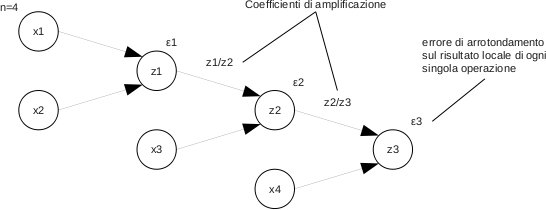
\includegraphics{fig/algoritmo1.jpg}
\caption{Algoritmo $1$.}
\end{figure}
\end{flushleft}
Per $n$ addendi l'errore complessivo finale sarà:
\[
\varepsilon^{n-1}= \varepsilon^{(n-1)} + \underbrace{\frac{z^{(n-2)}}{z^{(n-1)}}
\cdot\varepsilon^{n-2}}_{\textrm{errore trascinato dagli addendi}}.
\]
Dove $\varepsilon^{n-2}$ è l'errore complessivo che si è annidato sul 
penultimo nodo del grafo.

\[\varepsilon^{n-1}=\varepsilon^{(n-1)} + \frac{z^{(n-2)}}{z^{(n-1)}} \left(
\varepsilon^{(n-2)} +\frac{z^{(n-3)}}{z^{(n-2)}}\varepsilon^{n-3} \right)\]
\[= \varepsilon^{(n-1)} + \frac{z^{(n-2)}}{z^{(n-1)}}\varepsilon^{(n-2)} +
\frac{z^{(n-3)}}{z^{(n-1)}}\left(\varepsilon^{(n-3)} + \frac{z^{(n-4)}}{z^{(n-3)}}
\right)\]
\[\vdots\]
\[= \varepsilon^{(n-1)} + \frac{z^{(n-2)}}{z^{(n-1)}}\varepsilon^{(n-2)} +
\frac{z^{(n-3)}}{z^{(n-1)}}\varepsilon^{(n-3)} + \cdots + \frac{z^{(1)}}{z^{(n-1)}}
\varepsilon^{(1)} = \frac{1}{z^{(n-1)}}\sum_{i=1}^{n-1}z^{(1)}\varepsilon^{(i)}.
\]

Allora:
\[\varepsilon_{\textrm{alg}} = \frac{1}{f(\underline{x})} \cdot \sum_{i=1}^{n-1}
\left(\sum_{j=1}^{i+1}x_j\right) \cdot \varepsilon^{(i)}.\]

\begin{osse}
In generale \emph{non è possibile} dare \emph{limitazioni} per 
$\varepsilon_{\textrm{alg}}$ che non dipendono dai dati.
\end{osse}

Se $\left\{x_i\right\}$ sono tutti dello stesso segno, vale:
\[\left|\sum_{j=1}^{i+1}x_j\right| \leq \left|f(x)\right|, \quad i = 1, \ldots, 
n-1.\]

Allora:
\[|\varepsilon_{\textrm{alg}}| \leq \frac{1}{|f(\underline{x})|}
\sum_{i=1}^{n-1}\left|f(x)\right| \left|\varepsilon^{(i)}\right| \leq
(n-1)\cdot \verb eps  \qquad \textrm{crescita lineare.}\]

L'algoritmo è numericamente ben condizionato per $n$ piccoli, altrimenti
non lo è. In questo caso cosa possiamo fare?

\subsubsection{Algoritmo 1.2.}
Supponiamo di dare gli addendi in ordine di modulo non decrescente, la 
successione delle medie è ancora in modulo non decrescente:
\[\frac{1}{i}\left|\sum_{j=1}^ix_j\right| \leq \frac{1}{i+1}\left|
\sum_{j=1}^{i+1}
x_j\right| \leq \frac{1}{n}|f(\underline{x})|.\]

Allora:
\[|\varepsilon_{\textrm{alg}}| \leq \frac{1}{|f(\underline{x})|}\cdot 
\sum_{i=1}^{n-1}\left|\sum_{j=1}^{i+1}x_j\right| \cdot |\varepsilon^{(i)}| \leq 
\frac{1}{|f(\underline{x})|}\sum_{i=1}^{n-1}\frac{(i+1)f(\underline{x})}{n}
\cdot \verb eps =
\]
\[= \frac{eps}{n} \sum_{i=1}^{n-1}(i+1) < \frac{n+1}{2} \cdot\verb eps .\]

\[\longrightarrow \
|\varepsilon_{\textrm{alg}}| < \frac{n+1}{2} \cdot\verb eps \qquad 
\textrm{crescita lineare.}\]

\begin{osse}
La stima è migliorata di un coefficiente $\frac{1}{2}$.
\end{osse}

\subsection{Algoritmo 2.}
Addizioni in parallelo.

Sia $n = 2^p$, con $p$ intero positivo.
\begin{flushleft}\samepage
\textbf{Poniamo:}\\
$v_j^{(0)} = x_j, \quad j = 1, \ldots, n;$\\
$v_j^{(i)} = v_{2j -1}^{(i-1)} + v_{2j}^{i-1}, \quad j = 1, \ldots, \frac{n}{2^i};
\quad i = i, \ldots, p;$\\
$f(\underline{x}) = v_1^{(p)}.$
\begin{figure}[!ht]
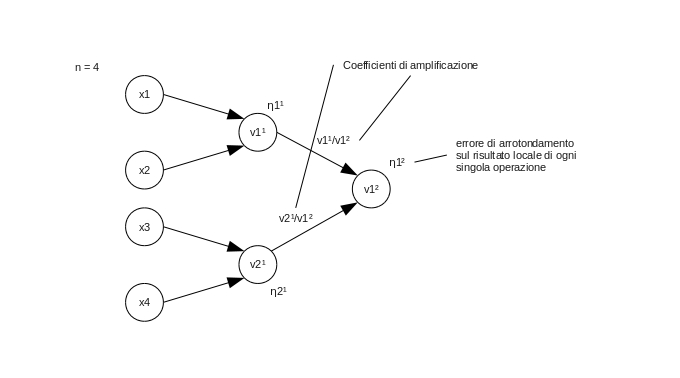
\includegraphics[scale=.75]{fig/algoritmo2.jpg}
\caption{Algoritmo $2$.}
\end{figure}
\end{flushleft}
\begin{prop}
L'errore algoritmico è quantificabile come:
\[\varepsilon_{\textrm{alg}} = \frac{1}{f(\underline{x})}\sum_{i=1}^p
\sum_{j=1}^{\frac{n}{2^i}}v_j^{(i)}\eta_j^{(i)}.\]

Poiché, dati gli $x_i$ dello stesso segno, si ha:
\[\sum_{j=1}^{\frac{n}{2^i}}\left|v_j^{(i)}\right| = |f(\underline{x})| 
\quad i = 0,
\ldots, p\]
risulta quindi:
\[|\varepsilon_{\textrm{alg}}| < \max_{i,j}\left|\eta_j^{(i)}\right|\cdot
\sum_{i=1}^p
\sum_{j=1}^{\frac{n}{2^i}}\frac{\left|v_j^{(i)}\right|}{|f(\underline{x})|}
= \max_{i,j}\left|v_j^{(i)}\right|\cdot p < \verb eps \cdot \log_2n.\]

\[|\varepsilon_{\textrm{alg}}| < \verb eps \cdot \log_2n.\]
\end{prop}
\begin{dimo}
Per $n = 2^k$ addendi l'errore algoritmico complessivo sarà:
\[\varepsilon_{\textrm{alg}} = \eta_1^{k} = \eta_1^{(k)} + \eta_1^{(k-1)} \cdot
\frac{v_1^{(k-1)}}{v_1^{(k)}} + \eta_2^{(k-1)}\cdot\frac{v_2^{(k-1)}}{v_1^{(k)}}.\]
\textbf{Ipotesi induttiva:}
\[\eta_1^{k} = \frac{1}{v_1^{(k)}} \cdot \sum_{i=1}^k\sum_{j=1}^{\frac{n}{2^i}^* }
v_j^{(i)}\eta_j^{(i)}, \quad
\eta_2^{k} = \frac{1}{v_2^{(k)}} \cdot \sum_{i=1}^k\sum_{j=1}^{2^{k+1-i}}
v_j^{(i)}\eta_j^{(i)}.\]
Nota $*: \ \frac{n}{2^i} = \frac{2^k}{2^i} = 2^{k-i}$.
\end{dimo}

\hyphenation{
Barrow
Binet
Cavalieri
Cotes
Chebyshev
Cholesky
Cramer
Gauss
Faber
Hausdorff
Householder
Lagrange
Laplace
Lebesque
Newton
Rolle
Runghe
Simpson
Sturm
tras-for-ma-zio-ne
Torricelli
}

\chapter{Integrazione Numerica.}
\textbf{Problema:}\\ \emph{calcolo numerico} dell'integrale definito di una
funzione $f \colon [a,b] \to \rr$, integrabile in $[a,b]$,  cioé $\int_a^b
f(x)dx$ mediante una formula del tipo:
\[\sum_{i=0}^n\omega_if(x_i) = \omega_0f(x_0)+ \omega_1f(x_1)+ \cdots 
+ \omega_nf(x_n),\]
dove $x_i \in [a,b], \ i = 0, \ldots, n$, sono detti \emph{nodi} e sono 
distinti, $\omega_i, \ i=0, \ldots, n$ sono detti \emph{pesi}.
\begin{flushleft}
\textbf{Analisi dell'errore:}
\[R_n(f) := \int_a^bf(x)dx - \sum_{i=0}^n\omega_if(x_i).\]
Possiamo calcolare $R_n(f)$ esattamente solo quando abbiamo $\int_a^bf(x)dx$,
quando non è possibile ricavare esattamente il valore dell'integrale è
possibile usare le formule di quadratura.
\end{flushleft}

\section{Formule (di quadratura) interpolatorie.}
Fissato $n \in \nn$ si scelgono $n+1$ nodi $\{x_i\}_{i=0}^n$ in $[a,b]$, con
$x_i \neq x_j$ per $i \neq j$; quindi si approssima $f(x)$ con il suo 
polinomio interpolatore $p_n(x)$ nei nodi fissati.
I punti base del polinomio sono: $x_0, \ldots, x_n$, in cui si calcolano i
valori della funzione: $f(x_0), \ldots, f(x_n)$.
\begin{osse}
$f(x)$ deve essere definita nei nodi di integrazione.
\end{osse}
Si ottiene allora:
\[\int_a^bf(x)dx = \int_a^bp_n(x)dx + \int_a^bE_n(x)dx.\]
\[\int_a^bf(x)dx = \sum_{i=0}^nf(x_i)\cdot \int_a^bL_i(x)dx + R_n(f).\]
$E_n(x)$ è l'errore di interpolazione, $L_i(x)$ sono i polinomi elementari di
Lagrange. Il \emph{resto} $R_n(f)$ è così definito:
\[R_n(f) = \int_a^bE_n(x)dx,\]
se $f \in \cc^{n+1}([a,b])$ si ha:
\[R_n(f) = \int_a^bw(x)\frac{f^{(n+1)}(\xi-x)}{(n+1)!}
dx.\]

Posto $\omega_i = \int_a^bL_i(x)dx, \ i = 0, \ldots, n$ si ottiene, 
trascurando il resto, la formula di quadratura:
\begin{equation}\label{eq14.1}
\int_a^bf(x)dx \simeq \sum_{i=0}^n\omega_if(x_i).
\end{equation} 

\begin{defi}La formula \ref{eq14.1}, in cui i pesi sono definiti da:
\[
\omega_i = \int_a^bL_i(x)dx, \quad i = 0, \ldots, n;
\]
viene detta formula di \emph{quadratura interpolatoria}.
\end{defi}

\begin{prop}
Una formula di quadratura interpolatoria integra esattamente almeno tutti
i polinomi di grado minore o uguale ad $n$.
\end{prop}
\begin{dimo}
Sia $p_n \in \PP_n$, allora:
\[R_n(f) = \int_a^bE_n(x)dx = \int_a^b\left(f(x)-p_n(x)\right)dx = 0.\]
Poiché $f(x) = p_n(x)$ per esistenza ed unicità del polinomio interpolante.
\end{dimo}

\begin{defi}
Una formula di quadratura si dice avere \emph{grado di precisione} $n$ se
integra esattamente tutti i polinomi di grado minore o uguale ad $n$ (resto
nullo) ed esiste $q \in \PP_{n+1}$ tale che $R_n(q) \neq 0$.
\end{defi}

\begin{osse}
Una formula di quadratura interpolatoria ha grado di precisione almeno $n$.
\end{osse}

\begin{teo}
Fissato $n \in \nn$, e fissati $n+1$ nodi distinti $\{x_i\}_{i=0}^n$ in $[a,b]$
esiste al più ($\exists!$) una formula di quadratura con grado di precisione
\emph{almeno} $n$, che quindi coincide con la formula di quadratura 
interpolatoria. 
\end{teo}

\begin{dimo}
Occorre imporre che $ \sum_{i=0}^n\omega_if(x_i)$ integri esattamente i 
polinomi di grado $\leq n$. Imponiamo quindi $n+1$ condizioni:
\[\left\{
\begin{array}{lr}
\sum_{i=0}^n\omega_i\cdot 1 = \int_a^b 1dx = b-a& x^{0} \\
\sum_{i=0}^n\omega_i\cdot x_i = \int_a^b xdx = \frac{b^2-a^2}{2}& x^{1} \\
\sum_{i=0}^n\omega_i\cdot x_i^2 = \int_a^b x^2dx = \frac{b^3-a^3}{3}& x^{2} \\
\vdots \\
\sum_{i=0}^n\omega_i\cdot x_i^n = \int_a^b x^ndx = 
\frac{b^{n+1}-a^{n+1}}{n+1}& x^{n}
\end{array}\right.
\]

\[\left\{
\begin{array}{l}
\omega_0 + \omega_1 + \cdots + \omega_n = b-a \\
\omega_0x + \omega_1x + \cdots + \omega_nx = \frac{b^2-a^2}{2} \\
\omega_0x^2 + \omega_1x^2 + \cdots + \omega_nx^2 = \frac{b^3-a^3}{3}\\
\vdots \\
\omega_0x^n + \omega_1x^n + \cdots + \omega_nx^n = 
\frac{b^{n+1}-a^{n+1}}{n+1}
\end{array}\right.
\]
La matrice del sistema risulta quindi:
\[\left[
\begin{array}{cccc}
1 & 1 & \cdots & 1 \\
x_0 & x_1 & \cdots & x_n \\
\vdots & \vdots & & \vdots\\
x_0^n & x_1^n & \cdots & x_n^n
\end{array}\right],
\]
ovvero la matrice trasposta di Vandermonde. Se i nodi sono distinti, il
determinante è diverso da $0$. L'unicità è garantita dal fatto che il
determinante non sia nullo, tuttavia a livello di calcolo (dei $\omega_i$) è
meglio percorrere un'altra strada.
\end{dimo}

\begin{prop}
Il massimo grado di precisione ottenibile con una formula di quadratura a
$n+1$ nodi distinti è $2n +1$.
\end{prop}
\begin{dimo}
Sia $Q(x) = \prod_{j=0}^n(x-x_j)^2 \in \PP_{2n+1}$. Allora:
\[R_n(Q) = \underbrace{\int_a^bQ(x)dx}_{ > 0} - 
\underbrace{\sum \omega_i Q(x_i)}_{=0} > 0.\]
\end{dimo}
$R_n(Q)$ sono le formule di quadratura gaussiana. Cosa possiamo cambiare?

La scelta dei nodi (non lo vedremo nel corso di Analisi Numerica $1$).

\section{Formule di quadratura di Newton-Cotes chiuse.}

Sono formule di quadratura \emph{interpolatorie} dove i nodi $x_i^{(n)}, \ i=0,
\ldots, n$
sono fissati ed equidistanti in $[a,b]$. Fissato $n \in \nn^+$ e posto
$h = \frac{b-a}{n}$, i nodi sono dati da:
\[x_i^{(n)} = a+ih, \quad i = 0, \ldots, n.\]
I pesi sono:
\[\omega_i = \int_a^bL_i(x)dx = \int_a^b\prod_{\substack{j = 0 \\ j \neq i}}^n 
\frac{x-x_j}{x_i-x_j}dx,\]
ponendo $x = a+sh$ si ha: 
\[
\int_a^b\prod_{\substack{j = 0 \\ j \neq i}}^n 
\frac{x-x_j}{x_i-x_j}dx =
\int_0^n\prod_{\substack{j = 0 \\ j \neq i}}^n 
\frac{\cancel{a} +sh \cancel{-a} -jh}{\cancel{a} +ih \cancel{-a} -jh}
ds.\]
\[
\omega_i = h \int_0^n\prod_{\substack{j = 0 \\ j \neq i}}^n \frac{s-j}{i-j}ds
= h \cdot \alpha_i^{(n)}.
\]

\begin{notabene}
Si dicono formule chiuse quando $a,b$ sono nodi, mentre si dicono aperte
quando $a,b \notin \{x_i\}$.
\end{notabene}

\begin{defi}
$\alpha_i^{(n)}$ è detta \emph{costante di Newton-Cotes}, indipendente da $a$ 
e $b$.
\[\int_a^bf(x)dx \approx h \sum_{i=0}^n \alpha_i^{(n)} f(x_i^{(n)}).\]
\end{defi}

\begin{osse}
Valgono le seguenti proprietà:
\begin{itemize}
\item[$\bullet$]$\alpha_i^{(n)} = \alpha_{n-i}^{(n)}$;
\item[$\bullet$]$\sum_{i=0}^n\alpha_i^{(n)} = n$.
\end{itemize}
\end{osse}
\begin{dimo}
\begin{itemize}
\item[$\bullet$]$\alpha_i^{(n)} = \alpha_{n-i}^{(n)}$;
\[\alpha_{n-i}^{(n)} = \int_0^n\prod_{\substack{j = 0 \\ j \neq n-i}}^n 
\frac{s-j}{n-i-j}ds
\]
ponendo $k = n-j$ si ha:
\[\alpha_{n-i}^{(n)} =\int_0^n\prod_{\substack{k = 0 \\ k \neq i}}^n \frac{s-n+k}{k-i}
ds
= \int_0^n\prod_{\substack{k = 0 \\ k \neq i}}^n \frac{n-s-k}{i-k}ds\]
ponendo $t= n-s$:
\[\alpha_{n-i}^{(n)} = \int_0^n\prod_{\substack{k = 0 \\ k \neq i}}^n \frac{t-k}{i-k}
dt
= \alpha_{i}^{(n)}.\]
\item[$\bullet$]$\sum_{i=0}^n\alpha_i^{(n)} = n$.
\[\int_a^b1\cdot dx = h \sum_{i=0}^n \alpha_i^{(n)}\ \leadsto\ \sum_{i=0}^n 
\alpha_i^{(n)} =
\frac{b-a}{h} = n. \]
\end{itemize}
\end{dimo}

\subsection{Formula dei trapezi ($n=1$).}
\[x_0^{(1)} = a, \quad x_1^{(1)} = a+h = a+ \frac{b-a}{1} = b.\]
\[\alpha_0^{(1)}= \int_0^1 \frac{s-1}{0-1}ds = \left[-\frac{s^2}{2} +s
\right]_0^1
= \frac{1}{2}.\]
Inoltre per simmetria si ha $\alpha_0^{(1)}=\alpha_1^{(1)} = \frac{1}{2}$.
\[\int_a^bf(x)dx = \frac{b-a}{2}[f(a)+f(b)] + R_1(f).\]


\subsection{Formula di Cavalieri-Simpson ($n=2$).}
\[x_0^{(2)} = a, \quad x_1^{(2)} = a+h = a+ \frac{b-a}{2} = \frac{a+b}{2},
\quad x_2^{(2)} = b.\]

\[\alpha_0^{(n)}=
\int_0^2 \frac{s-1}{0-1} \cdot \frac{s-2}{0-2}ds =
\frac{1}{2} \int_0^2(1-s)(2-s)ds = 
\]
\[= 
\frac{1}{2} \int_0^2(s^2-2s-s+2)ds = \frac{1}{2}\left[
\frac{1}{3}s^3 - s^2 -\frac{1}{2}s^2 +2s\right]_0^2 =
\]
\[=\frac{1}{2}\left(
\frac{2^3}{3} - 3 \frac{2^2}{2} + 2\cdot 2\right) = \frac{4}{3} -3 +2 =
\frac{1}{3}.
\]

\[\alpha_1^{(2)} =
\int_0^2 \frac{s-0}{1-0} \cdot \frac{s-2}{1-2}ds =
\int_0^2 s(2-s)ds = \int_0^2-(s^2+2s) ds =
\]
\[=
\left[\frac{2s^2}{2} - \frac{s^3}{3}\right]_0^2 = 
\frac{2 \cdot2^2}{2} - \frac{2^3}{3} = \frac{4}{3}.
\]

\[\alpha_2^{(n)} = \alpha_0^{(n)}= \frac{1}{3}.\]

\[\alpha_0^{(n)} +\alpha_1^{(n)} + \alpha_2^{(n)} = \frac{1}{3} + \frac{4}{3} + 
\frac{1}{3} = 2
= n \qquad \rightarrow \textrm{ok.}\]

\[
\omega_0 = h \cdot \alpha_0^{(n)} = \frac{b-a}{2}\cdot \frac{1}{3} = \frac{b-a}{6}.
\]
\[
\omega_1 = h\cdot \alpha_1^{(n)} = \frac{b-a}{2}\cdot\frac{4}{3} =\frac{2(b-a)}{3}.
\]
\[
\omega_2 = h \cdot \alpha_2^{(n)} = \frac{b-a}{2}\cdot \frac{1}{3} = \frac{b-a}{6}.
\]

\[
\int_a^bf(x)dx = \frac{b-a}{2} \sum_{i=0}^2\alpha_i^{(2)} f(x_i) = \frac{b-a}{2}
\left[\alpha_0^{(n)} f(x_0)+ \alpha_1^{(n)} f(x_1)+\alpha_2^{(n)} f(x_2)\right]=\]
\[=
\frac{b-a}{2}\left[
\frac{1}{3} f(a)+ \frac{4}{3}f\left(\frac{a+b}{2}\right) + \frac{1}{3}
f(b)\right]=\]
\[=\frac{b-a}{6}f(a) + \frac{2(b-a)}{3}f\left(\frac{a+b}{2}\right)+
\frac{b-a}{6}f(b).
\]

\[
\int_a^bf(x)dx = \frac{h}{3}\left[f(a)+4f\left(\frac{a+b}{2}\right)
+ f(b)\right].
\]


\subsection{Formula dei tre ottavi ($n=3$).}
\[x_0^{(3)} = a, \quad x_1^{(3)} = a+h = a+ \frac{b-a}{3},
\quad x_2^{(3)} = a+\frac{2(b-a)}{3},\quad x_3^{(3)} = b.\]

\[\alpha_0^{(n)}=
\int_0^3 \frac{s-1}{0-1} \cdot \frac{s-2}{0-2}\cdot \frac{s-3}{0-3}ds =
\int_0^3(1-s)\frac{(2-s)}{2}\frac{(3-s)}{3}ds.
\]
\[\alpha_0^{(n)}=
\frac{1}{6}\int_0^3(1-s)(2-s)(3-s)ds = \frac{1}{6}\int_0^3 \left(
-s^3 +6s^2 -11s +6\right)ds.
\]
\[\alpha_0^{(n)}=
\frac{1}{6}\left[-\frac{s^4}{4} +2s^3 -\frac{11 s^2}{2} +6s\right]_0^3
= \frac{1}{6}\left[-\frac{81}{4}+ 54 -\frac{99}{2} +18 \right].
\]
\[\alpha_0^{(n)}=
\frac{1}{6}\left[\frac{-81-198}{4} +\frac{216}{4} + \frac{72}{4}\right]
= \frac{1}{6} \cdot \frac{9}{4} = \frac{1}{2}\cdot \frac{3}{4} = \frac{3}{8}.
\]

Possiamo, questa volta, calcolare $\alpha_1^{(3)}$ senza utilizzare le formule 
integrali, poiché:
\[
\alpha_0^{(3)} + \alpha_1^{(3)} + \alpha_2^{(3)} + \alpha_3^{(3)} = 3.
\]
Dai calcoli precedenti e dal fatto che $\alpha_1^{(3)} = \alpha_2^{(3)}$ 
otteniamo:
\[
\frac{3}{8} + \alpha_1^{(3)} + \alpha_1^{(3)} + \frac{3}{8} = 3\ 
\Longrightarrow\
2\cdot \alpha_1^{(3)} = 3 - \frac{\cancelto{3}{6}}{\cancelto{4}{8}}.
\]
\[
\alpha_1^{(3)} = \frac{3}{2}-\frac{3}{8} = \frac{12-3}{8} = \frac{9}{8} = 
\alpha_2^{(3)}.
\]

\[
\int_a^bf(x)dx = h\left[\frac{3}{8}f(a) + \frac{9}{8}f\left(a +\frac{b-a}{3}
\right) + \frac{9}{8} f\left(a+\frac{2(b-a)}{3}\right) + \frac{3}{8}f(b)
\right].
\]
\[
\int_a^bf(x)dx = \frac{3}{8} h \left[
f(a) + 3 f\left(a +\frac{b-a}{3}\right) + 3f\left(a+\frac{2(b-a)}{3}\right)
+f(b)\right] + R_3(f).
\]

\begin{ese}
Dato un integrale:
\[\int_0^1x^3dx,\]
approssimarlo con la formula dei trapezi e di Cavalieri-Simpson, determinare
per questo problema test (solo soluzione chiusa) l'errore assoluto per le due
formule.

\begin{svol}
Calcoliamo per primo il valore dell'integrale definito:
\[\int_0^1x^3dx = \left[\frac{x^4}{4}\right]_0^1 = \frac{1}{4}.\]
\begin{itemize}
\item[$\bullet$]Formula dei trapezi:
\[\int_0^1x^3dx = h(f(a)+f(b)) = \frac{1}{2}(1+0) = \frac{1}{2} + R_1(f).\]
\item[$\bullet$]Formula di Cavalieri-Simpson:
\[\int_0^1x^3dx = \frac{h}{3}\left(f(a)+4f\left(\frac{a+b}{2}\right) +f(b)
\right) = \frac{1}{6}\left(0 + \frac{1}{2} + 1\right) =\]
\[= \frac{1}{12} + 
\frac{1}{6} = \frac{3}{12} = \frac{1}{4} + R_2(f).\]
\end{itemize}
Si ha quindi che:
\[R_1(f) = - \frac{1}{4}, \quad R_2(f) = 0.\]

La formula dei trapezi ha grado di precisione almeno $1$, è quindi giusto che
commetta un errore, la formula di Cavalieri-Simpson invece ha grado di
precisione almeno $2$. Questa funzione però è di grado $3$ e viene integrata
perfettamente. E' questo un caso?
\end{svol}

No. E' una proprietà delle formule di Newton-Cotes con $n$ pari (numero
dispari di nodi) che hanno precisione almeno $n+1$.
\end{ese}

\begin{osse}
Le formule di Newton-Cotes hanno grado di precisione almeno $n$ essendo
formule interpolatorie.
\end{osse}

\begin{prop}
La  formula dei trapezi ha grado $1$ e precisione \emph{esattamente} $1$.
\end{prop}
\begin{dimo}
Sia $q(x) = (x-a)(x-b) \in \PP_2$, allora:
\[\begin{array}{lcl}
R_1(q) & = & \displaystyle
             \int_a^bq(x)dx - h\sum_{i=0}^1\alpha_i^{(1)}q(x_i^{(1)}) \\
      & = & \underbrace{\int_a^bq(x)dx}_{< 0} -\frac{b-a}{2}
\underbrace{[q(a)+q(b)]}_{\equiv 0} \neq 0.
\end{array}\]
\end{dimo}

\begin{prop}
Se $n$ è pari (numero di nodi dispari), le formule di quadratura di
Newton-Cotes a $n+1$ nodi hanno almeno grado di precisione $n+1$.
\end{prop}
\begin{dimo}
Le formule di quadratura considerate, essendo interpolatorie, integrano
esattamente tutti i polinomi di grado minore o uguale ad $n$.

Sia ora $q \in \PP_{n+1}$, possiamo allora scrivere $q$ nella seguente forma:
\[q(x) =\overline{a} (x-x_{\frac{n}{2}})^{n+1} + q_n(x), \quad x_{\frac{n}{2}}=
\frac{a+b}{2}, \ q_n \in \PP_n.\]

\[\longrightarrow \
\int_a^bq(x)dx = \overline{a}\int_a^b(x-x_{\frac{n}{2}})^{n+1}dx + \int_a^bq_n(x)dx
.\]

Poiché il polinomio $(x-x_{\frac{n}{2}})^{n+1}$ è di grado dispari e la funzione
è antisimmetrica rispetto al punto medio dell'intervallo di integrazione si 
ha:
\[\int_a^b(x-x_{\frac{n}{2}})^{n+1}dx = 0.\]

\[\longrightarrow \
\int_a^bq(x)dx = \int_a^bq_n(x)dx = h\sum_{i=0}^n\alpha_i^{(n)}q_n(x_i).\]
Poiché $x_i - x_{\frac{n}{2}} = -(x_{n-1} - x_{\frac{n}{2}})$ per $i=0,\ldots,n$ e
$\alpha_{n-i}^{(n)} = \alpha_i^{(n)}$ si ha:
\[
= \sum_{i=0}^n\alpha_i^{(n)}(x_i - x_{\frac{n}{2}})^{n+1} \equiv 0.
\]

\[\longrightarrow \
\int_a^bq(x)dx = h \left(\overline{a}\sum_{i=0}^n\alpha_i^{(n)}(x_i - 
x_{\frac{n}{2}})^{n+1} + \sum_{i=0}^n\alpha_i^{(n)}q_n(x_i)\right)
\]
\[
= h \cdot \sum_{i=0}^n\alpha_i^{(n)}q_n(x_i)
\]
\end{dimo}

\begin{prop}
La formula di Cavalieri-Simpson ha grado di precisione \emph{esattamente} $3$.
\end{prop}
\begin{dimo}
Sia $q(x) = (x-a)(x-\frac{a+b}{2})^2(x-b) \in \overline{\PP}_n$, allora:
\[
R_2(q) = \int_a^bq(x)dx - h \sum_{i=0}^2\alpha_i^{(2)}q(x_i^{(2)}).
\]
\[
R_2(q) = \underbrace{\int_a^bq(x)dx}_{< 0} - \frac{h}{3} \underbrace{
\left[q(a)+ 4q(\frac{a+b}{2})+ q(b)\right]}_{\equiv 0} \neq 0.
\]
\end{dimo}

\subsection{Errore di integrazione numerica.}
Per le varie formule di quadratura viste fino ad ora abbiamo visto che
approssimano un risultato che si discosta dal valore reale per un resto che 
abbiamo denotato con $R_i$. Cerchiamo ora di stimare questo errore.
\begin{teo}
Sia $n \in \nn$ dispari e $f \in \cc^{n+1}([a,b])$, allora esiste $\xi \in 
(a,b)$ tale che:
\[ R_n(f) = K_n \frac{f^{(n+1)}(\xi)}{(n+1)!}
\cdot h^{n+2}, \quad h = \frac{b-a}{n}.\]
\[K_n = \int_0^n \mathcal{T}_n(t)dt, \quad 
\textrm{con } \mathcal{T}_n = \prod_{i=0}^n(t-i).\] 
\end{teo}

\begin{notabene}
$\xi$ non è dato saperlo, ovvero non possiamo calcolare esattamente l'errore,
però lo possiamo stimare.
\end{notabene}

In particolare per la formula dei trapezi si ha:
\[R_1(f) = - \frac{1}{12}f''(\xi)h^3.\]

\begin{dimo}Caso $n = 1$:
\[
R_1(f) = \int_a^b\left[f(x)-p(x)\right]dx = \int_a^b\underbrace{(x-a)(x-b) 
\frac{f''(\xi)}{2!}}_{\textrm{(*) errore di interpolazione}}dx.
\]
Si applica dunque il Teorema della media generalizzato al prodotto di due 
funzioni: una continua $g$ (= (*)) e un'altra che non cambia segno $r = 1$ 
nell'intervallo di interpolazione:
\[
R_1(f) =\frac{f''(\xi)}{2!}\int_a^b(x-a)(x-b)dx .
\]
Ponendo $x = a +th$, $h = b-a$ si ha:
\[
R_1(f) =\frac{f''(\xi)}{2!}\int_0^1th(t-1)hhdt = h^3\frac{f''(\xi)}{2!}\int_0^1
\underbrace{(t-0)(t-1)}_{\mathcal{T}(t)}dt.
\]
\[
R_1(f) = h^3\frac{f''(\xi)}{2!}\left[\frac{t^3}{3} -\frac{t^2}{2}\right]_0^1
= - \frac{1}{12}f''(\xi)h^3.
\]
\end{dimo}

Se $b-a = 1000$ avremmo $R_1 \sim 1000^3$, ovvero un errore enorme!
Dobbiamo quindi integrare su intervalli tali che $h<1$.

\begin{teo}
Sia $n \in \nn$ pari e $f \in \cc^{n+2}([a,b])$, allora esiste $\xi \in 
(a,b)$ tale che:
\[
R_n(f) = \overline{K}_n \frac{f^{(n+2)}(\xi)}{(n+2)!} h^{n+3}, 
h = \frac{b-a}{n}.
\]
\[
\overline{K}_n = \int_0^nt\mathcal{T}(t)dt, \quad
\textrm{con } \mathcal{T}(t)= \prod_{i=0}^n(t-i).
\]
\end{teo}
In particolare per la formula di Cavalieri-Simpson si ha:
\[
R_2(f) = -\frac{1}{90}f^{(iv)}(\xi)h^5.
\]

\begin{dimo}Caso $n=2$ (formule di quadratura di Cavalieri-Simpson):
\[
R_2(f) = \int_a^bf(x)dx - h \sum_{i=0}^2\alpha_i^{(2)}f(x_i^{(2)}).
\]
Sia $\overline{p} \in \PP_3$ il polinomio interpolante $f(x)$ nei nodi:
\[x_0^{(2)}=a, \ x_1^{(2)}= \frac{a+b}{2}, \  x_2^{(2)}=b,\]
e sia $f'(x)$, calcolata nel nodo $x_1^{(2)}$, uguale a $c = a + h = 
\frac{a+b}{2}$. Ricordiamo inoltre che la formula di quadratura di 
Cavalieri-Simpson ha grado di precisione $3$.

\[
R_2(f) = \int_a^b\left[f(x) - \overline{p}(x)\right]dx =
\int_a^b(x-a)(x-c)^2(x-b) \frac{f^{(iv)}(\xi_x)}{4!}dx.
\]
Sfruttando il teorema della media generalizzata si ha:
\[R_2(f) =
\frac{f^{(iv)}(\xi_x)}{4!}  \int_a^b(x-a)(x-c)^2(x-b)dx.
\]
Ponendo $x = a + th$ e ricordando che $h = \frac{b-a}{2}$ si ha:
\[\begin{array}{lcl}\displaystyle
R_2(f) & = &\displaystyle \frac{f^{(iv)}(\xi_x)}{4!} \int_0^2t(t-1)^2(t-2)h^5dt \\
& = &\displaystyle h^5 \frac{f^{(iv)}(\xi_x)}{4!}
\underbrace{\int_0^2t\mathcal{T}(t)dt}_{\neq 0} - \cancelto{0}{
h^5 \frac{f^{(iv)}(\xi_x)}{4!}\underbrace{\int_0^2\mathcal{T}(t)dt}_{=0}}\\
& = &\displaystyle h^5\frac{f^{(iv)}(\xi_x)}{4!}\left[\frac{1}{5}t^5-
\frac{3}{4}t^4+\frac{2}{3}t^3\right]_0^2 \\
& = &\displaystyle -\frac{1}{90}\cdot f^{(iv)}(\xi_x)\cdot h^5.
\end{array}\]
\end{dimo}

\begin{ese}
Approssimare l'integrale:
\[
\int_0^1 e^{-x^2}dx
\]
commettendo un errore non superiore a $0.5 \cdot 10^-2$.
\end{ese}
\begin{svol}
\begin{itemize}
\item Utilizziamo le formule chiuse di Newton Cotes.
\item Poniamo $n = 1$ con $E_1 = -\frac{1}{12}h^3f''(\xi)$.

In questo caso $f''(x) = 2(2x^2 -1)e^{-x^2}$ e $h = 1$, si ha 
dunque: \[\max_{x \in (0,1)}|f''(x)|=2, \]
facendo i calcoli otteniamo:\[E_1 \leq \frac{1}{6}.\]
\end{itemize}
Il risultato non è soddisfacente.
\begin{itemize}
\item Poniamo $n = 2$ con $E_2 = -\frac{1}{90}h^5f^{(iv)}(\xi)$.

In questo caso $f^{(iv)}(x) = 4(4x^4 -12x^2+3)e^{-x^2}$ e $h = \frac{1}{2}$, si ha 
dunque: \[\max_{x \in (0,1)}|f^{(iv)}(x)|=12, \]
facendo i calcoli otteniamo:\[E_2 \leq \frac{1}{240}.\]
\end{itemize}
Il risultato è soddisfacente.
\begin{itemize}
\item Calcoliamo ora l'integrale con la formula dei trapezi:

\[\int_0^1 e^{-x^2}dx = \frac{1}{6}\left[1 + 4e^{-\frac{1}{4}}+ e^{-1}\right]
= 0.7472\]
Commettendo un errore che al più sarà $0,0041 \leq 0.5\cdot 10^{-2}$.
\end{itemize}
\end{svol}

\section{Formule di quadratura di Newton-Cotes aperte.}
Le formule aperte di Newton-Cotes sono sempre formule interpolatorie, in cui
i nodi sono equispaziati, ma non interpolano gli estremi dell'intervallo.

Fissato $n \in \nn$ e posto $h = \frac{b-a}{n+2}$ i nodi sono dati da:
\[x_i = a + (i+1)h, \quad i = 0,\ldots,n.\]
\begin{osse} Vediamo i nodi più esterni: 

\begin{itemize}
\item[]$i = 0\ \longrightarrow\ x_0 = a + h \neq a$;
\item[]$i = n\ \longrightarrow\ x_n = a+ (n+1)h < b$.
\end{itemize}
\end{osse}

Data una generica formula interpolatoria analizziamo i pesi $\omega_i$ 
analogamente a quanto fatto per le formule chiuse.

\[\omega_i = \int_a^bL_i(x)dx = \int_a^b\prod_{\substack{j = 0 \\ j \neq i}}^n 
\frac{x-x_j}{x_i-x_j}dx,\]
ponendo $x = a+sh$ si ha: 
\[
\int_{-1}^{n+1}\prod_{\substack{j = 0 \\ j \neq i}}^n 
\frac{\cancel{a} +sh \cancel{-a} -jh}{\cancel{a} +ih \cancel{-a} -jh}
ds.\]
\[
\omega_i = h \int_{-1}^{n+1}\prod_{\substack{j = 0 \\ j \neq i}}^n \frac{s-j}{i-j}ds
= h \cdot \alpha_i^{(n)}.
\]

La struttura dei pesi è simile a quella delle formule chiuse, cambiano gli
estremi di integrazione ma godono delle stesse proprietà. In particolare
i pesi non dipendono dagli estremi.

Queste formule sono utili nel caso in cui si devono studiare funzioni non
integrabili agli estremi.
\begin{exe}Il seguente integrale non è calcolabile mediante formule chiuse:
\[\int_0^1\log(x)dx.\]
\end{exe}

\subsection{Formula del punto medio ($n=0$).}
\[
h = \frac{b-a}{2}, \quad x_0 = a+h = \frac{a+b}{2}, \quad \omega_0 = b-a
= h\cdot 2\ \Rightarrow\ \alpha_0^{(0)} = 2.
\]

\[
\int_a^bf(x)dx = (b-a)\cdot f\left(\frac{a+b}{2}\right) + R_0(f).
\]

\begin{figure}[ht!]\begin{center}
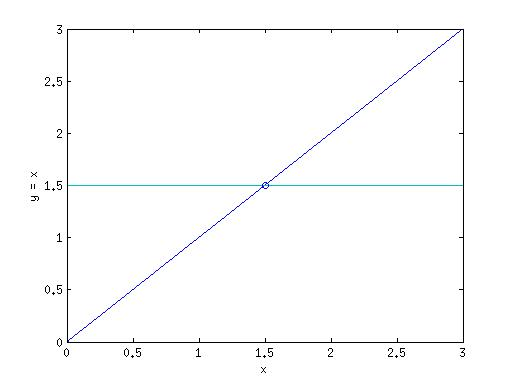
\includegraphics[scale=0.50]{fig/punto_medio.jpg}\end{center}
\caption{Integrale della funzione $f(x) = x$ nell'intervallo $(0,3)$ mediante
la formula del punto medio.}
\label{fig_puntomedio}\end{figure}

La formula del punto medio integra \emph{perfettamente} i polinomi di primo
grado (e inferiori), questo si può osservare chiaramente nell figura 
\ref{fig_puntomedio}.


\subsection{Errore di integrazione numerica.}
Analogamente a quanto fatto per le formule di Newton-Cotes chiuse, analizziamo
il resto dell'integrazione per stimarne l'errore.

\begin{teo}
Sia $n \in \nn$ dispari e $f \in \cc^{n+1}([a,b])$, allora esiste $\xi \in
(a,b)$ tale che:
\[
R_n(f) = K_n \cdot \frac{f^{n+1}(\xi)}{(n+1)!} \cdot h^{n+2}, \quad 
h = \frac{b-a}{n+2};
\]
\[
K_n = \int_{-1}^{n+1}\mathcal{T}_ndt, \quad \mathcal{T}_n = \prod_{i=0}^n(t-i).
\]
\end{teo}
\begin{teo}
Sia $n \in \nn$ pari e $f \in \cc^{n+2}([a,b])$, allora esiste $\xi \in
(a,b)$ tale che:
\[
R_n(f) = K_n \cdot \frac{f^{n+2}(\xi)}{(n+2)!} \cdot h^{n+3}, \quad 
h = \frac{b-a}{n+2};
\]
\[
K_n = \int_{-1}^{n+1}\mathcal{T}_ndt, \quad \mathcal{T}_n = \prod_{i=0}^n(t-i).
\]
\end{teo}
\begin{cor}
Le formule di Newton-Cotes aperte con $n$ dispari hanno grado di precisione
$n$, quelle con $n$ pari hanno grado di precisione $n+1$.
\end{cor}

\begin{osse}
In particolare la formula del punto medio integra \emph{esattamente} tutti i
polinomi di grado $\leq 1$.
\end{osse}

\begin{prop}
Sia $f \in \cc^{2}([a,b])$, ovvero $n = 0$, allora l'errore risulta:
\[
R_0(f) = \frac{1}{3}f''(\xi)h^3, \quad h = \frac{b-a}{2}.
\]
\end{prop}
\begin{dimo}
Poniamo $f$ nella generica ``forma di secondo grado'' $f(x) = (x-c)^2$, il
punto medio $x_0=\frac{a+b}{2}$ e $p$ il polinomio al più di primo
grado che interpola $f$ nel punto $x_0$. Sia ora la derivata prima
calcolata in $x_0$ uguale a $c$, ovvero $f'\left(x_0\right) = c$.

\[\begin{array}{lclr}
R_0(f) &=& \displaystyle \int_a^bf(x)dx - h\cdot \alpha_0 
\cdot f\left(x_0\right) & \textrm{per def.} \\
&=& \displaystyle\int_a^bf(x)dx - \underbrace{h\cdot \alpha_0\cdot
 p\left(x_0\right)}_{* = \int_a^bp(x)dx}& \textrm{def. di interpolazione}\\
&=& \displaystyle\int_a^b\left[f(x)-p(x)\right]dx & *\\
&=& \displaystyle\int_a^b\frac{(x-c)^2f''(\xi)}{2!}dx 
& \textrm{def. di errore di interp.}\\
&=& \displaystyle\frac{f''(\xi)}{2}\int_a^b(x-c)^2dx. & \textrm{teo. media gen.}
\end{array}\]
Poniamo ora $x = a + (t+1)\cdot h$, abbiamo che:
\[\begin{array}{lcl}
R_0(f) &=& \displaystyle\frac{f''(\xi)}{2}\int_{-1}^1t^2h^2hdt \\
&=& \displaystyle\frac{f''(\xi)}{2}\int_{-1}^1t^2h^3dt\\
&=& \displaystyle\frac{f''(\xi)}{2}\cdot h^3 \int_{-1}^1t^2dt \\
&=& \displaystyle\frac{f''(\xi)}{2}\cdot h^3 \left[\frac{t^3}{3}\right]_{-1}^1\\
&=& \displaystyle\frac{1}{3}\cdot h^3 \cdot f''(\xi).
\end{array}
\]
\end{dimo}

\part{Matlab.}
\label{Matlab.}
\hyphenation{
Matlab
}

\begin{comment}

\begin{codice}
\begin{verbatim}

\end{verbatim}
\end{codice}

\end{comment}

\chapter{Introduzione a Matlab.}
MATLAB (abbreviazione di Matrix Laboratory) è un ambiente per il calcolo 
numerico e l'analisi statistica che comprende anche l'omonimo linguaggio di 
programmazione creato dalla The MathWorks. MATLAB consente di manipolare 
matrici, visualizzare funzioni e dati, implementare algoritmi, creare 
interfacce utente, e interfacciarsi con altri programmi.

\begin{notabene}Il corso e \emph{sopratutto l'esame} di Laboratorio di 
Calcolo Numerico vertirà su esercizi da svolgersi in ambiente Matlab, per
esercitarsi è possibile usufruire dei computer in laboratorio. Per coloro che
volessero (o debbano) esercitarsi a casa, poiché Matlab è un software
proprietario, l'unico modo (legale) per ottenere il programma è l'acquisto.
Tuttavia esiste un'alternativa ``free'', Octave, che permette di fare gran parte
delle operazioni di Matlab con gli stessi comandi. D'ora in poi, nel seguente
testo, per specificare differenze o particolarità riguardanti Octave 
utilizzeremo un ``ambiente'' apposito come il seguente.
\end{notabene}

\begin{octave}
GNU Octave è un'applicazione software per l'analisi numerica parzialmente
 compatibile con MATLAB. Octave è rilasciato sotto licenza GPL, e quindi può 
essere liberamente copiato e usato. Il programma gira sotto sistemi Unix e 
Linux, oltre che su Windows e MAC OS X.

Ha un insieme di funzionalità fornite per il calcolo matriciale come rango e 
determinante o specialistiche come decomposizione ai valori singolari (SVD), 
fattorizzazione LU; sebbene le consenta la soluzione numerica di sistemi 
lineari non svolge calcolo simbolico o altre attività tipiche di un sistema 
di algebra computazionale.
\end{octave}

\section{Introduzione.}
Questo testo è di fatto una raccolta di appunti del corso di Laboratorio di
Calcolo Numerico del dipartimento di Matematica dell'Università di Parma, 
non ha lo scopo di sostituirne le lezioni o i libri di testo
consigliati. Pertanto sconsiglio di utilizzarlo come unica fonte di studio
o di esercitazione pratica.

Inoltre non verranno definite tutte le funzioni o risolti tutti gli esercizi
proposti durante il corso ed alcune altre cose saranno date per scontate
come ad esempio la descrizione o definizione di:
\begin{enumerate}
\item[-]Command Window,
\item[-]Command History,
\item[-]Workspace,
\item[-]alcune funzionio comandi ben descritti sul libro di testo.
\end{enumerate}

\section{Help.}
Il primo comando utile di Matlab è \verb1help1, serve, dato
un comando o una funzione, per ottenerne le istruzioni d'uso:
\begin{codice}
\begin{verbatim}
>> help nomecomando
>> help nomefunzione
\end{verbatim}
\end{codice}

\section{Variabili ed ambiente di lavoro.}
In Matlab tutte le variabili sono array, nello specifico una variabile singola
è un array di dimensione $1$. Nell'ambiente di lavoro (workspace) le variabili
vengono memorizzate e vi risiedono fino alla fine della sessione di lavoro o
fino a quando non viene utilizzato il comando \verb1clear1 che consente di
cancellarle, non vengono cancellati lo schermo e la history dei comandi.
Per cancellare il contenuto dello schermo si utilizza il comando \verb1clc1.
\begin{codice}
\begin{verbatim}
>> clear
\end{verbatim}
\end{codice}

Per definire (dichiarazione e inizializzazione) una variabile è sufficiente
scrivere la seguente istruzione:
\begin{codice}
\begin{verbatim}
>> x = 1

x =

     1
\end{verbatim}
\end{codice}
In questo modo verrà salvata nel Workspace la variabile di nome $x$, valore 
$1$, size $1\times 1$ e valore minimo e massimo dell'array. Di default gli 
attributi visibili delle variabili del Workspace dovrebbero essere questi, è
comunque possibile cambiarli dal menù a tendina ``view/Choose Columns''.

E' possibile evitare di visualizzare a schermo l'assegnamento della variabile
semplicemente utilizzando il carattere ``;'' a fine istruzione. Questo è
molto utile per array o matrici di grandi dimensioni.

\begin{codice}
\begin{verbatim}
>> v = [ 1 2 3 4 5 6 7 8 9 ]

v =

     1     2     3     4     5     6     7     8     9

\end{verbatim}
\end{codice}

\begin{codice}
\begin{verbatim}
>> v = [ 1 2 3 4 5 6 7 8 9 ];
>> 
\end{verbatim}
\end{codice}

Esiste una variabile speciale in Matlab chiamata \verb1ans1, questa è generata
automaticamente se non viene esplicitamente dato un nome ad una variabile,
tipicamente quando non viene assegnato il risultato di un operazione.
Proviamo a moltiplicare il nostro vettore $v$ per la variabile $x$ senza
assegnamento:
\begin{codice}
\begin{verbatim}
>> x*v

ans =

     1     2     3     4     5     6     7     8     9
\end{verbatim}
\end{codice}
Utilizzare la variabile \verb1ans1 non è un errore, occorre però fare 
attenzione poiché questa può essere sovrascritta durante il lavoro.

Nell'ambiente di lavoro è inoltre possibile cambiare il formato di 
rappresentazione dei numeri, di default l'ambiente dovrebbe essere inpostato
sul formato \verb1short1 ma è possibile cambiarlo con il comando \verb1format1.
\begin{codice}
\begin{verbatim}
>> x = 1/2

x =

    0.5000

>> format long
>> x = 1/2

x =

   0.500000000000000

>> 
\end{verbatim}
\end{codice}
Inizialmente $x$ ha quattro cifre dopo la virgola, impostando il formato 
\verb1long1 diventano quindici.
\begin{octave}In Octave le cifre del formato short sono cinque dopo la virgola,
si noti inoltre la differenza di stampa nella Command Window (che in Octave si
chiama Octave Terminal).
\begin{codice}
\begin{verbatim}
>>> x = 1/2
x =  0.50000
>>> format long
>>> x = 1/2
x =  0.500000000000000
\end{verbatim}
\end{codice}
\end{octave}

Matlab lavora con un sistema floating point in doppia precisione (si possono
aumentare i numeri dopo la virgola).

\subsection{Variabili speciali.}
In Matlab esistono alcune variabili speciali:
\begin{center}
\begin{tabular}{ll}
\verb1i1, \verb1j1 & unità immaginarie ($i^2 = -1, \ j^2 = -1$), \\
\verb1pi1 & pi greco, \\
\verb1realmax1 & il più grande numero di macchina, \\
\verb1realmin1 & il più piccolo numero di macchina, \\
\verb1Inf1 & $\infty$, ovvero un numero maggiore di \verb1realmax1, \\
\verb1nan1 & Not a number ($0/0$, etc.), \\
\verb1eps1 & epsilon macchina.
\end{tabular}\end{center}

\begin{codice}
\begin{verbatim}
>> pi

ans =

    3.1416
\end{verbatim}
\end{codice}

\subsection{Funzioni Built-In.}
In Matlab è possibile utilizzare una lista di funzioni ``pre-costruite'' come
\verb1sin1, \verb1cos1, etc... con la sintassi seguente:
\begin{center}
\begin{tabular}{ll}
\verb1sin(x)1 & calcola il seno della variabile \verb1x1, \\
\verb1cos(x)1 & calcola il coseno delella variabile \verb1x1, \\
\verb1sqrt(x)1 & calcola la radice quadrata di \verb1x1, \\
\verb1abs(x)1 & calcola il valore assoluto di \verb1x1, \\
\verb1log(x)1 & calcola il logaritmo naturale di \verb1x1, \\
\verb log10(x) & calcola il logaritmo di\verb1x1in base $10$.
\end{tabular}\end{center}

\begin{codice}
\begin{verbatim}
>> log(2)

ans =

    0.6931

>> log10(2)

ans =

    0.3010
\end{verbatim}
\end{codice}

Molte altre funzioni sono disponibili, per poterle visualizzare tutte è
possibile utilizzare il browser apposito cliccando sulla barra di navigazione
su Help/Function Browser, oppure premendo MAIUSC+F1.

\begin{octave}
La maggior parte delle funzioni sono presenti su Octave con lo stesso nome.
\begin{codice}
\begin{verbatim}
>>> log(2)
ans =  0.69315
\end{verbatim}
\end{codice}
Però, come già sottolineato, il formato short differisce per una cifra 
decimale, è quindi consigliabile usare il formato long.
Inoltre in Octave per visualizzare la lista è necessario andare sull'Help,
sempre sulla barra di navigazione: Help/Octave Help (anche premendo F1) e 
quindi in fondo all'indice delle pagine di aiuto, dopo le appendici,
cliccare su \emph{function index}.
\end{octave}

Per avere informazioni su funzioni specifiche è possibile usare
due comandi: \verb1help1 e \verb1lookfor1, del primo abbiamo già parlato, il
secondo invece è molto utile poiché permette di verificare tutti i comandi
che si riferiscano ad una parola chiave. La sintassi è: \verb1lookfor nome1,
dove \verb1nome1 può specificare il nome di un comando o di una parola chiave,
in inglese.
\begin{codice}
\begin{verbatim}
>> lookfor absolute
abs                            - Absolute value.
genelowvalfilter               - filters genes with low absolute expression levels.
mamadnorm                      - normalizes microarray data by median absolute deviation (MAD).
abs2active                     - Convert constraints from absolute format to active format.
active2abs                     - Convert constraints from active format to absolute format.
imabsdiff                      - Absolute difference of two images.
mae                            - Mean absolute error performance function.
dmae                           - Mean absolute error performance derivative function.
circlepick                     - Pick bad triangles using an absolute tolerance
mad                            - Mean/median absolute deviation.
>> 
\end{verbatim}
\end{codice}
 
\subsection{Modificare, Salvare e Caricare il Workspace.}
Nel Workspace sono presenti tutte le variabili che noi dichiariamo con la
semplice sintassi descritta. Ogni volta che eseguiamo un assegnamento
modifichiamo il Workspace, nello specifico modifichiamo la variabile a 
sinistra dell'assegnamento, se una funzione non ha tale variabile di default
viene modificata \verb1ans1.
\begin{exe}
Modifica del Workspace.
\begin{codice}
\begin{verbatim}
>> x = 1

x =

     1
>> x = [1 2 3]

x =

     1     2     3

\end{verbatim}
\end{codice}
In questo esempio la variabile \verb1x1 viene inizializzata come un array
di un solo elemento con valore $1$, il comando successivo la modifica in un
array di $3$ elementi. D'ora in avanti, durante il lavoro, ogni volta che
utilizzeremo \verb1x1 questa sarà come l'ultima modifica effetuata.
\end{exe}

Per evitare di cancellare dati importanti è consigliabile dare nomi diversi
alle variabili e sopratutto significativi, quando le variabili in gioco
cominciano a diventare numerose è possibile usare il comando \verb1exist1
per verificare l'esistenza o meno.
\begin{exe}
Ricerca di una variabile.
\begin{codice}
\begin{verbatim}
>> exist x

ans =

     1

>> exist y

ans =

     0

>> 
\end{verbatim}
\end{codice}
In questo caso \verb1x1 esiste ($1 = $ vero) mentre \verb1y1 no.
\end{exe}

E' possibile che si debba interrompere una sessione di lavoro, o che questa
debba essere suddivisa in intervalli temporali per vari motivi. Ovviamente
non occorre ogni volta che si riavvia Matlab reinserire tutte le variabili
manualmente per ricominciare il lavoro, con il comando \verb1save nomefile1 è
infatti possibile salvare l'intero contenuto del Workspace all'interno del 
file specificato. Per ricarice i dati salvati si usa il comando 
\verb1load nomefile1.
\begin{ese}
Si provi la seguente lista di comandi:
\begin{codice}
\begin{verbatim}
>> x = 1;
>> save walker
>> clear
>> exist x
>> load walker
>> exist x
\end{verbatim}
\end{codice}
\end{ese}

\section{Manipolare i dati.}
Come abbiamo già detto, i dati in Matlab sono tutti espressi in array. Con
la sintassi \verb1>> x = 2;1 si genera un array monodimenzionale di un solo
elemento ($1 \times 1$). Ma come si creano vettori di più elementi?
\begin{codice}
\begin{verbatim}
>> x = [1 2 3 4 5];
>> y = [1,2,3,4,5]

y =

     1     2     3     4     5

\end{verbatim}
\end{codice}
Questi due comandi generano due vettori riga (\verb1x1 e \verb1y1) 
completamente uguali
a parte per il nome, ovvero all'interno di parentesi elencare numeri
--elementi-- separati da uno spazio o una virgola genera un vettore riga.

Per generare un vettore colonna invece gli elmenti devono essere separati da
un ``a capo'' o da un punto e virgola.
\begin{codice}
\begin{verbatim}
>> x = [1 
2 
3 
4 
5];
>> y = [1;2;3;4;5]

y =

     1
     2
     3
     4
     5

>> 
\end{verbatim}
\end{codice}

Per generare una matrice si devono mischiare le due modalità, ovvero inserire
una colonna di righe o una riga di colonne (è possibile usare anche
le variabili come righe o colonne).
\begin{codice}
\begin{verbatim}
>> Y = [1 2 ; 3 4]

Y =

     1     2
     3     4
\end{verbatim}
\end{codice}


\subsection{Trasposta.}
Dato un array (vettore o matrice) è possibile calcolarne semplicemente la
\emph{trasposta} applicando un apice (') alla fine della definizione
del vettore o al nome del vettore.
\begin{codice}
\begin{verbatim}
>> y = [1;2;3;4;5]'

y =

     1     2     3     4     5

>> x'

ans =

     1     2     3     4     5
\end{verbatim}
\end{codice}

\subsection{Accesso agli elementi e dimensioni}
Per accedere ad un elemento specifico di un vettore o di una matrice è 
sufficiente utilizzare le parentesi rotonde applicate al nome dell'array
indicando l'indice o gli indici
dell'elemento desiderato.

\begin{codice}
\begin{verbatim}
>> x(2)

ans =

     2

>> X(2,1)

ans =

     0
\end{verbatim}
\end{codice}

Dato un array è possibile conoscerne la lunghezza con il comando 
\verb1length nomevettore1, oppure  le dimensioni con il comando
\verb1size nomevettore1.

\begin{codice}
\begin{verbatim}
>> length x

ans =

     1

>> size X

ans =

     1     1
\end{verbatim}
\end{codice}

\subsection{linspace(a,b,n).}
\begin{codice}
\begin{verbatim}
>> x = linspace(a,b,n);
\end{verbatim}
\end{codice}
Crea un vettore equispaziato da $\verb1a1$ a $\verb1b1$ di $n$ elementi.
Il parametro \verb1n1 è facoltativo, se non presente di default Matlab
imposta $100$ elementi.

\subsection{logspace(a,b,n).}
\begin{codice}
\begin{verbatim}
>> x = linspace(a,b,n);
\end{verbatim}
\end{codice}
Crea un vettore di $n$ elementi intervallati logaritmicamente da $10^{\verb1a1}$
 a 
$10^{\verb1b1}$. Il parametro \verb1n1 è facoltativo, se non presente di default 
Matlab imposta $50$ elementi. Utile per creare grafici in scala logaritmica
per dati di grandi dimensioni.

\subsection{Assegnazione a blocchi.}
Matlab da la possibilità di eseguire operazioni fondamentali senza il bisogno
di accedere agli elementi di vettori e matrici direttamente magari usando
comandi come cicli \verb1for1 o \verb1while1. Ad esempio è possibile creare 
matrici con assegnazioni a blocchi.
\begin{codice}
\begin{verbatim}
>> x = [1 2];
>> y = [3 4];
>> z = [x y x]

z =

     1     2     3     4     1     2

>> B = [x;y]

B =

     1     2
     3     4
\end{verbatim}
\end{codice}
\begin{notabene}
I blocchi devono essere di dimensioni compatibili.
\end{notabene}
\begin{codice}
\begin{verbatim}
>> C = [y' B; 5 6 7]

C =

     3     1     2
     4     3     4
     5     6     7
\end{verbatim}
\end{codice}
\begin{codice}
\begin{verbatim}
>> C = [y B; 5 6 7]
??? Error using ==> horzcat
CAT arguments dimensions are not consistent.
 
\end{verbatim}
\end{codice}

\subsection{Notazione ``due punti'' o ``colon''.}
E' possibile usare, alternativamente a \verb1linspace1 la notazione ``colon''
per creare vettori equispaziati, utile sopratutto per array di piccole 
dimensioni, la sintassi è la seguente:
\begin{center}
\verb1vettore = inizio : passo : fine1
\end{center}
Il \verb1passo1 se non specificato di default è $1$, ovvero il vettore che ne 
risulta avrà come valore iniziale \verb1inizio1 e di seguito gli altri 
elementi saranno incrementati di $1$ fino all'ultimo elemento (\verb1fine1),
un valore negativo invece crea il vettore dal valore più alto a quello più
basso. 
\begin{codice}
\begin{verbatim}
>> x = (2:5)

x =

     2     3     4     5

>> y = (5:2)

y =

   Empty matrix: 1-by-0

>> z = (5:-1:2)

z =

     5     4     3     2
\end{verbatim}
\end{codice}
\begin{notabene}
Si noti che \verb1y1 è un vettore vuoto di dimensioni $1 \times 0$
\end{notabene}

Un altro utilizzo per la notazione ``colon'' è per selezionare un'intera
colonna o una riga in una matrice.
\begin{codice}
\begin{verbatim}
>> C(:,1)

ans =

     3
     4
     5

>> C(1,:)

ans =

     3     1     2
\end{verbatim}
\end{codice}
Oppure per la selezione di un ``range'' all'interno di un vettore o una
matrice. 
\begin{codice}
\begin{verbatim}
>> C(1:2,2:3)

ans =

     1     2
     3     4

\end{verbatim}
\end{codice}
Qui ad esempio abbiamo estratto la sottomatrice di \verb1C1 data dalla
prima alla seconda riga e dalla seconda alla terza colonna.
\begin{codice}
\begin{verbatim}
>> A = [1 2 3; 4 5 6; 7 8 9]

A =

     1     2     3
     4     5     6
     7     8     9

\end{verbatim}
\end{codice}
L'ultima utilità che vediamo per la notazione ``colon'' è quella per la 
modifica di una matrce o un vettore, partiamo dalla matrice \verb1A1 di cui
sopra ed applichiamo la notazione per alcune modifiche.
\begin{codice}
\begin{verbatim}
>> A(1,:) = (2:2:6)

A =

     2     4     6
     4     5     6
     7     8     9

\end{verbatim}
\end{codice}
Qui alla prima riga abbiamo sostituito il vettore dato da \verb12:2:61.
\begin{codice}
\begin{verbatim}
>> A(:,3) = (1:3)'

A =

     1     2     1
     4     5     2
     7     8     3


\end{verbatim}
\end{codice}
Alla terza colonna abbiamo sostituito il vettore colonna \verb (1:3)' .

\begin{codice}
\begin{verbatim}
>> A(:,1) = []

A =

     2     3
     5     6
     8     9

\end{verbatim}
\end{codice}
Come si nota, è possibile anche eliminare un intero vettore colonna o riga,
modificando la struttura della matrice.

\subsection{zeros(), ones(), rand() e eye()}
Alcune funzioni utili per costruire vettori e matrici particolari sono:
\begin{center}
\begin{tabular}{ll}
\verb1zeros(righe, colonne)1& crea un array contenete solo elementi \verb101, \\
\verb1ones(righe, colonne)1 & crea un array contenete solo elementi \verb 1 , \\
\verb1rand(righe, colonne)1 & crea un array contenete elementi casuali, \\
\verb1eye(righe, colonne)1 & crea una matrice identità.
\end{tabular}
\end{center}
I parametri \verb1righe1 e \verb1colonne1 indicano il numero di righe e di 
colonne della matrice risultante.
\begin{codice}
\begin{verbatim}
>> zeros(2,2)

ans =

     0     0
     0     0

>> ones(2,2)

ans =

     1     1
     1     1

>> rand(2,2)

ans =

    0.8147    0.1270
    0.9058    0.9134

>> eye(2,4)

ans =

     1     0     0     0
     0     1     0     0

\end{verbatim}
\end{codice}
Come si può notare è possibile dare dimensioni differenti dalla canonica
forma quadrata, anche nella matrice identità.

\subsection{Operatori su vettori e matrici.}
Sia \verb1x1 un vettore di $n$ elementi tale che $x_i \in \verb1x1$ per ogni
$i \in [0,n-1]$, sia \verb1A1 una matrice di $n \times m$ elementi.
In Matlab sono definite le seguenti funzioni:

\begin{center}
\begin{tabular}{ll}
\verb1a = sum(x)1 & genera lo scalare $\verb1a1 = \sum_ix_i$, \\
\verb1a = prod(x)1 & genera lo scalare $\verb1a1 = \prod_ix_i$, \\
\verb1a = max(x)1 & genera lo scalare $\verb1a1 = \textrm{max}\ x_i, \quad i 
= 1, \ldots n$, \\
\verb1a = min(x)1 & genera lo scalare $\verb1a1 = \textrm{min}\ x_i, \quad i 
= 1, \ldots n$, \\
$\verb1a = norm(x)1$ & genera lo scalare $\verb1a1 = \|x\|_2$, \\
$\verb1a = norm(x,1 \verb 1) $ & genera lo scalare $\verb1a1 = \|x\|_1$, \\
\verb1a = norm(x,inf)1 & genera lo scalare $\verb1a1 = \|x\|_{\infty}$, \\
\verb1A = diag(x)1 & crea una matrice con diagonale il vettore \verb1x1, \\
\verb1a = norm(A)1 & genera lo scalare $\verb1a1 = \|A\|_2$, \\
\verb1a = norm(A,1)1 & genera lo scalare $\verb1a1 = \|A\|_1$, \\
\verb1a = norm(A,inf)1 & genera lo scalare $\verb1a1 = \|A\|_{\infty}$, \\
\verb1x = sum(A)1 & genera il vettore riga $\verb1x1 = x_{i,j} = \sum_ia_{i,j},
\quad j = 1, \ldots n$, \\
\verb1x = max(A)1 & genera il vettore riga $\verb1x1 = x_{i,j} = \textrm{max}
 \ a_{i,j}, \quad j = 1, \ldots n$, \\
\verb1x = min(A)1 & genera il vettore riga $\verb1x1 = x_{i,j} = \textrm{min}
 \ a_{i,j}, \quad j = 1, \ldots n$, \\
\verb1x = diag(A)1 & genera il vettore colonna dato dalla diagonale di 
\verb1A1, \\
\verb1B = abs(A)1 & genera la matrice dei valori assoluti, \\
\verb1U = triu(A)1 & genera la matrice triangolare superiore con gli elementi\\
& non nulli uguali a quelli di \verb1A1.\\
\verb1U = tril(A)1 & genera la matrice triangolare inferiore con gli elementi\\
& non nulli uguali a quelli di \verb1A1.
\end{tabular}
\end{center}

\subsection{Operatori algebrici sugli array.}
Siano \verb1A1 e \verb1B1 array (matrici o vettori), Matlab definisce due
tipi generici di operazioni: le operazioni puntuali e le operazioni tra
array. Le operazioni tra array sono quelle con la consueta sintassi, le 
operazioni puntuali invece hanno come sintazzi un punto prima dell'operazione
desiderata. Ad esempio un prodotto matriciale riga per colonna si effettua
con il seguente comando: \verb1A*B1, se invece avessimo voluto moltiplicare
elemento per elemento (nella stessa posizione) il comando sarebbe stato:
\verb1A.*B1.

\begin{codice}
\begin{verbatim}
>> A = 2*ones(2,2)

A =

     2     2
     2     2

>> A.^2

ans =

     4     4
     4     4

>> A^2

ans =

     8     8
     8     8
\end{verbatim}
\end{codice}
Si noti che \verb1A.^21 equivale al comando \verb1A.*A1, ovvero moltiplica
ciascun elemento per se stesso, invece \verb1A^21 equivale a \verb1A*A1,
ovvero prodotto riga per colonna.

Come il prodotto è possibile utilizzare tutte le operazioni su vettori,
matrici, scalari, etc.

\chapter{Lavorare con Matlab.}

\section{Funzioni dell'algebra lineare.}
Come si è visto nell'introduzione a Matlab, i dati su cui si lavora sono
matrici e vettori. In questa sezione vedremo quindi l'utilizzo delle principali
funzioni Matlab basate sull'algebra lineare.

\begin{itemize}
\item \verb1d = det(A) 1  calcola il determinante di $A$.
\item \verb1B = inv(A) 1  calcola la matrice inversa di $A$.
\item \verb1H = hilb(n) 1  costruisce la matrice di Hilbert: $H(i,j) = 
\frac{1}{i+j-1}$.
\item \verb1V = vander(v) 1 costruisce la matrice di Vandermonde di ordine
$n = \verb1length(v)1$: $V(i,j) = v(i)^{(n-j)}$.
\item \verb1[M,D] = eig(A) 1 calcola gli autovalori e autovettori di $A$.
\item \verb1 A\b 1 calcola la soluzione del sistema lineare $Ax = b$ con
l'eliminazione di Gauss.
\end{itemize}

\begin{exe}Matrice di Hilbert e suo determinante.

\begin{codice}
\begin{verbatim}
>> format rat
>> A = hilb(4)

A =

       1              1/2            1/3            1/4     
       1/2            1/3            1/4            1/5     
       1/3            1/4            1/5            1/6     
       1/4            1/5            1/6            1/7     

>> m1 = A(1,1)

m1 =

       1       

>> m2 = A(1:2,1:2), dm2 = det(m2)

m2 =

       1              1/2     
       1/2            1/3     


dm2 =

       1/12    

>> m3 = A(1:3,1:3), dm3 = det(m3)

m3 =

       1              1/2            1/3     
       1/2            1/3            1/4     
       1/3            1/4            1/5     


dm3 =

       1/2160  

>> m4 = det(A)

m4 =

       1/6048000

>> 
\end{verbatim}
\end{codice}
In questo esempio vediamo un nuovo formato: \verb1format rat1 che visualizza la
notazione razionale dei nostri dati.

Le funzioni \verb1hilb()1 e \verb1det()1, si comportano esattamente come ci si
aspetta: con la prima si costruisce una matrice di ordine $4$, mentre con la 
seconda un \emph{vettore} $1 \times 1$ il cui unico elemento è il valore
del determinante.
\end{exe}

\begin{exe}Matrice di Vandermonde e calcolo dell'inversa.

\begin{codice}
\begin{verbatim}
>> v = [1:4]; V = vander(v)

V =

       1              1              1              1       
       8              4              2              1       
      27              9              3              1       
      64             16              4              1       

>> inv_V = inv(V)

inv_V =

      -1/6            1/2           -1/2            1/6     
       3/2           -4              7/2           -1       
     -13/3           19/2           -7             11/6     
       4             -6              4             -1       

>> 
\end{verbatim}
\end{codice}
\verb1v1 è il vettore $[1,2,3,4]$, viene quindi creata la matrice $V$ di
Vandermonde come ci si aspetta dal comando \verb1vander()1, quindi con la 
funzione \verb1inv()1 si calcola l'inversa.
\end{exe}

\begin{exe}Autovalori e autovettori.

\begin{codice}
\begin{verbatim}
>> v = [0.1:0.1:0.5]; [M,D] = eig(vander(v))

M =

    -641/1844      -903/1345      1206/1345       521/892      -1236/1405  
    -521/1355      -397/702        739/2270      -174/235        411/1310  
   -3585/8339      -963/2413     -1189/10328      129/394        615/1933  
    -605/1244      -249/1691     -1018/3795      -243/4162     -1259/7785  
    -976/1753        24/109        194/2795        87/25672       95/5587  


D =

     939/535          0              0              0              0       
       0           -452/1511         0              0              0       
       0              0            169/3621         0              0       
       0              0              0              8/32799        0       
       0              0              0              0           -100/20753 

>> 
\end{verbatim}
\end{codice}

\end{exe}

\begin{exe}Risoluzione di un sistema lineare.

\begin{codice}
\begin{verbatim}
>> A = vander(1:3); b=[3;7;13];
>> x = A\b

x =

       1       
       1       
       1       

>> A*x

ans =

       3       
       7       
      13       

\end{verbatim}
\end{codice}

\end{exe}

\section{File Diario.}
Il comando \verb1diary1 permette di registrare l'attività svolta in una sessione
di lavoro con Matlab. L'utilizzo è il seguente:
\begin{itemize}
\item \verb1diary 1 registra una sessione di lavoro e la salva in un file di 
nome diary.
\item \verb1diary nomefile 1 registra una sessione di lavoro e la salva in un 
file di nome \verb1nomefile1.
\item \verb1diary off 1 disattiva la registrazione.
\item \verb1diary on 1 riattiva la registrazione. 
\end{itemize}
I file vengono salvati in formato ASCII.
\begin{exe}Utilizzo del comando \verb1diary1.

\begin{codice}
\begin{verbatim}
>> diary esempio
>> x = linspace(0,pi,10);
>> y = (15120 -6900*x.^2 + 313*x.^4)./(15120+660*x.^2 +13*x.^4);
>> [x',y']

ans =

       0              1       
     355/1017       857/912   
     710/1017      1313/1714  
     355/339     441131/882261
    1420/1017       207/1192  
    1775/1017      -109/628   
     710/339       -546/1093  
    1102/451       -554/725   
    2840/1017    -15007/16079 
     355/113      -4069/4143  

>> diary off
>> % fine registrazione
>> 
>> type esempio

x = linspace(0,pi,10);
y = (15120 -6900*x.^2 + 313*x.^4)./(15120+660*x.^2 +13*x.^4);
[x',y']

ans =

       0              1       
     355/1017       857/912   
     710/1017      1313/1714  
     355/339     441131/882261
    1420/1017       207/1192  
    1775/1017      -109/628   
     710/339       -546/1093  
    1102/451       -554/725   
    2840/1017    -15007/16079 
     355/113      -4069/4143  

diary off

>> 
\end{verbatim}
\end{codice}
Il comando \verb1type nomefile1 infine permette di visualizzare il contenuto
di \verb1nomefile1.
\end{exe}

\section{Tipi di file Matlab.}
In Matlab ci sono tre tipi di file:
\begin{itemize}
\item Mat File, con estensione \verb1.mat1.
\begin{codice}
\begin{verbatim}
>> save esempio
\end{verbatim}
\end{codice}
salva il file \verb1esempio.mat1, contente l'ambiente di lavoro Matlab.
\item M-file, con estensione \verb1.m1, per memorizzare programmi e funzioni
Matlab.
\item File dati, con estensione \verb1.txt1, in formato ASCII.
\end{itemize}

In Matlab possiamo operare in due modi, in modalità interattiva (a riga di 
comando dalla shell) oppure tramite l'esecuzione di programmi o script.

\section{Creare e utilizzare M-file.}
Gli M-file possono contenere script o funzioni. La principale differenza 
``semantica'' tra lo script e la function è che nel primo le variabili sono
globali, e quindi vengono salvate nel workspace, nelle function invece le
variabili sono memorizzate localmente e non vanno a sporcare l'ambiente di 
lavoro.

Inoltre una function ha delle variabili in input ed output, mentre lo script
modifica e crea variabili date nel workspace, in una function l'unico
modo di modificare variabili è quello di usare il meccanismo di output.

Per creare un M-file è necessario:
\begin{enumerate}
\item selezionare \verb1New1 dal menù \verb1File1 e poi \verb1M-file1;
\item digitare i comandi che compongono lo script o la function;
\item selezionare \verb1save1 dal menù \verb1File1 della nuova finestra;
\item dare un nome coerente al file se si tratta di uno script, o il nome
esatto della function.
\end{enumerate}

\subsection{Function.}
Le function Matlab sono utili quando occorre ripetere più volte una serie
di comandi, in modo particolare quando questi comandi hanno un senso
particolare, ad esempio un algoritmo.

Per quanto riguarda la sintassi, la prima riga dell'M-file deve contenere la
parola chiave \verb1function1 seguita dai parametri di output racchiusi tra
parentesi quadre, il nome della funzione ed i nomi delle variabili in input
tra parentesi rotonde.

\begin{exe}
Il codice seguente, salvato in un file \verb1risolvi.m1, implementa una
funzione che genera il vettore soluzione \verb1x1 del problema lineare
$ Ax = b$.
\begin{codice}
\begin{verbatim}
function [x] = risolvi(A,b)
% risolvi risolve il generico problema Ax = b
% con metodo di Gauss.

x = A\b;

end
\end{verbatim}
\end{codice}
Il suo utilizzo è il seguente.
\begin{codice}
\begin{verbatim}
>> A = rand(4);
>> b = rand(4,1);
>> x1 = A\b

x1 =

   17.2819
    0.8395
  -15.9067
    1.0883

>> x = risolvi(A,b)

x =

   17.2819
    0.8395
  -15.9067
    1.0883

>> 
\end{verbatim}
\end{codice}
Questo è solo un esempio di come possono essere utilizzate le funzioni, in 
genere convengono quando l'algoritmo richiede più linee di codice.
\end{exe}

\begin{exe}
La seguente funzione, invece è più complessa, ha come parametri di output
due variabili: $A_n$ e $P$. Di conseguenza il metodo di invocazione è differente
e, come si può notare, ha molte più righe di codice ed ha più senso di essere
scritta come funzione di quella vista in precedenza.
\begin{codice}
\begin{verbatim}
function [An,P] = permuta(A)
% Data una matrice A analizza l'elemento
% di indice (1,1) e se è uguale a zero effettua uno scambio di righe.
% Utilizza la tecnica del pivoting parziale.

n = size(A);
An = A;
P = eye(n(1));

if(A(1,1)==0)
   [ma, j] = max(abs(A(:,1)));
   if(ma ~= 0)
    An(1,:) = A(j,:); 
    An(j,:) = A(1,:);
    P(1,:) = P(j,:);
    P(j,:)= eye(1,n);
   end
end
\end{verbatim}
\end{codice}
Ecco come si utilizza, da notare che l'output è un array di due elementi.

\begin{codice}
\begin{verbatim}
>> A = [ 0 1 1 2 4
1 0 3 3 3
5 5 5 5 5]

A =

     0     1     1     2     4
     1     0     3     3     3
     5     5     5     5     5

>> [An, P] = permuta(A)

An =

     5     5     5     5     5
     1     0     3     3     3
     0     1     1     2     4


P =

     0     0     1
     0     1     0
     1     0     0

\end{verbatim}
\end{codice}
I dati di input, se si verifica il workspace, sono inalterati. Gli unici dati
aggiunti sono quelli di output, delle variabili interne alla funzione non vi
è traccia.
\end{exe}

\subsection{Script.}
Gli script Matlab sono di fatto file di comandi, contengono una sequenza di 
comandi Matlab, comprese anche funzioni definite da utente.

Tutte le variabili contenute negli script vengono salvate nel workspace.
Vediamo dunque un esempio di prima in forma di script.
\begin{exe}Il seguente codice è inserito nel file \verb1esempio.m1.
\begin{codice}
\begin{verbatim}
A = rand(4)
b = rand(4,1)
x = A\b
\end{verbatim}
\end{codice}
Per eseguirlo è sufficiente digitare \verb1esempio1, ovvero il nome dello script
salvato nella directory corrente.
\begin{codice}
\begin{verbatim}
>> esempio

A =

    0.3804    0.5308    0.5688    0.1622
    0.5678    0.7792    0.4694    0.7943
    0.0759    0.9340    0.0119    0.3112
    0.0540    0.1299    0.3371    0.5285


b =

    0.1656
    0.6020
    0.2630
    0.6541


x =

   -0.7515
    0.0062
    0.5057
    0.9902
\end{verbatim}
\end{codice}
\end{exe}

\part{Esercizi.}
\label{Esercizi.}
\begin{comment}

\begin{codice}
\begin{verbatim}

\end{verbatim}
\end{codice}

\end{comment}

\chapter{Esercitazioni di Laboratorio Computazionale Numerico.}

\section{Esercitazione I.}

\begin{enumerate}
\item Supponendo che le variabili $a$, $b$, $c$, $d$, $e$, $f$, $g$ siano 
scalari,  scrivere istruzioni di assegnazione in Matlab per calcolare il 
valore delle seguenti espressioni:
\[
x = 1 + \frac{a}{b} + \frac{c}{f^2} \qquad s = \frac{b-a}{d-c} \qquad
z = \left(1-\frac{1}{e^5}\right)^{-1}
\]
\[
r = \frac{1}{\frac{1}{a}+\frac{1}{b}+\frac{1}{c}+\frac{1}{d}} \qquad
y = ab \cdot \frac{1}{c} \cdot \frac{f^2}{2} \qquad 
t = 7\left(g^{\frac{1}{3}}\right) + 4g^{0.58}
\]
con $a = 1.12$, $b = 2.34$, $c = 0.72$, $d = 0.81$, $e = 3$, $f = 19.83$, 
$g = 20$. Visualizzare i risultati in format short e format long.

\begin{svol}
\begin{codice}
\begin{verbatim}
>> a = 1.12;
>> b = 2.34;
>> c = 0.72;
>> d = 0.81;
>> e = 3;
>> f = 19.83;
>> g = 20;
>> 
>> x = 1 + (a/b) + (c/f^2)

x =

    1.4805

>> s = (b-a)/(d-c);
>> z = (1-1/e^5)^-1;
>> r = 1/(1/a + 1/b + 1/c + 1/d);
>> y = a*b*(1/c)*((f^2)/2);
>> t = 7*(g^(1/3))+4*g^(0.58);
>> 
>> x, s, z, r, y, t

x =

    1.4805


s =

   13.5556


z =

    1.0041


r =

    0.2536


y =

  715.6766


t =

   41.7340

>> format long
>> 
>> x, s, z, r, y, t

x =

   1.480463473251643


s =

  13.555555555555541


z =

   1.004132231404959


r =

   0.253571274994625


y =

     7.156765979999999e+02


t =

  41.733956653314806

>> 
\end{verbatim}
\end{codice}
\end{svol}

\item Dopo aver cancellato le variabili del workspace, individuare, 
descrivere e correggere gli errori nelle seguenti istruzioni di assegnazione:
\begin{itemize}
\item[-]\verb a=2y+(((3+1)9) ,
\item[-]\verb b==2*sin[3] ,
\item[-]digitare \verb c=e^0.5 \ per calcolare  $e^{0.5}$ con  $e$
numero di Nepero,
\item[-]per il calcolo di $log(4 −\frac{8}{4-2})$ digitare
 \verb d=log(4-8/4*2) .
\end{itemize}

\begin{svol}
\begin{codice}
\begin{verbatim}
>> clear x s z r y t
>> 
>> a = 2y+(((3+1)9)
??? a = 2y+(((3+1)9)
         |
Error: Unexpected MATLAB expression.
\end{verbatim}
\end{codice} 
In questo comando abbiamo due tipi di errori: innanzitutto le moltiplicazioni
(ove \verb 2y \ si intende ovviamente $2 \cdot y$) si effettuano con 
l'operatore\verb * , inoltre le parentesi non sono bilanciate.
\begin{codice}
\begin{verbatim}
>> b==2*sin[3]
??? b==2*sin[3]
            |
Error: Unbalanced or unexpected
parenthesis or bracket.
 
\end{verbatim}
\end{codice} 
La funzione $\sin$, come tutte le funzioni in Matlab, utilizza le parentesi
rotonde (le quadre sono utilizzate per altri scopi). 
\begin{codice}
\begin{verbatim}
>> c = e^0.5

c =

   1.732050807568877

\end{verbatim}
\end{codice}
\verb e \ in questo caso è uno scalare definito da utente, il numero di
Nepero in Matlab è calcolato dalla dunzione \verb exp() \ con argomento $1$:
\verb exp(1) .
\begin{codice}
\begin{verbatim}
>> d = log(4-8/4*2)

d =

  -Inf

>> 
\end{verbatim}
\end{codice}
Gli operatori \verb / \ e \verb * \ hanno la stessa precedenza, quindi la
sopracitata istruzione calcola $\log(4 - \frac{8}{4}\cdot 2)$ eseguendo in 
ordine (da sinistra verso destra) le operazioni. L'istruzione corretta
è quindi \verb d=log(4-8/(4*2)) . 
\end{svol}

\item Mediante una sequenza di istruzioni di assegnazione in Matlab:
\begin{itemize}
\item[--]
Calcolare il raggio di una sfera che ha un volume del $30\%$ più grande di 
una sfera di raggio $5$ cm.
\item[--]
Considerando le seguenti approssimazioni polinomiali della funzione $e^x$ :
\[
e^x \simeq p_1(x) := 1 + x, \quad
e^x \simeq p_2(x) := 1 + x +\frac{x^2}{2}\]
si calcolino l’errore assoluto
\[e_a (x) = |e^x − p_i (x)| \quad i = 1, 2\]
e l’errore relativo
\[e_r(x) = \frac{|e^x − p_i(x)|}{e^x} \quad i = 1, 2\]
in $x = 0,1$.
\item[--] Calcolare le radici delle equazioni:
\[2t^2 − 4t − 1 = 0 \quad
x^4 + 2x^2 − 3 = 0 \quad
x^3 = 2197.\]
\end{itemize}

\begin{svol}
\begin{itemize}
\item[--]
\begin{codice}
\begin{verbatim}
>> v1 = (4/3)*pi*(5^3);
>> v2 = v1*(130/100);
>> r2 = ((3/4)*(1/pi)*v2)^(1/3)

r2 =

   5.456964415305529

>> 
\end{verbatim}
\end{codice}
\item[--]
\begin{codice}
\begin{verbatim}
>> p10 = 1 + 0;
>> p11 = 1 + 1;
>> p20 = 1 + 0 + (0^2)/2;
>> p21 = 1 + 1 + (1^2)/2;
>> 
>> e_a10 = abs(exp(0) - p10)

e_a10 =

     0

>> e_a11 = abs(exp(1) - p11)

e_a11 =

   0.718281828459046

>> e_a20 = abs(exp(0) - p20)

e_a20 =

     0

>> e_a21 = abs(exp(1) - p21)

e_a21 =

   0.218281828459046

>> e_r10 = abs(exp(0) - p10)/(exp(0))

e_r10 =

     0

>> e_r11 = abs(exp(1) - p11)/(exp(1))

e_r11 =

   0.264241117657115

>> e_r20 = abs(exp(0) - p20)/(exp(0))

e_r20 =

     0

>> e_r21 = abs(exp(1) - p21)/(exp(1))

e_r21 =

   0.080301397071394

>> 
\end{verbatim}
\end{codice}
\item[--] Utilizzando $x_{1,2}=\frac{-b \pm \sqrt{b^2-4ac}}{2a}$ e alcune
operazioni algebriche:

\begin{codice}
\begin{verbatim}
>> t1 = (4 + sqrt((-4)^2-4*2*(-1)))/(2*2);
>> t2 = (4 - sqrt((-4)^2-4*2*(-1)))/(2*2);
>> t = [t1 t2]

t =

   2.224744871391589  -0.224744871391589

>> 
>> y1 = (-2 + sqrt((2)^2-4*2*(-3)))/(2*2);
>> y2 = (-2 - sqrt((2)^2-4*2*(-3)))/(2*2);
>> x1 =  sqrt(y1);
>> x2 = -x1;
>> x = [x2 x1]

x =

  -0.907124939317785   0.907124939317785

>> 
>> x = (2197)^(1/3)

x =

  12.999999999999998

>> 
\end{verbatim}
\end{codice}
\end{itemize}
\end{svol}

\item\samepage
Generare il vettore riga e il vettore colonna $y$ di elementi equidistanti 
$1, 2, ..., 10$ e $10, 9, ..., 1$ rispettivamente e farne il prodotto scalare.
Generare inoltre il vettore colonna $z$ costituito dai valori della funzione 
seno in $11$ elementi equidistanti nell’intervallo $[0, 1]$.

\begin{svol}
\begin{codice}
\begin{verbatim}
>> y1 = linspace(1,10,10)';
>> y2 = linspace(10,1,10);
>> y1'.*y2

ans =

    10    18    24    28    30    30    28    24    18    10

>> 
>> z = sin(linspace(0,1,11))'

z =

                   0
   0.099833416646828
   0.198669330795061
   0.295520206661340
   0.389418342308651
   0.479425538604203
   0.564642473395035
   0.644217687237691
   0.717356090899523
   0.783326909627483
   0.841470984807897

>> 
\end{verbatim}
\end{codice}
\end{svol}

\item \samepage
Generare il vettore riga $x$ e il vettore colonna $y$ di elementi 
equidistanti $25, 28, 31, ..., 91$ e $100, 98, 96, ..., 10$ rispettivamente. 
Generare inoltre il vettore colonna $z$ costituito da 33 elementi 
equidistanti nell’intervallo $[−15, −10]$.

\begin{svol}
\begin{codice}
\begin{verbatim}
>> x = (25:1:91);
>> y = (100:-1:10);
>> z = linspace(-15,-10, 33);
>> 
\end{verbatim}
\end{codice}
\end{svol}

\item 
Applicare la formula di de Moivre $z^n = \rho^n (\cos(n\theta) + i 
\sin(n\theta))$ al numero complesso $z = 1 + i = \sqrt{2}(\cos(\frac{\pi}{4})
 + i \sin(\frac{\pi}{4}))$ con $n = 60$ e controllare il risultato ottenuto 
con Matlab.

\end{enumerate}

\section{Esercitazione II.}

\begin{enumerate}
\item Dato il vettore $x$ di elementi equidistanti $-5, -4, \ldots, 8, 9$
determinare l'elemento massimo, minimo, di valore assoluto massimo, di valore
assoluto minimo, la somma di tutti gli elementi e la somma dei valori assoluti
di tutti gli elementi.
\begin{svol}
\begin{codice}
\begin{verbatim}
>> x = linspace(-5,9,15)

x =

    -5    -4    -3    -2    -1     0     1     2     3     4     5     6     7     8     9

>> % elmento massimo
>> max(x)

ans =

     9

>> % elmento minimo
>> min(x)

ans =

    -5

>> % valore assoluto massimo
>> max(abs(x))

ans =

     9

>> % valore assoluto minimo
>> min(abs(x))

ans =

     0

>> % somma degli elementi di x
>> sum(x)

ans =

    30

>> % somma dei valori assoluti di x
>> sum(abs(x))

ans =

    60
\end{verbatim}
\end{codice}
\end{svol}

\item Dopo aver definito il vettore $x = [1 : -0.1 :0]$, spiegare il
significato dei seguenti comandi Matlab:
\begin{codice}
\begin{verbatim}
>> x([1 4 3]);
>> x([1:2:7 10]) = zeros(1,5);
>> x([1 2 5]) = [0.5*ones(1,2) -0.3];
>> y = x(end:-1:1);
\end{verbatim}
\end{codice}
\begin{svol}
\begin{codice}
\begin{verbatim}
>> x([1 4 3])

ans =

   1.000000000000000   0.700000000000000   0.800000000000000

\end{verbatim}
\end{codice}
Il comando seleziona gli elementi di indici $1$, $4$ e $3$ e li inserisce
in un vettore temporaneo.
\begin{codice}
\begin{verbatim}
>> x([1:2:7 10]) = zeros(1,5)

x =

  Columns 1 through 4

                   0   0.900000000000000                   0   0.700000000000000

  Columns 5 through 8

                   0   0.500000000000000                   0   0.300000000000000

  Columns 9 through 11

   0.200000000000000                   0                   0
\end{verbatim}
\end{codice}
Seleziona dal primo al settimo elemento di $x$ con passo $2$ ed il decimo
elemento e li sostituisce con gli elementi di un vettore di cinque elementi
costituito di soli zeri.

\begin{codice}
\begin{verbatim}
>> x([1 2 5]) = [0.5*ones(1,2) -0.3]

x =

  Columns 1 through 4

   0.500000000000000   0.500000000000000                   0   0.700000000000000

  Columns 5 through 8

  -0.300000000000000   0.500000000000000                   0   0.300000000000000

  Columns 9 through 11

   0.200000000000000                   0                   0
\end{verbatim}
\end{codice}
Seleziona gli elementi di $x$ di indice $1$, $2$ e $5$ e li sostituisce con
gli elementi del vettore $[0.5, 0.5, 0.3]$.

\begin{codice}
\begin{verbatim}
>> y = x(end:-1:1)

y =

  Columns 1 through 4

                   0                   0   0.200000000000000   0.300000000000000

  Columns 5 through 8

                   0   0.500000000000000  -0.300000000000000   0.700000000000000

  Columns 9 through 11

                   0   0.500000000000000   0.500000000000000
\end{verbatim}
\end{codice}
Crea un nuovo vettore $y$ a cui assegna gli elementi del vettore $x$ in
ordine invertito.
\end{svol}

\item Usare le variabili e le operazioni vettoriali per osservare la convergenza
in $\nn$ delle successioni:
\[
\left(1 + \frac{1}{n}\right)^n \rightarrow e,\quad
 \frac{4n}{n+2} \rightarrow 4,\quad
\log \left(1 + \sqrt{\frac{n}{n+1}} \right) \rightarrow \log 2.
\]
\begin{svol}
\begin{codice}
\begin{verbatim}
>> n = linspace(1,10000,10000);
>> one = ones(1,10000);
>> e = (one + one./n).^n;
>> exp(1) - e(10000)

ans =

   1.3590e-04

>> q = (4*n)./(n+2*one);
>> 4 - q(10000)

ans =

   7.9984e-04

>> l=log(one + sqrt(n./(n+one)));
>> log(2) -l(10000)

ans =

   2.4998e-05

\end{verbatim}
\end{codice}
\end{svol}

\item Usare le variabili e le operazioni vettoriali per osservare, per qualche
$n \in \nn$, che la somma dei primi $n$ numeri naturali è:
\[\sum_{i=0}^{n}i = \frac{n(n+1)}{2},\]
e che la serie (detta di Mengoli): \[\sum_{i=0}^{n}\frac{1}{(i+1)(i+2)} = 
1 -\frac{1}{n+2},\]converge a $1$.

\begin{svol}
\begin{codice}
\begin{verbatim}
>> n = 10;
>> sum = n*(n+1)/2

sum =

    55

>> sum_1 = 0;
>> for i=1:10
sum_1 = sum_1 +i;
end
>> sum_1

sum_1 =

    55

\end{verbatim}
\end{codice}

\verb sum  e \verb sum_1 risultano uguali.

\begin{codice}
\begin{verbatim}
>> n = linspace(1,1000,1000);
>> one = ones(1,1000);
>> one - one./(one*2 + n);
>> meng = one - one./(one*2 + n);
>> 
>> meng_1 = 0;
>> for i=0:1000
meng_1 = meng_1 + 1/((i+1)*(i+2));
end
>> meng(1000), meng_1

ans =

    0.9990


meng_1 =

    0.9990

>> 
\end{verbatim}
\end{codice}
 
\end{svol}

\item Definire la matrice:

\[A =\left[
\begin{array}{cccc}
1 & 2 & 3 & 4 \\
5 & 6 & 7 & 8 \\
9 & 10 & 11 & 12
\end{array}\right]
\]
e comprendere il significato dei seguenti comandi Matlab:
\begin{codice}
\begin{verbatim}
>> size(A);
>> B = A.*A;
>> B = A*A;
>> B = A'*A;
>> A(1:2,4), A(:,3), A(1:2,:), A(:,[2 4]), A([2 3 3]);
>> A(3,2) = A(1,1);
>> A(2,:) = A(2,:)-A(2,1)/A(1,1)*A(1,:);
>> [r,c] = max(A);
\end{verbatim}
\end{codice}

\begin{svol}

\begin{codice}
\begin{verbatim}
>> A = [1 2 3 4; 5 6 7 8; 9 10 11 12]

A =

     1     2     3     4
     5     6     7     8
     9    10    11    12

>> size(A)

ans =

     3     4

\end{verbatim}
\end{codice}
Costruita la matrice \verb1A1 il comando \verb1size(A)1 restituisce il numero
di righe e di colonne in un vettore $2 \times 1$.
\begin{codice}
\begin{verbatim}
>> B = A.*A

B =

     1     4     9    16
    25    36    49    64
    81   100   121   144

\end{verbatim}
\end{codice}
L'operatore \verb1.*1 effettua il prodotto puntuale tra gli elementi delle
due matrici, in questo caso due matrici \verb1A1 e salva il risultato nella 
matrice \verb1B1. Un'operazione analoga sarebbe potuta essere \verb1B=A.^2 1.
\begin{codice}
\begin{verbatim}
>> B = A*A
??? Error using ==> mtimes
Inner matrix dimensions must agree.
\end{verbatim}
\end{codice}
L'operatore \verb1*1 effettua il prodotto righe per colonne di due matrici,
in questo caso, essendo la matrice $A$ della forma $3 \times 4$, le dimnesioni
non sono compatibili con tale operazione.
\begin{codice}
\begin{verbatim}
>> B = A'*A

B =

   107   122   137   152
   122   140   158   176
   137   158   179   200
   152   176   200   224
\end{verbatim}
\end{codice}
In questo caso invece, applicando l'operatore \verb1'1 si esegue prima la
trasposizione della matrice $A$, e solo in seguito (tale operatore ha 
infatti la precedenza su ogni altro) quello di prodotto riga per colonna.
L'operazione risulta quindi valida e viene eseguito ciò che ci si aspetta.
\begin{codice}
\begin{verbatim}
>> A(1:2,4), A(:,3), A(1:2,:), A(:,[2 4]), A([2 3 3])

ans =

     4
     8


ans =

     3
     7
    11


ans =

     1     2     3     4
     5     6     7     8


ans =

     2     4
     6     8
    10    12


ans =

     5     9     9

\end{verbatim}
\end{codice}
Le operazioni di cui sopra sono delle selezioni di elementi della matrice, che
vengono salvati in un array temporaneo. L'operatore \verb1( , )1 applicato ad
una matrice come sopra seleziona gli elementi indicati dagli indici di riga
(prima della virgola) e di colonna (dopo la virgola).
\begin{codice}
\begin{verbatim}
>> A(3,2) = A(1,1)

A =

     1     2     3     4
     5     6     7     8
     9     1    11    12
\end{verbatim}
\end{codice}
Questa operazione assegna all'elemnto di indice $3,2$ il valore di indice
$1,1$ della matrice $A$.
\begin{codice}
\begin{verbatim}
>> A(2,:) = A(2,:)-A(2,1)/A(1,1)*A(1,:)

A =

     1     2     3     4
     0    -4    -8   -12
     9     1    11    12

\end{verbatim}
\end{codice}
Alla seconda riga della matrice, assegna una combinazione lineare della
seconda e della prima.
\begin{codice}
\begin{verbatim}
>> [r,c] = max(A)

r =

     9     2    11    12


c =

     3     1     3     3
\end{verbatim}
\end{codice}
La funzione \verb1max()1 crea un array con i valori massimi di ogni colonna.
La scrittura \verb1[r,c]=1 prima della funzione, invoca la funzione che
salva gli elementi massimi nell'array \verb1r1 e cerca gli indici di riga 
di tali
elementi e li salva nell'array \verb1c1 .
\end{svol}

\item Utilizzare il comando \verb1diag1 per generare una matrice tridiagonale 
$A$  di dimensione $9 \times 9$ i cui elementi della diagonale principale 
coincidono con $-2$ e quelli delle codiagonali con $1$. Calcolare $A^{-1}$ (e
commentare il risultato). Successivamente scambiare in $A$ dapprima le righe 
$3$ e $6$, e di seguito, le colonne $1$ e $4$.

\begin{svol}
\begin{codice}
\begin{verbatim}
>> d = -2*ones(1,9);
>> d1 = ones(1,8);
>> A = diag(d) + diag(d1,1) + diag(d1,-1);
>> Ainv = inv(A);
>> Ainv

Ainv =

   -0.9000   -0.8000   -0.7000   -0.6000   -0.5000   -0.4000   -0.3000   -0.2000   -0.1000
   -0.8000   -1.6000   -1.4000   -1.2000   -1.0000   -0.8000   -0.6000   -0.4000   -0.2000
   -0.7000   -1.4000   -2.1000   -1.8000   -1.5000   -1.2000   -0.9000   -0.6000   -0.3000
   -0.6000   -1.2000   -1.8000   -2.4000   -2.0000   -1.6000   -1.2000   -0.8000   -0.4000
   -0.5000   -1.0000   -1.5000   -2.0000   -2.5000   -2.0000   -1.5000   -1.0000   -0.5000
   -0.4000   -0.8000   -1.2000   -1.6000   -2.0000   -2.4000   -1.8000   -1.2000   -0.6000
   -0.3000   -0.6000   -0.9000   -1.2000   -1.5000   -1.8000   -2.1000   -1.4000   -0.7000
   -0.2000   -0.4000   -0.6000   -0.8000   -1.0000   -1.2000   -1.4000   -1.6000   -0.8000
   -0.1000   -0.2000   -0.3000   -0.4000   -0.5000   -0.6000   -0.7000   -0.8000   -0.9000

>> A

A =

    -2     1     0     0     0     0     0     0     0
     1    -2     1     0     0     0     0     0     0
     0     1    -2     1     0     0     0     0     0
     0     0     1    -2     1     0     0     0     0
     0     0     0     1    -2     1     0     0     0
     0     0     0     0     1    -2     1     0     0
     0     0     0     0     0     1    -2     1     0
     0     0     0     0     0     0     1    -2     1
     0     0     0     0     0     0     0     1    -2

>> % La matrice inversa di una tridiagonale, non mantiene tale proprietà
>> 
>> tmp = A(3,:)

tmp =

     0     1    -2     1     0     0     0     0     0

>> A(3,:) = A(6,:);
>> A(6,:) = tmp;
>> tmp = A(:,1);
>> A(:,1) = A(:,4);
>> A(:,4) = tmp;
>> 
>> A

A =

     0     1     0    -2     0     0     0     0     0
     0    -2     1     1     0     0     0     0     0
     0     0     0     0     1    -2     1     0     0
    -2     0     1     0     1     0     0     0     0
     1     0     0     0    -2     1     0     0     0
     1     1    -2     0     0     0     0     0     0
     0     0     0     0     0     1    -2     1     0
     0     0     0     0     0     0     1    -2     1
     0     0     0     0     0     0     0     1    -2

>> 

\end{verbatim}
\end{codice}
\end{svol}

\item Definire la matrice:

\[A =\left[
\begin{array}{cccccccc}
1 & 1 & 1 & 1 & 1 & 1 & 1 & 1\\
2 & 2 & 2 & 2 & 2 & 2 & 2 & 2\\
3 & 3 & 3 & 3 & 3 & 3 & 3 & 3\\
4 & 4 & 4 & 4 & 4 & 4 & 4 & 4\\
5 & 5 & 5 & 5 & 5 & 5 & 5 & 5\\
6 & 6 & 6 & 6 & 6 & 6 & 6 & 6\\
7 & 7 & 7 & 7 & 7 & 7 & 7 & 7\\
8 & 8 & 8 & 8 & 8 & 8 & 8 & 8\\
9 & 9 & 9 & 9 & 9 & 9 & 9 & 9
\end{array}\right]
\]
e successivamente:
\begin{itemize}
\item[a)] generare le matrici $S$ triangolare superiore e $I$ triangolare 
inferiore i cui elementi non nulli coincidano con gli elementi omonimi di $A$;
successivamente, porre gli elementi della diagonale principale della matrice $S$
uguali a $0$ e quelli della matrice $I$ uguali a $1$;
\item[b)]generare le matrici $B_1$, $B_2$ e $B_3$ rispettivamente triangolare,
bidiagonale superiore e bidiagonale inferiore, i cui elementi coincidano con
gli elementi omonimi di $A$.
\end{itemize}

\begin{svol}
\begin{codice}
\begin{verbatim}
>> A = [1:8]'*ones(1,8)

A =

     1     1     1     1     1     1     1     1
     2     2     2     2     2     2     2     2
     3     3     3     3     3     3     3     3
     4     4     4     4     4     4     4     4
     5     5     5     5     5     5     5     5
     6     6     6     6     6     6     6     6
     7     7     7     7     7     7     7     7
     8     8     8     8     8     8     8     8

>> S = triu(A)

S =

     1     1     1     1     1     1     1     1
     0     2     2     2     2     2     2     2
     0     0     3     3     3     3     3     3
     0     0     0     4     4     4     4     4
     0     0     0     0     5     5     5     5
     0     0     0     0     0     6     6     6
     0     0     0     0     0     0     7     7
     0     0     0     0     0     0     0     8

>> I = tril(A)

I =

     1     0     0     0     0     0     0     0
     2     2     0     0     0     0     0     0
     3     3     3     0     0     0     0     0
     4     4     4     4     0     0     0     0
     5     5     5     5     5     0     0     0
     6     6     6     6     6     6     0     0
     7     7     7     7     7     7     7     0
     8     8     8     8     8     8     8     8

>> S = triu(A,1)

S =

     0     1     1     1     1     1     1     1
     0     0     2     2     2     2     2     2
     0     0     0     3     3     3     3     3
     0     0     0     0     4     4     4     4
     0     0     0     0     0     5     5     5
     0     0     0     0     0     0     6     6
     0     0     0     0     0     0     0     7
     0     0     0     0     0     0     0     0

>> I = tril(A,-1);
>> I = eye(8) + I

I =

     1     0     0     0     0     0     0     0
     2     1     0     0     0     0     0     0
     3     3     1     0     0     0     0     0
     4     4     4     1     0     0     0     0
     5     5     5     5     1     0     0     0
     6     6     6     6     6     1     0     0
     7     7     7     7     7     7     1     0
     8     8     8     8     8     8     8     1

>> B1 = diag(diag(A)) + diag(diag(A,-1),-1) + diag(diag(A,1),1)

B1 =

     1     1     0     0     0     0     0     0
     2     2     2     0     0     0     0     0
     0     3     3     3     0     0     0     0
     0     0     4     4     4     0     0     0
     0     0     0     5     5     5     0     0
     0     0     0     0     6     6     6     0
     0     0     0     0     0     7     7     7
     0     0     0     0     0     0     8     8

>> 

>> B2 = diag(diag(A)) + diag(diag(A,1),1)

B2 =

     1     1     0     0     0     0     0     0
     0     2     2     0     0     0     0     0
     0     0     3     3     0     0     0     0
     0     0     0     4     4     0     0     0
     0     0     0     0     5     5     0     0
     0     0     0     0     0     6     6     0
     0     0     0     0     0     0     7     7
     0     0     0     0     0     0     0     8

>> B3 = diag(diag(A)) + diag(diag(A,-1),-1)

B3 =

     1     0     0     0     0     0     0     0
     2     2     0     0     0     0     0     0
     0     3     3     0     0     0     0     0
     0     0     4     4     0     0     0     0
     0     0     0     5     5     0     0     0
     0     0     0     0     6     6     0     0
     0     0     0     0     0     7     7     0
     0     0     0     0     0     0     8     8

\end{verbatim}
\end{codice}
\end{svol}

\item $E$ matrice elementare è definita da:
\[
E(\alpha, \mathbf{u}, \mathbf{v}) = I - \alpha\mathbf{u}\mathbf{v}^t
\qquad \alpha \in \rr,\ \mathbf{u}, \mathbf{v} \in \rr^n.
\]
Se $\alpha \mathbf{v}^t \mathbf{u} \neq 1$, $E(\alpha, \mathbf{u}, \mathbf{v})$
è \emph{invertibile} e la sua inversa è $E(\beta, \mathbf{u}, \mathbf{v})$ con
\[ \beta = \frac{\alpha}{\alpha \mathbf{v}^t \mathbf{u}-1}.\]
Generare le matrici elementari (e le loro inverse) associate a:
\[
\mathbf{u}_1 = \left(\begin{array}{c}9\\1\\5\\1\end{array}\right), \
\mathbf{v}_1 = \left(\begin{array}{c}3\\2\\5\\5\end{array}\right), \
\alpha_1 = 7, \quad
\mathbf{u}_2 = \left(\begin{array}{c}2\\1\\-3\\-1\end{array}\right), \
\mathbf{v}_2 = \left(\begin{array}{c}1\\1\\1\\1\end{array}\right), \
\alpha_2 = 1.
\]

\begin{svol}
\begin{codice}
\begin{verbatim}
>> u = [9;1;5;1];
>> u1 = [9;1;5;1];
>> v1 = [3;2;5;5];
>> a1 = 7;
>> 
>> E1 = eye(4) - a1*(u1*v1')

E1 =

  -188  -126  -315  -315
   -21   -13   -35   -35
  -105   -70  -174  -175
   -21   -14   -35   -34

>> u2 = [2;1;-3;-1];
>> v2 = [1;1;1;1];
>> a2 = 1;
>> 
>> E2 = eye(4) - a2*(u2*v2');
>> 
>> b1 = a1/(a1*v1'*u1-1);
>> b2 = a2/(a2*v2'*u2-1);
>> 
>> invE1 = eye(4) - b1*(u1*v1');
>> invE2 = eye(4) - b2*(u2*v2');
>> 
>> abs(invE1 - inv(E1))

ans =

   1.0e-14 *

    0.2331    0.9048    0.2109    0.2220
    0.0507    0.0222    0.0791    0.0805
    0.2109    0.5024    0.2331    0.2387
    0.0493    0.0201    0.0791    0.0777

>>
>> abs(invE2 - inv(E2))

ans =

   1.0e-15 *

    0.4441    0.4441    0.2220    0.2220
    0.2220    0.2220    0.1110    0.1110
    0.4441    0.4441    0.3331         0
    0.1110    0.1110         0    0.2220

\end{verbatim}
\end{codice}
Si può osservare che la differenza, in valore assoluto, delle matrici
inverse così ottenute è prossima allo zero.
\end{svol}

\item Sia $A \in \rr^{n \times n}$, costruire le matrici $A^{(i)} = E_{i-1}A_{i-1}$
derivanti dal prodotto di matrici elementari $E_i(1,\mathbf{m}_i,\mathbf{e}_i)
= I - \mathbf{m}_i\mathbf{e}_i^t$, con $\mathbf{m}_i, \mathbf{e}_i \in \rr^4$,
\[
A = \left(
\begin{array}{cccc}
-27 & -6 & 15 & 8 \\
-9 & 53 & 6 & 2 \\
-45 & -5 & 29 & 6 \\
-9 & -1 & -5 & 53
\end{array}
\right),
\]
definite dai vettori $\mathbf{e}_i$ della base canonica di $\rr^n$ e 
$\mathbf{m}_i$ tali che:
\[
\mathbf{m}_i = \left( 0, \ldots, 0, m_{i+1,1}, \ldots, m_{n,i}\right)^t, \quad
m_{r,i} = \frac{a_{r,i}}{a_{i,i}},\ r = i+1, \ldots, n.
\]
Osservare la struttura delle matrici inverse di $E_i$ e delle matrici 
$A^{(i+1)}$.

\begin{svol}
Posta $A^{(1)} \in \rr^{n \times n}$ tale che:
\[
A^{(1)} = \left(
\begin{array}{cccc}
-27 & -6 & 15 & 8 \\
-9 & 53 & 6 & 2 \\
-45 & -5 & 29 & 6 \\
-9 & -1 & -5 & 53
\end{array}
\right)
\]
Si calcolano i coefficienti $m_{i,j}$ come richiesto.
\begin{codice}
\begin{verbatim}
>> A1 = [ -27 -6 15 8
-9 53 6 2
-45 -5 29 6
-9 -1 -5 53]

A1 =

   -27    -6    15     8
    -9    53     6     2
   -45    -5    29     6
    -9    -1    -5    53

>> m21 = A1(2,1)/A1(1,1);
>> m31 = A1(3,1)/A1(1,1);
>> m41 = A1(4,1)/A1(1,1);


>> m1 = [0; m21; m31; m41]

m1 =

         0
    0.3333
    1.6667
    0.3333

>> E1 = eye(4) -m1*[1 0  0 0]

E1 =

    1.0000         0         0         0
   -0.3333    1.0000         0         0
   -1.6667         0    1.0000         0
   -0.3333         0         0    1.0000

>> A2 = E1*A1

A2 =

  -27.0000   -6.0000   15.0000    8.0000
         0   55.0000    1.0000   -0.6667
         0    5.0000    4.0000   -7.3333
         0    1.0000  -10.0000   50.3333

>> m32 = A2(3,2)/A2(2,2);
>> m42 = A2(4,2)/A2(2,2);
>> 
>> m2 = [0; 0; m32; m42]

m2 =

         0
         0
    0.0909
    0.0182

>> E2 = eye(4) -m2*[ 0 1 0 0]

E2 =

    1.0000         0         0         0
         0    1.0000         0         0
         0   -0.0909    1.0000         0
         0   -0.0182         0    1.0000

>> A3 = E2*A2

A3 =

  -27.0000   -6.0000   15.0000    8.0000
         0   55.0000    1.0000   -0.6667
         0         0    3.9091   -7.2727
         0         0  -10.0182   50.3455
>> m43 = A3(4,3)/A3(3,3);
>> m3 = [0; 0; 0; m43]

m3 =

         0
         0
         0
   -2.5628

>> E3 = eye(4) -m3*[ 0 0 1 0]

E3 =

    1.0000         0         0         0
         0    1.0000         0         0
         0         0    1.0000         0
         0         0    2.5628    1.0000

>> A4 = E3*A3

A4 =

  -27.0000   -6.0000   15.0000    8.0000
         0   55.0000    1.0000   -0.6667
         0         0    3.9091   -7.2727
         0         0         0   31.7070

>> inv(E1), inv(E2), inv(E3)

ans =

    1.0000         0         0         0
    0.3333    1.0000         0         0
    1.6667         0    1.0000         0
    0.3333         0         0    1.0000


ans =

    1.0000         0         0         0
         0    1.0000         0         0
         0    0.0909    1.0000         0
         0    0.0182         0    1.0000


ans =

    1.0000         0         0         0
         0    1.0000         0         0
         0         0    1.0000         0
         0         0   -2.5628    1.0000

\end{verbatim}
\end{codice}
Le inverse delle matrici elementari $E_i$ sono matrici, sempre elementari,
mantengono la forma triangolare inferiore, ma i coefficienti al di sotto della
diagonale principale sono di segno opposto. 
\end{svol}

\end{enumerate}

\section{Esercitazione III.}

\begin{enumerate}
\item\begin{itemize}
\item[a)]Dire cosa produce la seguente sequenza di comandi Matlab:
\begin{codice}
\begin{verbatim}
>> x = linspace(-3/2,3/2,300);
>> y = 1-(1-x.^2).^2;
>> plot(x,y);
\end{verbatim}
\end{codice}
\item[b)]Scrivere e stampare un file script di Matlab in grado di generare una 
matrice triangolare superiore $A$ di dimensione $8 \times 8$, con gli elementi
della diagonale principale uguale a $0$, quelli della prima sopradiagonale
uguali a $-1$. quelli della seconda sopradiagonale $-2$ e \ldots quelli
dell'ultima sopradiagonale uguali a $-7$. Quindi ridefinire gli elementi
$A(i,j)$ della parte triangolare inferiore in modo tale che $A(i,j) = -A(j,i)$.
Denotata con $B$ la matrice modificata, verificare se è simmetrica.
\end{itemize}
\begin{svol}
\begin{itemize}
\item[a)]La sequenza di comandi generano un vettore \verb1x1 di elementi
equispaziati da $-\frac{3}{2}$ a $\frac{3}{2}$ ed un vettore \verb1y1 di 
elementi
che rappresentano l'immagine del vettore \verb1x1 attraverso la funzione $f(x)=
1 - (1-x^2)^2$.

Il comando \verb1plot(x,y)1 generano il grafico della funzione.
\begin{figure}[!hc]\begin{center}
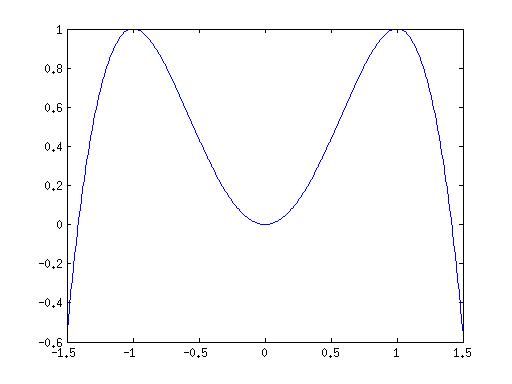
\includegraphics[scale=.35]{fig/es3-1a.jpg}\end{center}
\end{figure}
\item[b)]Il seguente codice è scritto nel file \verb1es3_2.m1 ed è lo script
che opera come richiesto:

\begin{codice}
\begin{verbatim}
A = zeros(8,8);
for i=7:-1:1
  A = A + diag(-i*(ones(i,1)),8-i);
end
\end{verbatim}
\end{codice}
Infatti, stampando la matrice $A$ si ha:
\begin{codice}
\begin{verbatim}
>> A

A =

     0    -7    -6    -5    -4    -3    -2    -1
     0     0    -7    -6    -5    -4    -3    -2
     0     0     0    -7    -6    -5    -4    -3
     0     0     0     0    -7    -6    -5    -4
     0     0     0     0     0    -7    -6    -5
     0     0     0     0     0     0    -7    -6
     0     0     0     0     0     0     0    -7
     0     0     0     0     0     0     0     0

\end{verbatim}
\end{codice}
Si effettua ora la costruzione della matrice $B$ come rischiesto, mediante
una semplice operazione algebrica sulle matrici:
\begin{codice}
\begin{verbatim}
>> B = A - A'

B =

     0    -7    -6    -5    -4    -3    -2    -1
     7     0    -7    -6    -5    -4    -3    -2
     6     7     0    -7    -6    -5    -4    -3
     5     6     7     0    -7    -6    -5    -4
     4     5     6     7     0    -7    -6    -5
     3     4     5     6     7     0    -7    -6
     2     3     4     5     6     7     0    -7
     1     2     3     4     5     6     7     0

>> 
\end{verbatim}
\end{codice}
Ora verifichiamo la simmetria, ricordiamo che una matrice $A$ è simmetrica
se e solo se $A \cdot A^{-1} = I$.
\begin{codice}
\begin{verbatim}
>> B * inv(B)

ans =

    1.0000    0.0000   -0.0000   -0.0000    0.0000   -0.0000    0.0000    0.0000
    0.0000    1.0000   -0.0000   -0.0000    0.0000    0.0000   -0.0000    0.0000
    0.0000         0    1.0000    0.0000   -0.0000    0.0000    0.0000    0.0000
   -0.0000    0.0000   -0.0000    1.0000   -0.0000    0.0000    0.0000   -0.0000
   -0.0000    0.0000   -0.0000   -0.0000    1.0000    0.0000   -0.0000   -0.0000
    0.0000    0.0000    0.0000   -0.0000   -0.0000    1.0000   -0.0000    0.0000
   -0.0000    0.0000   -0.0000   -0.0000         0    0.0000    1.0000   -0.0000
    0.0000   -0.0000    0.0000    0.0000    0.0000         0   -0.0000    1.0000

\end{verbatim}
\end{codice}
La matrice risulta simmetrica.
\end{itemize}
\end{svol}

\item Dopo aver visualizzato in Matlab il valore \verb1realmin1 $\simeq 10^{-m}$,
predisporre e visualizzare in \verb1format long e1 un vettore di $21$ elementi
logaritmicamente equispaziati fra $10^-m$ e $10^{-m-20}$. Commentare i
ruslitati ottenuti.  

\begin{svol}
\begin{codice}
\begin{verbatim}
>> realmin

ans =

  2.2251e-308

>> format long e
>> m = 308;
>> rm = logspace(-m,-m-20,21)

rm =

  Columns 1 through 3

    9.999999999999999e-309    1.000000000000002e-309    9.999999999999969e-311

  Columns 4 through 6

    9.999999999999475e-312    9.999999999984653e-313    1.000000000013287e-313

  Columns 7 through 9

    9.999999999638807e-315    9.999999984816838e-316    9.999999836597144e-317

  Columns 10 through 12

    1.000000230692537e-317    9.999987484955998e-319    9.999888671826830e-320

  Columns 13 through 15

    9.999888671826830e-321    9.980126045993180e-322    9.881312916824931e-323

  Columns 16 through 18

    9.881312916824931e-324                         0                         0

  Columns 19 through 21

                         0                         0                         0

>> 
\end{verbatim}
\end{codice}
Gli elementi del vettore \verb1er1 risultano equispaziati fino al sedicesimo 
elemento, dopodichè si ha il fenomeno di underflow.
\end{svol}

\item
Al variare del parametro $p=10^{\alpha}$, con $\alpha = 1:10$, calcolare mediante
le note formule risolutive, le radici dell'equazione di quarto grado:
\[
x^4 -bx^2 +1 = 0,
\]
con $b = \frac{1+p^2}{p}$. In seguito, dopo aver tradotto tali formule in
istruzioni di assegnazione Matlab, predisporre una tabella con gli errori 
relativi commessi da Matlab nel calcolo numerico delle radici dell'equazione 
assegnata. Motivare i risultati ottenuti.

\begin{svol}Iniziamo a calcolare le radici con le formule note:
\begin{codice}
\begin{verbatim}
>> p = logspace(1,10,10);
>> b = (1+p.^2)./p;
>> 
>> % Per risolvere x^4 -bx^2 + 1 = 0 poniamo t = x^2 e
>> % risolvo l'equazione t^2 - bt + 1 = 0
>> 
>> % Calcolo del delta
>> delta = sqrt(b.^2-4)./2;
>> 
>> % Calcolo dei due possibili valori di t
>> t1 = (b + delta)./2;
>> t2 = (b - delta)./2;
>> 
>> % Calcolo dei valori delle x
>> x1 = sqrt(t1);
>> x2 = -sqrt(t1);
>> x3 = sqrt(t2);
>> x4 = -sqrt(t2);
>>
>> % Inseriamo ora i risultati ottenuti in una tabella X
>> X = [x2' x1' x4' x3']

X =

   1.0e+04 *

  -0.000274317334487   0.000274317334487  -0.000160468065359   0.000160468065359
  -0.000866039837421   0.000866039837421  -0.000500074994376   0.000500074994376
  -0.002738613243961   0.002738613243961  -0.001581141201791   0.001581141201791
  -0.008660254052278   0.008660254052278  -0.005000000075000   0.005000000075000
  -0.027386127875715   0.027386127875715  -0.015811388303214   0.015811388303214
  -0.086602540378458   0.086602540378458  -0.050000000000075   0.050000000000075
  -0.273861278752584   0.273861278752584  -0.158113883008421   0.158113883008421
  -0.866025403784439   0.866025403784439  -0.500000000000000   0.500000000000000
  -2.738612787525831   2.738612787525831  -1.581138830084190   1.581138830084190
  -8.660254037844387   8.660254037844387  -5.000000000000000   5.000000000000000

\end{verbatim}
\end{codice}
Abbiamo così ottenuto una matrice contenente, per ogni riga, le quattro
radici del polinomio al variare del parametro $b$.

Calcoliamo ora le radici con il metodo di Matlab \verb1roots1 e calcoliamo 
l'errore assoluto tra le due soluzioni.
\begin{codice}
\begin{verbatim}
>> for i = 1 : 10
Roots(i,:) = roots([1 0 -b(i) 0 1]);
end
>> Roots

Roots =

   1.0e+05 *

  -0.000031622776602   0.000031622776602  -0.000003162277660   0.000003162277660
  -0.000100000000000   0.000100000000000  -0.000001000000000   0.000001000000000
  -0.000316227766017   0.000316227766017  -0.000000316227766   0.000000316227766
  -0.001000000000000   0.001000000000000  -0.000000100000000   0.000000100000000
  -0.003162277660168   0.003162277660168  -0.000000031622777   0.000000031622777
  -0.010000000000000   0.010000000000000  -0.000000010000000   0.000000010000000
  -0.031622776601684   0.031622776601684  -0.000000003162278   0.000000003162278
  -0.100000000000000   0.100000000000000  -0.000000001000000   0.000000001000000
  -0.316227766016838   0.316227766016838  -0.000000000316228   0.000000000316228
  -1.000000000000000   1.000000000000000   0.000000000100000  -0.000000000100000

>> Ea = abs(X-Roots)

Ea =

   1.0e+04 *

   0.000041910431530   0.000041910431530   0.000128845288757   0.000128845288757
   0.000133960162579   0.000133960162579   0.000490074994376   0.000490074994376
   0.000423664416207   0.000423664416207   0.001577978924130   0.001577978924130
   0.001339745947722   0.001339745947722   0.004999000075000   0.004999000075000
   0.004236648725969   0.004236648725969   0.015811072075448   0.015811072075448
   0.013397459621542   0.013397459621542   0.049999900000075   0.049999900000075
   0.042366487264254   0.042366487264254   0.158113851385645   0.158113851385645
   0.133974596215562   0.133974596215562   0.499999990000000   0.499999990000000
   0.423664872642549   0.423664872642550   1.581138826921912   1.581138826921912
   1.339745962155612   1.339745962155615   5.000000001000000   5.000000001000000

>> 
\end{verbatim}
\end{codice}
Errore relativo:
\begin{codice}
\begin{verbatim}
>> Er = abs((Roots-X)./X)

Er =

   0.152780835408468   0.152780835408469   0.802934144367142   0.802934144367141
   0.154681293851390   0.154681293851391   0.980002999325169   0.980002999325169
   0.154700345929209   0.154700345929209   0.998000002999993   0.998000002999993
   0.154700536454750   0.154700536454750   0.999800000003000   0.999800000003000
   0.154700538360007   0.154700538360007   0.999980000000003   0.999980000000003
   0.154700538379059   0.154700538379060   0.999998000000000   0.999998000000000
   0.154700538379250   0.154700538379250   0.999999800000000   0.999999800000000
   0.154700538379252   0.154700538379252   0.999999980000000   0.999999980000000
   0.154700538379252   0.154700538379252   0.999999998000000   0.999999998000000
   0.154700538379251   0.154700538379252   1.000000000200000   1.000000000200000

>> 
\end{verbatim}
\end{codice}
\end{svol}

\item In relazione al calcolo numerico della derivata di $f(x) = e^x$, in
$x = 1$, si considerino le seguenti approssimazioni:
\[
\frac{f(x+h)-f(x)}{h}, \ \frac{f(x+h)-f(x-h)}{2h}.
\]
Si indichi l'errore analitico per entrambe le discretizzazioni cosiderate
e si predispongano con Matlab, al variare del parametro $h = 10^{-\alpha}$,
$\alpha = 1, \ldots, 20$:
\begin{itemize}
\item[a)]una tabella in \verb1format short e1 contenente i valori di $h$ e i
corrispondenti errori analitici;
\item[b)]un grafico di tali errori in scala logaritmica.
\end{itemize}
Analizzare i risultati ottenuti.

\begin{svol}
\begin{itemize}
\item[a)]
Poniamo \verb1e1 come il valore $e^x$, con $x = 1$ e calcoliamo i valori delle
approssimazioni \verb1p1 utilizzando i parametri indicati.
\begin{codice}
\begin{verbatim}
>> e = exp(1);
>> for i=1:20
h(i) = 10^(-i);
end
>> 
>> p1 = (exp(1+h)-e)./h;
>> p2 = (exp(1+h)-exp(1-h))./(2*h);
>> 
>> e1 = e -p1;
>> e2 = e -p2;
>> 
>> O = [h; e1; e2];
>> fprintf('%e \t %e \t %e \n',O)
1.000000e-01 	 -1.405601e-01 	 -4.532735e-03 
1.000000e-02 	 -1.363683e-02 	 -4.530492e-05 
1.000000e-03 	 -1.359594e-03 	 -4.530467e-07 
1.000000e-04 	 -1.359186e-04 	 -4.530565e-09 
1.000000e-05 	 -1.359145e-05 	 -5.858736e-11 
1.000000e-06 	 -1.358527e-06 	 1.634577e-10 
1.000000e-07 	 -1.355058e-07 	 -5.858691e-11 
1.000000e-08 	 5.101167e-08 	 6.602751e-09 
1.000000e-09 	 2.286474e-07 	 6.602751e-09 
1.000000e-10 	 2.893183e-06 	 6.727366e-07 
1.000000e-11 	 1.177497e-05 	 -1.042949e-05 
1.000000e-12 	 1.177497e-05 	 -2.102696e-04 
1.000000e-13 	 4.896756e-03 	 4.558642e-04 
1.000000e-14 	 5.374657e-02 	 9.337648e-03 
1.000000e-15 	 5.374657e-02 	 -1.682980e-01 
1.000000e-16 	 2.718282e+00 	 4.978358e-01 
1.000000e-17 	 2.718282e+00 	 2.718282e+00 
1.000000e-18 	 2.718282e+00 	 2.718282e+00 
1.000000e-19 	 2.718282e+00 	 2.718282e+00 
1.000000e-20 	 2.718282e+00 	 2.718282e+00 
>> 
\end{verbatim}
\end{codice}

\end{itemize}
\end{svol}

\item
Usando il comando Matlab \verb1Hilb(n)1 costruire la matrice di Hilbert di 
ordine $10$. Costruire poi il vettore $b$ in modo che il sistema lineare 
$Hx = b$ abbia solunzione il vettore $x$ con tutte le componenti uguali a $1$.

Risolvere il sistema lineare $Hx = b$ usando i comandi Matlab. Costruire poi il
vettore $c= b + z$ dove $z^t = [0.001 0 \cdots 0]$ e risolvere il nuovo sistema
$Hy = c$.

Calcolare $e_r = \frac{\|x-y\|_2}{\|x\|_2} $.

\begin{svol}
Calcloiamo $H$ utilizzando il comando specificato, e mediante operazioni
elementari ricaviamo il vettore $b$ e quindi $x$.
\begin{codice}
\begin{verbatim}
>> H = hilb(10);
>> b = H*ones(10,1);
>> 
>> x = H\b

x =

   0.999999998715226
   1.000000110249369
   0.999997664058654
   1.000021147216568
   0.999899477767458
   1.000275541218743
   0.999549027556600
   1.000434891240842
   0.999772107416504
   1.000050035409456

>> 
\end{verbatim}
\end{codice}
Come si può notare il vettore $x$ è perturbato da errori algoritmici.

\begin{codice}
\begin{verbatim}
>> z = [0.001; zeros(9,1)];
>> c = b+z

c =

   2.929968253968254
   2.019877344877345
   1.603210678210678
   1.346800421800422
   1.168228993228993
   1.034895659895660
   0.930728993228993
   0.846695379783615
   0.777250935339171
   0.718771403175428

>> y = H\c

y =

   1.0e+03 *

   0.001099997010956
  -0.003949743297673
   0.080194557919823
  -0.599550712574902
   2.523285644515019
  -6.304657469284754
   9.609548217661349
  -8.749585606735506
   4.376268391416600
  -0.922663274650903

>> er = norm(x-y)/norm(x)

er =

     4.851631507736105e+0
\end{verbatim}
\end{codice}
\end{svol}

\end{enumerate}

\section{Esercitazione IV.}

\begin{enumerate}
\item
\begin{itemize}
\item[a)]Rappresentare graficamente su un intervallo $[a,b]$ la funzione
\[f(x) = 2 \sin(8x)-\ln(x^2+1)\]
usando una griglia di punti equispaziati dell'intervallo $[a,b]$.
\item[b)]Rappresentare la funzione $f(x)$ definita da:
\[f(x) = \left\{\begin{array}{lr}x^2&x\leq 3\\9&x > 3\end{array}\right.\]
sull'intervallo $[2,4]$.
\end{itemize}

\begin{svol}
\begin{itemize}
\item[a)]Svolgiamo l'esercizio utilizzando due griglie di punti ed usiamo
il comando \verb1plot1 per visualizzare i due grafici in una sola figura.
Cogliamo l'occasione per vedere la differenza di rappresentazione
di una funzione in base alla scelta del numero di punti.
\begin{codice}
\begin{verbatim}
>> % Definiamo il nostro intervallo [a,b] come per
>> % per il punto b), ovvero a = 2 e b = 4.
>> a = 2;
>> b = 4;
>> x = linspace(a,b,1000); 
>> 
>> % Calcoliamo ora la f(x) del punto a)
>> Fxa = 2*sin(8*x)-log(x.^2 +1);
>> 
>> % Proviamo ora a utilizzare una griglia con meno punti, per poi
>> % confrontarne i grafici.
>> x1 = linspace(a,b,20);
>> ya = 2*sin(8*x1)-log(x1.^2 +1);
>> 
>> % Stampa dei due grafici.
>> plot(x,Fxa,x1,ya,'r')
\end{verbatim}
\end{codice}
\begin{figure}[!ht]\begin{center}
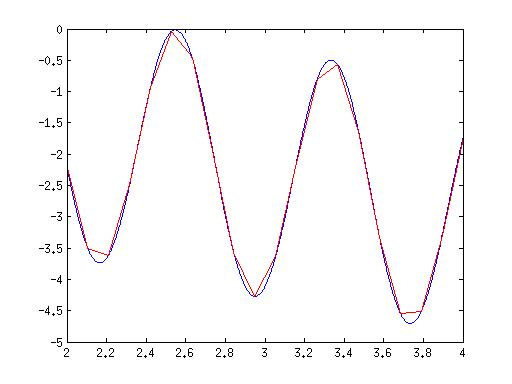
\includegraphics[scale=.50]{fig/es4-1a.jpg}\end{center}
\caption{esercizio $1$.a}
\end{figure}

\item[b)]Analogamente al punto a) vediamo due griglie.
\begin{codice}
\begin{verbatim}
>> % Calcoliamo ora l'intervallo per la funzione f(x) per il punto
>> % b) suddividendola in due intervalli x = x1b U x2b
>> x1b = linspace(2,3,500);
>> x2b = linspace(3,4,500);
>> 
>> % Calcoliamo ora i valori della funzione definita a tratti, escludendo il
>> % primo punto del primo vettore.
>> fxb1 = x1b.^2;
>> fxb2 = 9*ones(1,500);
>> 
>> % Ripetiamo i calcoli utilizzando meno punti.
>> x1bb = linspace(2,3,10);
>> x2bb = linspace(3,4,10);
>> 
>> fxbb1 = x1bb.^2;
>> fxbb2 = 9*ones(1,10);
>> 
>> % Stampiamo i grafici facendo attenzione ad escludere il primo punto
>> % della seconda parte del vettore.
>> plot(x1b,fxb1,x2b(2:500),fx2b(2:500), x1bb,fx1bb,'r',x2bb(2:10),fxbb2(2:10),'r')
??? Undefined function or method 'fx2b' for input arguments of type 'double'.
 
>> plot(x1b,fxb1,x2b(2:500),fxb2(2:500), x1bb,fx1bb,'r',x2bb(2:10),fxbb2(2:10),'r')
??? Undefined function or variable 'fx1bb'.
 
>> plot(x1b,fxb1,x2b(2:500),fxb2(2:500), x1bb,fxbb1,'r',x2bb(2:10),fxbb2(2:10),'r')
>> 
\end{verbatim}
\end{codice}
\begin{figure}[!ht]\begin{center}
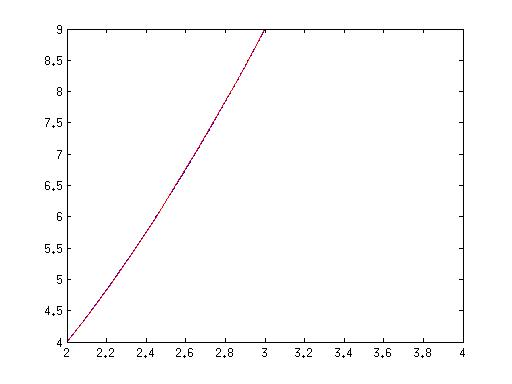
\includegraphics[scale=.50]{fig/es4-1b.jpg}\end{center}
\caption{esercizio $1$.b}
\end{figure}

\end{itemize}
\end{svol}

\item 
\begin{itemize}
\item[a)]
Dopo aver visualizzato in Matlab il valore \verb1realmin1 $\simeq 10^{-m}$,
predisporre e visualizzare in formato \verb1format long e1 un vettore di
$21$ elementi logaritmicamente equispaziati fra $10^{-m}$ e $10^{-m-20}$.
\item[b)]Visualizzare i valori \verb1realmax1, \verb1realmax1$\cdot 10$,
\verb1realmax1$\cdot (1+eps)$.
\item[c)]Visualizzare i valori $1+10^{-17}$ e $1 + 10^{17}$.
\end{itemize}

\begin{svol}
\begin{enumerate}
\item[a)]
\begin{codice}
\begin{verbatim}
>> format long e
>> realmin

ans =

    2.225073858507201e-308

>> logspace(-m,-m-20,21)'

ans =

    9.999999999999999e-309
    1.000000000000002e-309
    9.999999999999969e-311
    9.999999999999475e-312
    9.999999999984653e-313
    1.000000000013287e-313
    9.999999999638807e-315
    9.999999984816838e-316
    9.999999836597144e-317
    1.000000230692537e-317
    9.999987484955998e-319
    9.999888671826830e-320
    9.999888671826830e-321
    9.980126045993180e-322
    9.881312916824931e-323
    9.881312916824931e-324
                         0
                         0
                         0
                         0
                         0

\end{verbatim}
\end{codice}{\samepage
Con il comando \verb1logspace1 troviamo alcuni valori più piccoli di
\verb1realim1, che ricordiamo, è il più piccolo numero \emph{normalizzato} in
doppia precisione rappresentabile. Come si può vedere infatti, i numeri
trovati non sono normalizzati (non iniziano con un $1$ prima della virgola 
oppure hanno più zeri subito dopo) e di conseguenza è possibile utilizzare
più \verb1bits1 per l'esponente (o caratteristica) e meno per la mantissa.
Ad un certo punto la caratteristica esce comunque dal range ($p<-m$) e si
ha quindi il fenomeno dell'underflow.}
\item[b)]Valutiamo i seguenti risultati:
\begin{codice}
\begin{verbatim}
>> realmax

ans =

    1.797693134862316e+308

>> realmax*10

ans =

   Inf

>> realmax*(1+eps)

ans =

   Inf
\end{verbatim}
\end{codice}
Abbiamo qui il fenomeno di overflow.

\item[c)]
\begin{codice}
\begin{verbatim}
>> 1+10^17

ans =

     1.000000000000000e+17

>> 1+10^-17

ans =

     1

>> 
\end{verbatim}
\end{codice}
In questi due casi abbiamo il fenomeno di arrotondamento, e poiché
gli addendi di $1$ sono minori di $\frac{\beta}{2}$ i risultati
vengono troncati.
\end{enumerate}
\end{svol}

\item
Scrivere un file script in Matlab in grado di calcolare la ``precisione di
macchina'' in base $2$, ricordando che tale valore è caratterizzato come il 
più piccolo numero macchina positivo tale che $fl(1+eps) >1$.

\begin{svol}Lo script Matlab, salvato in un file di nome \verb1epsilon.m1
è il seguente:
\begin{codice}
\begin{verbatim}
epsi =1;
while (1+epsi)>1
    epsi = (1/2)*epsi;
end
epsi=epsi*2
\end{verbatim}
\end{codice}
Richiamando lo script nell'ambiente di lavoro si ha il seguente risultato:
\begin{codice}
\begin{verbatim}
>> eps

ans =

   2.2204e-16

>> epsilon

epsi =

   2.2204e-16

>> 
\end{verbatim}
\end{codice}
\end{svol}

\item
Vedere esercizio $3$ della terza esercitazione.

\item
Osservare l'andamento del resto nello sviluppo di Taylor seguente:
\[
\sin(x+1) = \sin(1) + \cos(1)\cdot x + R(x).
\]
Fare un grafico in scala logaritmica dell'andamento del resto in funzione
di $x$.

\begin{svol}
Per vedere l'andamento del resto, otteniamo mediante operazioni algebriche
i valori di $R(x) = s\in(x+1) - (\sin(1) +\cos(1)\cdot x$ su un'intervallo di 
punti logaritmicamente equispaziati.
\begin{codice}
\begin{verbatim}
>> x = logspace(-13,0,1000);
>> 
>> % Calcolo di R(x)
>> R = sin(x+1) - (sin(1) + cos(1).*x);
>> 
>> plot(x,R)
>> 
\end{verbatim}
\end{codice}


\begin{figure}[!ht]\begin{center}
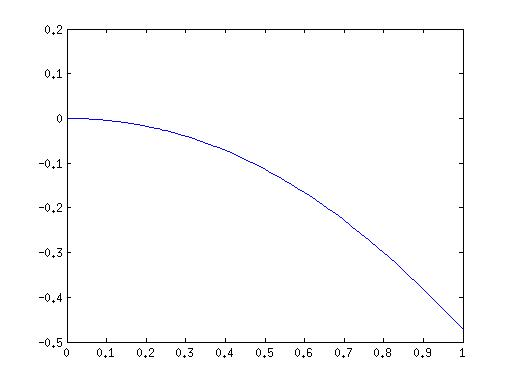
\includegraphics[scale=.50]{fig/es4-5.jpg}\end{center}
\caption{esercizio $5$}
\end{figure}
\end{svol}

\item Osservare la convergenza nel calcolo dei limiti delle seguenti
funzioni:
\begin{itemize}
\item $x \cdot (\sqrt{(x^2+1)}-x)$;
\item $x \cdot \sqrt{(x^2+1)}-x^2$;
\item $x / (\sqrt{(x^2+1)}+x)$.
\end{itemize}

\begin{svol}
Come nell'esercizio della sezione \ref{esercizio4-6} dedicata ai test
campione, si può notare che il limite a $+\infty$ tende ad $\frac{1}{2}$.
\begin{codice}
\begin{verbatim}
>> x = logspace(-13,0,15);
>> 
>> f1 = x.*(sqrt(x.^2 + 1)-x);
>> f2 = x.*sqrt(x.^2+1)-x.^2;
>> f3 = x./(sqrt(x.^2 + 1) +x);
>> 
>> % Creo un vettore di output y (matrice)
>> y = [x; f1; f2; f3];
>> 
>> % funzione di stampa
>> format long e
>> fprintf('%.3e %18.16f %18.16f %18.16f \n',y)
1.000e-13 0.0000000000001000 0.0000000000001000 0.0000000000001000 
8.483e-13 0.0000000000008483 0.0000000000008483 0.0000000000008483 
7.197e-12 0.0000000000071969 0.0000000000071969 0.0000000000071969 
6.105e-11 0.0000000000610540 0.0000000000610540 0.0000000000610540 
5.179e-10 0.0000000005179475 0.0000000005179475 0.0000000005179475 
4.394e-09 0.0000000043939705 0.0000000043939705 0.0000000043939705 
3.728e-08 0.0000000372759358 0.0000000372759358 0.0000000372759358 
3.162e-07 0.0000003162276660 0.0000003162276660 0.0000003162276660 
2.683e-06 0.0000026826885984 0.0000026826885984 0.0000026826885984 
2.276e-05 0.0000227579413192 0.0000227579413192 0.0000227579413192 
1.931e-04 0.0001930325005496 0.0001930325005496 0.0001930325005496 
1.638e-03 0.0016352132081426 0.0016352132081426 0.0016352132081426 
1.389e-02 0.0137032264540035 0.0137032264540035 0.0137032264540035 
1.179e-01 0.1047980301759449 0.1047980301759449 0.1047980301759449 
1.000e+00 0.4142135623730951 0.4142135623730951 0.4142135623730951 
\end{verbatim}
\end{codice}
Intuitivamente dai valori della tabella stampata sulla command window il limite
tende a $0$, vediamo un grafico tabulando con $1000$ punti ancora più
vicini a a $0$.
\begin{codice}
\begin{verbatim}
>> x = logspace(-15,0,1000);
>> f1 = x.*(sqrt(x.^2 + 1)-x);
>> f2 = x.*sqrt(x.^2+1)-x.^2;
>> f3 = x./(sqrt(x.^2 + 1) +x);
>> plot(x,f1)
>> xlabel('x')
>> 
>> plot(x,f1)
>> xlabel('asse delle ascisse')
>> 
\end{verbatim}
\end{codice}

\begin{figure}[!ht]\begin{center}
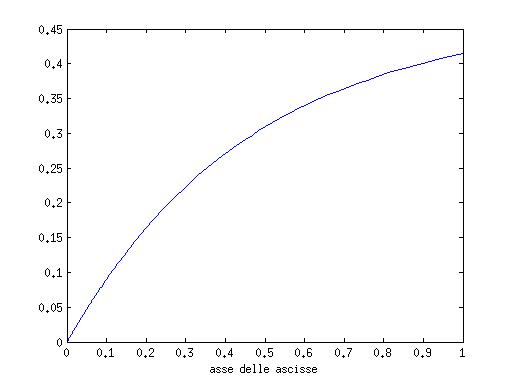
\includegraphics[scale=.50]{fig/es4-6.jpg}\end{center}
\caption{esercizio $6$, si può notare che $\displaystyle \lim_{x \to o}f(x)=0$.}
\end{figure}

\end{svol}
\end{enumerate}

\section{Esercitazione V.}

\begin{enumerate}

\item Studiare il condizionamento della funzione $f(x) = \cos(x)$. Fornire
esempi numerici che motivino i risultati ottenuti.

\begin{svol}
Studiare il condizionamento significa valutare se un problema è ben
condizionato, ovvero se a piccole perturbazioni sui dati corrispondono
errori dello stesso ordine.

Sia $x$ un dato, e $\tilde{x}$ lo stesso dato affetto da errore, $\Delta x =
\tilde{x}-x$.
\[
\textrm{Imponiamo } \Delta x = 10^{-13}, \textrm{ ovvero } 10^{-8} = \tilde{x} 
- x \Rightarrow \tilde{x} = 10^{-8} +x.
\]
Posto $y = \cos(x)$ e $\tilde{y} = \cos(\tilde{x})$, il problema è
trovare $\Delta y = \tilde{y} - y$. Dalla definizione e passando allo sviluppo
di Taylor si ha:
\[
\tilde{y} = f(x + \Delta x) = f(x) + f'(x)\Delta x + \cdots
\]
\[\tilde{y} - f(x) = f'(x)\Delta x + \cdots \]
da cui segue che $\Delta y = \tilde{y} - y \simeq f'(x)\Delta x$.

Tornando ai dati del problema si ha:
\[\Delta y = -\sin(x)\cdot 10^{-13}.\]
Poiché l'immagine della funzione $\sin$ è l'intervallo $[-1,1]$ possiamo
concludere che:
\[
\Delta y \subseteq [-1,1]\cdot 10^{-13} = [-10^{-8},10^{-8}].
\]
Da questo deduciamo che l'errore assoluto non cambia ordine di grandezza,
tuttavia noi vogliamo valutare l'errore relativo sui dati, ovvero trovare
$\frac{\Delta y}{y}$.

Valutiamo ora l'indice di condizionamento:
\[\frac{x}{\cos(x)}\cdot (-1)\sin(x) = -x \cdot \tan(x).\]
Da questo possiamo notare che, ad esempio in un intorno di $\frac{\pi}{2}$ 
l'indice di condizionamento ``esplode'' diventando $\simeq \infty$.

Vediamo quindi con Matlab il nostro caso:
\[
\frac{\Delta y}{y} = \frac{x}{f(x)}Df(x)\frac{\Delta x}{x} = 
\frac{\pi}{\cos(\pi)}(-1)\sin(\pi)\frac{10^{-8}}{\pi}.
\]
\begin{codice}
\begin{verbatim}
>> x = pi/2;
>> y = cos(x)

y =

     6.123233995736766e-17

>> 
>> deltax = 10^(-8);
>> 
>> xt = x - deltax;
>> yt = cos(xt)

yt =

     1.000000000045763e-08

\end{verbatim}
\end{codice}
Già il confronto tra questi due risultati ci dice che il divario tra le due 
soluzioni è eccessivamente elevato.
\begin{codice}
\begin{verbatim}
>> deltay = y-yt

deltay =

    -9.999999939225290e-09

>> deltay_ = -sin(x)*deltax

deltay_ =

    -1.000000000000000e-08

\end{verbatim}
\end{codice}
Qui sopra possiamo notare che, sia utilizzando la soluzione algebrica 
$\Delta y = y -\tilde{y}$ che quella analitica, l'ordine di grandezza
dell'errore relativo non cambia da quello di partenza sui dati.
\begin{codice}
\begin{verbatim}
>> % Calcolo dell'errore relativo sui dati.
>> erx = deltax/x;
>>
>> % Calcolo dell'indice di condizionamento cond.
>> cond = (x/cos(x))*(-sin(x));
>> 
>> % Errore relativo sui risultati.
>> ery = cond*erx

ery =

    -1.633123935319537e+08

>> 
\end{verbatim}
\end{codice}
L'ordine dell'errore relativo sui risultati è, in valore assoluto, di $10^8$,
molto più elevato di quello sui dati di partenza. Il problema è malcondizionato.
\end{svol}

\item Si approssimi il valore di $e^{-9}$, utilizzando lo sviluppo in serie
di $e^{x}$:
\[
e^x = 1 + x + \frac{x^2}{2!} + \frac{x^3}{3!} + \cdots 
\]
Quanti termini sono necessari per stabilizzare il risultato a $6$ cifre?

Ripetere il calcolo ricordando che è possibile scrivere $e^{-x} = \frac{1}{e^x}$.
Costruire, per un confronto, una tabella e un grafico degli errori relativi dei 
valori ottenuti sommando $n$ termini usando i due diversi algoritmi.

\begin{svol} Con due cicli \verb1while1 calcoliamo l'approssimazione di
$e^{-9}$ con una tolleranza \verb1t1 dell'ordine di $10^{-6}$, stampiamo quindi
il valore di \verb1i1 che rappresenta il numero di termini utilizzati.
\begin{codice}
\begin{verbatim}
>> format long
>> d = exp(-9);
>> x = -9;
>> a1 = 1 + x;
>> 
>> err = d-a1;
>> t = 10^-6;
>> i = 2;
>> 
>> while(abs(err)>t)
a1 = a1 + (x^i)/factorial(i);
err = d - a1;
i = i + 1;
end
>> i

i =

    34

>> a1

a1 =

     1.226613221354248e-04

>> d

d =

     1.234098040866796e-04

>> x = 9;
>> s = 1 + x;
>> a = 1/s;
>> err = d - a;
>> i = 2;
>> t = 10^-6;
>> while(abs(err)>t)
s = s + (x^i)/factorial(i);
a = 1/s;
err = d - a;
i = i + 1;
end;
>> i

i =

    18

>> a

a =

     1.240698022398142e-04

\end{verbatim}
\end{codice}
Il primo metodo impiega ben $34$ termini, mentre il secondo quasi la metà,
questo ci dice che la convergenza del primo è più lenta.

Calcoliamo ora due vettori contenenti le prime $34$ approssimazioni secondo
i due metodi e confrontiamole.
\begin{codice}
\begin{verbatim}
>> x = 9;
>> 
>> a1 = 1;
>> i = 2;
>> a1(2) = 1 - x;
>>
>> for i=3:35
a1(i) = a1(i-1) + ((-x)^(i-1))/factorial(i-1);
end
>> a1(35)

ans =

     1.236033868055714e-04

>> s = 1 + x;
>> a2 = 1;
>> a2(2) = 1/s;
>>
>> s(2) = 1 + x;
>> 
>> for i=3:35
s(i) = s(i-1) + (x^(i-1))/factorial(i-1);
a2(i) = 1/s(i);
end
>> a2(34)

ans =

     1.234098041059322e-04

>> d = exp(-9)

d =

     1.234098040866796e-04

>> ea1 = d - a1;
>> ea2 = d - a2;
>> er1 = ea1/d;
>> er2 = ea2/d;
>> 
>> [er1', er2']

ans =

   1.0e+06 *

  -0.008102083927575  -0.008102083927575
   0.064825671420603  -0.000809308392758
  -0.263349227646200  -0.000159457107477
   0.721175469554209  -0.000046110953067
  -1.494005099146711  -0.000017193845473
   2.493319924514945  -0.000007643750523
  -3.487667610977539  -0.000003836038004
   4.202173506084228  -0.000002087401582
  -4.448897750610261  -0.000001194654415
   4.202173506084228  -0.000000702393539
  -3.583790624940812  -0.000000416454028
   2.786543664079675  -0.000000245317013
  -1.991207052685690  -0.000000141847842
   1.316466520459563  -0.000000079739600
  -0.809895062276671  -0.000000043260166
   0.465921887365069  -0.000000022532170
  -0.251725146808410  -0.000000011230636
   0.128205635989315  -0.000000005348020
  -0.061759755409548  -0.000000002432304
   0.028223851042545  -0.000000001057070
  -0.012268771860897  -0.000000000439445
   0.005085209383436  -0.000000000174982
  -0.002014146580155  -0.000000000066832
   0.000763862275163  -0.000000000024520
  -0.000277891045581  -0.000000000008653
   0.000097140149887  -0.000000000002941
  -0.000032678340852  -0.000000000000964
   0.000010594489394  -0.000000000000305
  -0.000003314634614  -0.000000000000093
   0.000001001990078  -0.000000000000028
  -0.000000292997329  -0.000000000000008
   0.000000082966757  -0.000000000000002
  -0.000000022773142  -0.000000000000001
   0.000000006065012  -0.000000000000000
  -0.000000001568617  -0.000000000000000

>> n = linspace(1,35,35);
>> plot(n,er1,n,er2,'r');
>> 
\end{verbatim}
\end{codice}
Il primo metodo ha una convergenza molto più lenta, inoltre, come si può
vedere dal grafico, l'errore oscilla costantemente mentre nel secondo
questo fenomeno non si verifica.
\begin{figure}[!ht]\begin{center}
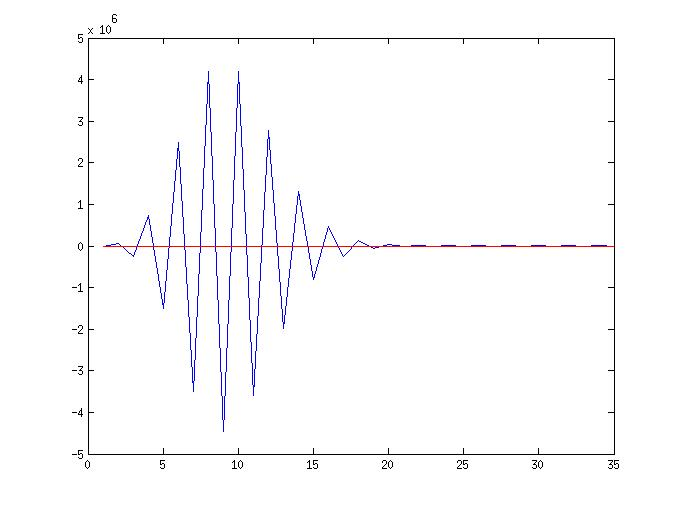
\includegraphics[scale=.50]{fig/es5-2.jpg}\end{center}
\caption{esercizio $2$.}
\end{figure}
\end{svol}

\item Siano $A = \text{hilb}(1000)$ e $B = \text{rand}(1000)$.
\begin{itemize}
\item[a)]Costruire il vettore $b$ in modo che il sistema $Ax = b$ sia risolto
da $x = \text{ones}(1000,1)$, e il vettore $c$ in modo che il sistema $By = c$
sia risolto da $y = \text{ones}(1000,1)$;
\item[b)]Calcolare i vettori $x$ e $y$ come soluzione dei sistemi lineari 
$Ax = b$ e $By = c$ utilizzando il comando \verb1\ (mldivide)1 di Matlab;
\item[c)]Calcolare gli errori relativi rapportandoli al numero di 
condizionamento delle corrispondenti matrici. Cosa si osserva?
\item[d)]Rappresentare in un grafico in scala semilogaritmica il condizionamento
della matrice di Hilbert di dimensioni variabili da $2 \times 2$ a $50 \times 
50$.
\end{itemize}

\begin{svol}Costruiamo le matrici come indicato.

\begin{codice}
\begin{verbatim}
>> H = hilb(1000);
>> B = rand(1000);
\end{verbatim}
\end{codice}

\begin{itemize}
\item[a)]
Calcoliamo i vettori $c$ e $b$ mediante prodotto riga per colonna delle
matrici e dei vettori costruiti, sfruttando la simmetria della relazione 
``$=$''.
\begin{codice}
\begin{verbatim}
>> x = ones(1000,1);
>> y = ones(1000,1);
>> 
>> b = A*x;
>> c = B*y;
\end{verbatim}
\end{codice}

\item[b)]Calcoliamo i vettori soluzione dei sistemi lineari di cui sopra
$x_1$ e $y_1$, per distinguerli da quelli iniziali.
\begin{codice}
\begin{verbatim}
>> x1 = A\b;
Warning: Matrix is close to singular or badly scaled.
         Results may be inaccurate. RCOND = 1.878903e-22. 
>> y1 = B\c;
>> 
\end{verbatim}
\end{codice}
Matlab già ora ci avverte che i risultati su $x_1$ potrebbero essere
affetti da errore.
\item[c)] Utilizziamo il comando \verb1cond()1 per calcolare l'indice di
condizionamento delle due matrici, calcoliamo quindi gli errori relativi
sulle soluzioni.
\begin{codice}
\begin{verbatim}
>> ca = cond(A)

ca =

   3.6665e+21

>> cb = cond(B)

cb =

   2.8027e+05

>> eax = x - x1;
>> eay = y - y1;
>> erx = erx./x;
>> ery = ery./y;
>> 
>> max(abs(erx))

ans =

   1.2879e+04

>> max(abs(ery))

ans =

   6.2221e-12

\end{verbatim}
\end{codice}
L'indice di condizionamento della matrice $A$ è molto elevato, infatti 
il massimo dell'errore relativo in modulo è molto più elevato di quello
calcolato per il vettore $y$ relativo alla matrice $B$, che ha infatti un 
indice di condizionamento molto minore.
\item[d)] Calcoliamo l'indice di condizionamento delle matrici di Hilbert
come richiesto e salviamole nel vettore \verb1CondH1. Utilizziamo quindi il
comando \verb1semilogy()1 che disegna il grafico in scala semilogaritmica
lungo l'asse delle $y$, utilizzando una scala lineare per l'asse delle $x$.
\begin{codice}
\begin{verbatim}
>> for i=2:50
CondH(i) = cond(hilb(i));
end
>> semilogy(CondH)
\end{verbatim}
\end{codice}
\begin{figure}[!ht]\begin{center}
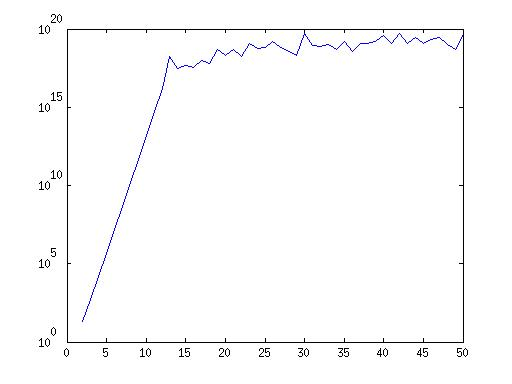
\includegraphics[scale=.50]{fig/es5-3.jpg}\end{center}
\caption{esercizio $3$.}
\end{figure}
\end{itemize}
\end{svol}

\item
Data la matrice $A$, e i vettori $b$, $x^*$ tali che:
\[
A = \left[ 
\begin{array}{cccc}
-4 & -1 & 1 & 1 \\
0 & -4 & -1 & 1 \\
-1 & -1 & 4 & 1 \\
1 & -1 & 0 & 4
\end{array}
\right], \quad 
b = \left[ 
\begin{array}{c}
-3  \\
-4 \\
3 \\
4
\end{array}
\right], \quad 
x^* = \left[ 
\begin{array}{c}
1  \\
1 \\
1 \\
1
\end{array}
\right];
\] 
preso un vettore $x^{(0)} \in \rr^{4}$ arbitrario, calcolare e tabulare al 
variare di $k = 0, \ldots, 10$, le seguenti quantità:
\[
\|x^*-x^{(k)}\|_1,\quad \|x^*-x^{(k)}\|_2,\quad \|x^*-x^{(k)}\|_\infty,
\]
dove
\[
x^{(k+1)} = (I-D^{-1}A)x^{(k)} + D^{-1}b, \quad k = 0, \ldots, 10.
\]
$I$ è la matrice identità e $D^{-1}$ è l'inversa della matrice diagonale $D$ 
estratta dalla matrice $A$. Mettere in un grafico la tabella costruita nella
prima parte dell'esercizio.

\begin{svol}
Iniziamo ad impostare i dati.
\begin{codice}
\begin{verbatim}
>> A = [-4 -1 1 1; 0 -4 -1 1; -1 -1 4 1; 1 -1 0 4]

A =

    -4    -1     1     1
     0    -4    -1     1
    -1    -1     4     1
     1    -1     0     4

>> b = [-3; -4; 3; 4];
>> x_ = ones(4,1);
>> 
>> D = diag(diag(A))

D =

    -4     0     0     0
     0    -4     0     0
     0     0     4     0
     0     0     0     4

>> I = eye(4);
>> Dinv = inv(D);
>>
>> x = rand(4,1);
\end{verbatim}
\end{codice}
Ora costruiamo la matrice contente i vettori $x^{(k+1)}$ e quella con
$x^*-x^{(k)}$.
\begin{codice}
\begin{verbatim}
>> for i=2:10
x(:,i) = (I-Dinv*A)*x(:,i-1) + Dinv*b;
end
>>
>> % le colonne di ex sono i vettori x-x^k
>> for i=1:10
ex(:,i) = x_ - x(:,i); 
end
\end{verbatim}
\end{codice}
Infine calcoliamo le tre norme per ogni $k$ richiesto e stampiamo la tabella
relativa.
\begin{codice}
\begin{verbatim}
>> for i=1:10
n1(i) = norm(ex(:,i));
n2(i) = norm(ex(:,i),2);
n1(i) = norm(ex(:,i),1);
ninf(i) = norm(ex(:,i),inf);
end
>> O = [linspace(1,10,10);n1;n2;ninf];
>> fprintf('\n k\t Norma 1 \t Norma 2 \t Norma Inf\n\n'),...
fprintf('%i \t %1.6f \t %1.6f \t %1.6f\n', O)

 k	 Norma 1 	 Norma 2 	 Norma Inf

1 	 2.444721 	 1.294401 	 0.902460
2 	 0.473086 	 0.262154 	 0.204245
3 	 0.185871 	 0.113172 	 0.101262
4 	 0.071560 	 0.043558 	 0.029724
5 	 0.022182 	 0.015684 	 0.014769
6 	 0.013994 	 0.008012 	 0.005531
7 	 0.005840 	 0.003309 	 0.002223
8 	 0.001676 	 0.001079 	 0.000921
9 	 0.001095 	 0.000568 	 0.000346
10 	 0.000443 	 0.000272 	 0.000191
>> 
\end{verbatim}
\end{codice}
\end{svol}

\end{enumerate}


\section{Esercitazione VI.}

\begin{enumerate}

\item
Determinare i coefficienti $a_i$ dei polinomi di grado $10$, $15$ e $20$ 
interpolanti la funzione $f(x) = e^x +1$ nei nodi equispaziati dell'intervallo
$[-1,1]$ (suggerimento: usare la matrice di Vandermonde e poi risolvere il
sistema lineare). Successivamente considerare i nuovi dati perturbati
$\tilde{f}(x_i) = f(x_i) + \varepsilon_i$ con $\varepsilon_i = (-1)^i10^{-5}$ e
calcolare i coefficienti $\tilde{a}_i$ del polinomio perturbato $\tilde{p}(x)$
interpolante i dati $(x_i, \tilde{f}(x_i))$. Confrontare i grafici dei due
polinomi.

Calcolare:
\[
\max |a_i - \tilde{a}_i| \quad \text{e} \quad \max |p(t)-\tilde{p}(t)|
\]
dove $t$ è un vettore formato da $101$ punti equispaziati in $[-1,1]$.

Ripetere l'esercizio usando i nodi di Chebishev:
\[x_i = \cos\left(\frac{(2i+1)\pi}{2n+2}\right), \quad i = 1,\ldots, n.\]
Commentare i risultati ottenuti.

\begin{svol}
Iniziamo con il calcolo dei tre grafici con punti equispaziati.
\begin{codice}
\begin{verbatim}
>> % Per avere polinomi di grado N occorrono N+1 punti.
>> x10 = linspace(-1,1,11);
>> x15 = linspace(-1,1,16);
>> x20 = linspace(-1,1,21);
>> 
>> % Costruzione delle matrici di Vandermonde.
>> V10 = vander(x10);
>> V15 = vander(x15);
>> V20 = vander(x20);
>> 
>> % Costruizione delle immagini della funzione.
>> b10 = exp(x10)+1;
>> b15 = exp(x15)+1;
>> b20 = exp(x20)+1;
>> 
>> % Calcolo dei coefficienti a dei polinomi.
>> a10 = V10\b10';
>> a15 = V15\b15';
>> a20 = V20\b20';
>> 
>> % Introduciamo i vettori delle perturbazioni
>> for i = 1 : 11
eps10(i) = ((-1)^i)*10^(-5);
end
>> for i = 1 : 16
eps15(i) = ((-1)^i)*10^(-5);
end
>> for i = 1 : 21
eps20(i) = ((-1)^i)*10^(-5);
end
>> 
>> % Calcolo delle immagini della funzione perturbate
>> b10_p = b10 + eps10;
>> b15_p = b15 + eps15;
>> b20_p = b20 + eps20;
>> 
>> % Calcolo dei coefficienti perturbati
>> a10_p = V10\b10_p';
>> a15_p = V15\b15_p';
>> a20_p = V20\b20_p';
>> 
>> % t è il vettore  di punti in cui valutare i polinomi.
>> t = linspace(-1,1,101);
>>
>> % Valutazione dei polinomi al variare di t.
>> y10 = polyval(a10, t);
>> y15 = polyval(a15, t);
>> y20 = polyval(a20, t);
>>
>> % Valutazione dei polinomi perturbati al variare di t.
>> y10_p = polyval(a10_p, t);
>> y15_p = polyval(a15_p, t);
>> y20_p = polyval(a20_p, t);
>>
>> % Stampa.
>> plot(t, y10, t, y10_p,'r');
>> plot(t, y15, t, y15_p,'r');
>> plot(t, y20, t, y20_p,'r');
>> 
\end{verbatim}
\end{codice}

Gli errori massimi sui coefficienti e sulle valutazioni dei polinomi
 sono i seguenti:
\begin{codice}
\begin{verbatim}
>> format long
>> % Calcolo degli errori.
>> E_coeff = [max(abs(a10-a10_p)) max(abs(a15-a15_p)) max(abs(a20-a20_p))]

E_coeff =

   1.0e+03 *

   0.000057870370372   0.011238023832376   2.568468176961571

>> E_y = [max(abs(y10-y10_p)) max(abs(y15-y15_p)) max(abs(y20-y20_p))]

E_y =

   0.000291264924889   0.005083726754011   0.106893964401543

>> 
\end{verbatim}
\end{codice}

Vediamo ora con i nodi di Chebishev come si comportano i nostri polinomi.
\begin{codice}
\begin{verbatim}
>> for i = 1 : 11
cheb10(i) = cos(((2*(i-1)+1)*pi)/(2*10+2));
end
>> for i = 1 : 16
cheb15(i) = cos(((2*(i-1)+1)*pi)/(2*15+2));
end
>> for i = 1 : 21
cheb20(i) = cos(((2*(i-1)+1)*pi)/(2*20+2));
end
>> 
>> for i = 1 : 21
cCheb20(i) = cos(((2*(i)+1)*pi)/(2*21+2));
end
>> 
>> 
>> V10_c = vander(cheb10);
>> V15_c = vander(cheb15);
>> V20_c = vander(cheb20);
>> 
>> b10_c = exp(cheb10)+1;
>> b15_c = exp(cheb15)+1;
>> b20_c = exp(cheb20)+1;
>> 
>> a10_c = V10_c\b10_c';
>> a15_c = V15_c\b15_c';
>> a20_c = V20_c\b20_c';
>> 
>> b10_cp = b10_c + eps10;
>> b15_cp = b15_c + eps15;
>> b20_cp = b20_c + eps20;
>> 
>> a10_cp = V10_c\b10_cp';
>> a15_cp = V15_c\b15_cp';
>> a20_cp = V20_c\b20_cp';
>> 
>> t = linspace(-1,1,101);
>> y10_c = polyval(a10_c,t);
>> y10_cp = polyval(a10_cp,t);
>> plot(t, y10_c, t, y10_cp,'r');
>> 
>> y15_c = polyval(a15_c,t);
>> y15_cp = polyval(a15_cp,t);
>> plot(t, y15_c, t, y15_cp,'r');
>> 
>> y20_c = polyval(a20_c,t);
>> y20_cp = polyval(a20_cp,t);
>> plot(t, y20_c, t, y20_cp,'r');
>> 
\end{verbatim}
\end{codice}


\begin{figure}[!ht]\begin{center}
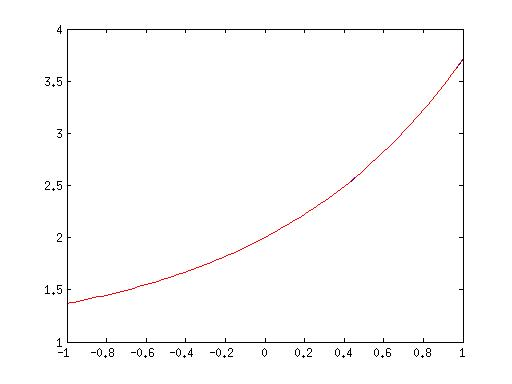
\includegraphics[scale=.35]{fig/es6-1a.jpg}
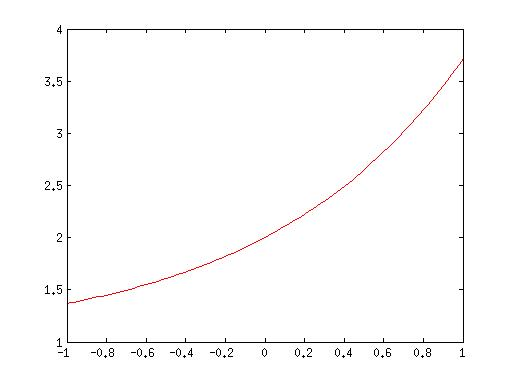
\includegraphics[scale=.35]{fig/es6-1d.jpg}
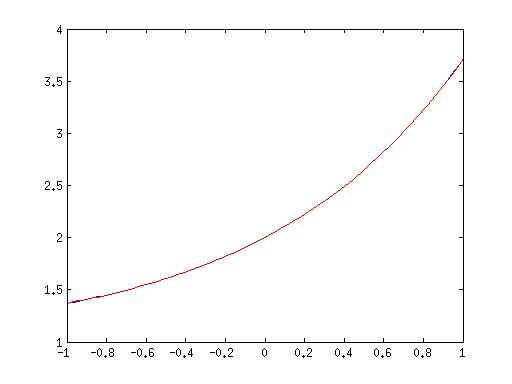
\includegraphics[scale=.35]{fig/es6-1b.jpg}
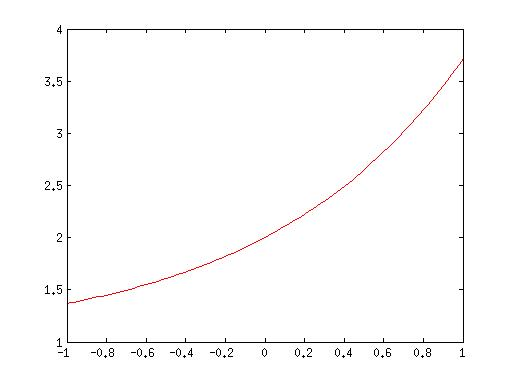
\includegraphics[scale=.35]{fig/es6-1e.jpg}
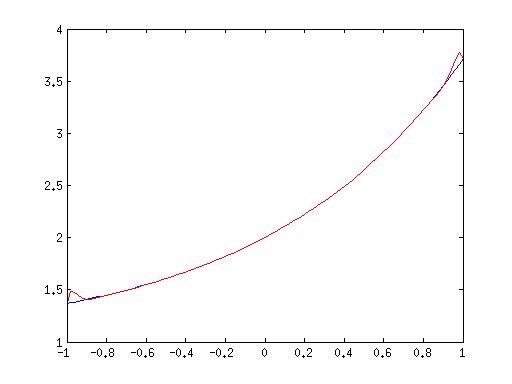
\includegraphics[scale=.35]{fig/es6-1c.jpg}
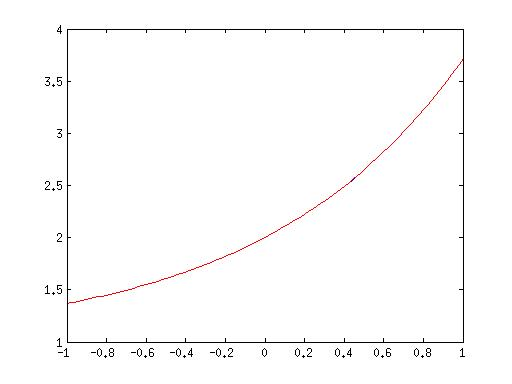
\includegraphics[scale=.35]{fig/es6-1f.jpg}
\end{center}
\caption{Sulla sinistra vediamo la curva calcolata con i nodi equispaziati,
sulla destra con i nodi di Chebishev.}
\end{figure}
Analizzando gli errori n modulo si ha:
\begin{codice}
\begin{verbatim}
> E_y = [max(abs(y10_c-y10_cp)) max(abs(y15_c-y15_cp)) max(abs(y20_c-y20_cp))]

E_y =

   1.0e-04 *

   0.248943037695071   0.272777793646206   0.290082490588262

>> E_coeff = [max(abs(a10_c-a10_cp)) max(abs(a15_c-a15_cp)) max(abs(a20_c-a20_cp))]

E_coeff =

   0.015792758827331   1.120696937190668  79.113672059826612

>> 
\end{verbatim}
\end{codice}

Dai grafici si può notare che all'aumentare del numero dei punti nel polinomio
interpolatore calcolato con nodi equispaziati l'errore aumenta (sopratutto
agli estremi), mentre con i nodi di Chebyshev questo fenomeno non si verifica.

Inoltre i grafici di sinistra hanno linee più distanti rispetto a quelli
di destra, purtroppo lo zoom non è sufficiente, però ad occhio si può notare,
oltre alla differenza agli estremi, che le curve di sinistra sembrano più
``spesse''. Questo perchè sono più distanti e quindi meno precise, come
l'analisi sugli errori ha evidenziato.
\end{svol}

\item Approssimare la radice quadrata di $x = 0.6$ considerando l'interpolazione
nella forma di Lagrange con nodi i tre quadrati perfetti $x_0 = 0.49$, 
$x_1 = 0.64$ e $x_2 = 0.81$. Stimare il resto di interpolazione e calcolare lo 
scarto rispetto al valore ottenuto con il comando \verb1sqrt1 di Matlab. 

Ripetere le operazioni aggiungendo il nodo $x = 0.36$.

\begin{svol}
Per stimare l'errore occorre calcolare la derivata terza nel caso dei
$3$ punti assegnati e quindi applicare il teorema dell'errore, o resto.
\[
|e(x)| = \frac{|f^{(n+1)}(\xi_x)|}{(n+1)!}|\omega_n(x)|
\leq \frac{M}{(n+1)!}|\omega_n(x)| \leq \frac{M}{(n+1)!}(b-a)^{n+1}.
\]

\[
|e(x)| \leq \frac{1}{6}\cdot\frac{3}{8\cdot\xi_x^{\frac{5}{2}}}\cdot(0.81-0.49)^{3}
\]

Per calcolare $\xi_x$ usiamo un vettore equispaziato tra $0.49$ e $0.81$.
\begin{codice}
\begin{verbatim}
>> x = [0.49 0.64 0.81];
>> y = sqrt(x);
>> 
>> p = polyfit(x,y,2);
>> 
>> polyval(p,0.6);
>> root = polyval(p,0.6)

root =

    0.7744

>> r = sqrt(0.6)

r =

    0.7746

>> err = abs(r-root)

err =

   1.8490e-04

>> vett = linspace(0.49,0.81);
>> M = max(abs(3./(8*sqrt(vett.^5))))

M =

    2.2312

>> ex = (M/6)*(0.81-0.49)^3

ex =

    0.0122
\end{verbatim}
\end{codice}
Come si può notare \verb1ex1 è un'approssimazione corretta (anche se poco 
precisa) dell'errore \verb1err1.

Ora vediamo cosa accade aggiungendo il dato come richiesto, analogamente per
il calcolo dell'errore prendiamo un $\xi_x$ compreso tra $0.36$ e $0.81$.
\begin{codice}
\begin{verbatim}
>> 
>> 
>> x1 = [0.36 0.49 0.64 0.81];
>> y1 = sqrt(x1);
>> 
>> p1 = polyfit(x1,y1,3);
>> 
>> root1 = polyval(p1,0.6)

root1 =

    0.7747

>> err1 = abs(r-root1)

err1 =

   6.3964e-05

>>
>> vett1 = linspace(0.36,0.81);
>> M1 = max(abs(-15./(16*sqrt(vett1.^7))))

M1 =

   33.4898

>> ex1 = (M1/6)*(0.81-0.36)^3

ex1 =

    0.5086

>> 

\end{verbatim}
\end{codice}
Aumentando la distanza tra due punti la precisione dell'approssimazione
dell'errore peggiora, come ci aspettavamo.
\end{svol}

\item
Disegnare sull'intervallo $[-1,1]$ il grafico della funzione $|\omega_n(x)|
= \prod_{i=0}^n(x-x_i)$ per alcuni valori di $n$ considerando nodi equispaziati.
Ripetere l'esercizio considerando i nodi di Chebyshev. Confrontare sullo
stesso sistema di riferimento i due grafici.

\begin{svol}
Iniziamo a definire queste due funzioni per costruire i nodi di Chebishev
e per calcolare la funzione $\omega_n$ dato un vettore di nodi.
\begin{codice}
\begin{verbatim}
function [x] = chebyshev(a,b,n)
%chebyshev calcola n nodi di chebyshev

for i=1:n
    x(i) = ((b-a)/2)*cos((2*i-1)*pi/(2*n+2)) + (a+b)/2; 
end

end


function [y] = omega_x(x, vec)
% omega_x := prod(x-x_i)

 n = length(x);
 y = zeros(n,1);
 for i = 1 : n
 y(i) = prod(x(i)-vec);
 end
 
end

\end{verbatim}
\end{codice}
A questo punto creiamo un vettore di dati e due vettori di nodi e vediamo
i risultati.
\begin{codice}
\begin{verbatim}
>> dati = linspace(-1,1,200);
>> 
>> nodi_e = linspace(-1,1,21);
>> nodi_c = chebyshev(-1,1,21);
>> 
>> y_e = omega_x(dati, nodi_e);
>> y_c = omega_x(dati, nodi_c);
>> 
>> plot(dati, y_e);
>> plot(dati, y_c);
>> 
>> plot(dati, y_e, dati, y_c, 'r');
>> 
\end{verbatim}
\end{codice}
\begin{figure}[!ht]\begin{center}
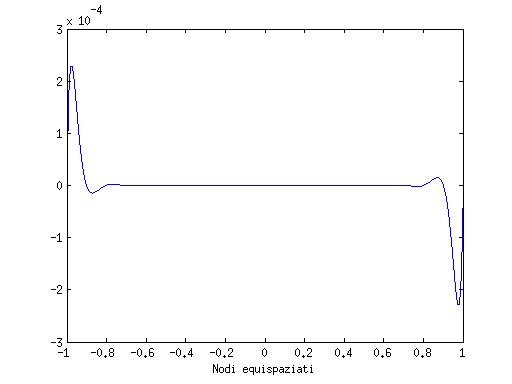
\includegraphics[scale=.35]{fig/es6-3a.jpg}
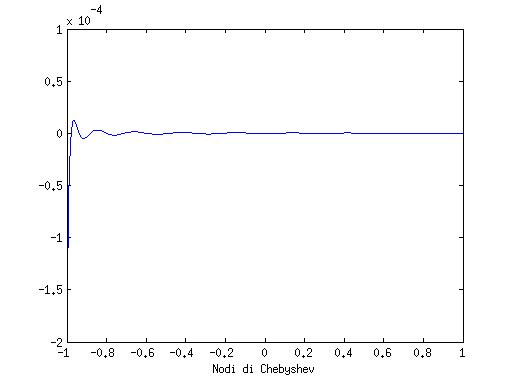
\includegraphics[scale=.35]{fig/es6-3b.jpg}
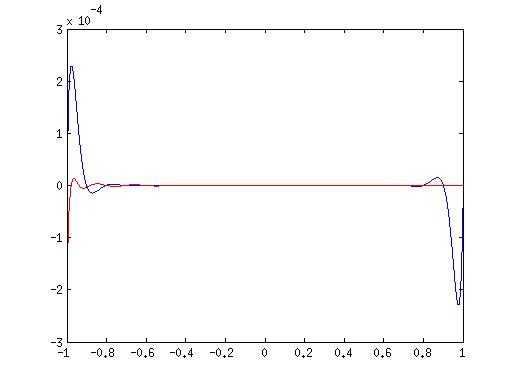
\includegraphics[scale=.35]{fig/es6-3c.jpg}
\end{center}
\end{figure}
\end{svol}

\end{enumerate}

\section{Esercitazione VII.}

\begin{enumerate}

\item 
Date le coppie di valori $(x_i,y_i)$, $i=0,\ldots,n$, ottenuti tabulando a 
passo costante le funzioni $y(x) = \sin(2 \pi x)$ e $y = \frac{1}{1 + 
25(2x -1)^2}$ sull'intervallo $[0,1]$, costruire le seguenti funzioni lineari:
\[
s(x) = y_i + m_i(x-x_i), \quad m_i = \frac{y_{i+1}-y_i}{x_{i+1}-x_i}, \quad
x \in [x_i,x_{i+1}], \ i = 0, \ldots, n-1
\]
e il polinomio interpolatore di Lagrange $p(x)$ di grado $n$.

Indicato con $x_i^* = \frac{x_i + x_{i+1}}{2}$ il punto medio di ciascun 
sottointervallo, tabulare l'errore assoluto:
\[
e_i^s = y(x_i^*) - s(x_i^*), \quad e_i^p = y(x_i^*) - p(x_i^*), \qquad
i = 0, \ldots, n-1.
\] 

Successivamente fare il grafico delle funzioni $s(x)$, $p(x)$, $y(x)$ 
sull'intervallo $[0,1]$.

\begin{svol}

\end{svol}


\end{enumerate}

%% -- Ambiente codice
\begin{comment}

\begin{codice}
\begin{verbatim}

\end{verbatim}
\end{codice}

\end{comment}
%% -- fine Ambiente codice

\chapter{Esercizi.}

\begin{ese}
\'E data la seguente tabella di valori:
\[
\begin{array}{cccccc}
x & -1 & 0 & \alpha & 2 & 3 \\
y & -1 & 0 & 1 & -1 & -1
\end{array}
\]
dove $\alpha$ è un parametro reale diverso da $-1$, $0$, $2$ e $3$.

Calcolare con un massimo errore assoluto: $e_a = 10^{-3}$, i valori di 
$\alpha$ che rendono minimo il \emph{grado} del polinomio che interpola 
i punti assegnati.

\begin{flushleft}\emph{Suggerimento:} Costruire la tabella delle differenze
divise contenente anche $\alpha$.
\end{flushleft}
\end{ese}

\part{Appendice.}
\label{Appendici}
\appendix
\label{Appendice}
%\addtocontents{toc}{\protect\contentsline{chapter} {Appendice}{}}
\hyphenation{
Barrow
Binet
Chebyshev
Cholesky
Cramer
Gauss
Faber
Frobenius
Hausdorff
Householder
Laplace
Lebesque
Newton
Rolle
Runghe
Sturm
tras-for-ma-zio-ne
Torricelli
}

%\addtocontents{toc}{\protect\contentsline{chapter} {Appendice}{}}
\chapter{Norme.}
\section{Norma di un vettore.}
La norma di un vettore è un'applicazione $\|\cdot\| \colon \rr^n \to \rr^+$
tale che:
\begin{itemize}
\item[$(1)$]$\|x\| \geq 0, \quad \forall x \in \rr^n$.
\item[$(2)$]$\|x\| = 0 \Leftrightarrow x = 0$.
\item[$(3)$]$\|ax\| = |a|\cdot\|x\|, \quad \forall x \in \rr^n$.
\item[$(4)$]$\forall x,y \in \rr^n \quad \|x+y\| \leq \|x\| + \|y\|$.
\end{itemize}

\begin{defi}Si definisce la
norma $p$ con $1 \leq p < +\infty$ tale che:
\[\|x\|_p = \left(\sum_{i=1}^n|x_i|^p \right)^{\frac{1}{p}}.\]
\[\|x\|_\infty = \max_{1 \leq i \leq m}|x_i|.\]
\end{defi}

\begin{exe}
Sia $x = (1, -2)$.
\[\|x\|_1 = 3, \quad \|x\|_2 = \sqrt{5}, \quad \|x\|_\infty = 2.\]
\end{exe}

\begin{defi}Due norme si dicono \emph{topologicamente equivalenti} se
esistono due costanti $\alpha, \beta \in \rr, 0 < \alpha \leq \beta$ tali che:
\[
\alpha \|x\|'' \leq \|x\|' \leq \beta\|x\|'.
\] 
\end{defi}

\begin{teo}
$\forall x \in \rr^n$ si ha:
\begin{enumerate}
\item $\|x\|_\infty \leq \|x\|_2 \leq \sqrt{n}\|x\|_\infty$.
\item $\|x\|_2 \leq \|x\|_1 \sqrt{n}\|x\|_2$.
\item $\|x\|_\infty \leq \|x\|_1 \leq n\|x\|_\infty$.
\end{enumerate}
\end{teo}

\section{Norma di una matrice.}
La norma di una matrice è un'applicazione analoga a quella sui vettori, 
valgono tutti i punti di cui sopra e in aggiunta:
\begin{itemize}
\item[$(5)$] $\|A\cdot B\| \leq \|A\|\cdot\|B\|$.
\end{itemize}

\begin{exe}Esempio di norma che non soddisfa la proprietà $(5)$:
\[
A = B = \left[\begin{array}{cc}1 & 1 \\ 0 & 1\end{array}\right], \quad
C = AB = \left[\begin{array}{cc}1 & 2 \\ 0 & 1\end{array}\right].
\]
\[
\max_{i,j}|c_{i,j}| = 2, \quad \max_{i,j}|a_{i,j}| = \max_{i,j}|b_{i,j}| = 1.
\]
\[2 \leq 1 \ \longrightarrow\ \textrm{Assurdo.} \]
\end{exe}

\begin{defi}
Si dice \emph{norma naturale} o \emph{norma indotta da un vettore} della
matrice $A$ il numero reale $\|A\|$ tale che:
\[
\|A\|= \sup_{x \neq 0}\frac{\|Ax\|}{\|x\|}.
\]
\end{defi}
\subsubsection{Proprietà:}
\begin{itemize}
\item[$(1)$]$\|I\| =1$.
\item[$(2)$]$\|Ax\| \leq \|A\|\|x\|$.
\item[$(3)$]$\rho(A)\leq \|A\|$.
\end{itemize}

$\rho(A)$ è il massimo autovalore di $A$ in modulo.

\begin{flushleft}
Nel condizionamento:
\[
1 = \|I\| = \|A\cdot A^{-1}\| \leq \|A\|\cdot\|A\| = 
\textrm{cond(}A\textrm{)}.
\]
\end{flushleft}

\begin{prop}
La norma naturale indotta da $\|\cdot\|_1$ è tale che:
\[
\left\|A\right\|_1 = \max_j \sum_{i = 1}^n|a_{i,j}|, \qquad A \in \rr^{n\times n}.
\]
\end{prop}
\begin{dimo}
\[ \left\|Ax\right\|_1  =  \left\| \sum_{j=1}^n a_{i,j}x_j\right\|_1 \]
\[ =  \sum_{i=1}^n\left|\sum_{j=1}^n a_{i,j}x_j\right| \leq  
\sum_{i=1}^n\sum_{j=1}^n |a_{i,j}||x_j| \]
\[ =  \sum_{j=1}^n|x_j|\sum_{i=1}^n |a_{i,j}|
\leq  \sum_{i=1}^n|x_j| \max_j\sum_{i=1}^n |a_{i,j}| \]
\[ =  \|x\|_1 (\max_j\sum_{i=1}^n |a_{i,j}|). \]

\[
\longrightarrow \ \frac{\|Ax\|_1}{\|x\|_1} \leq \sum_{i=1}^n |a_{i,j}|.
\]
\end{dimo}


\subsubsection{Norme indotte:}
\begin{enumerate}
\item $\|A\|_1 = \max_j \sum_{i=1}^n|a_{i,j}|$.
\item $\|A\|_2 = \sqrt{\rho(A^TA)}$. 
\item $\|A\|_\infty = \max_i \sum_{j=1}^n|a_{i,j}|$.
\end{enumerate}

\subsection{Norma di Frobenius.}
\begin{defi}
Sia $A \in \rr^{n \times n}$, la \emph{norma di Frobenius} è definita come 
segue:
\[
\|A\|_F = \left( \sum_{i=1}^n\sum_{j=1}^na_{i,j}^2\right)^{\frac{1}{2}}.
\]
\end{defi}
E' una norma compatibile con la norma due di vettore.
\[
\|A\|_2 \leq \|A\|_F\|x\|_2.
\]
La sintassi del comando Matlab, data una matrcie quadrata $X$, è la seguente:
\begin{codice}
\begin{verbatim}
>>> norm(X,'fro')
\end{verbatim}
\end{codice}

\subsubsection{Proprietà:}

\begin{enumerate}
\item $\frac{1}{\sqrt{n}}\|A\|_\infty \leq \|A\|_2 \leq \sqrt{n}\|A\|_\infty$.
\item $\frac{1}{\sqrt{n}}\|A\|_1 \leq \|A\|_2 \leq \sqrt{n}\|A\|_1$.
\item $\max_{i,j} |a_{i,j}| \leq \|A\|_2 \leq n \max_{i,j}|a_{i,j}|$.
\item $\|A\|_2 \leq \sqrt{\|A\|_1 \|A\|_\infty}$.
\end{enumerate}


\end{document}

